%%%%%%%%%%%%%%%%%%%%%%%%%%%%%%%%%%%%%%%%%%%%%%%%
\chapter{Object and event reconstruction}
\label{ch:EventReconstruction}
%%%%%%%%%%%%%%%%%%%%%%%%%%%%%%%%%%%%%%%%%%%%%%%%

In the pp collisions at the LHC a large number of particles are produced which must be efficiently reconstructed and identified. These particles travel through the CMS detector and they are classified as objects depending on their specific signature in each sub-detector. This chapter covers the reconstruction of physics objects that are needed for the identification of signal events in the lepton plus jet event topology described in Chapter~\ref{ch:dibosonIntro}.

The measurement of tracks in the tracker detector for charged particles and the reconstruction of the primary vertices represent key aspects of the reconstruction of the various objects and are detailed in Section~\ref{sec:tracksandvtx}. Details on the methods for reconstructing electrons, muons and jets present in the final states of these analyses are given, respectively, in Sections~\ref{sec:electrons}, \ref{sec:muons}, and \ref{sec:jets}. %In this analysis $\tau$ leptons are reconstructed as electrons (Section~\ref{sec:electrons}) or muons (Section~\ref{sec:muons}) and accounted to the respective channel if they decay leptonically, or as jets (Section~\ref{sec:jets}) if they decay hadronically. However, only the leptonic decay mode contributes to the analysis since at least one muon or electron has to be reconstructed in the event.
%However, the resulting gain in sensitivity is limited by the small branching ratios.
In addition to leptons and jets, the last type of particle present in the final state is the neutrino, whose presence can be inferred from an imbalance of the transverse momentum (Section~\ref{sec:met}).
The identified lepton and the missing transverse energy in the event are associated with the $\PW\to\ell\Pgn$ candidate which is reconstructed through the algorithms described in Section~\ref{sec:leptonicW}.

%%%%%%%%%%
%\section{Tracks and vertices}\label{sec:tracksandvtx}
 %%%%%%%%%%%%%%%%%%%%%%%%%%%%%%%%%%%%%%%%%%%%%%%%%%%%%%%%%%%%%%%
\section{Tracks and vertices}\label{sec:tracksandvtx}
%%%%%%%%%%%%%%%%%%%%%%%%%%%%%%%%%%%%%%%%%%%%%%%%%%%%%%%%%%%%%%%

The reconstruction of tracks of charged particles allows for their momentum measurement and aids in particle identification as described later. The reconstruction of the tracks' vertices is important to distinguish the primary interaction, i.e. the hard interaction, from additional interactions that might take place in the event and also for the identification of secondary vertices of jets that contain c or b quarks called c-/b-tagging (see Sec.~\ref{subsec:bjets}).

\subsection{Track reconstruction}\label{subsec:tracks}

The track reconstruction at CMS~\cite{Chatrchyan:2014fea} is based essentially on information coming from the silicon tracker system. A charged particle passing through a tracker layer can in general induce a signal in more than one pixel or more than one strip. The first step of the tracking procedure is the clusterization which assembles nearby tracker channels into one hit cluster. The particle position and its uncertainty is then inferred from the relative signal amplitudes in each channel.
%Despite the good performances and resolutions of the detectors, the track reconstruction is challenging due to the high density of tracks, to the presence of additional pileup vertices in each bunch crossing and to the amount of detector material leading to multiple scattering, energy loss and nuclear interactions.

Due to the magnetic field charged particles travel through the tracking detectors on a helix trajectory which is described by 5 parameters: the curvature $k$, the track azimuthal angle $\phi$ and polar angle $\theta$, the signed transverse impact parameter $d_0$ and the longitudinal impact parameter $z_0$. The transverse (longitudinal) impact parameter of a track is defined as the transverse (longitudinal) distance of closest approach of the track to the primary vertex.

The trajectories of charged particles are reconstructed through a iterative procedure which consists in multiple iterations of the {\itshape Combinatorial Track Finder algorithm} (CTF)~\cite{Adam:934067}, which uses the reconstructed hits in the silicon detectors to determine the track parameters. In the first iterations the algorithm searches for tracks of relative large \pt and produced near the interaction region. Then, hits associated to high quality tracks are iteratively removed from the input list to reduce the combinatorial complexity of the next iterations and to allow the more difficult reconstruction of low \pt or displaced tracks. Each iteration of the CTF algorithm is made of four steps: track seeding, track finding and track fitting.

In the first step, a first estimate of the helix parameters and of its covariance matrix is provided using only pairs or triplets of hits compatible with the hypothesis of a track coming from the p-p interaction region. Track candidates are best seeded from hits in the pixel detector because of the low occupancy, high efficiency and unambiguous 3-dimensional position information.

The track finding stage associates new hits in the next tracker layers to the trajectory obtained from seeds using a standard Kalman Filter (KF) pattern recognition approach~\cite{Billoir:1989mh,Fruhwirth:1987fm} which takes into account the effect of multiple scattering in the tracker layers. The current trajectory is extrapolated to the next tracker layer and compatible hits are assigned to the track on the basis of the $\chi^2$ between the predicted and measured positions. In case multiple compatible hits are found when extrapolating the helix to a single layer, the algorithm creates one trajectory candidate for each hit and they are propagated independently. Furthermore, in order to take into account possible inefficiencies one additional candidate is created without including any hit information. The tracks are assigned a quality based on the $\chi^2$, the number of missing hits and how compatible they are with originating from a primary interaction vertex. Only the best quality tracks are kept for further propagation and ambiguities are resolved between tracks during and after track finding. In case two tracks share more than 50\% of their hits, the lower quality track is discarded.  The fake rate, defined as the fraction of reconstructed tracks not associated with a charged particle, is substantially reduced through these quality requirements.

For each trajectory the finding stage results in an estimate of the track parameters. However, since the full information is only available at the last hit and constraints applied during trajectory building can bias the estimate of the track parameters, all valid tracks are refitted using the KF to determine the most accurate estimate of the helix parameters. The usual fit starting from the interaction point to the end of the tracker is complemented with a second fit run backward from the outermost tracker layer to the interaction point. This approach is found to improve the accuracy of the \pt and impact parameter measurement by 0.5\% and 1\% respectively.

%Figure~\ref{fig:track_eff} shows the tracking reconstruction efficiency as a function of $\eta$ for simulated muons, electrons, and pions.
%The tracking reconstruction efficiency has been measured to be $> 99\%$ for the isolated muons with $1 < \pt < 100\GeV$ in the $|\eta| < 2.5$ range, from 98\% to 89\% for 10\GeV pions and over 92\% for $>10\GeV$ electrons, as shown in Fig.~\ref{fig:track_eff}. 
The performance of the track reconstruction is shown in Fig.~\ref{fig:track_eff} for simulated muons, electrons and pions.
For isolated muons with $1 < \pt < 100\GeV$, the track reconstruction efficiency is $>$ 99\% over the full $\eta$-range of tracker acceptance, and does not depend on \pt (Fig.~\ref{fig:track_eff_a}). The fake rate is completely negligible. For pions and electrons the efficiency is in general lower along with a higher fake rate because of interactions with the material in the tracker. The material budget of the CMS tracker in units of radiation length is presented in Fig.~\ref{fig:budgetCMStracker}.

\begin{figure}[!htb]
\centering
\subfigure[]{\label{fig:track_eff_a}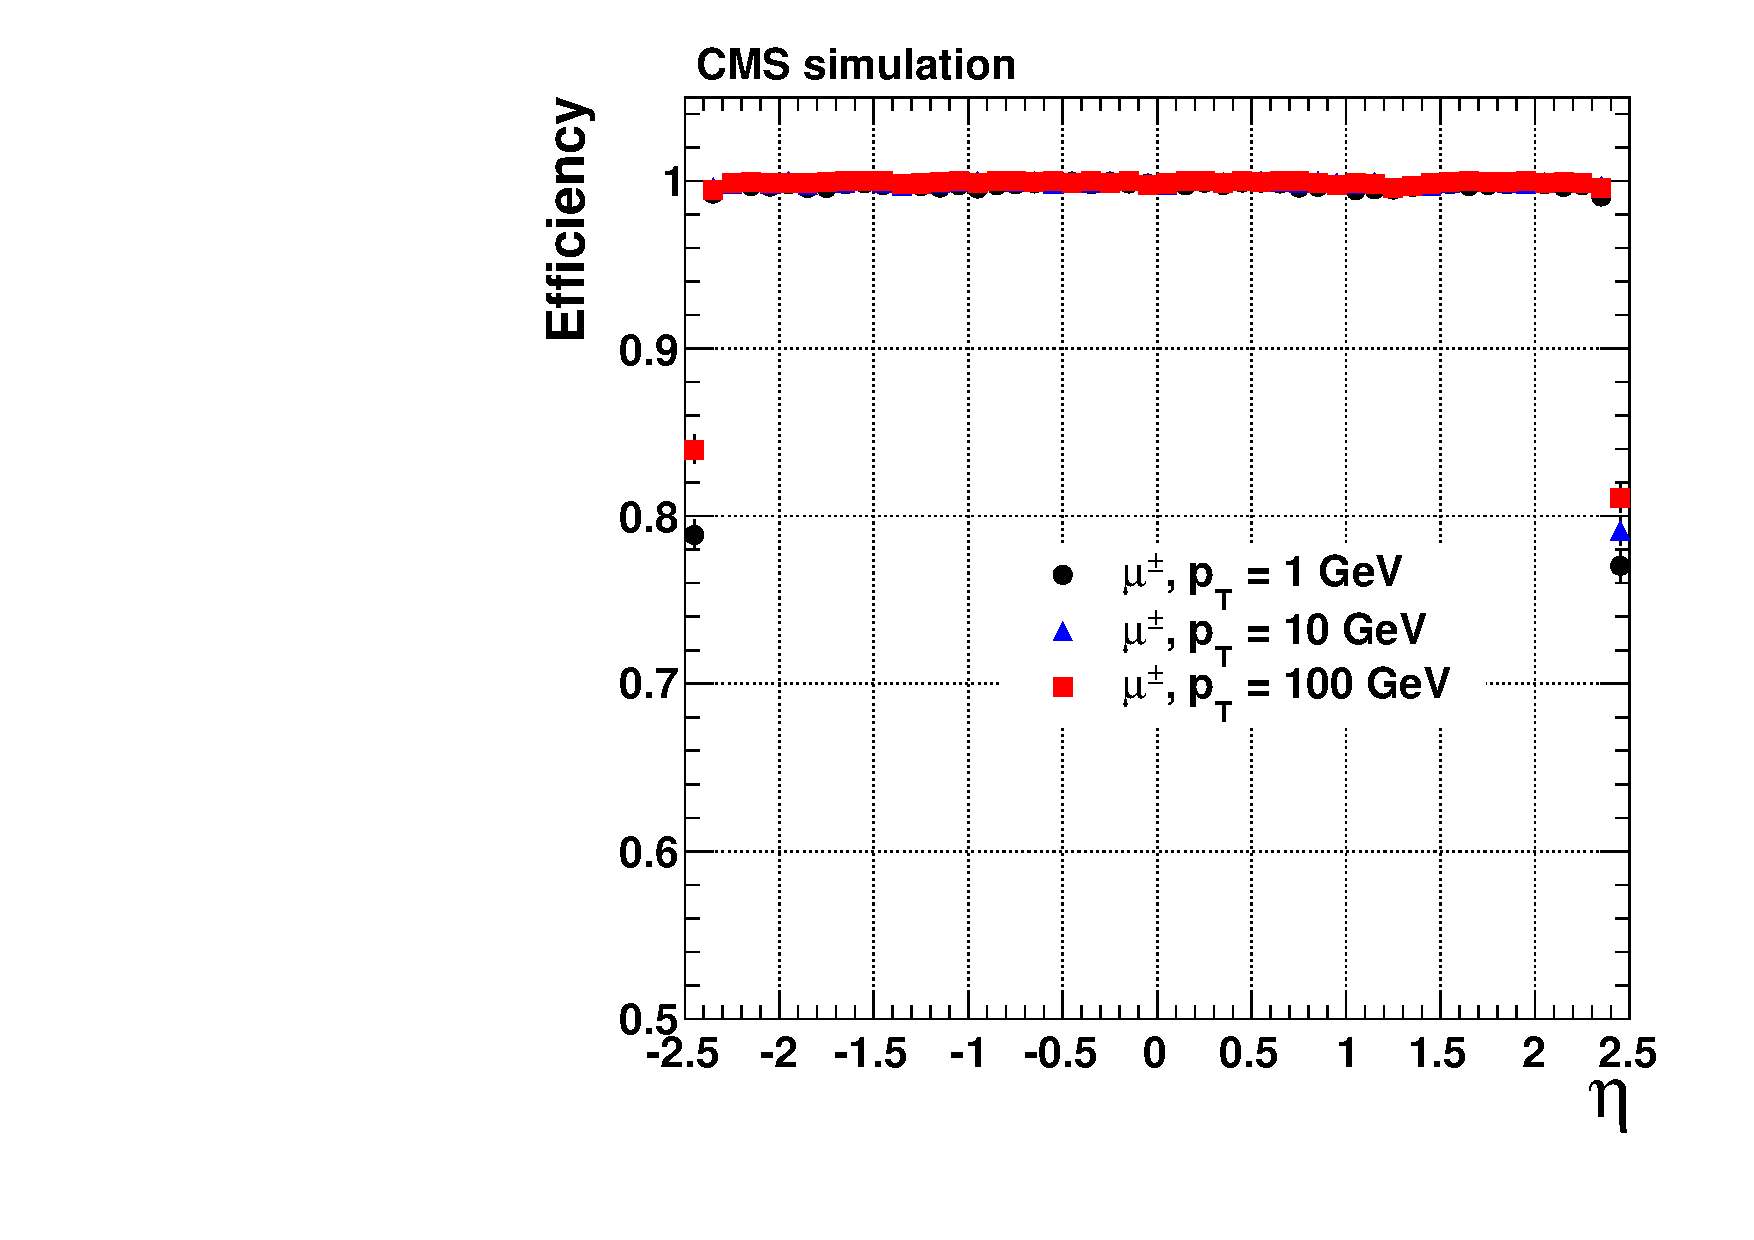
\includegraphics[width=0.30\textwidth]{\chsix/mu-efficiencyVsEta.pdf}}
\subfigure[]{\label{fig:track_eff_b}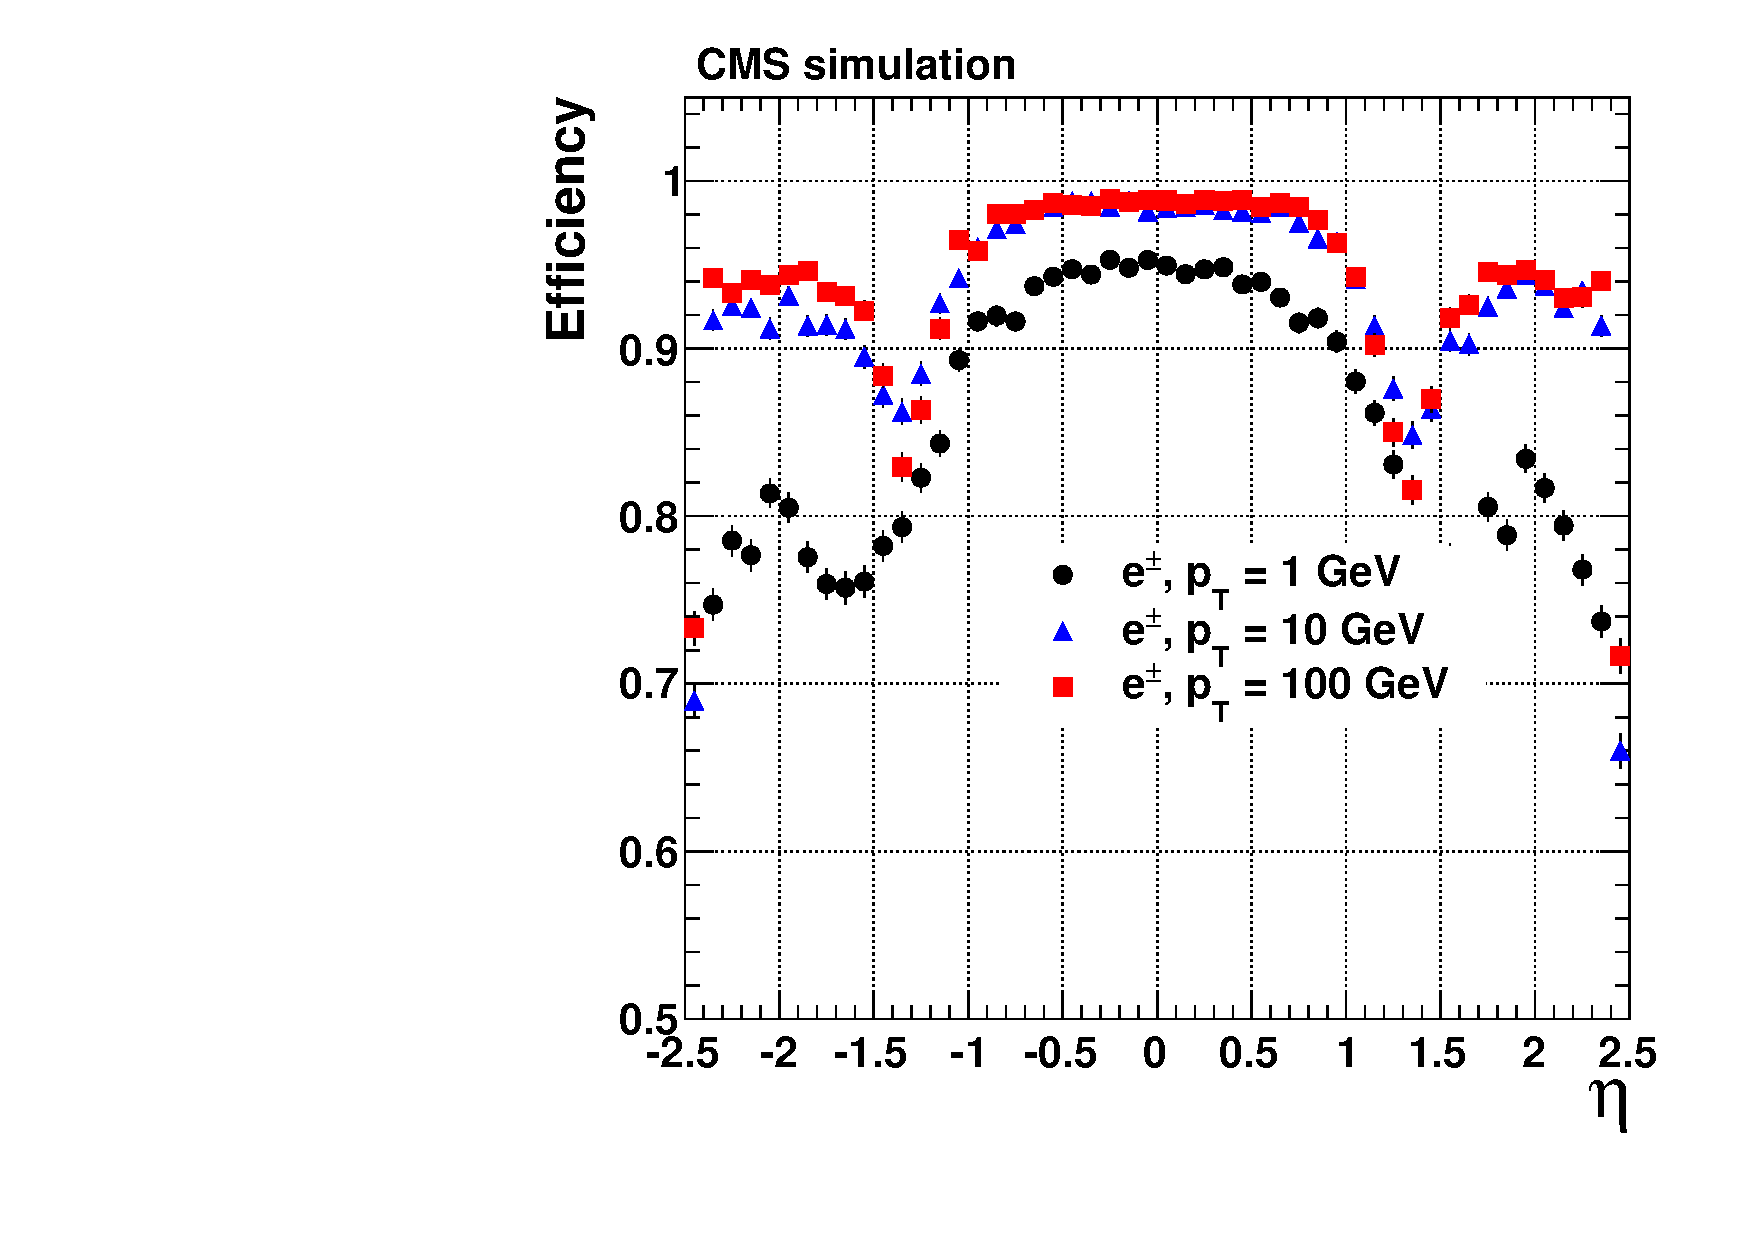
\includegraphics[width=0.30\textwidth]{\chsix/el-efficiencyVsEta.pdf}}
\subfigure[]{\label{fig:track_eff_c}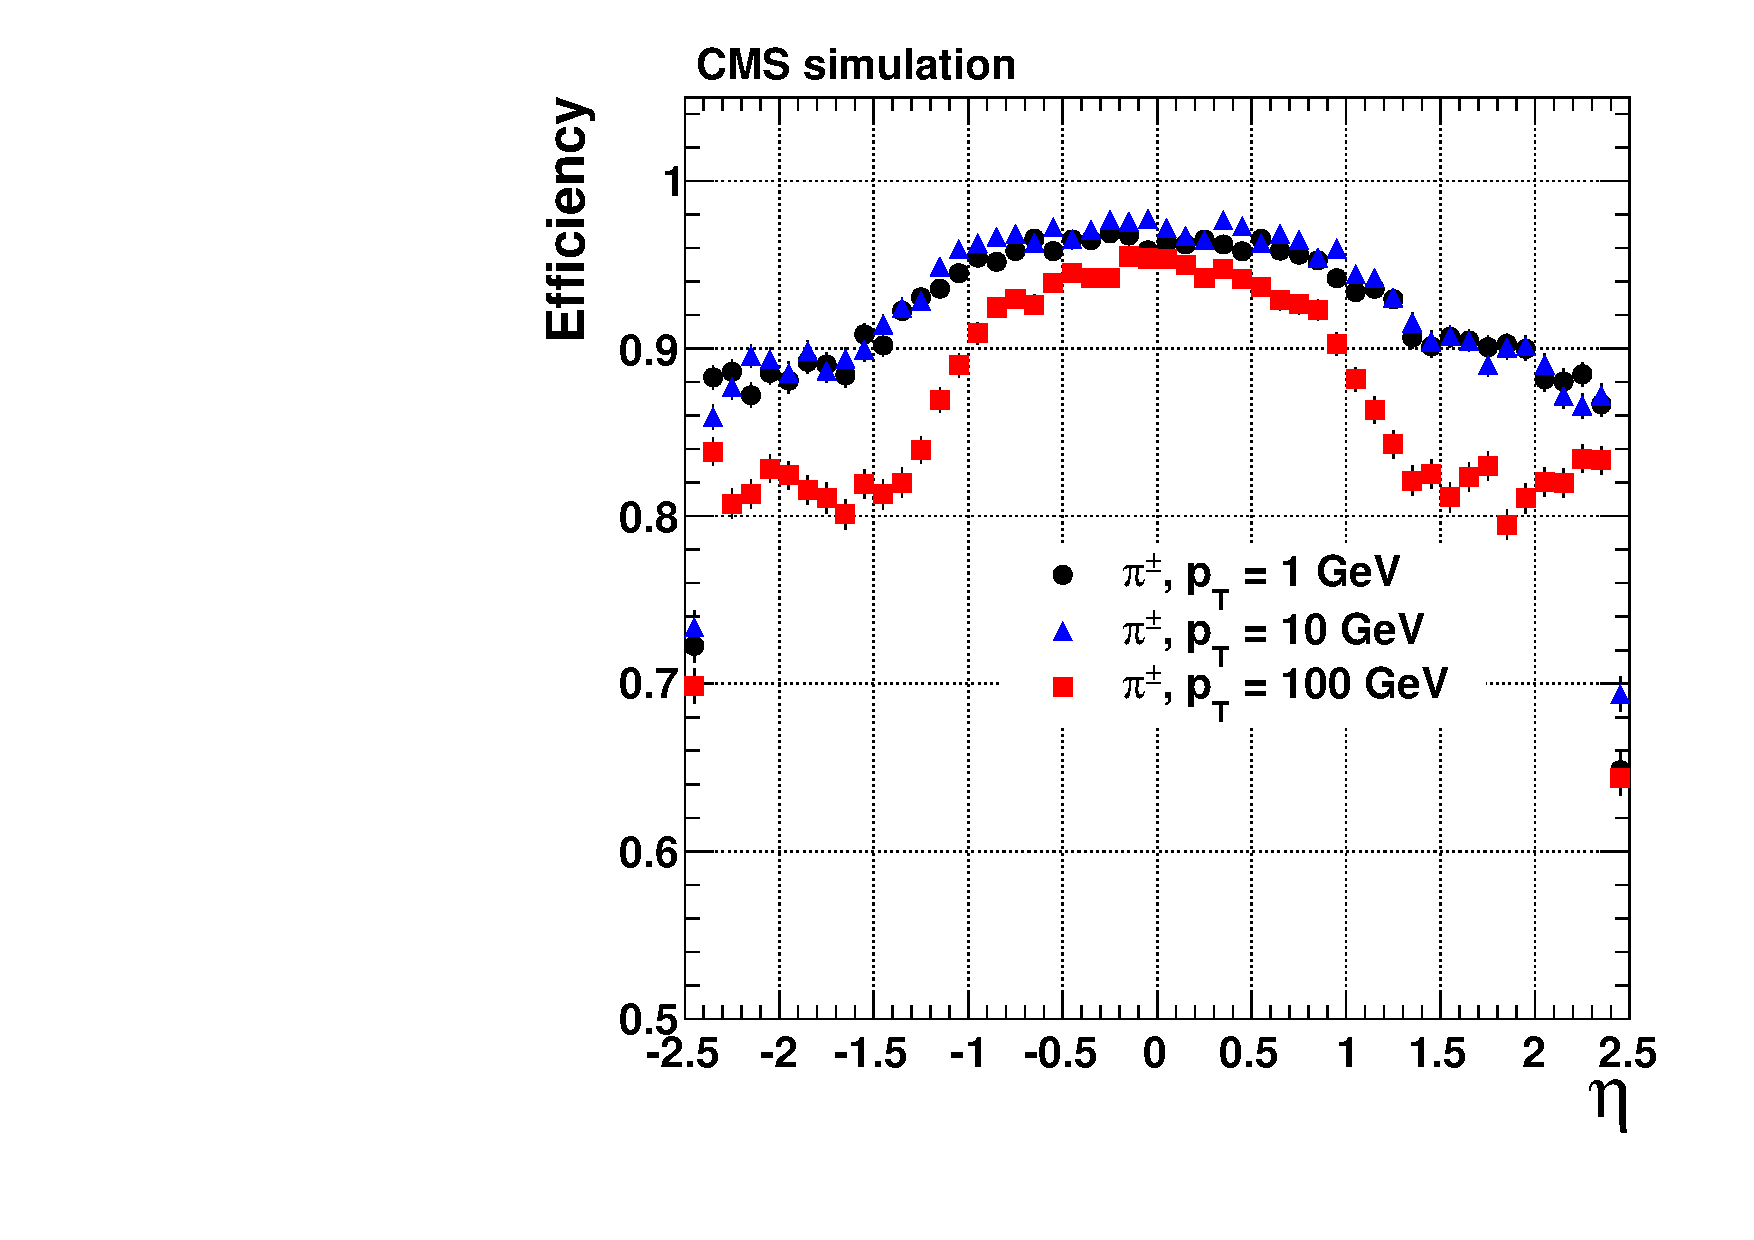
\includegraphics[width=0.30\textwidth]{\chsix/pi-efficiencyVsEta.pdf}}
\caption{Track reconstruction efficiency for simulated muons (a), electrons (b), and pions (c) passing the high-purity quality requirements as a function of $\eta$ and for \pt = 1, 10, and 100 \GeV~\cite{Chatrchyan:2014fea}.}
\label{fig:track_eff}
\end{figure}

\begin{figure}[!htb]
 \begin{center}
  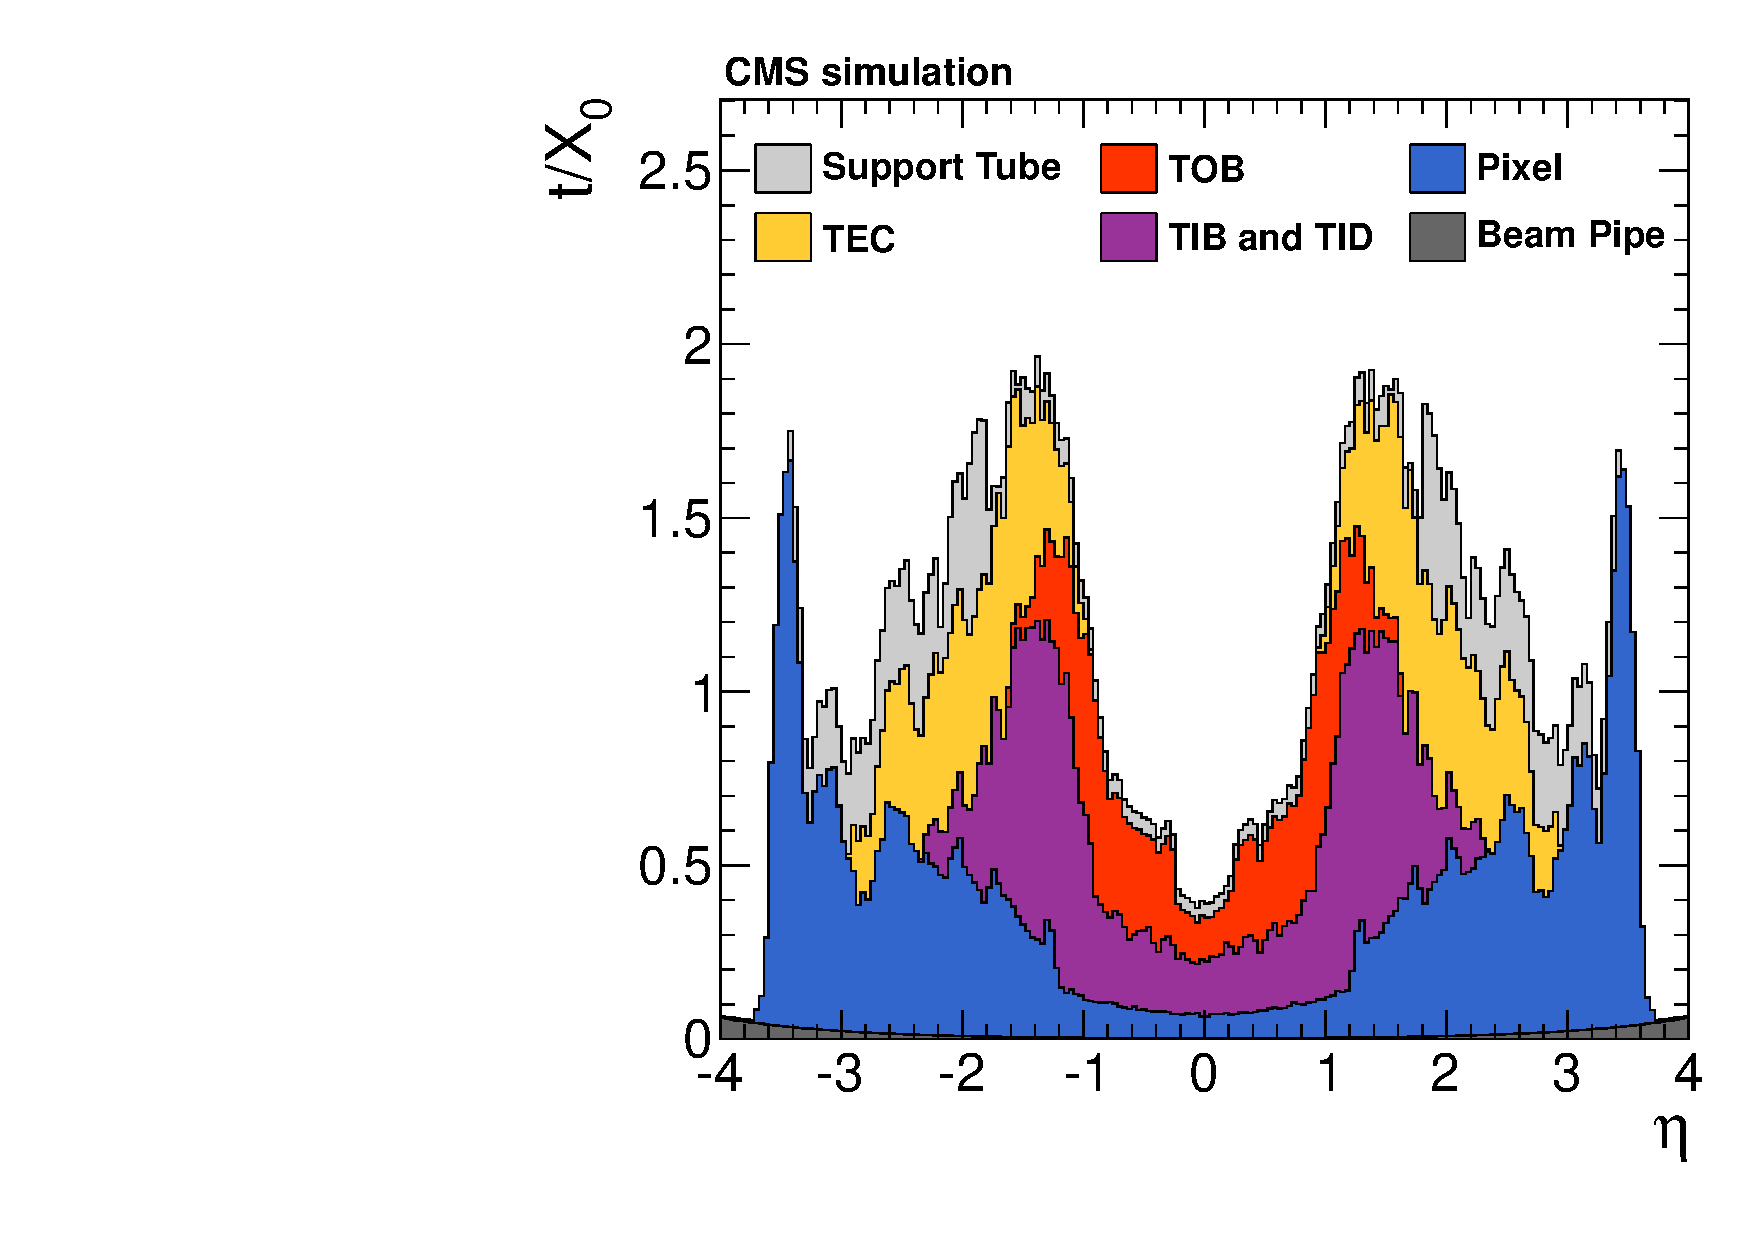
\includegraphics[width=0.45\textwidth]{\chsix/MaterialBudget_RadLengths.pdf}
 \end{center}
 \caption{Material budget of the CMS tracker in units of radiation length $X_0$ as a function of pseudorapidity divided into the contributions of the different subdetectors~\cite{Chatrchyan:2014fea}.}
 \label{fig:budgetCMStracker}
\end{figure}

In Fig.~\ref{fig:track_mu_rel_a} the transverse momentum resolution for muon tracks with $\pt$ = 1, 10 and 100\GeV is shown. At high transverse momentum (100\GeV), the resolution is 2--3\% up to $|\eta| = 1.6$.
%, but deteriorates at higher $|\eta|$ values, because of the shorter lever arm of these tracks in the $x$-$y$ plane of the tracker.
%The degradation at $|\eta| \sim 1.0$ and beyond is due to the gap between the barrel and the endcap disks, and due to the inferior hit resolution of the last hits of the track measured in TEC ring 7 compared to the hit resolution in TOB layers 5 and 6.
The material of the tracker accounts for 20--30\% of the transverse momentum resolution.
At lower momenta, the resolution is dominated by multiple scattering and its distribution reflects the amount of material traversed by the track.
The resolution of the track impact parameter in the transverse and longitudinal plane are also shown in Fig.~\ref{fig:track_mu_rel}. At high momentum the transverse impact parameter resolution is fairly constant and is dominated by the hit resolution in the first pixel layer. It is progressively degraded by multiple scattering at lower momenta. The same applies to the longitudinal impact parameter resolution. The improvement of the $z_0$ resolution up to $|\eta| = 0.5$ is due to the charge sharing effects among neighboring pixels.

\begin{figure}[!htb]
\centering
\subfigure[]{\label{fig:track_mu_rel_a}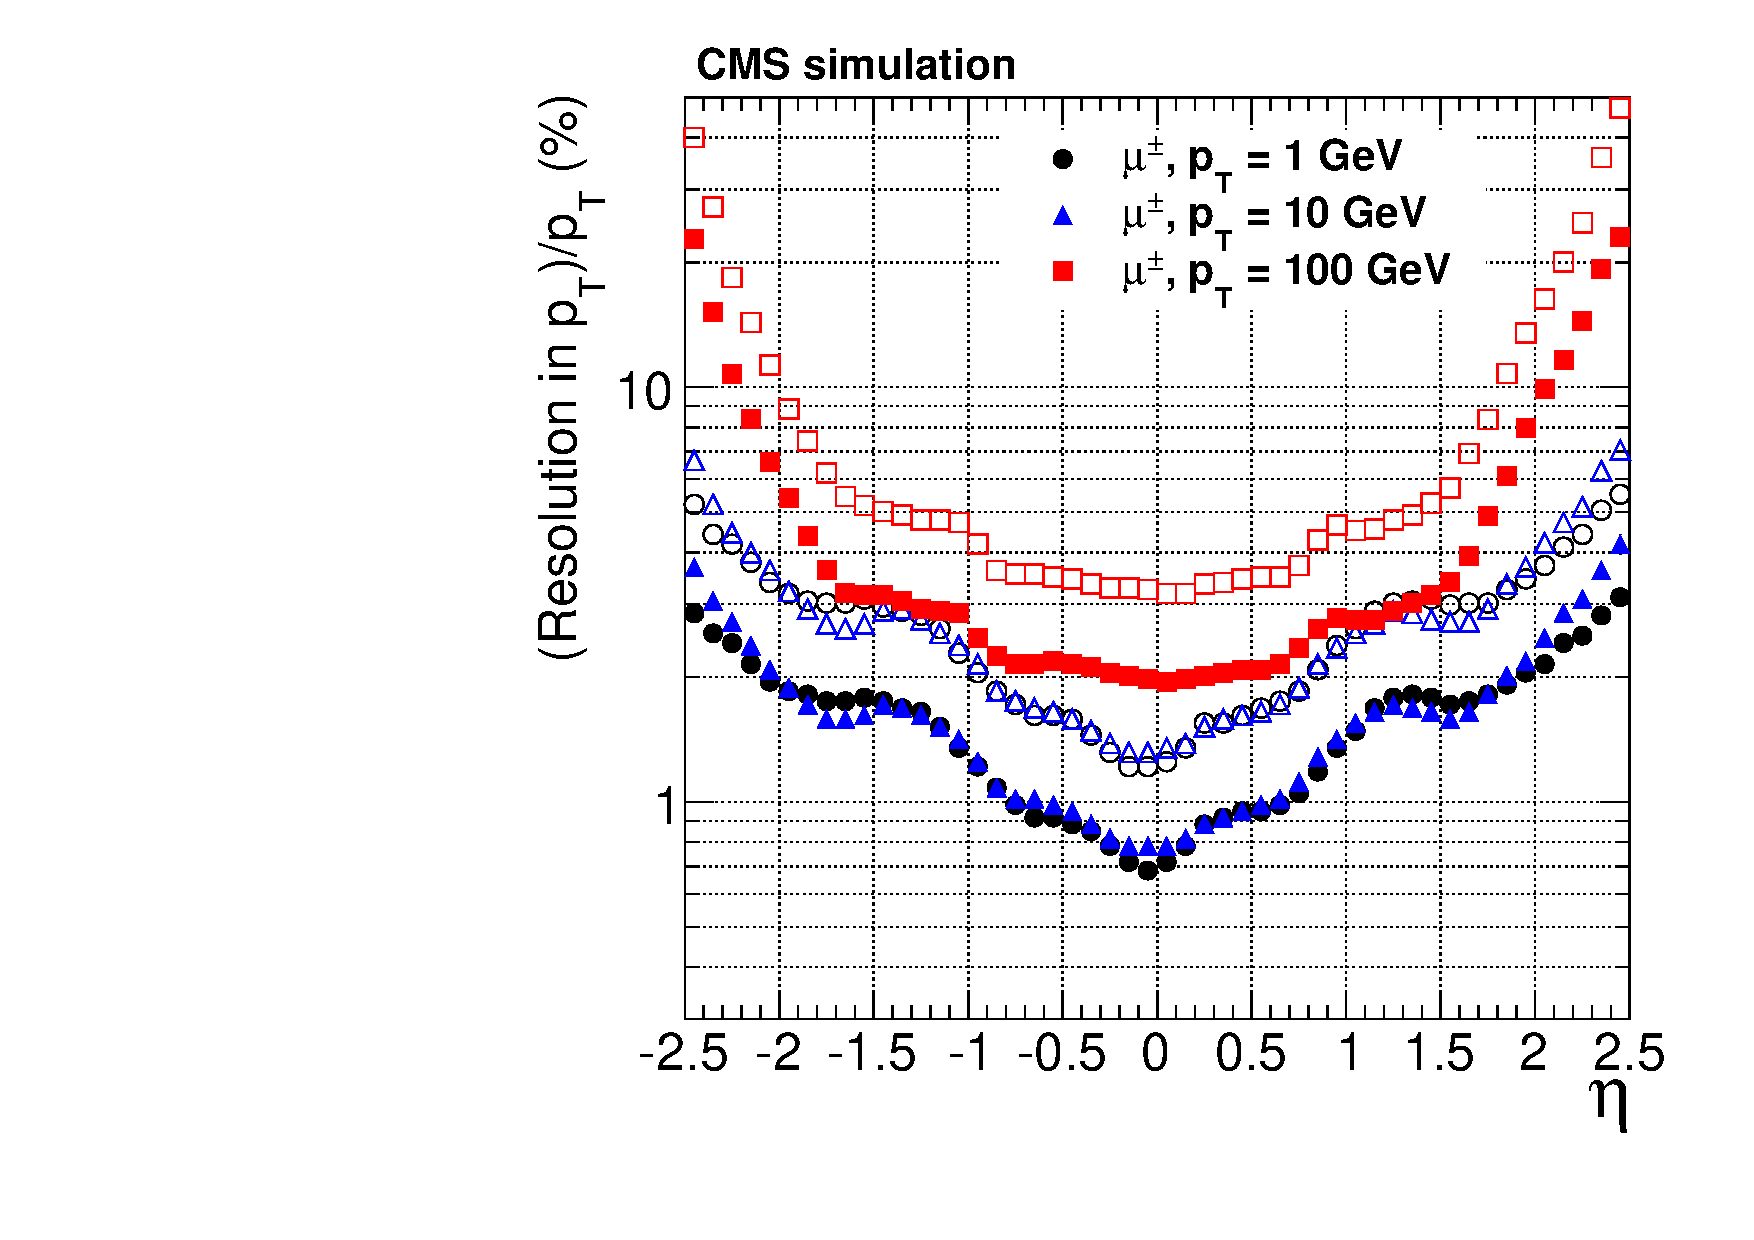
\includegraphics[width=0.30\textwidth]{\chsix/mu-resolutionPtVsEta.pdf}}
\subfigure[]{\label{fig:track_mu_rel_b}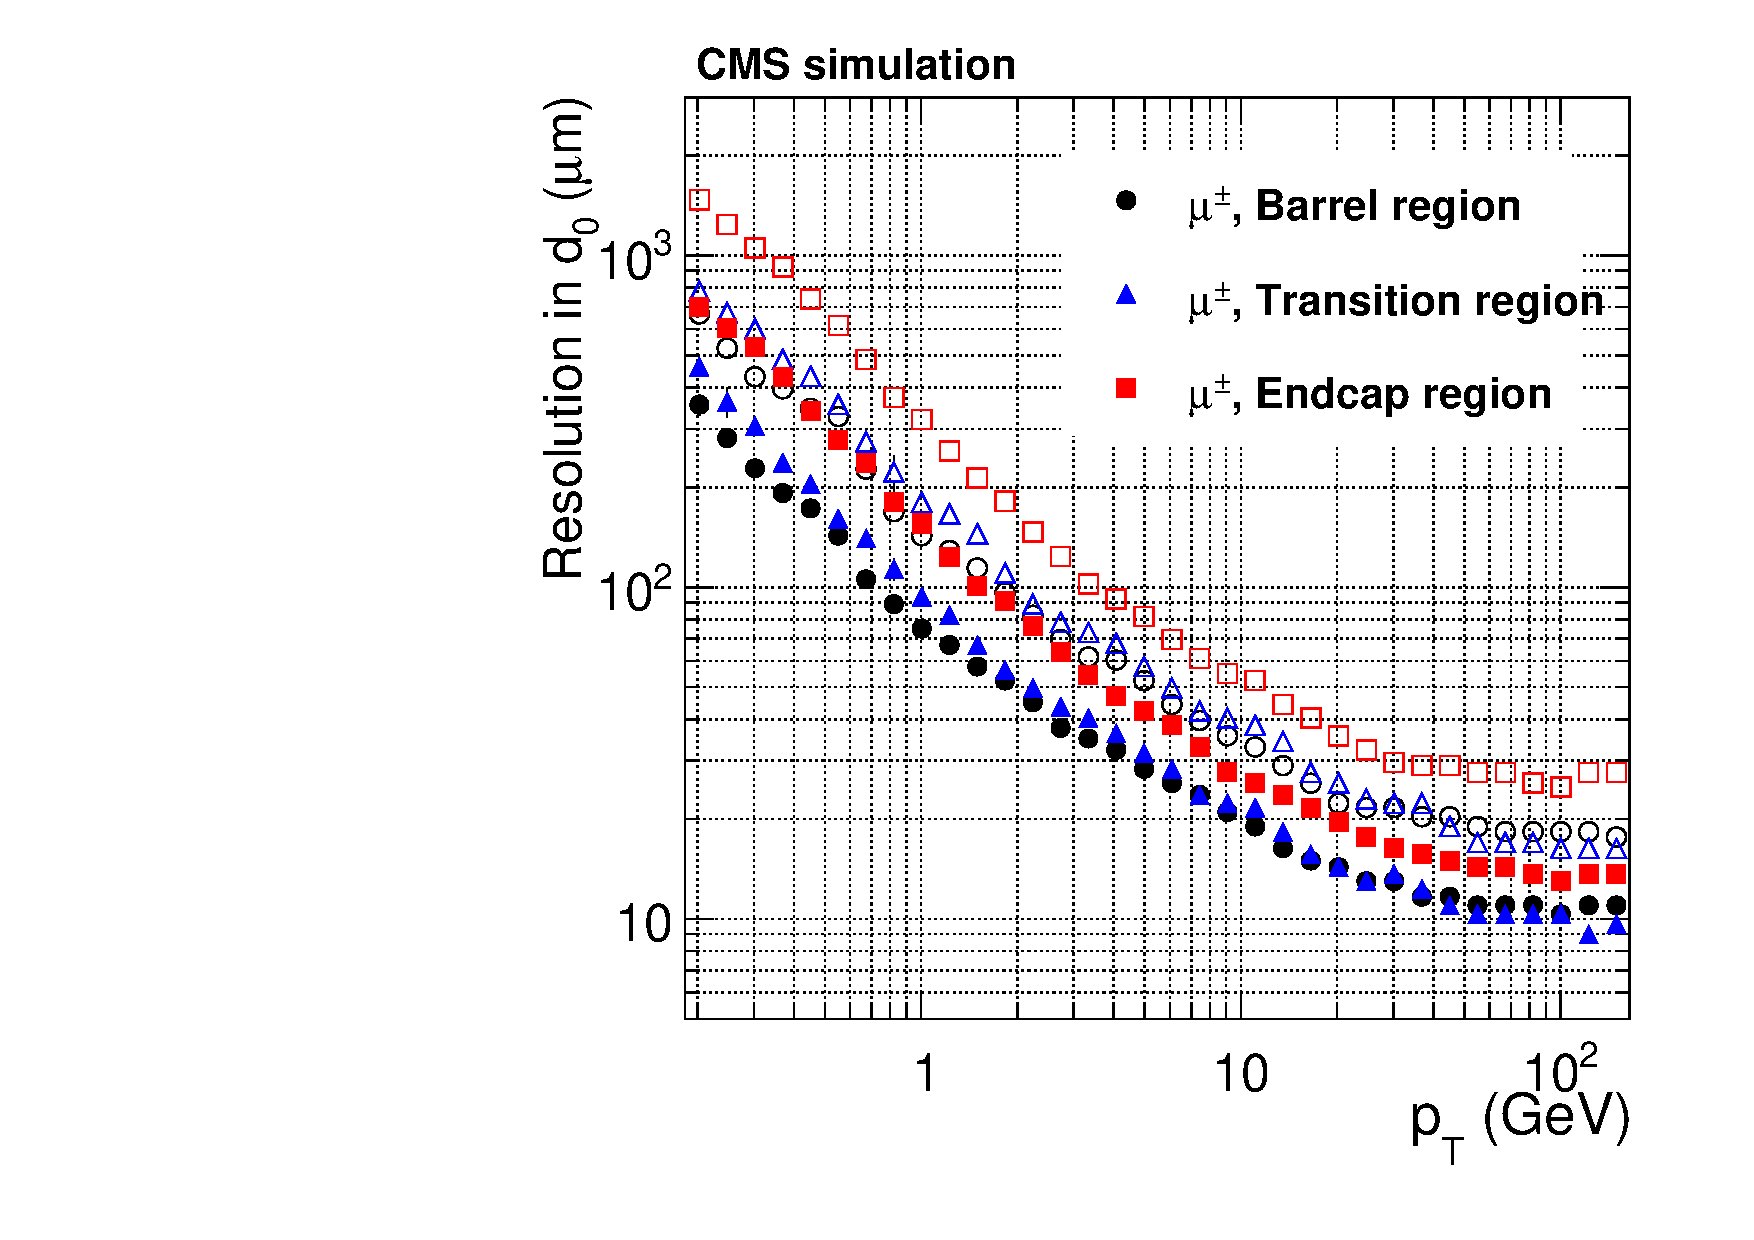
\includegraphics[width=0.30\textwidth]{\chsix/mu-resolutionD0VsPt.pdf}}
\subfigure[]{\label{fig:track_mu_rel_c}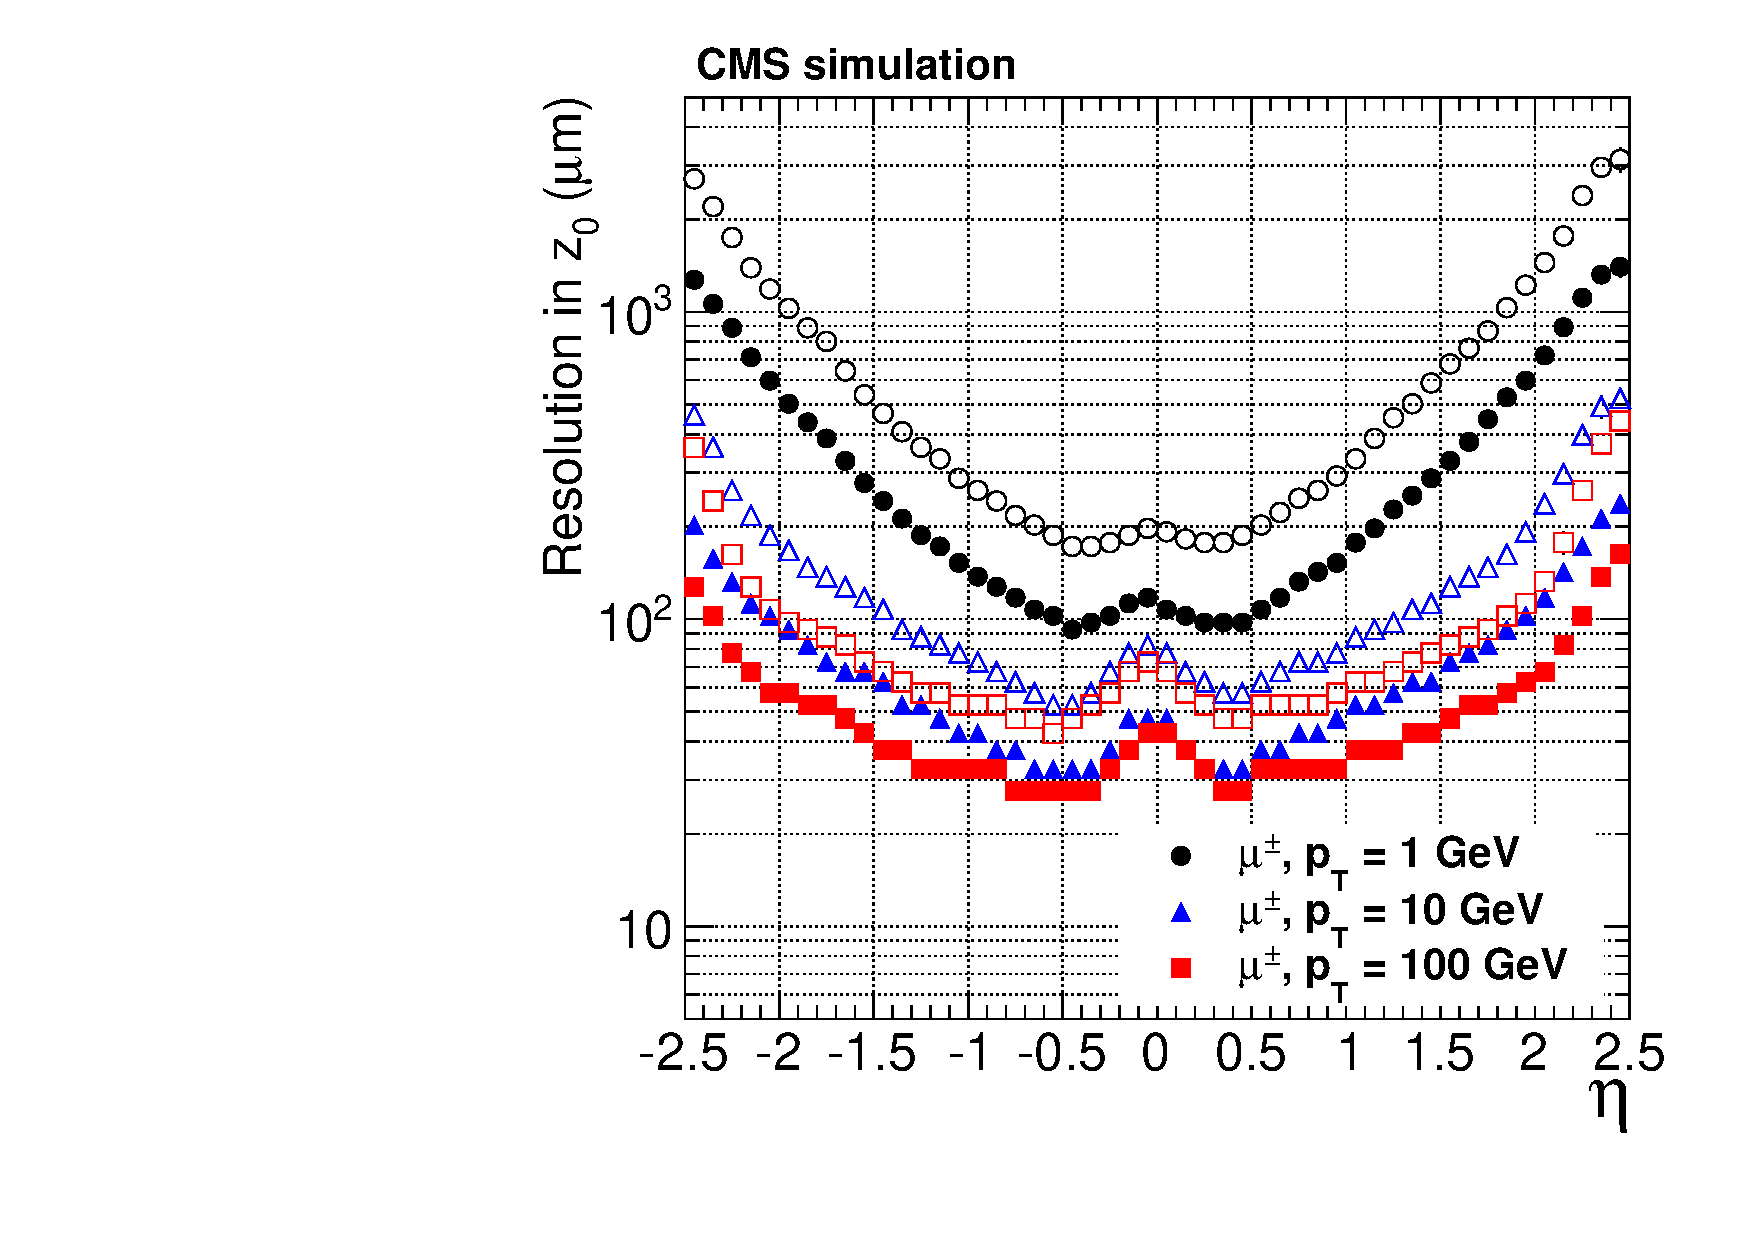
\includegraphics[width=0.30\textwidth]{\chsix/mu-resolutionDzVsEta.pdf}}
\caption{Resolution of track transverse momentum (a), transverse (b) and longitudinal (c) impact parameter for simulated muons passing the high-purity quality requirements as a function of $\eta$ and for \pt = 1, 10, and 100 \GeV~\cite{Chatrchyan:2014fea}.}
\label{fig:track_mu_rel}
\end{figure}

\subsection{Vertex reconstruction}

The identification of vertices is essential to distinguish the primary vertex associated with the hard interaction from additional pileup vertices that might be present in the event. This became even more important with the higher LHC luminosity reached at the end of 2016 where on average up to \FIXME{quote number} pp interactions took place simultaneously.

In the primary-vertex reconstruction~\cite{Speer:927395}, the measurements of the location and uncertainty of an interaction vertex are computed from a given set of reconstructed tracks. The prompt tracks originating from the primary interaction region are selected based on the transverse impact parameter significance with respect to the beam line, number of strip and pixel hits, and the normalized track $\chi^2$ from a fit to the trajectory. The selected tracks are then clustered on the basis of their $z$-coordinates at their point of closest approach to the centre of the beam spot using a {\itshape deterministic annealing} (DA) algorithm~\cite{726788}.
This clustering allows for the reconstruction of any number of proton-proton interactions in the same LHC bunch crossing. Vertices are resolved with separations about 1 mm, appropriate for a multiplicity of interactions per bunch crossing up to 20, as the longitudinal RMS spread of the luminous region is about 6 cm.

After identifying candidate vertices based on the DA clustering in $z$, those candidates containing at least two tracks are then fitted using an {\itshape adaptive vertex fitter}~\cite{0954-3899-34-12-N01} to compute the best
estimate of vertex parameters, including its $x$, $y$, and $z$ position and covariance matrix. This algorithm addresses the issue of secondaries and fake tracks in the cluster by iteratively down-weighting the tracks which are not compatible with the common vertex being fitted. The primary vertex originating the hard scattering is chosen as the vertex with highest sum of $\pt^2$ of the clustered tracks. The first vertex is usually the one corresponding to the collision of interest, where the hard process takes place.
%as well as the indicators for the success of the fit, such as the number of degrees of freedom for the vertex, and weights of the tracks used in the vertex. 

The primary vertex spatial resolution depends on the event topology and on the number of tracks related to the vertex, as shown in Fig.~\ref{fig:vtx_rel}. For minimum-bias events, the resolutions in $x$ and $z$ are, respectively, less than 20$\mu$m and 25$\mu$m, for primary vertices reconstructed using at least 50 tracks. The resolution is better for the jet-enriched sample where tracks have significantly higher mean \pt resulting in higher resolution in the track impact parameter and consequently better vertex resolution. For these events, the resolutions approach 10$\mu$m in $x$ and 12$\mu$m in $z$ for primary vertices using at least 50 tracks.

\begin{figure}[!htb]
\centering
\subfigure[]{\label{fig:vtx_rel_a}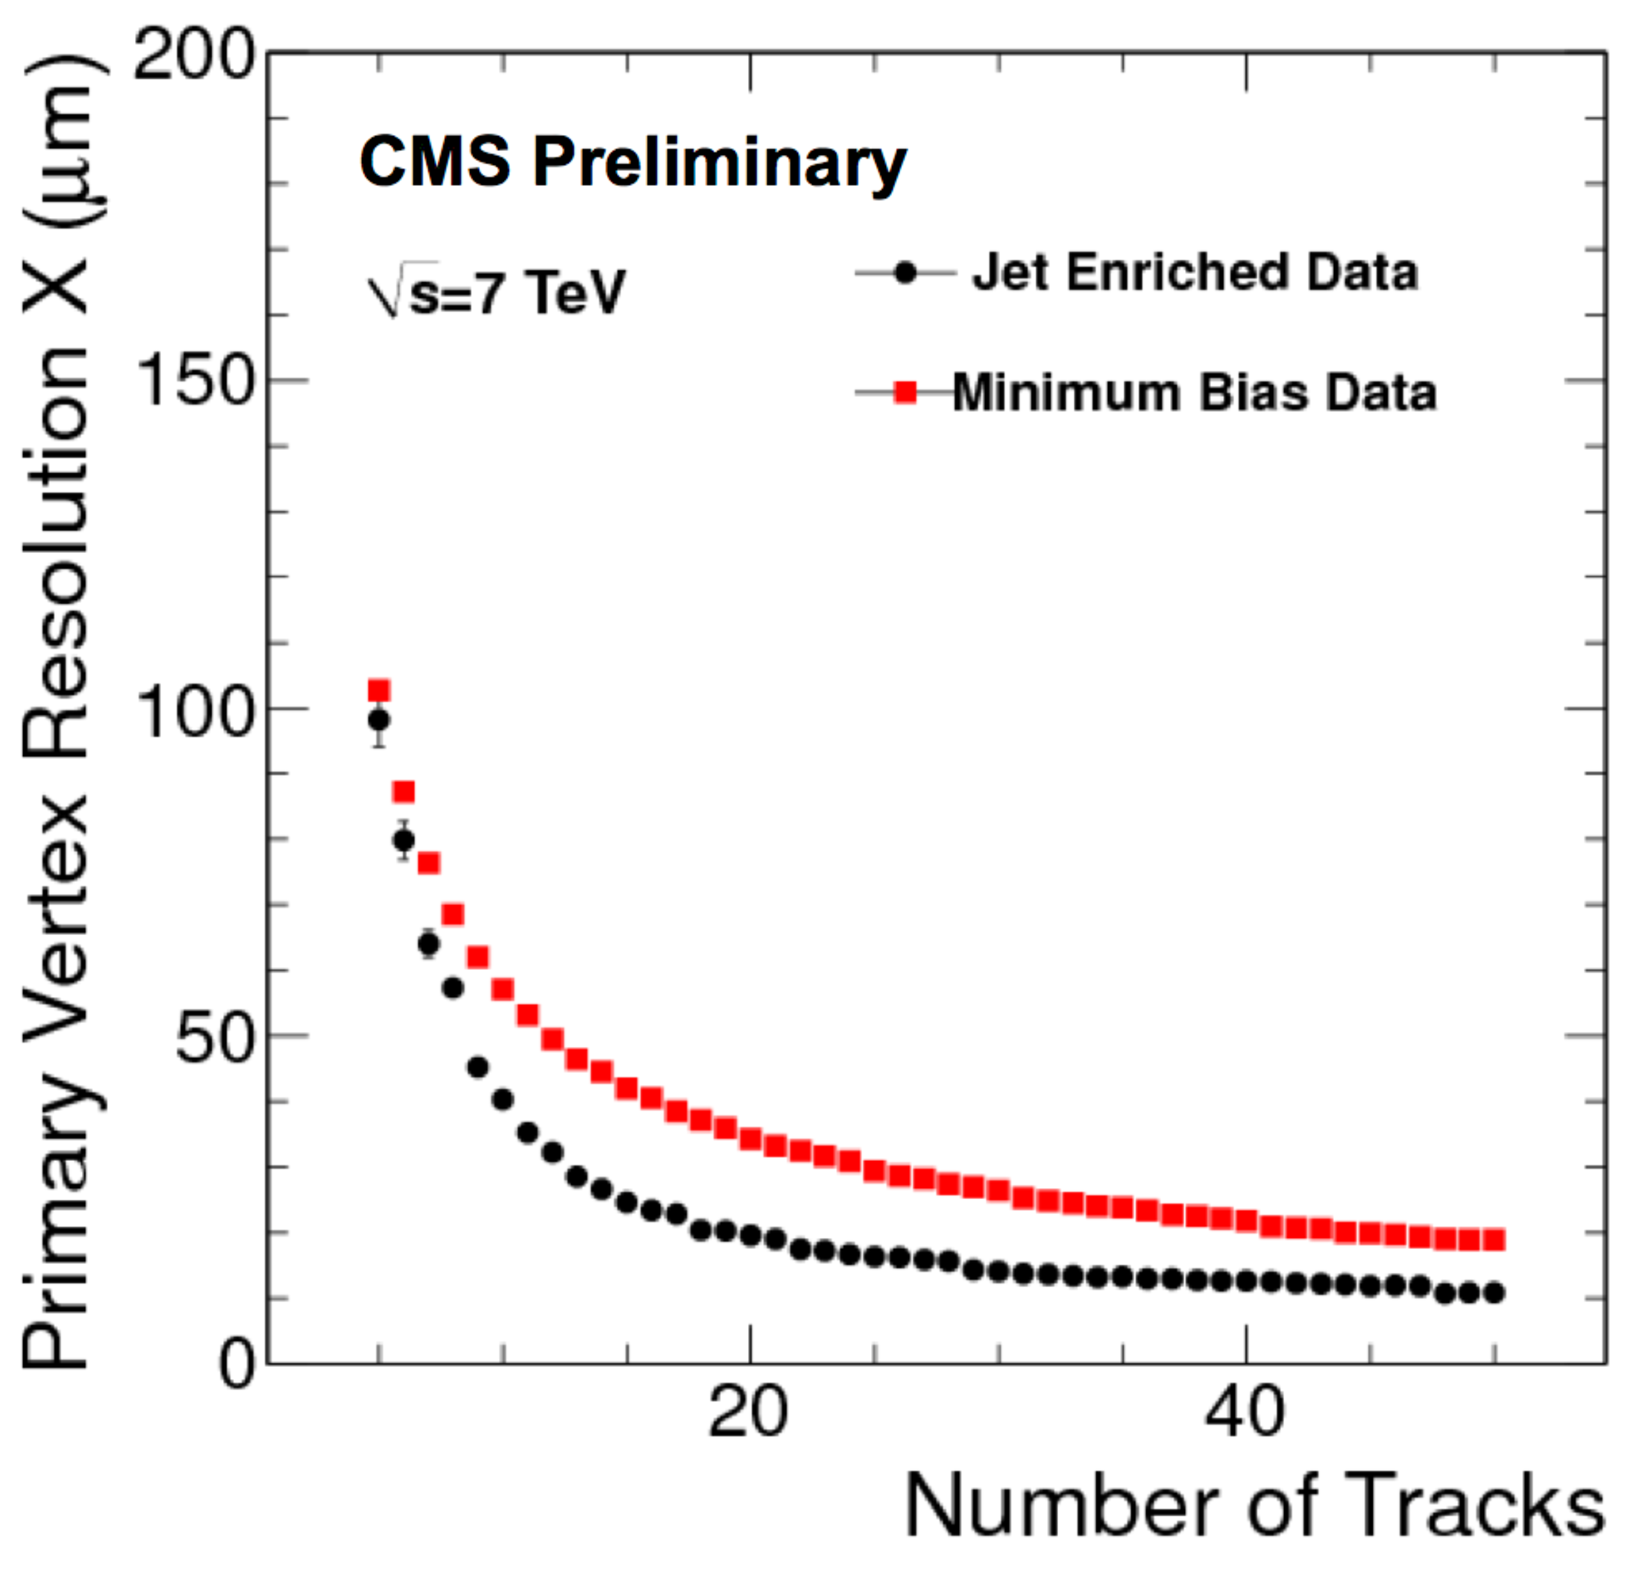
\includegraphics[width=0.45\textwidth]{\chsix/PrimaryVertexResolutionsX.pdf}}
\subfigure[]{\label{fig:vtx_rel_b}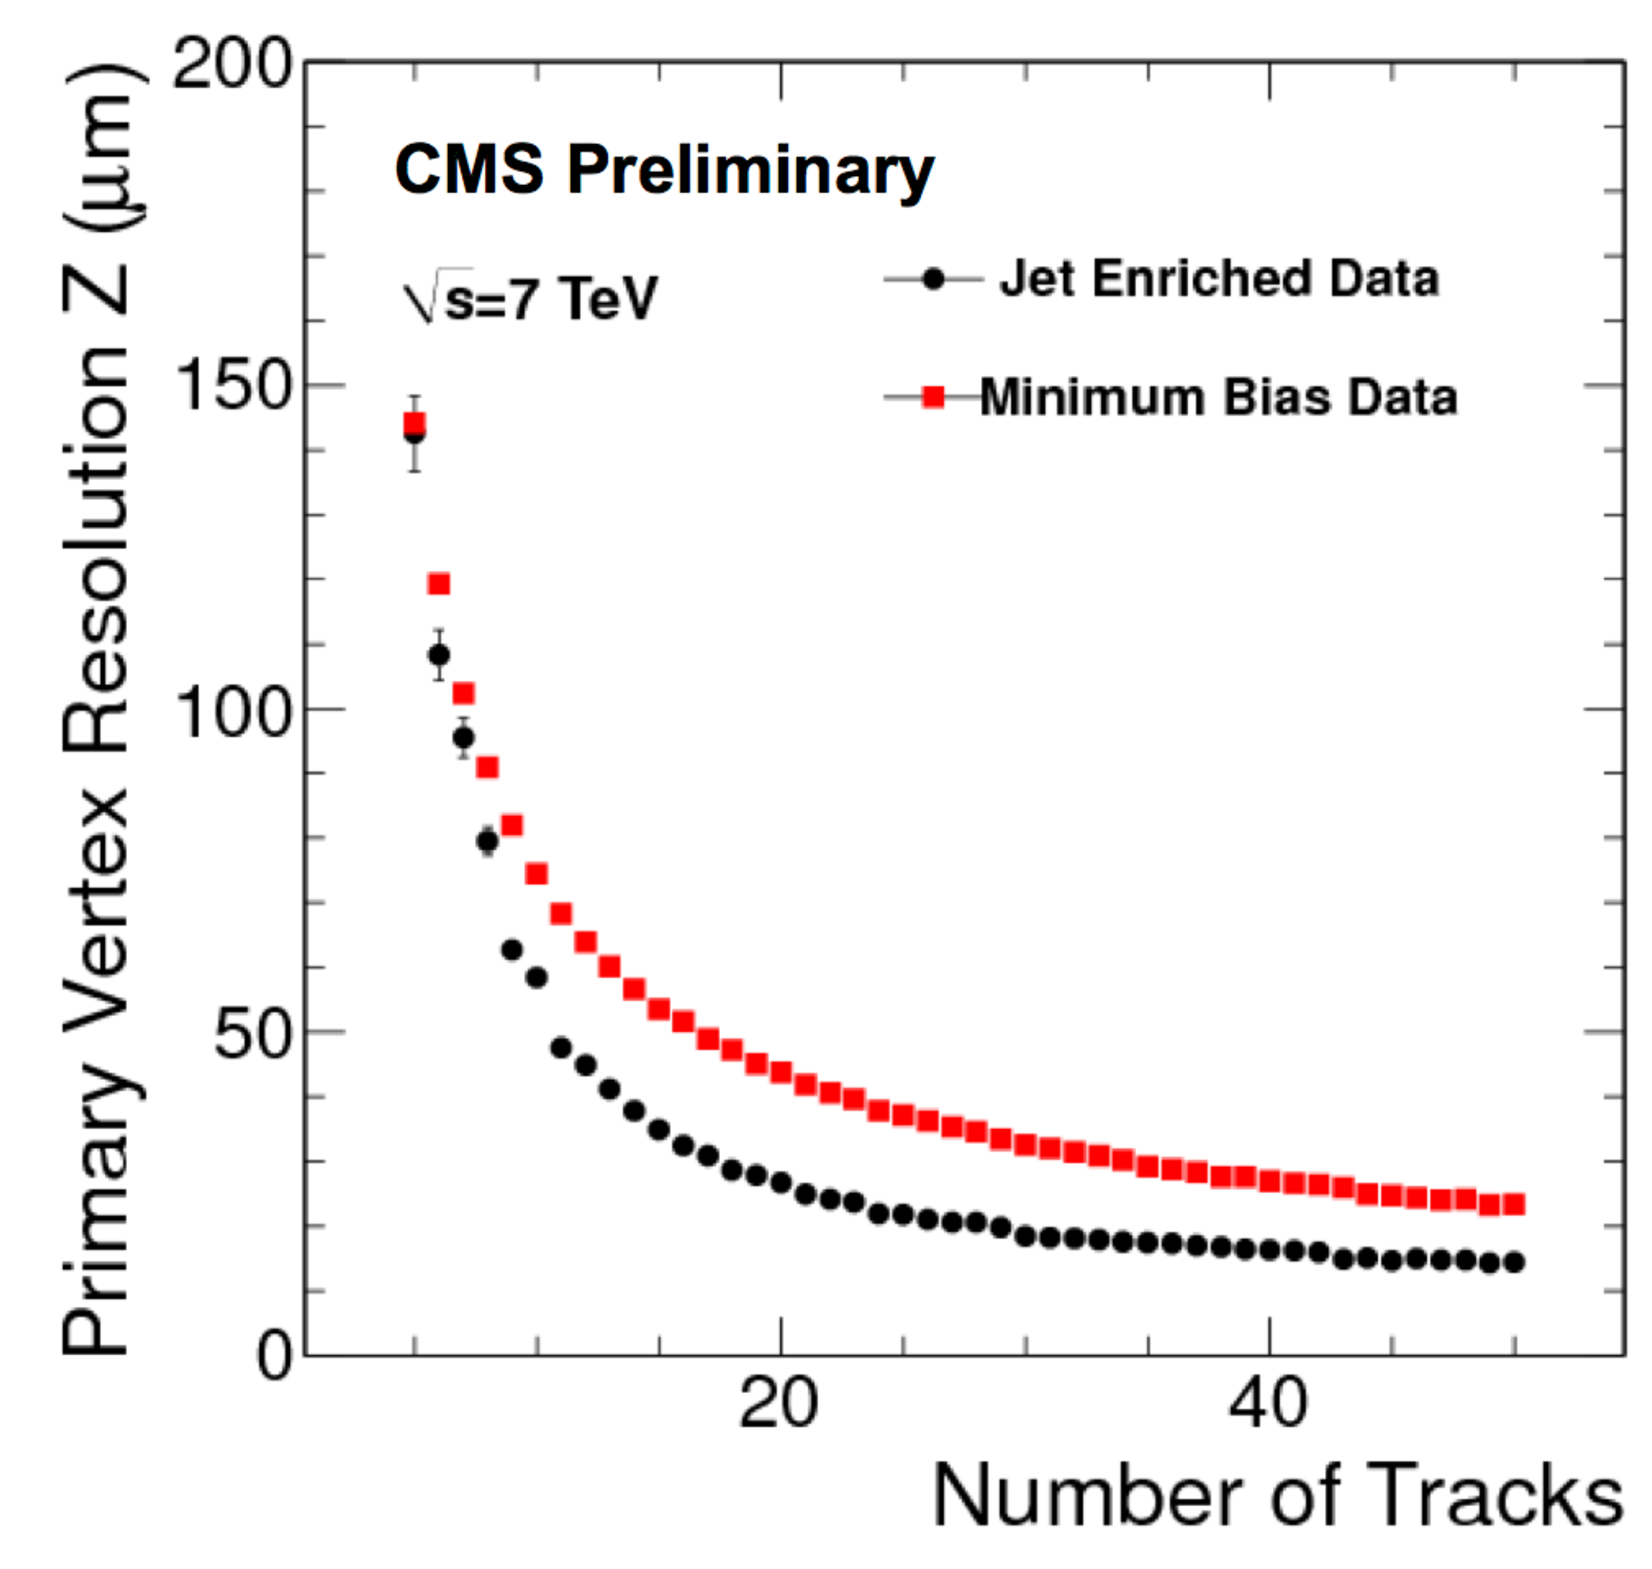
\includegraphics[width=0.45\textwidth]{\chsix/PrimaryVertexResolutionsZ.pdf}}
\caption{Primary-vertex resolution in $x$ (a) and $z$ (b) as a function of the number of tracks at the fitted vertex, for two kinds of events with different average track \pt values; the results in $y$ is almost identical to the one in $x$~\cite{TrkCMSPublicResults}.}
\label{fig:vtx_rel}
\end{figure}
 
%%%%%%%%%%
%\section{Electrons}\label{sec:electrons}
 %%%%%%%%%%%%%%%%%%%%%%%%%%%%%%%%%%%%%%%%%%%%%%%%%%%%%%%%%%%%%%%
\section{Electrons}\label{sec:electrons}
%%%%%%%%%%%%%%%%%%%%%%%%%%%%%%%%%%%%%%%%%%%%%%%%%%%%%%%%%%%%%%%
%
%%%%%%%%%%
\subsection{Electron reconstruction}\label{subsec:elereco}
%%%%%%%%%%

The electron reconstruction in CMS~\cite{Baffioni:2006cd} is based on the association of an energy deposit in the ECAL with a track reconstructed in the silicon tracker system.
Electrons lose energy primarily through bremsstrahlung when interacting with the tracker layers, and consequently they suffer from large energy losses.
Given the non-Gaussian properties of the energy loss distributions, the standard track reconstruction algorithm based on the KF is not appropriate
and leads in general to a reduced hit-collection efficiency, as well as to a poor estimation of track parameters. 
A better performance for electron reconstruction is achieved by using dedicated techniques that make use of information, not only from the tracker, but also from the ECAL, as described in the following.\\
%As electrons lose energy primarily through bremsstrahlung, large energy losses are common.
%About 35\% of electrons radiate more than 70\% of their initial energy before reaching ECAL.
%An important property of the electrons is their high probability of emitting a bremsstrahlung photon after interacting with one of the tracker layers.
%Electrons, being charged particles, can be reconstructed through the standard track reconstruction.  However,  as electrons lose energy primarily through bremsstrahlung,  rather than ion- ization,  large energy losses are common.  For example,  about 35\% of electrons radiate more than 70\% of their initial energy before reaching the electromagnetic calorimeter (ECAL) that surrounds the tracker.  The energy loss distribution is highly non-Gaussian, and therefore the standard Kalman filter, which is optimal when all variables have Gaussian uncertainties, is not appropriate. As a result, the efficiency and resolution of the standard tracking are not particularly good for electrons and therefore electron candidates are reconstructed using a combination of two techniques that make use of information, not only from the tracker, but also from the ECAL. 

The electron reconstruction starts by searching for clusters of energy in the ECAL.
As the electrons are degraded in energy, the effect of the magnetic field is to enhance the bending of their trajectories, resulting in a spread of irradiated photons along the $\phi$ coordinate.
To recover this radiated energy, ECAL superclusters are formed, by merging clusters of similar $\eta$ over some range of $\phi$.
Because of the different geometry of the detector in barrel and endcap, different clustering algorithms are used in different regions.
%Because of bremsstrahlung the electron energy usually spreads out over several crystals of the ECAL. 
%Bremsstrahlung photons emitted by the electrons strike, in general, the ECAL at $\eta$ values similar to that of the electron,
%but at different $\phi$. To recover this radiated energy, ECAL superclusters are formed, by merging clusters of similar $\eta$ over some range of $\phi$.
%Because of the different geometry of the detector in barrel and endcap, different clustering algorithms are used in different regions
%The first method [35] starts by searching for clusters of energy in the ECAL. The curvature
%of electrons in the strong CMS magnetic field means that bremsstrahlung photons emitted by
%the electrons will, in general, strike the ECAL at eta values similar to that of the electron, but
%at different azimuthal coordinates phi.  To recover this radiated energy, ECAL superclusters
%are formed, by merging clusters of similar eta over some range of f.  

For the electron track reconstruction two approaches are used.
In the first one, referred to as ``ECAL driven'', the supercluster energy and position, and the assumption that the electron originated near the center of the beam spot, are used to extrapolate the electron trajectory in the tracker. Tracker seeds compatible with the predicted trajectory are sought in the first or second layer of the pixel detector (and also in the TEC to improve efficiency in the forward region).
This method is designed for isolated electrons with $\pt > 5\GeV$.

%A ?tracker driven? approach, developped in the context of the PF algorithm, is also used and extends the electron track reconstruction for low momentum and non isolated electrons.
A second approach, referred to as ``tracker driven'', complements the electron track reconstruction,
especially for low-\pt or non isolated electrons, as well as for electrons in the barrel-endcap transition region. This method is developed as part of the particle-flow (PF) reconstruction algorithm~\cite{CMS-PAS-PFT-10-001,CMS-PAS-PFT-09-001} described in Section~\ref{subsec:jetsreco}.
It takes the standard track collection reconstructed with the KF algorithm and attempts to identify a subset of these tracks that are compatible with being electrons. 
Electrons that suffer only little bremsstrahlung loss can be identified by searching for tracks extrapolated to the ECAL that pass close to an ECAL PF cluster.
Electrons that suffer large bremsstrahlung loss can be identified by the fact that the fitted track will often have poor $\chi^2$ or few associated hits. 
The track seeds originally used to generate these electron-like tracks are retained.

The seed collections obtained by using these two methods are merged, and used to initiate electron track finding. 
This procedure is similar to that used in standard tracking, except that the $\chi^2$ threshold, used by the KF to decide whether a hit is compatible with a trajectory, is weakened. 
This is to accommodate tracks that deviate from their expected trajectory because of bremsstrahlung.

To obtain the best estimate of the track parameters, the final track fit is performed using a modified version of the KF method, called the Gaussian Sum Filter (GSF)~\cite{0954-3899-31-9-N01}.
The fractional energy loss of an electron, as it traverses a layer of material, follows a Bethe--Heitler distribution. 
This distribution is non-Gaussian, making it unsuitable for use in a conventional KF algorithm. 
The GSF technique solves this by approximating the Bethe--Heitler energy-loss distribution as the sum of several Gaussian  functions.
This method is then a generalization of the KF where the trajectory in each tracker layer is described by a weighted sum of KF components for which the energy loss follows a Gaussian law with a given width.
The propagation of each component is done separately from one layer to another and the weights are then updated given the measurement in the new site.
The allowed window to search for a hit in the next tracker layer is larger than for the usual KF track.
This procedure is iterated until the last tracker layer, unless no hit is found in two subsequent layers. A minimum of five hits is finally required to create a track.
A GSF electron candidate is finally built by associating an ECAL supercluster with a GSF track with compatible $\eta$ and $\phi$ positions.

The electron transverse energy \et is equal to the transverse energy of the correspondent ECAL energy deposit (or supercluster) $\et^\mathrm{SC}$, and defined as
$\et = E\sin\theta$, where $\theta$ is the polar angle of the supercluster (ST) relative to the beam axis,
and $E$ the energy measured in the supercluster. 

The performance of the GSF electron reconstruction are studied using a ``tag-and-probe'' (T\&P) method~\cite{Khachatryan:2010xn}.
The method uses a known SM resonance mass and decay (e.g. $\PZ\to\EE$) to select particles of the desired type and probe the efficiency of a particular selection criterion on those particles. In general the ``tag'' is an object that passes a set of very tight selection criteria designed to isolate the required particle type (in this case an electron, though the method is not strictly limited to this case). A generic set of the desired particle type (i.e. with potentially very loose selection criteria) known as ``probes'', is selected by pairing these objects with tags such that the invariant mass of the combination is consistent with the mass of the resonance. Combinatoric backgrounds are usually eliminated through a variety of background subtraction methods. The definition of the probe object depends on the specifics of the selection criterion being examined. The efficiency itself is measured by counting the number of ``probe'' particles that pass the desired selection criteria. It is found that the estimated efficiencies are almost insensitive to any specific definition of the tag. 
%which exploits Z/$\gamma^*\rightarrow$e$^+$e$^-$ events in data to estimate the reconstruction and selection efficiencies for signal electrons. The method requires one electron candidate, called the ``tag'', to satisfy tight selection requirements. Different criteria are tried to define the tag electron, and it is found that the estimated efficiencies are almost insensitive to any specific definition of the tag. 
The GSF electron reconstruction efficiency measured with this method is above 95\% for electrons in the ECAL barrel with $\et > 35\GeV$, as shown in Fig.~\ref{fig:el_reco_a}. Slightly lower efficiencies are obtained for electrons reconstructed in the ECAL endcaps (Fig.~\ref{fig:el_reco_b}). A good agreement is found between data and simulation, resulting in scale factors consistent with unity almost in the entire range. The performance are presented here for the electron reconstruction in Run~1 but similar results are obtained in CMS for Run~2.\\

\begin{figure}[!htb]
\centering
\subfigure[]{\label{fig:el_reco_a}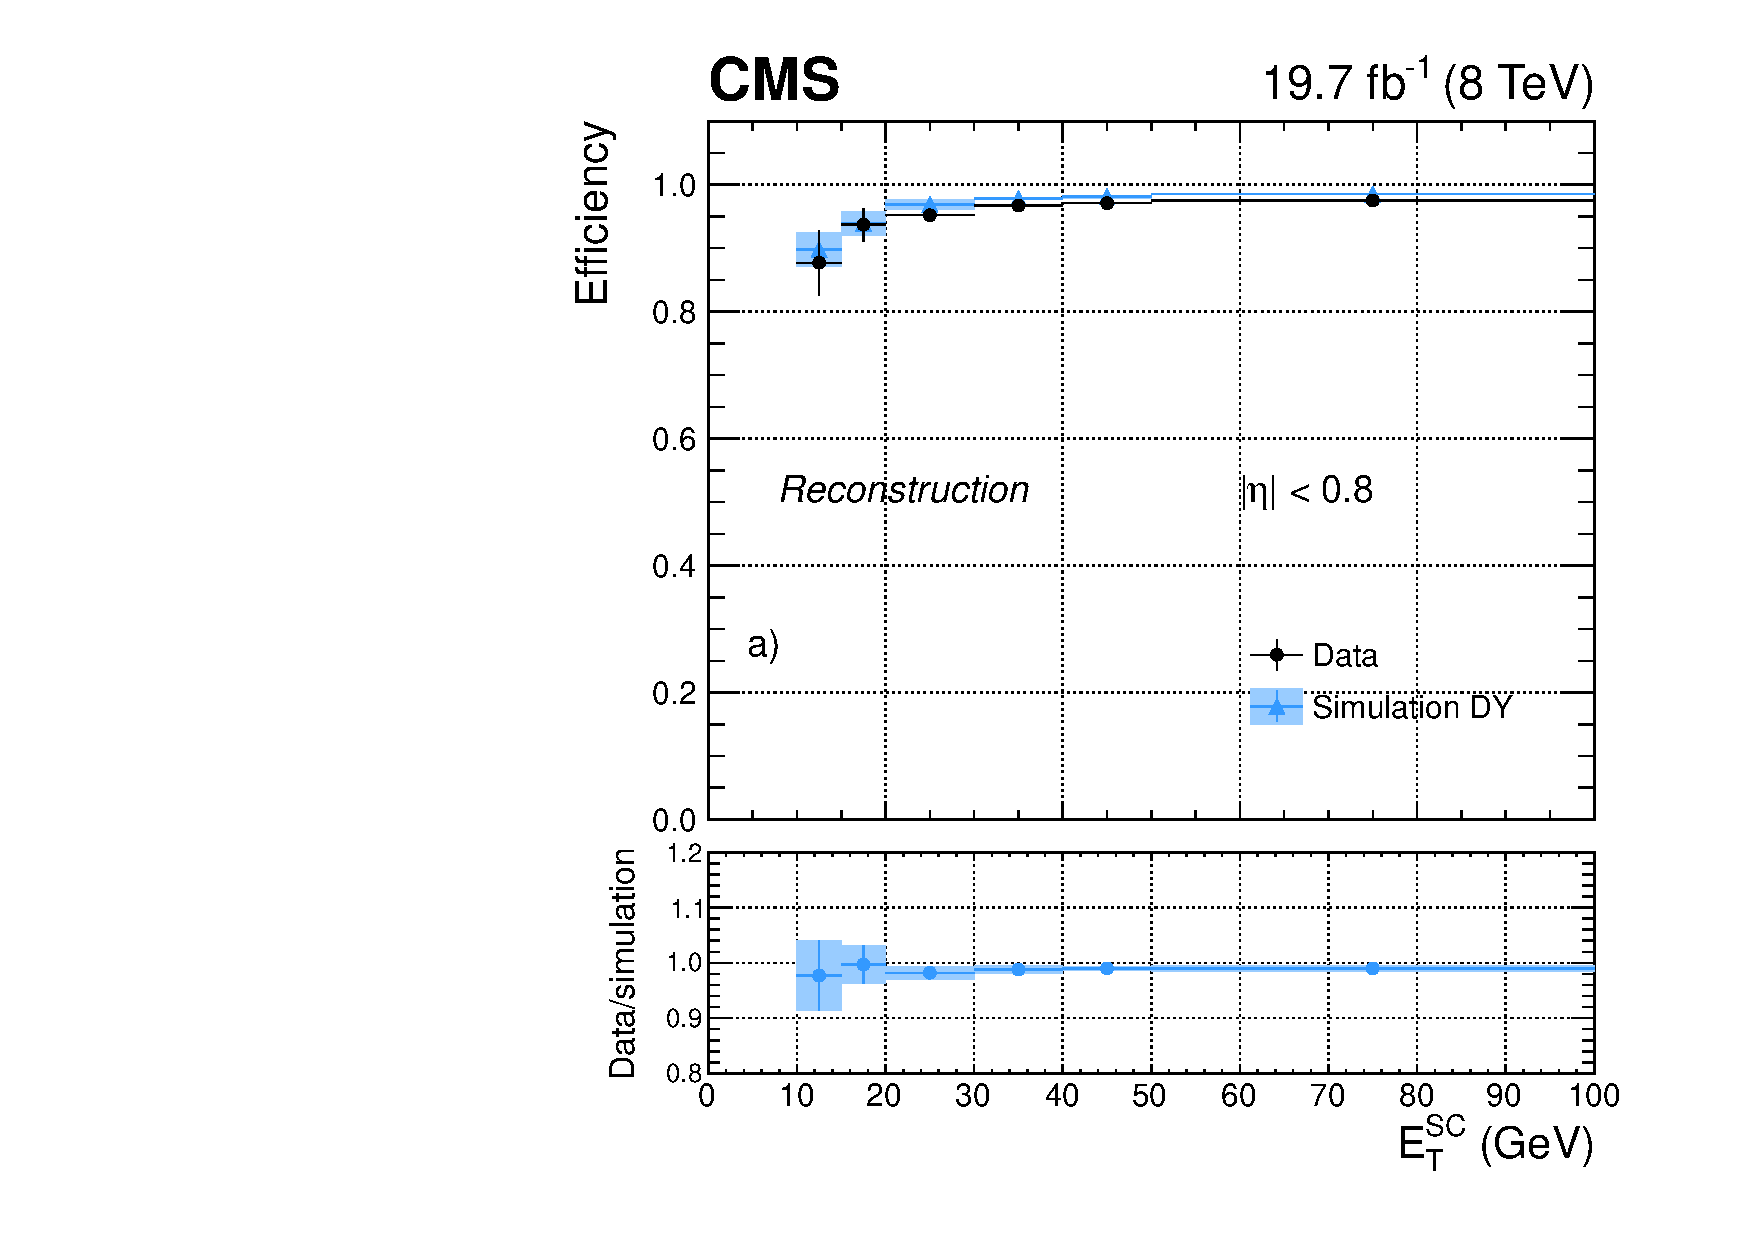
\includegraphics[width=0.45\textwidth]{\chsix/ele-reco-eff-eta-bin-0.pdf}}
\subfigure[]{\label{fig:el_reco_b}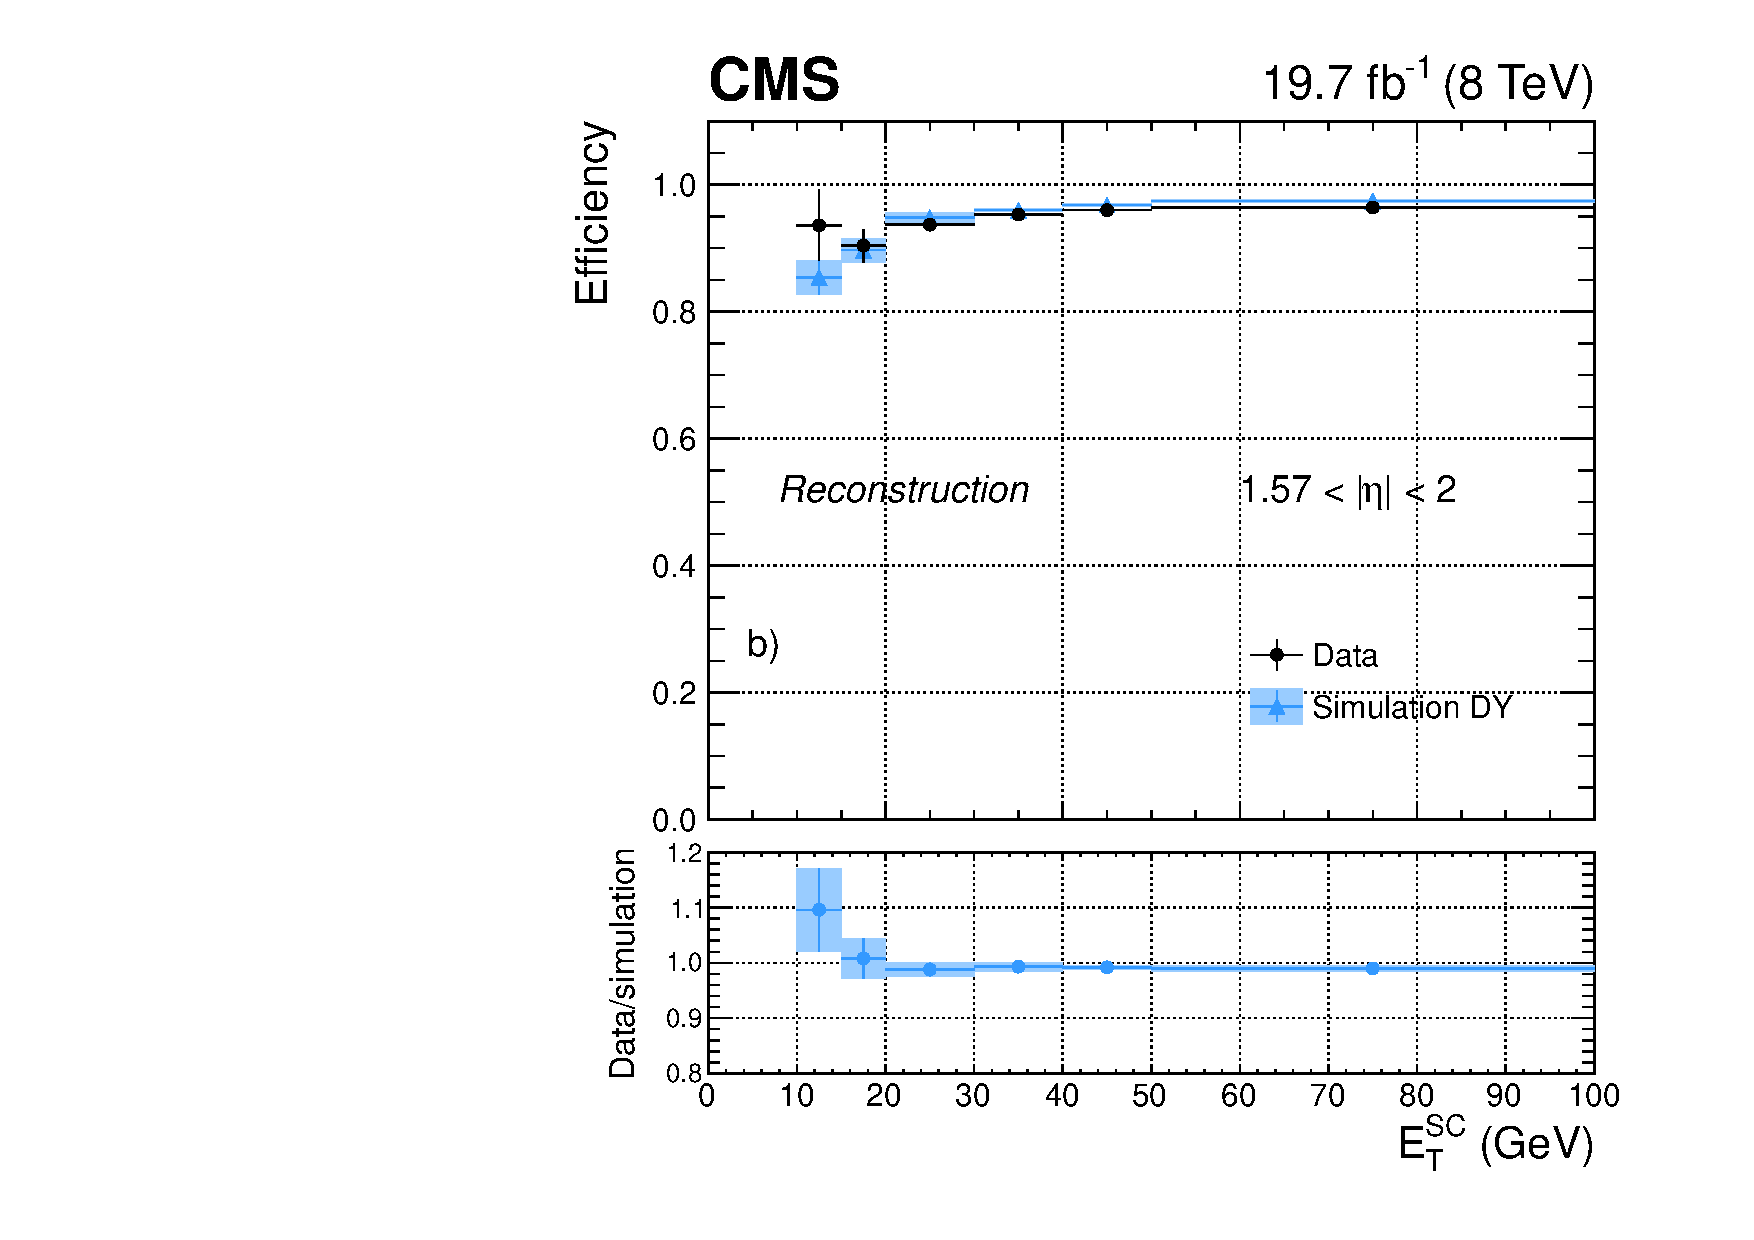
\includegraphics[width=0.45\textwidth]{\chsix/ele-reco-eff-eta-bin-3.pdf}}
\caption{Electron reconstruction efficiency measured in dielectron events in data (dots) and Drell-Yan simulation (triangles), as a function of the \et
for electrons reconstructed in the ECAL barrel (a) and endcaps (b). The bottom panels show the corresponding data-to-simulation scale factors~\cite{Khachatryan:2015hwa}.
%The uncertainties shown in the plots correspond to the quadratic sum of the statistical and systematic contributions~\cite{Khachatryan:2015hwa}.
}
\label{fig:el_reco}
\end{figure}

Once a GSF electron candidate is reconstructed, the energy measurement provided by electromagnetic calorimeter can be combined with the tracker momentum measurement to improve the estimate of electrons with energies below 35\GeV as shown in Fig.~\ref{fig:eleres}.
%For medium and low energy values ($< 35\GeV$), the momentum is obtained as a weighted sum of the supercluster energy and track momentum measurements.
At energies above 35\GeV however, the momentum measurement is completely driven by the supercluster.
%The energy measurement provided by electromagnetic calorimeter can be combined with the tracker momentum measurement to improve the estimate of the electron momentum for low energy particles. The improvement is expected to come both from the opposite behaviour with E or p of the intrinsic calorimetry and tracking resolutions, and from the fact that ptk and Esc are differently affected by the bremsstrahlung radiation (see Figure 2.12).

\begin{figure}[!htb]
 \begin{center}
  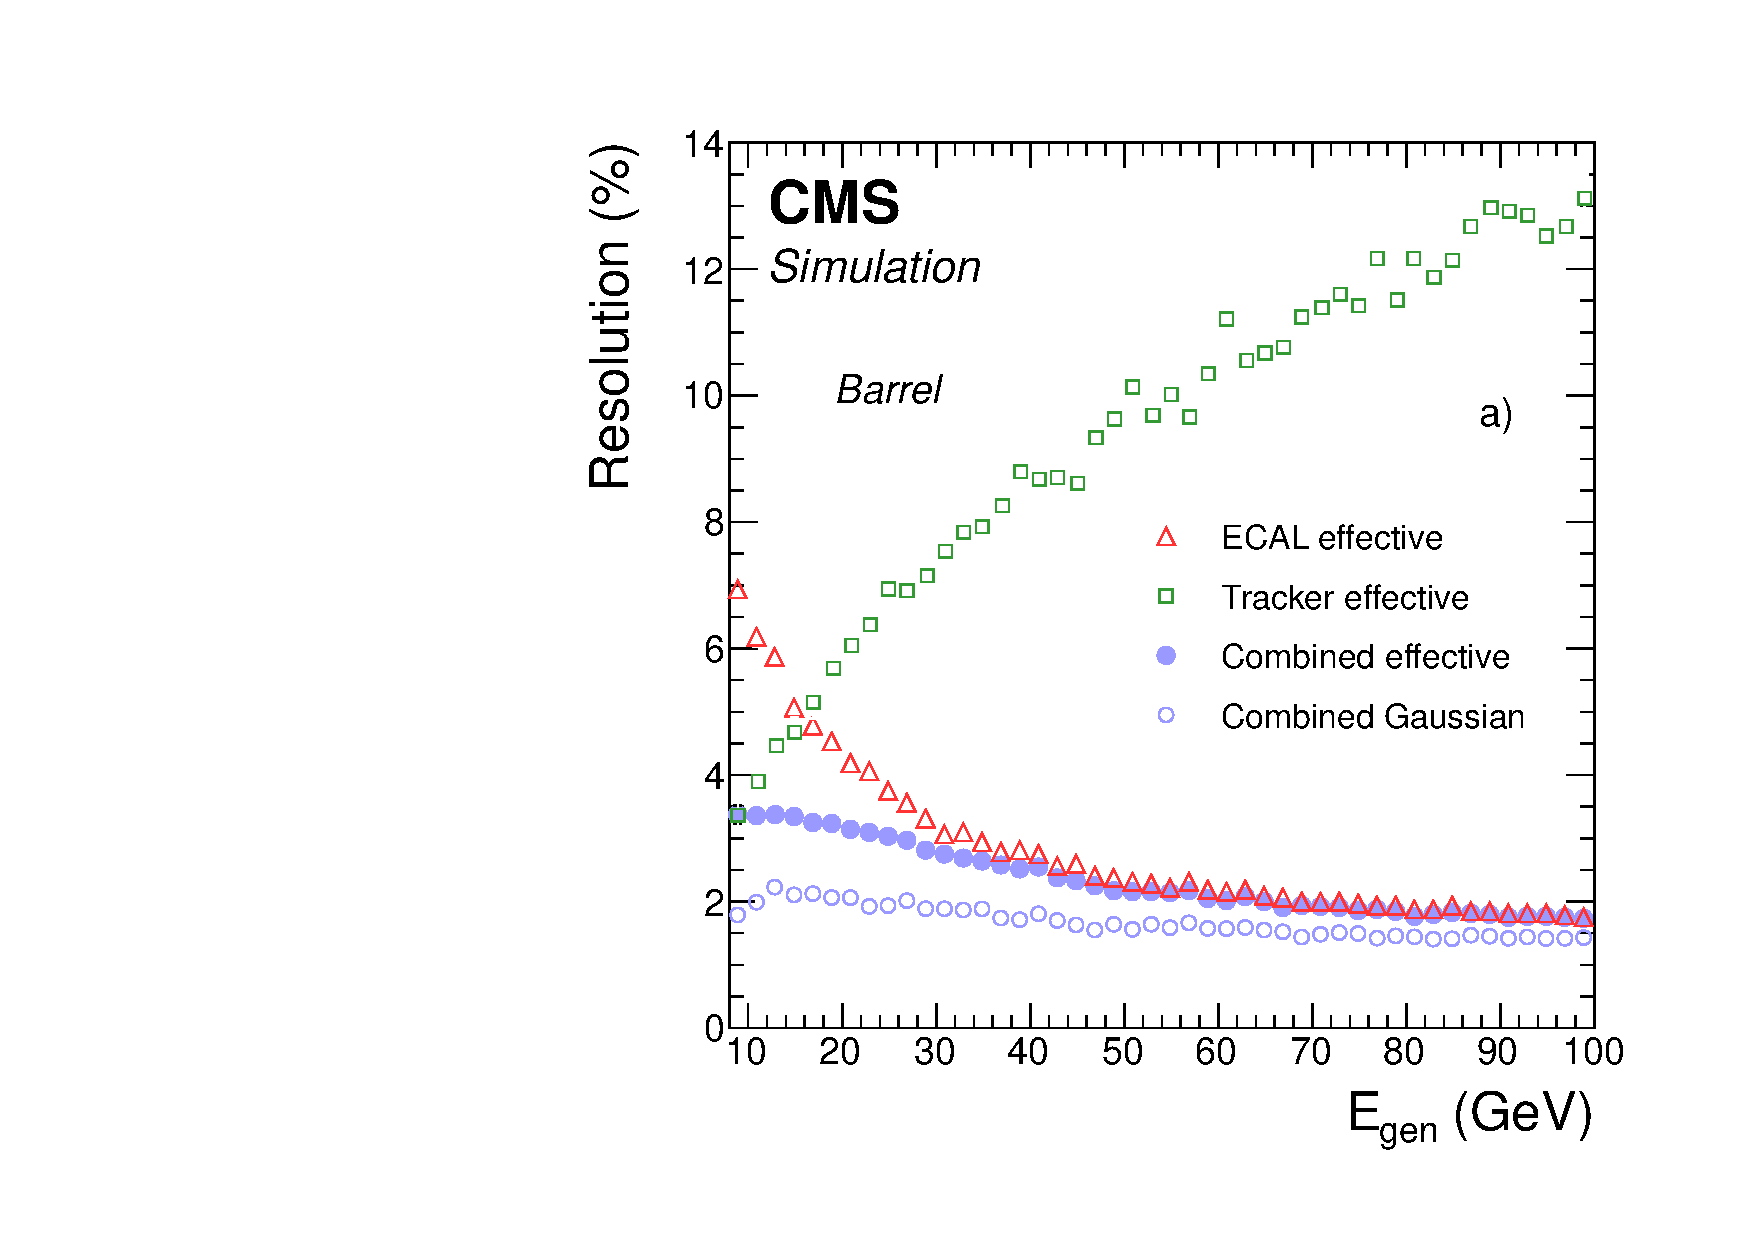
\includegraphics[width=0.45\textwidth]{\chsix/effRMSbarrel_withregression.pdf}
 \end{center}
 \caption{Expected resolution in \et for isolated electrons in the ECAL barrel as a function of the electron generated energy, obtained from the ECAL, the tracker and the combined estimates~\cite{Khachatryan:2015hwa}.}
 \label{fig:eleres}
\end{figure}

%%%%%%%%%%
\subsection{Electron trigger}\label{subsec:eletrigger}
%%%%%%%%%%

As explained in Section~\ref{subsec:CMStrigger}, the events of interest for physics analyses are selected by the trigger system in two steps, namely, the L1 and HLT.
%the trigger system consists of the layers: the Level 1 (L1) and the High Level Trigger (HLT).
At the L1, where the tracker information is not available, electrons and photons are indistinguishable and based on calorimeter trigger towers, consisting, in the barrel, of a $5\times5$ matrix of ECAL crystals and the corresponding HCAL tower, while a more complex definition of the tower is used in the endcaps. A L1 candidate is formed combining the highest-energy central trigger tower together with its next-highest adjacent tower.
At this stage, the trigger choice is based on the energy distribution among the central and neighbouring towers, on the amount of energy in the HCAL downstream the central tower, and on the \ET of the e/$\gamma$ candidate. 
%At this stage, the trigger choice is based only on the transverse energy of the calorimetric deposit, coarse shower shape requirements and the fraction of the total L1 seed energy belonging to the hadronic calorimeter, required to be smaller than 5\%.
%Two criteria on the shower shape are then applied: the ratio of the energy measured in the HCAL over the one in the ECAL is required to be less than 5\% and, in the barrel, 90\% of the ECAL energy must be contained in a 2 � 5 band of crystals in ? � ?. 
Events passing L1 are then filtered by the HLT. Here, the pixel tracker information is used to separate electrons from photons. The starting point of any electron HLT selection consists of building a supercluster and a trajectory as described in Section~\ref{subsec:elereco}. Many different triggers involving electrons are designed at the HLT level and various additional identification and isolation requirements on the electrons are made for each of them.
They consist of conditions on:

\begin{itemize}
\item transverse profile of the cluster of energy in the ECAL;
\item the amount of energy in the HCAL downstream the ECAL cluster;
\item the existence of a KF or GSF track matching the supercluster position;
\item quality of association between the track and the ECAL cluster;
\item activity in the ECAL, HCAL, or tracker around the candidate.
\end{itemize}

The conditions used and their severity depend on the number of electrons requested by the trigger and their transverse energy threshold, each trigger being designed to have a rate of accepting events of 50\unit{Hz} or less.
Practically, all the HLT steps and criteria involving only calorimeters information are done first, while the time consuming steps involving track reconstruction are only performed at the end for events passing the previous criteria.
The L1 and HLT triggers used to collect the data analyzed in this thesis are listed in Tables~\ref{tab:eletriggers8TeV} and~\ref{tab:eletriggers13TeV} for the 8 and 13\TeV data sets, respectively. The tables also detail the conditions imposed on several variables described in Section~\ref{subsec:eleid}.
Figure~\ref{fig:el_trig} shows the L1 trigger efficiencies for different \et thresholds as a function of the electron \et. The curves exhibit the typical turn on behaviour in correspondence of the imposed \et threshold.

\begin{table}[!htb]
\centering
\caption{The L1 and HLT single-electron triggers used to collect the 8\TeV data analyzed in this thesis together with the imposed requirements on the electron candidate.}
\resizebox{\textwidth}{!}{
\begin{tabular}{ l | c | c }
Trigger & Name & Selections\\
\hline
\hline
Level 1                     & L1\_SingleEG20                                                        & 1 e/$\gamma$ candidate \et $>$ 20 GeV\\
\hline
\multirow{6}{*}{HLT} & \multirow{6}{*}{HLT\_Ele80\_CaloIdVT\_GsfTrkIdT} & 1 GSF electron:\\
                                 &                                                                                   & \et $>$ 80\GeV\\
                                 &                                                                                   & $|\Delta\eta_{in}| < 0.008$\\
                                 &                                                                                   & $|\Delta\phi_{in}| < 0.07$ (barrel) or 0.05 (endcaps)\\
                                 &                                                                                   & $H/E < 0.05$\\
                                 &                                                                                   & $\sigma_{i\eta i\eta} < 0.011$ (barrel) or 0.031 (endcaps)\\
\end{tabular}}
\label{tab:eletriggers8TeV}
\end{table}

\begin{table}[!htb]
\centering
\caption{The L1 and HLT single-electron triggers used to collect the 13\TeV data analyzed in this thesis together with the imposed requirements on the electron candidate.}
\resizebox{\textwidth}{!}{
\begin{tabular}{ l | c | c }
Trigger & Name & Selections\\
\hline
\hline
\multirow{2}{*}{Level 1} & L1\_SingleEG35                                       & 1 e/$\gamma$ candidate \et $>$ 35 GeV\\
                                     & OR L1\_SingleEG40                                 & OR \et $>$ 40 GeV\\
\hline
\multirow{6}{*}{HLT}      &							             & 1 GSF electron:\\
                                     &   							     & \et $>$ 105\GeV OR $>$ 115\GeV\\
                                     & 	HLT\_Ele105\_CaloIdVT\_GsfTrkIdT	     & $|\Delta\eta_{in}| < 0.008$\\
                                     & 	OR HLT\_Ele115\_CaloIdVT\_GsfTrkIdT & $|\Delta\phi_{in}| < 0.07$ (barrel) or 0.05 (endcaps)\\
                                     & 							              & $H/E < 0.05$\\
                                     & 							              & $\sigma_{i\eta i\eta} < 0.011$ (barrel) or 0.031 (endcaps)\\
\end{tabular}}
\label{tab:eletriggers13TeV}
\end{table}

\begin{figure}[!htb]
\centering
\subfigure[]{\label{fig:el_trig_a}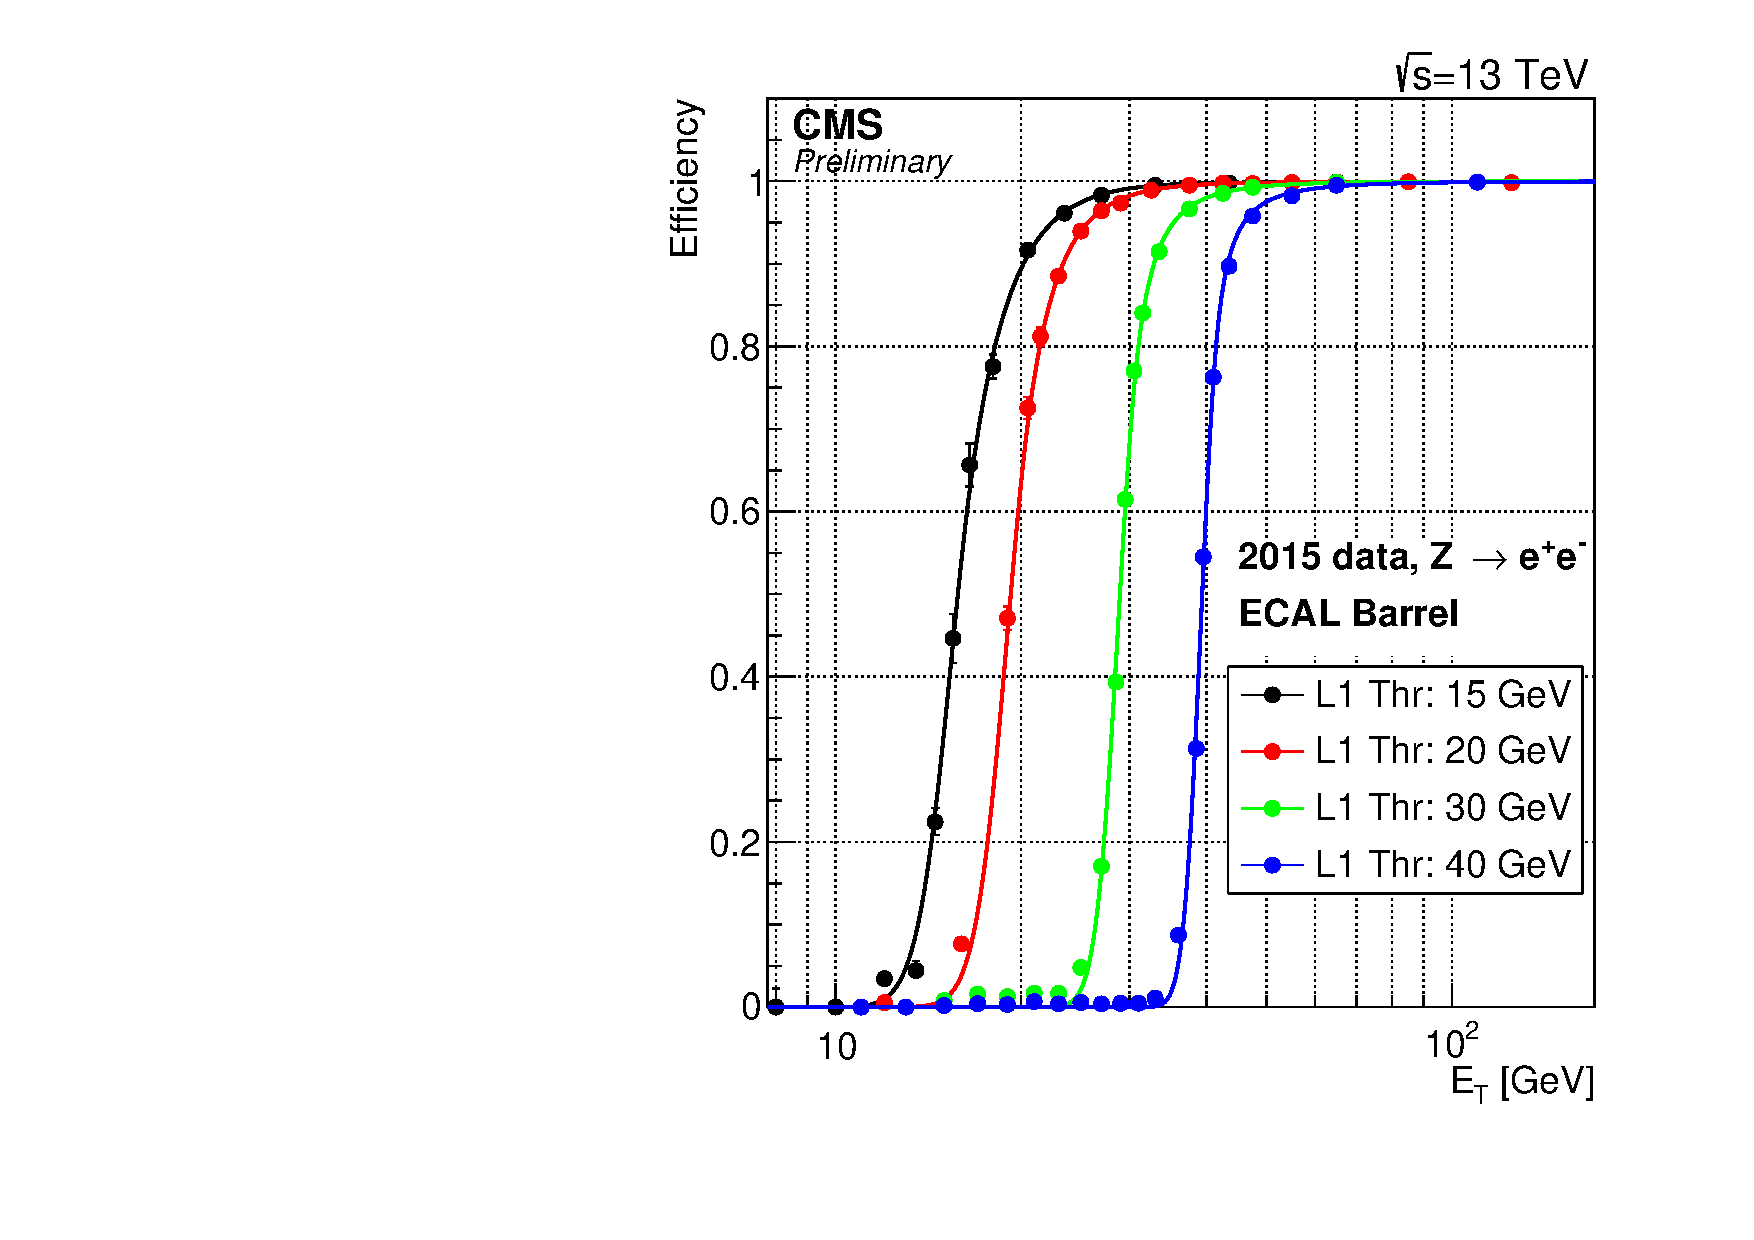
\includegraphics[width=0.45\textwidth]{\chsix/plot_iEG_2015.pdf}}
\subfigure[]{\label{fig:el_trig_b}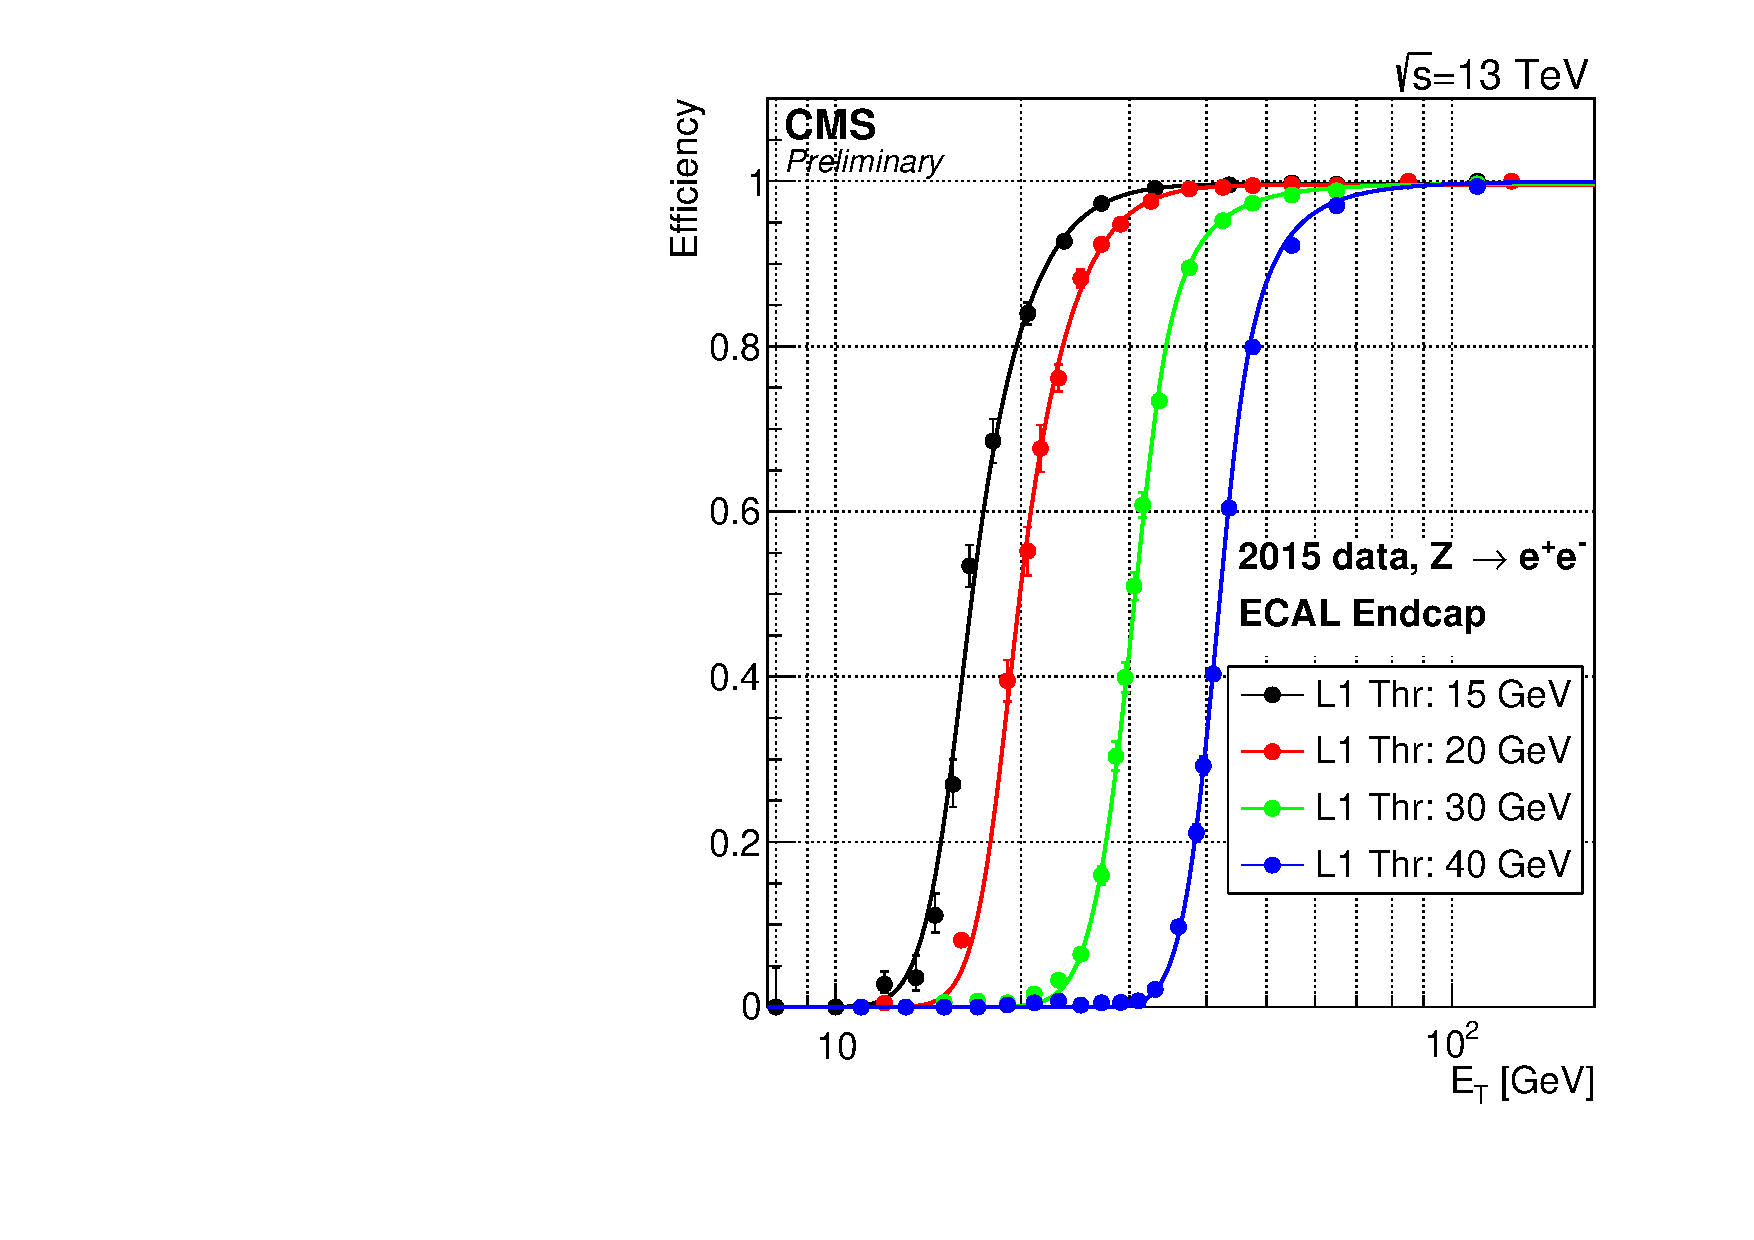
\includegraphics[width=0.45\textwidth]{\chsix/plot_EE_iEG_2015.pdf}}
\caption{L1 electron triggering efficiency in ECAL barrel (a) and endcaps (b) as a function of the offline reconstructed electron \et. The efficiency is shown for the 15, 20, 30, 40\GeV EG trigger thresholds~\cite{ECALPublicResults}.}
\label{fig:el_trig}
\end{figure}

Both the L1 and HLT triggers require one electron (or $\gamma$) candidate.  
The \et thresholds imposed for the data collected in pp collisions at 13\TeV are higher compared to the one used in Run~1, in order to keep low trigger rates given the higher production rates of low-energy multijet background expected in Run~2. The chosen HLT triggers require a reconstructed GSF track whose association to the ECAL cluster has to pass tight quality criteria ($|\Delta\eta_{in}|$ and $|\Delta\phi_{in}|$).
Requirements are also applied at this level on the transverse profile of the cluster of energy in the ECAL ($\sigma_{i\eta i\eta}$) and on the amount of energy in the HCAL downstream the ECAL ($H/E$). There are no requirements imposed on the electron candidate isolation. 
In general, this results in high fake rates of jets misreconstructed as electrons from multijet background, and, as a consequence, in high trigger rates which would require a prescale. However, the high \et threshold allows for an unprescaled trigger, as jets from multijet background are characterized by low momentum. In addition, the kinematic region of the analyses presented in this thesis is located at very high lepton \pt and the signal efficiency is mainly affected at very low resonance masses ($< 1\TeV$) with a loss in efficiency of 20--25\%.\\
%The offline reconstructed \pt of the electrons must be greater than 90 (120) \GeV for the 8 (13) TeV analysis, where the trigger reaches the plateau. In fact, this choice is made to simplify the analysis avoiding the need for modelling the trigger turn-on curve and, as a consequence, reducing the associated systematic uncertainties.

The efficiency for an electron passing the high-\et selections described in Sec.~\ref{subsec:eleid} to fire the HLT triggers of Tables~\ref{tab:eletriggers8TeV} and \ref{tab:eletriggers13TeV} have been measured in data with T\&P method and are found to be 98-99\% for electrons with \et in the trigger plateau, with data-to-simulation scale factors close to unity.
%The efficiency for a HEEP electron to pass the HLT_Ele105 are 0.984 (barell) 0.998 (endcap) in the plateau. For HLT115 are 0.971/0.966. (W' analysis AN-2015/226)
%from W'->l+MET 8 TeV: The trigger efficiency for single electrons has been determined with ?tag-and-probe? methods [65] to be 99.1 (97.6)% for the barrel (endcap) ECAL, with a data-to-simulation scale factor of nearly one. (https://arxiv.org/pdf/1408.2745v2.pdf)

%%%%%%%%%%
\subsection{Electron identification}\label{subsec:eleid}
%%%%%%%%%%

All the physics analyses in CMS involving one or two electrons in the final state start with the general electron reconstruction algorithm presented in Section~\ref{subsec:elereco}.
%The electron reconstruction presented in Section~\ref{subsec:elereco} is the starting point of any electron selection in CMS and it is used by any physics analysis involving one or several electrons in the final state.
A high efficiency in any kinematical conditions is therefore needed and, as a consequence, the probability for other particles to be reconstructed as electrons is sizeable.
For instance, a charged pion can mimic the signature of an electron if it interacts early and leaves most of its energy in the ECAL. Moreover electrons can emerge in a jet through the weakly decay of a hadron containing a c or b quark. Finally, in addition to jets, photons can also lead to GSF electron candidates. This happens if the photon converts into a dielectron pair in one of the first layers of the tracker detector. If one of the electron takes most of the photon momentum, a GSF electron candidate is likely to be reconstructed.
%In fact, the GSF electron candidates reconstructed in the data are mainly other physics objects misreconstructed as electrons, or ``fakes''. These fakes are of several kinds: a charged pion can for instance mimic the signature of an electron if it interacts early and leaves most of its energy in the ECAL. Moreover electrons can emerge in a jet through the weakly decay of a hadron containing a c or b quark. Finally, in addition to jets, photons can also lead to GSF electron candidates. This happens if the photon converts into a dielectron pair in one of the first layers of the tracker detector. If one of the electron takes most of the photon momentum, a GSF electron candidate is likely to be reconstructed.
An analysis dependent selection, which takes into account the specific kinematics and background level, has therefore to be applied on top of the electron reconstruction. This thesis focuses on the search for massive resonances decaying to pairs of SM bosons where one of the bosons is a W decaying leptonically, with a highly energetic electron or muon in the final state. A high and stable selection efficiency for \et above 100\GeV is therefore an important requirement.
%Most of the searches for new physics involving high energy electrons share the same features:
%-The cross sections probed are tiny (sometimes below 1 fb).
%-The background due to jets or other particles wrongly reconstructed as GSF electron candidates is moderate.
%-The electron energy range under study is large (from ET = 100 GeV to ? 1 TeV).
%-The usual control region to check the performance of an electron selection in the data is the Z peak, where a large statistics is available for electrons with ET ? 35 GeV.
%-For higher ET values, the control regions (events with boosted on-shell Z or high mass tail of the Drell-Yan process) suffer from low statistics.
%A high and stable selection efficiency for ET above 100GeV is therefore the main requirement. The selection must also reasonably work for lower values, down to 35 GeV. Finally, given the fact that the validation of the selection at high ET in data is difficult, a simple and understandable selection is preferred.
Since this is a common feature of many searches for new physics, a specific cut based selection has been developed in CMS~\cite{Khachatryan:2014fba}, consisting of requirements on several variables that exploit the characteristics of high-\et electrons. Only GSF electron candidates with $\et > 35\GeV$ and well reconstructed in the tracker and ECAL sensitive regions are selected. Candidates in the ECAL transition region ($1.442 < |\eta_\mathrm{SC}| < 1.56$) and beyond the $\eta$ coverage ($|\eta_\mathrm{SC}|  > 2.5$) of the tracker are therefore discarded. A different selection is applied for candidates reconstructed in the ECAL barrel ($|\eta_\mathrm{SC}| < 1.442$) and endcaps ($1.56 < |\eta_\mathrm{SC}|  < 2.5$). For Run~2 the values of $\eta_\mathrm{SC}$ have been slightly adjusted to match the acceptance of the detector more accurately. The selections are summarized in Tables~\ref{tab:heep8TeV} and \ref{tab:heep13TeV}, for the 8 and 13\TeV data analysis, respectively, and discussed in the following.

%https://twiki.cern.ch/twiki/bin/viewauth/CMS/HEEPElectronID
\begin{table}[!htb]
\centering
\caption{List of the variables used in the high-\et electron selections for the 8\TeV data analysis, together with the corresponding requirements for electrons reconstructed in the ECAL barrel and endcaps.}
\resizebox{\textwidth}{!}{
\begin{tabular}{ l | c | c }
Variable & ECAL barrel & ECAL endcaps\\
\hline
\hline
ECAL-driven & yes & yes\\ 
\et & $> 35\GeV$ & $> 35\GeV$\\
$|\eta_{\mathrm SC}|$ & $< 1.442$ & 1.56--2.5\\
$|\Delta\eta_{in}|$ & $< 0.005$ & $< 0.007$\\
$|\Delta\phi_{in}|$ & $< 0.06$ & $< 0.06$\\
Relative track isolation & 5\% & 5\% \\
\multirow{2}{*}{Calorimeter isolation} & \multirow{2}{*}{$< 2 + 0.03\et +0.28\rho$} & $< 2.5 + 0.28\rho$ if $\et < 50$\\
 & & $< 2.5 + 0.03(\et-50) + 0.28\rho$ if $\et \geq 50$\\  
\multirow{2}{*}{Transverse shower shape} & $E_{2\times5}/E_{5\times5} > 0.94$ & \multirow{2}{*}{$\sigma_{i\eta i\eta} < 0.03$} \\
  & OR $E_{1\times5}/E_{5\times5} > 0.83$ & \\
%$\sigma_{i\eta i\eta}$ & - & $< 0.03$\\
$H/E$ & $< 0.05$ & $< 0.05$\\
$|d_{xy}|$ & $< 0.02$ & $< 0.05$\\
Inner layer lost hits & $\leq 1$ & $\leq 1$\\
\end{tabular}}
\label{tab:heep8TeV}
\end{table}

\begin{table}[!htb]
\centering
\caption{List of the variables used in the high-\et selections for the 13\TeV data analysis, together with the corresponding requirements for electrons reconstructed in the ECAL barrel and endcaps.}
\resizebox{\textwidth}{!}{
\begin{tabular}{ l | c | c }
Variable & ECAL barrel & ECAL endcaps\\
\hline
\hline
ECAL-driven & yes & yes\\ 
\et & $> 35\GeV$ & $> 35\GeV$\\
$|\eta_{\mathrm SC}|$ & $< 1.4442$ & 1.566--2.5\\
$|\Delta\eta_{in}|$ & $< 0.004$ & $< 0.006$\\
$|\Delta\phi_{in}|$ & $< 0.06$ & $< 0.06$\\
Relative track isolation & 5\% & 5\% \\
\multirow{2}{*}{Calorimeter isolation} & \multirow{2}{*}{$< 2 + 0.03\et +0.28\rho$} & $< 2.5 + 0.28\rho$ if $\et < 50$\\
 & & $< 2.5 + 0.03(\et-50) + 0.28\rho$ if $\et \geq 50$\\  
\multirow{2}{*}{Transverse shower shape} & $E_{2\times5}/E_{5\times5} > 0.94$ & \multirow{2}{*}{$\sigma_{i\eta i\eta} < 0.03$} \\
  & OR $E_{1\times5}/E_{5\times5} > 0.83$ & \\
%$\sigma_{i\eta i\eta}$ & - & $< 0.03$\\
$H/E$ & $< 1/E + 0.05$ & $< 5/E + 0.05$\\
$|d_{xy}|$ & $< 0.02$ & $< 0.05$\\
Inner layer lost hits & $\leq 1$ & $\leq 1$\\
\end{tabular}}
\label{tab:heep13TeV}
\end{table}
%https://twiki.cern.ch/twiki/bin/view/CMS/HEEPElectronIdentificationRun2#Selection_Cuts_HEEP_V6_0_Recomme

As a starting point, electrons are selected if the reconstruction was seeded in the ECAL (Section~\ref{subsec:elereco}). In fact, while useful for low-energy and non-isolated electrons, the PF algorithm is less suitable for high-energy electrons.

%deltaEta/deltaPhi in
The difference in $\eta$, $\Delta\eta_{in}$, and in $\phi$, $\Delta\phi_{in}$, between the track position as measured in the inner layers, extrapolated to the interaction vertex and to the calorimeter, and the position of the supercluster, are required to be $< 0.005$ and $< 0.06$, respectively. In fact, for jets, the position of the center of the ECAL deposit can be far from the track position, as all of the constituents can leave an energy deposit in the ECAL. The $\Delta\phi_{in}$ distribution is however much broader than $\Delta\eta_{in}$, because of the wider spread of the energy in $\phi$ due to photons from bremsstrahlung, resulting in a looser requirement. The distributions of $\Delta\phi_{in}$ and $\Delta\eta_{in}$ become narrower with increasing \et, and therefore a higher discrimination power can be achieved with a tighter requirement at high \et compared to the usual selections for low or intermediate energetic electrons. The reason of this behaviour comes from the fact that bremsstrahlung photons are more collinear to the electron at higher \et. The definition of $\Delta\eta_{in}$ has been changed for Run~2 to use instead the $\eta$ of the seed cluster of the supercluster which is found to provide a more accurate indication of the $\eta$ of the original electron before bremsstrahlung. 

%trackIso
To suppress the misidentification of jets as electrons, the sum of the \pt of all other tracks in a cone of $\Delta R < 0.3$ around the track of the electron candidate is required to be less than 5\GeV, imposing an isolation condition on the electron candidate track. To be used in the calculation of the isolation of the candidate track, the tracks have to be within 0.2\cm, in the $z$ direction, of the primary vertex with which the electron candidate is associated. This requirement reduces the impact of pileup and it does not show a dependency with the electron \et for values above 100\GeV.
%For electrons with transverse energies above 100\GeV, a negligible change in the selection efficiency is observed as the number of pileup events increases from 0 to 40.
For electrons with \et much lower than 100\GeV, the efficiency decreases up to 10\% depending on the region of the detector in which the electrons are detected. 

%ECAL+HCAL1 iso
A calorimeter-based isolation is applied and defined as the sum of:

\begin{itemize}
\item ECAL isolation: sum of the \et of the energy deposits in the ECAL calorimeter in a cone of $\Delta R < 0.3$ around the track of the electron candidate excluding those associated with the candidate;
\item HCAL1 isolation: sum of the \et of the energy deposits in the first layer of the HCAL calorimeter in a cone of $\Delta R < 0.3$ around the track of the electron candidate excluding those associated with the candidate.
\end{itemize}

The isolation variable so defined, is required to be less than 3\% (plus a small $\eta$-dependent offset) of the candidate \et.
%Within this same cone, the sum of the \et of the energy deposits in the calorimeter that are not associated with the candidate is required to be less than 3\% (plus a small $\eta$-dependent offset) of the candidate \et.
This sum, which allows a selection on the isolation of the electron candidate, is corrected for the average energy density in the event, $\rho$, to minimize the dependence of the efficiency of this selection criterion on pileup. 
This requirement differs from the selection usually applied for electrons of low or intermediate \et. For these cases, a PF-based isolation is generally used, which merges the information of the tracker, the ECAL and the HCAL allowing to measure the contribution to the isolation from charged hadrons, neutral hadrons and photons separately. One of the main advantage of the PF-based isolation is that the energy deposit in the calorimeters associated to a charged hadron produced in another interaction, characterized by a different primary vertex, can be removed from the isolation sum. For very high energy ($ > 1\TeV$) electrons, however, the PF algorithm might fail to recognize an electron from a GSF electron candidate and assigns all its energy deposit to the photon isolation. 
Furthermore, the PF isolation is generally required to be below a fixed fraction of the electron \et independently on its value.
However, for high \et values the background rejection can be improved while keeping an acceptable efficiency by following the \et dependence of the ECAL+HCAL1 isolation variable.
In fact, this isolation tends to increase for high-\et electrons due to the extension of the shower.
%To better follow the ET evolution and hence improve the background rejection while keeping an acceptable efficiency at moderate ET the HEEP cut value is of the form Iso < A + B � ET . 
%This requirement is suitable for electrons with \et in the low or intermediate range ($\et < 50--100\GeV$) but it results in a very loose selection for electrons with much higher \et (150\GeV for $\et = 1\TeV$).
%This is perfectly acceptable at moderate ET (ET < 50-100 GeV) but this would mean a cut value of 150 GeV for an electron with ET = 1 TeV which is far above the typical values for real electrons.

%H/E + profile
Further suppression of the misidentification of jets as electrons is
achieved by requiring that the ratio $H/E$ of the energy in the HCAL towers in a cone of $\Delta R < 0.15$ centered on the electron candidate position, to the electromagnetic energy of the electron candidate supercluster is required to be less than 5\%. This requirement is tighter compared with the threshold applied for low- or medium-energy electrons, where it becomes quite inefficient for a high number of pileup interactions.
%where the contribution from pileup. Therefore, a weaker selection is applied to avoid large signal inefficiencies.
For Run~2, the selection on this variable has been increased.
Additionally, the transverse profile of the energy deposition in the ECAL is required to be consistent with that expected for an electron, being defined by the following variables:

\begin{itemize}
\item $E_{1\times5}/E_{5\times5}$: ratio of the energy contained in the 1$\times$5 matrix in $\eta\times\phi$ in the barrel ($x\times y$ in the endcaps) centered on the seed crystal of the supercluster over the energy of the $5\times5$ matrix centered on the seed crystal;
\item $E_{2\times5}/E_{5\times5}$: ratio of the energy contained in the most energetic 2$\times$5 matrix in $\eta\times\phi$ in the barrel ($x\times y$ in the endcaps) centered on the seed crystal of the supercluster over the energy of the $5\times5$ matrix centered on the seed crystal;
\item $\sigma_{i\eta i\eta}$ : measure of the spread in $\eta$ in units of crystals of the electrons energy in the $5\times5$ block centered on the seed crystal.
\end{itemize}

In the barrel, the best performance are obtained applying a selection on both $E_{1\times5}/E_{5\times5}$ and $E_{2\times5}/E_{5\times5}$.
The two variables are indeed complementary: while $E_{1\times5}/E_{5\times5}$ is well designed for electrons hitting the center of a crystal, $E_{2\times5}/E_{5\times5}$ allows to recover electrons that hit the crystal close to its edge. Combining the two variables instead of using just one of them allows to set a  tight requirement on both and thus well reject background while keeping a high efficiency on simulated electrons. 
The distributions of these variables are much broader for electrons in the endcaps and a higher discrimination power is obtained applying a selection on the variable $\sigma_{i\eta i\eta}$.
%This is because the x ? y geometry does not follow the ? ? ? direction. As a consequence, part of the energy is sometimes missing in both E1�5/E5�5 and E2�5/E5�5 and their discrimination power is reduced and becomes worse than ?i?i?.
%H/E
%The cut value (0.05) is sensibly lower than the one usually used at moderate ET (0.12 in the barrel and 0.10 in the endcaps). At moderate ET this cut is indeed quite inefficient for a high number of pile-up interactions in the event ... why?

%missing hits + dxy
Two additional requirements are applied to reject photons that convert into a electron-positron pair in the tracker.
First, the track associated with the cluster is required to have no more than one hit missing in the pixel layers.
%It is mainly designed to reject photons that convert into a pair in the tracker as can be seen from figure 4.14. It can happen that only one of the electron tracks is reconstructed.
IN fact, the signature arising from photon conversion process is very similar to the one from real electrons, and the gain in discrimination using shower shape variables is limited. However, one of the main differences is the absence of hits in the first layers of the tracker, before the conversion happens.
Furthermore, the transverse impact parameter $d_{xy}$, defined as the closest distance, in the transverse plane, between the primary vertex and the track of the electron candidate, is required to be $< 0.02\cm$ (barrel) or 
$0.05\cm$ (endcaps). The distribution of the transverse impact parameter is usually wider in the endcaps due to the poorer resolution of the track position in that region.\\

The efficiency of the high-\et electron selection measured with the T\&P method in pp collisions at $\sqrt{s} = 8\TeV$ and in simulation as a function of the electron \pt is shown in Fig.~\ref{fig:el_heep}, for electrons reconstructed in the ECAL barrel and endcaps. Similar results are obtained using 13\TeV data. The efficiencies and data-to-simulation scale factors are summarized in Tables~\ref{tab:heepsf8TeV} and~\ref{tab:heepsf13TeV}, as measured in 8 and 13\TeV data and simulation, respectively. The scale factors are close to unity, indicating a good agreement between data and simulation. They are used in the analysis presented in this thesis to correct the normalization of simulations.

\begin{figure}[!htb]
\centering
\subfigure[]{\label{fig:el_heep_a}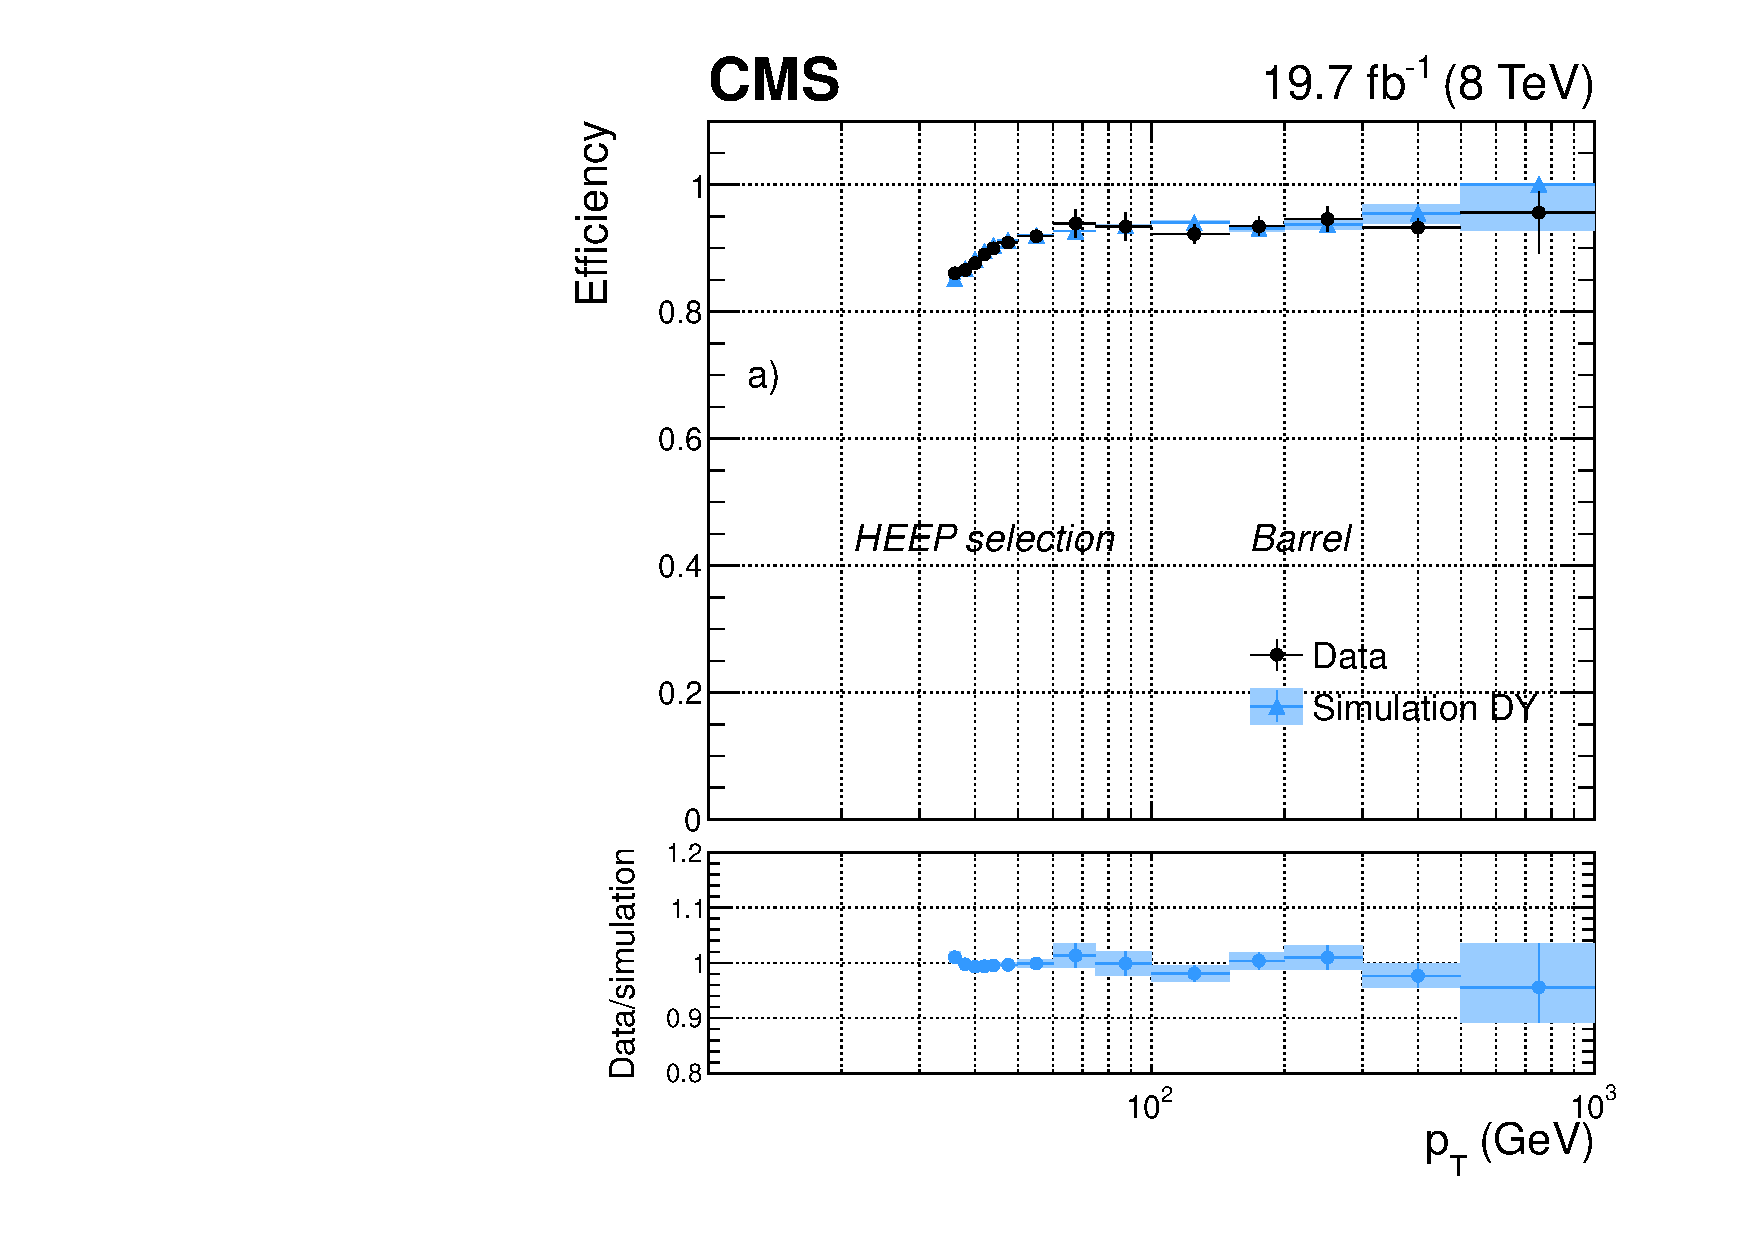
\includegraphics[width=0.45\textwidth]{\chsix/HEEPSF_barrel.pdf}}
\subfigure[]{\label{fig:el_heep_b}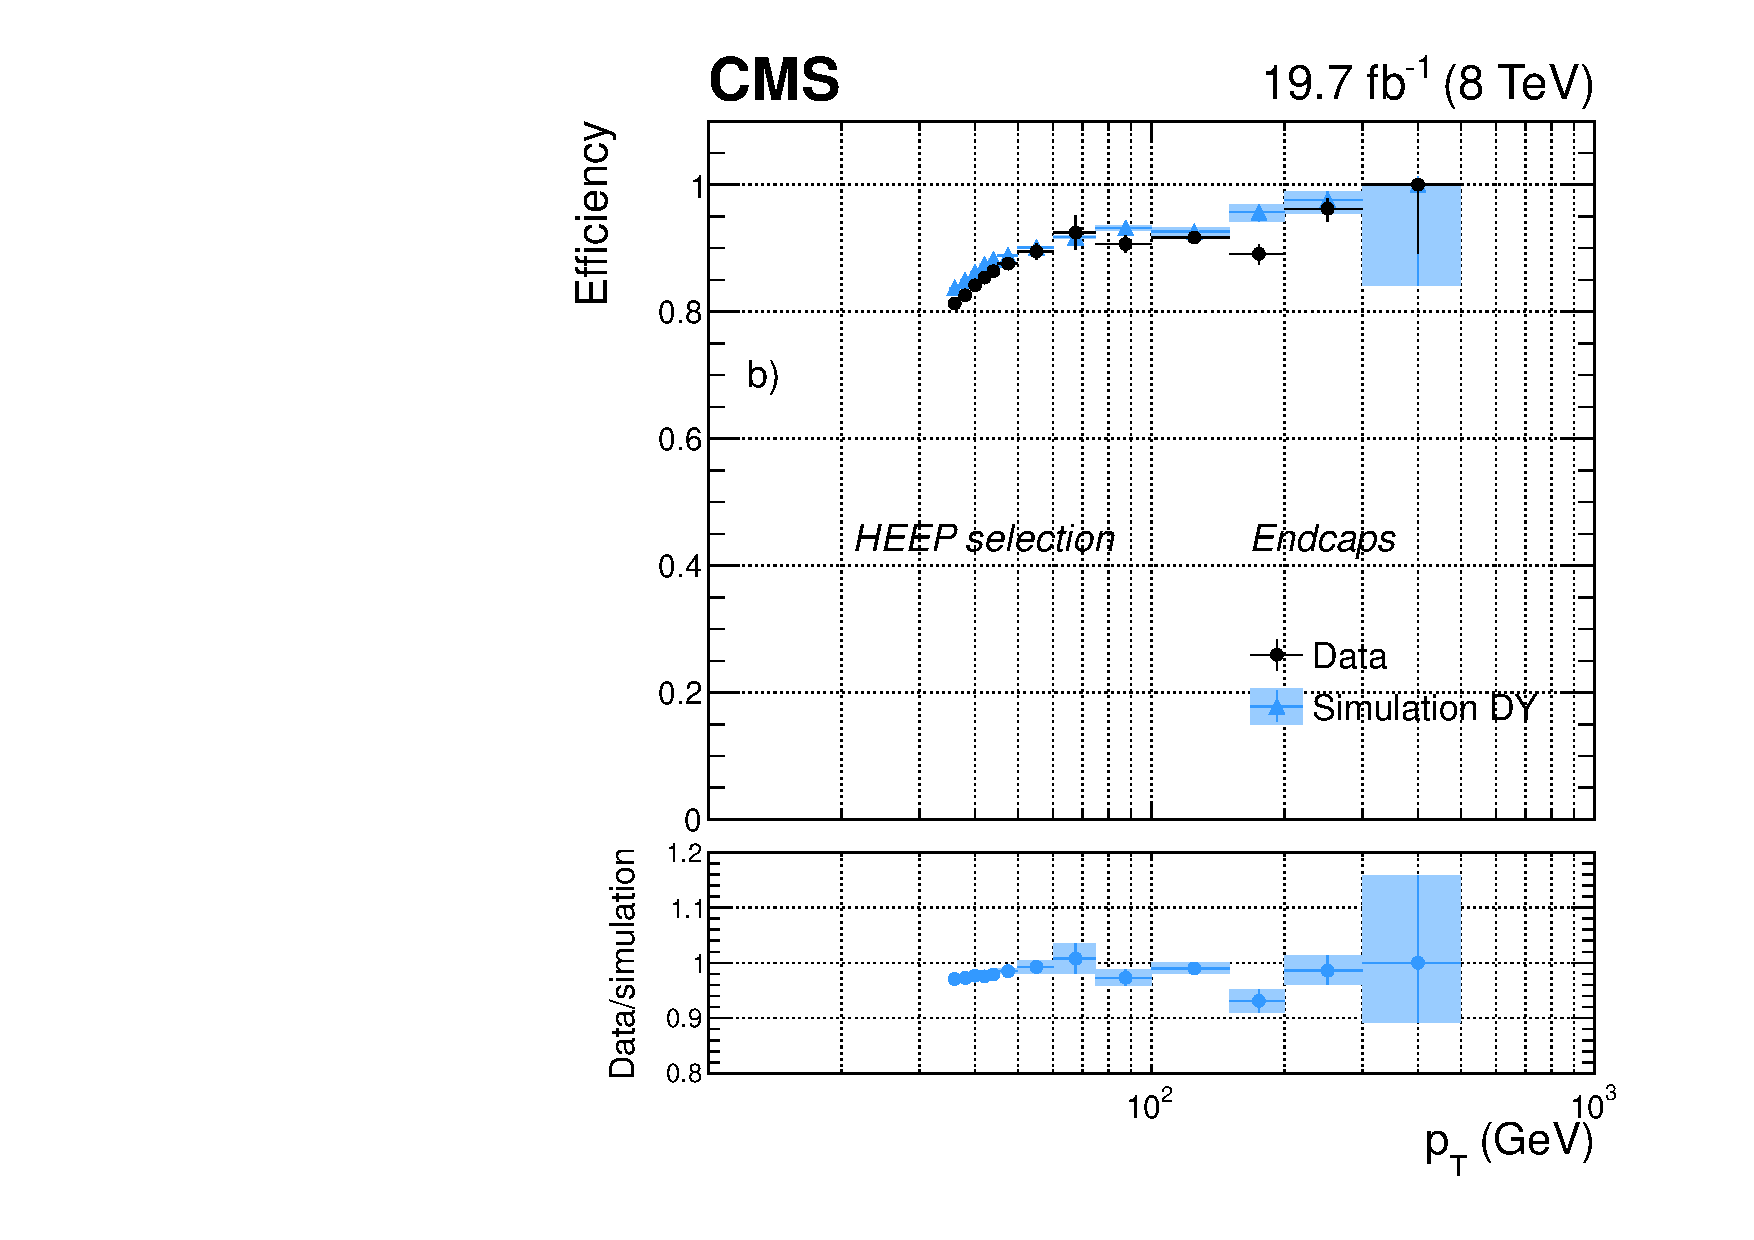
\includegraphics[width=0.45\textwidth]{\chsix/HEEPSF_endcaps_corr_noeffgt1.pdf}}
\caption{Efficiency of the high-\et electron selection as a function of electron \pt for dielectron events in pp collisions at $\sqrt{s} = 8\TeV$ (dots) and in DY simulation (triangles) for electrons reconstructed in the ECAL barrel (a), and endcaps (b)~\cite{Khachatryan:2015hwa}.}
\label{fig:el_heep}
\end{figure}

\begin{table}[!htb]
\centering
\caption{Efficiencies and data-to-simulation scale factors for the high-\et electron selection, as measured in pp collisions at $\sqrt{s} = 8\TeV$ for electrons with $\et > 90\GeV$. The quoted uncertainties are statistical.}
\begin{tabular}{ c | c | c}
 & ECAL barrel & ECAL endcaps\\
\hline
\hline
Efficiency simulation & 90.2\% $\pm$ 0.2\% & 92.2\% $\pm$ 0.5\%\\
Efficiency data & 88.7\% $\pm$ 0.2\% & 90.7\% $\pm$ 0.6\%\\
Data/simulation scale factor & 0.983 $\pm$ 0.004 & 0.984 $\pm$ 0.010 \\
\hline 
\end{tabular}
\label{tab:heepsf8TeV}
\end{table}
%https://twiki.cern.ch/twiki/bin/viewauth/CMS/HEEPEfficiencies#Efficiencies_and_scale_factors_f

\begin{table}[!htb]
\centering
\caption{Efficiencies and data-to-simulation scale factors for the high-\et electron selection as measured in pp collisions at $\sqrt{s} = 13\TeV$ for electrons with $\et > 120\GeV$. The quoted uncertainties are statistical.}
\begin{tabular}{ c | c | c}
 & ECAL barrel & ECAL endcaps\\
\hline
\hline
Efficiency simulation & 91.4\% $\pm$ 0.10\% & 84.4\% $\pm$ 0.3\%\\
Efficiency data & 91.6\% $\pm$ 0.04\% & 82.3\% $\pm$ 0.1\%\\
Data/simulation scale factor & 1.002 $\pm$ 0.001 & 0.975 $\pm$ 0.004\\
\hline 
\end{tabular}
\label{tab:heepsf13TeV}
\end{table}
%from Z'->ll AN-2015/222

 
%%%%%%%%%%
%\section{Muons}\label{sec:muons}
 %%%%%%%%%%%%%%%%%%%%%%%%%%%%%%%%%%%%%%%%%%%%%%%%%%%%%%%%%%%%%%%
\section{Muons}\label{sec:muons}
%%%%%%%%%%%%%%%%%%%%%%%%%%%%%%%%%%%%%%%%%%%%%%%%%%%%%%%%%%%%%%%

%%%%%%%%
\subsection{Muon reconstruction}
%%%%%%%%

The CMS detector is specifically designed for the optimization of muon detection, as its name clearly states. 
%Indeed the detection and high precision measurement of muons play key roles in many physics processes of interest such as the ones described in this thesis.
%The detection and high precision measurement of muons is very important for CMS. Many processes of interest involve muons in their final states, like the Higgs decay channel H$\rightarrow$ZZ$\rightarrow$4$\mu$ . In fact, CMS is specifically designed for the optimization of muon detection, as its name clearly states.
In general, muons will not be absorbed by the calorimeters, as is what happens with electrons, so a specific muon detection system (Section~\ref{subsec:muonchambers}) is needed in order to identify them.\\
%and improve the resolution of their momenta as measured by the tracking system.\\

In the standard CMS reconstruction~\cite{Chatrchyan:2012xi}, tracks are first reconstructed independently in the inner tracker (tracker track) and in the muon system (standalone-muon track).
%Based on these objects, two reconstruction approaches are used:
A standalone-muon track is reconstructed from pre-built track segments (i.e. a set of aligned DT or CSC hits) in the muon chambers. The state vector associated to the segments found in the innermost chambers is used to seed the muon trajectory, from inside out, using the KF technique: the predicted state vector at the next measurement surface is compared with existing hits and updated accordingly. A suitable $\chi^2$ cut is applied to reject bad hits and the procedure is iterated until the outermost surface of the muon system is reached. Finally, the track is extrapolated to the nominal interaction point and a vertex-constrained fit is performed. The magnetic field, the multiple scattering inside the steel yoke, and the energy loses are taken into account.

Based on reconstructed standalone-muon and tracker tracks, two reconstruction approaches are then used:

\begin{itemize}
\item {\bf global-muon reconstruction (outside-in)}: each standalone-muon track is extrapolated to the tracker and a search is performed in a cone around it to match a tracker track; a global-muon track is fit combining hits from the tracker track and standalone-muon track, using the KF technique;
\item {\bf tracker-muon reconstruction (inside-out)}: all tracker tracks with $\pt > 0.5\GeV$ are considered as possible muon candidates and are extrapolated to the muon system while searching for a match with at least one muon segment.
\end{itemize}

Tracker-muon reconstruction is more efficient than the global-muon reconstruction at low momenta, $\pt \leq$ 5\GeV, because it requires only a single muon segment in the muon system, whereas global-muon reconstruction is designed to have high efficiency for muons penetrating through more than one muon station, and typically requires segments in at least two muon stations. However, given the high efficiency of both the tracker track and muon segments reconstruction, about 99\% of muons produced within the geometrical acceptance of the muon system and having sufficiently high momentum ($\pt \geq$ 5\GeV) are reconstructed by both methods. As shown in Fig.~\ref{fig:mu_ptrel} the additional information provided by the muon system is precious for the momentum reconstruction of high-energy muons ($\pt \geq$ 200\GeV), for which the tracker-only momentum measurement is degraded. 
In fact, as a particle's momentum increases and the curvature of its corresponding track decreases, the momentum resolution in the tracker becomes limited by position measurement resolution. One can then benefit from the large lever arm and 3.8\unit{T} magnetic field in the region between the tracker and the muon system by including hits in the muon chambers. For lower momenta, instead, the resolution of the tracking system is dominating.
%At large transverse momenta, pT $\geq$ 200\GeV/c, the global-muon fit can improve the momentum resolution compared to the tracker-only fit.
%A tracker muon is less restrictive in the muon system reconstruction (only requires a muon segment) so it will be slightly more efficient for low-pT muons, which might not cross enough muon stations as to reconstruct a standalone track. 

\begin{figure}[!htb]
\centering
\subfigure[]{\hspace{-0.7cm}\label{fig:mu_ptrel_a}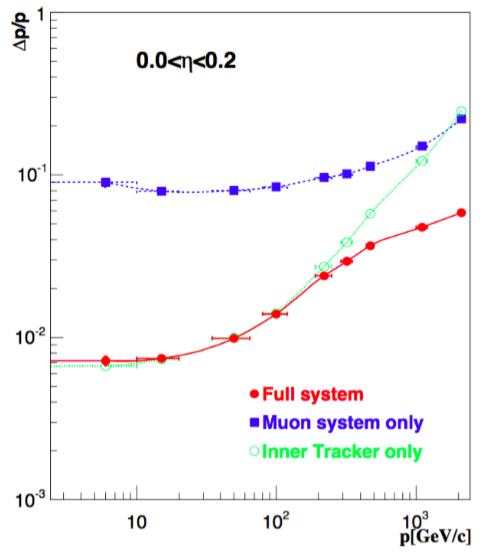
\includegraphics[width=0.38\textwidth]{\chsix/muon-pt-resolution-etabin0.png}}\quad\quad\quad
\subfigure[]{\hspace{-0.7cm}\label{fig:mu_ptrel_b}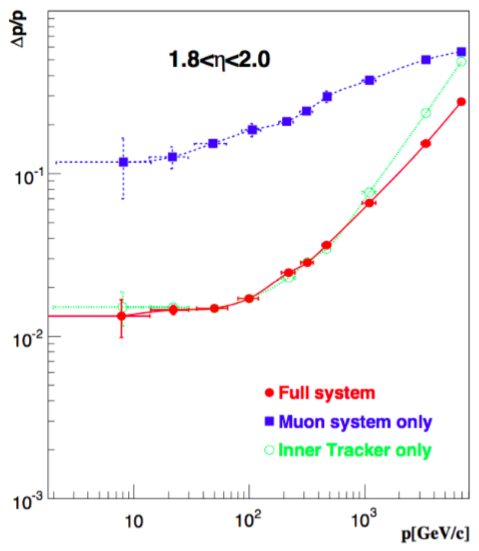
\includegraphics[width=0.38\textwidth]{\chsix/muon-pt-resolution-etabin1.png}}
\caption{Relative resolution of the muon momentum measurement for the reconstruction with the inner tracker only, the muon system only and for the combination of the inner tracker and the muon system, for simulated muons emitted in the central (a) and forward (b) regions~\cite{Bayatian:922757}.}
\label{fig:mu_ptrel}
\end{figure}

Figure~\ref{fig:mu_reco_eff} shows the muon tracking efficiency as a function of the $\eta$ of the probe muon and the number of primary vertices for 13\TeV data and simulation, evaluated using the T\&P method described in Section~\ref{subsec:elereco}. In the region $|\eta| < 2.2$ and for events with number of reconstructed primary vertices lower than 25, the measured tracking efficiency for isolated muons is $> 99\%$ in both data and simulation. The efficiency is constant as a function of the number of vertices in the event, hence it does not depend on the pileup.\\

\begin{figure}[!htb]
\centering
\subfigure[]{\label{fig:mu_reco_eff_a}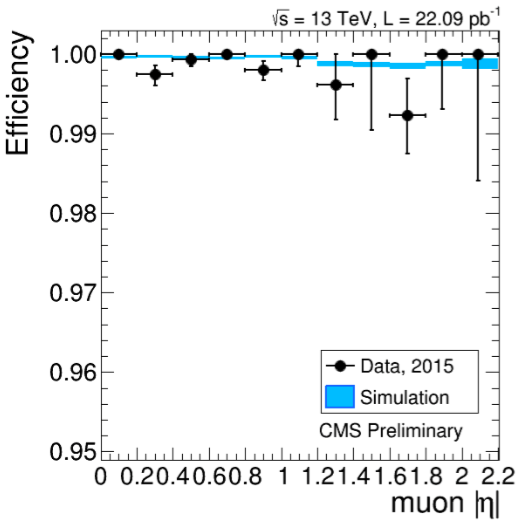
\includegraphics[width=0.38\textwidth]{\chsix/mu-reco-eff-eta.png}}
\subfigure[]{\label{fig:mu_reco_eff_b}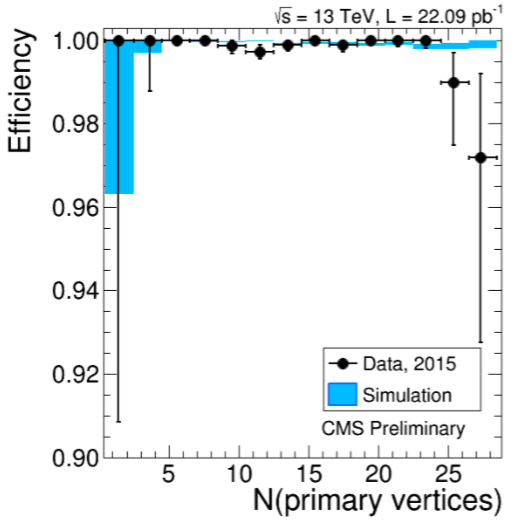
\includegraphics[width=0.38\textwidth]{\chsix/mu-reco-eff-PU.png}}
\caption{Tracking efficiency measured with a T\&P technique, for muons from Z decays, as a function of the muon $\eta$ (a) and the number of primary vertices (b), for 2015 data (black dots) and simulation (blue bands)~\cite{CMS-DP-2015-016}.}
\label{fig:mu_reco_eff}
\end{figure}

The combination of different algorithms provides robust and efficient muon reconstruction.
After the completion of both algorithms, the reconstructed standalone, global, and tracker muons are merged into a single software object, with the addition of further information, like isolation and energy collected in matching calorimeter towers. This information can be used for further identification, in order to achieve a balance between efficiency and purity of the muon sample as described in Section~\ref{subsec:muonid}.\\

The performance of the reconstruction for high-\pt muons is strongly affected by radiative processes and by the muon detector alignment. 
Electromagnetic showers and large energy losses can arise as the muon traverses the steel layers of the magnet return yoke, producing additional segments in the muon chambers.
These events can affect the measurement done in the muon detectors. Therefore, specialized reconstruction algorithms for high-\pt muons, known as ``TeV-muon'' refits, have been developed in CMS as described in the following.

The \textit{tracker-plus-first-muon-station} fit (TPFMS) only uses hits from the tracker and the innermost muon station with hits, to reduce the sensitivity to possible showering starting deeper in the muon system. The \textit{Picky} fit uses all tracker hits, while a selection is applied to muon hits. Hits from chambers with a high probability of shower contamination (determined from the hit occupancy) are required to be compatible with the extrapolated trajectory by applying a $\chi^2$ cut. The \textit{dynamic truncation} algorithm (DYT) starts from the idea that the muon track reconstruction should be stopped after a large energy loss, as hits produced after that can only bias the momentum measurement. For every global-muon trajectory the algorithm starts from the corresponding tracker track and propagates it out to the muon stations. Compatible segments (or hits) in the muon chambers are found by using an estimator which takes into account the propagation of the tracker covariance matrix through the material and the magnetic field, and the covariance matrices of the candidate muon segments (or hits).

Momentum assignment is then performed by the \textit{Cocktail} algorithm which combines the above methods to further improve the resolution at high \pt reducing the tails of the momentum resolution distribution.
In particular, the algorithm chooses, on a track-by-track basis, the best muon reconstruction. For Run~1, the Cocktail-algorithm decision is taken between the tracker-only, TPFMS, and Picky fits. 
This version of the algorithm is also known as the \textit{Tune P} algorithm. It starts with the Picky fit, then switches to the tracker-only fit if the goodness of fit ($\chi^2$/n.d.f.) of the latter is significantly better. Then it compares the $\chi^2$/n.d.f. of the chosen track with that of TPFMS; TPFMS is chosen if it is found to be better. For high-\pt muons, TPFMS and Picky algorithms are selected by Tune P in most of the cases, in approximately equal amounts, while the tracker-only fit is selected only in a few percent of events. 

For Run~2, the Tune P algorithm was extended to include also the DYT fit. The selection is still made on a track-by-track basis, but using both the $\chi^2$/n.d.f. of the track and the relative error of the \pt measurement. The algorithm starts with the Picky fit, then switches to DYT if the DYT track has a lower relative \pt error. It then compares the $\chi^2$/n.d.f. of the chosen track with that of the tracker-only fit and picks tracker-only if its $\chi^2$/n.d.f. is significantly better. Then the $\chi^2$/n.d.f. of the chosen track and TPFMS are compared and the one giving the best result is kept. At the end, if the final candidate track has \pt lower than 200\GeV or the tracker-only \pt is lower than 200\GeV, the tracker-only track is selected.%The momentum resolution obtained with this new optimized version of the Tune P algorithm, reaches 5.9\% for muons with \pt in the range $700 < \pt < 2000\GeV$, as measured with cosmic-ray muon data~\cite{Radogna:2205870}.

The momentum resolution obtained with the Tune P algorithm for muons with \pt in the range $350 < \pt < 2000\GeV$ is found to be $\approx$ 6\%, as measured with cosmic-ray muon data~\cite{Chatrchyan:2012xi,Radogna:2205870}.

%Specialized algorithms for high-energy muon reconstruction, known as ?TeV-muon? refits, have been developed in CMS and the final momentum assignment is performed by the so called ?Cocktail? algorithm which chooses the best muon track candidate. These algorithms have been updated and tuned to optimize the performance in collisions at 13 TeV.
%To further improve the resolution at high \pt, mainly by reducing the tails of the momentum resolution distribution, combinations of the above can be used. In particular, the Tune P al- gorithm chooses, on a muon-by-muon basis, between the tracker-only, TPFMS, and Picky fits. The algorithm starts with the Picky fit, then switches to the tracker-only fit if the goodness of fit of the latter is significantly better. Then it compares the goodness of fit of the chosen track with that of TPFMS; TPFMS is chosen if it is found to be better. For high-pT muons, TPFMS and Picky algorithms are selected by Tune P in most of the cases, in approximately equal amounts, while the tracker-only fit is selected only in a few percent of events

%%%%%%%%
\subsection{Muon trigger}\label{subsec:mutrigger}
%%%%%%%%

In the Level-1 muon trigger, muon candidates are identified by using hits in all three CMS muon detector systems: DT, CSC, and RPC.
It has a latency of 3.2\mus and reduces the rate of the readout of events with muon candidates
at the detector front-end electronics to a few kHz by applying selections on the estimated muon \pt and quality.
In the muon HLT, first a Level-1 trigger object is used as a seed to reconstruct a standalone-muon track in the muon system, leading to an improved \pt estimate. At this point, \pt threshold filters are applied to the standalone-muon (also called Level-2 muon). Then seeds in the inner tracker are generated in the region around the extrapolated Level-2 muon, and tracker tracks are reconstructed. If a successful match is made between a tracker track and the Level-2 muon, a global fit combining tracker and muon hits is performed, yielding a Level-3 muon track on which the final \pt requirements are applied. In this way, the rate of recorded inclusive muon events is reduced to a few tens of Hz. The average processing time of the HLT reconstruction is about 50\unit{ms}.

The L1 and HLT trigger used to collect the data analyzed in this thesis are listed in Tables~\ref{tab:triggMu8TeV} and~\ref{tab:triggMu13TeV} for the 8 and 13\TeV data analysis, respectively.
For both analyses the HLT used to select the events is the unprescaled single-muon trigger with the lowest \pt threshold that does not include muon isolation requirements. 
%Both analyses requires one muon candidate. The HLT used to select the events is the unprescaled single-muon trigger with the lowest \pt threshold that does not include muon isolation requirements.
In fact, although muons produced in the leptonic decays of high-\pt W bosons tend to be isolated, their high momentum enhances the production of electromagnetic showers, that can mimic a non-isolated muon candidate.
Therefore, only requirements on the muon \pt and $\eta$ are applied at this stage.
As the very forward region, $2.1 < |\eta| < 2.4$, is characterized by higher rates of low-\pt muons, the muon candidate is required to have $|\eta| < 2.1$, so preventing a too high trigger rate while keeping a reasonably low \pt threshold.
The final states under study here are characterized by centrally produced muons so that the probability of signal events with muons in the very forward region is negligible.
The efficiency of the L1 single-muon trigger with the 16\GeV threshold is shown in Fig.~\ref{fig:mu_L1trigg} as a function of the offline reconstructed muon \pt and $\eta$. In 2012 the efficiency for this trigger was greater than 90\%. A similar result is obtained in 2015.
%The efficiency at the plateau is 2% lower in 2012 with respect to 2011 due to an optimization aimed to reduce the single muon trigger rate by 50% which allowed to keep pT thresholds for 2012 running as low as the ones used for 2011. In both 2011 and 2012 the efficiency of the L1 single muon trigger was greater than 90%.

\begin{table}[!htb]
\centering
\caption{The L1 and HLT single-muon triggers used to collect the 8\TeV data analyzed in this thesis together with the imposed requirements on the muon candidate.}
\begin{tabular}{ l | c | c }
Trigger & Name & Selections\\
\hline
\hline
\multirow{3}{*}{Level 1} & \multirow{3}{*}{L1\_SingleMu16\_eta2p1}                 & 1 muon candidate with:\\ 
                                     &                                                                                   & \pt $>$ 16\GeV\\
                                     &                                                                                   & $|\eta| <$ 2.1\\
\hline
\multirow{3}{*}{HLT} & \multirow{3}{*}{HLT\_Mu40\_eta2p1} & 1 global muon with:\\
                                &                                                            & \pt $>$ 40\GeV\\
                                &                                                            & $|\eta| <$ 2.1\\
\hline 
\end{tabular}
\label{tab:triggMu8TeV}
\end{table}

\begin{table}[!htb]
\centering
\caption{The L1 and HLT single-muon triggers used to collect the 13 TeV data analyzed in this thesis together with the imposed requirements on the muon candidate.}
\begin{tabular}{ l | c | c }
Trigger & Name & Selections\\
\hline
\hline
\multirow{2}{*}{Level 1} & \multirow{2}{*}{L1\_SingleMu25}  & 1 muon candidate with:\\ 
                                     &                                                       & \pt $>$ 25\GeV\\
\hline
\multirow{3}{*}{HLT} & \multirow{3}{*}{HLT\_Mu45\_eta2p1} & 1 global muon with:\\
                                &                                                            & \pt $>$ 45\GeV\\
                                &                                                            & $|\eta| <$ 2.1\\
\hline 
\end{tabular}
\label{tab:triggMu13TeV}
\end{table}

\begin{figure}[!htb]
\centering
\subfigure[]{\label{fig:mu_L1trigg_a}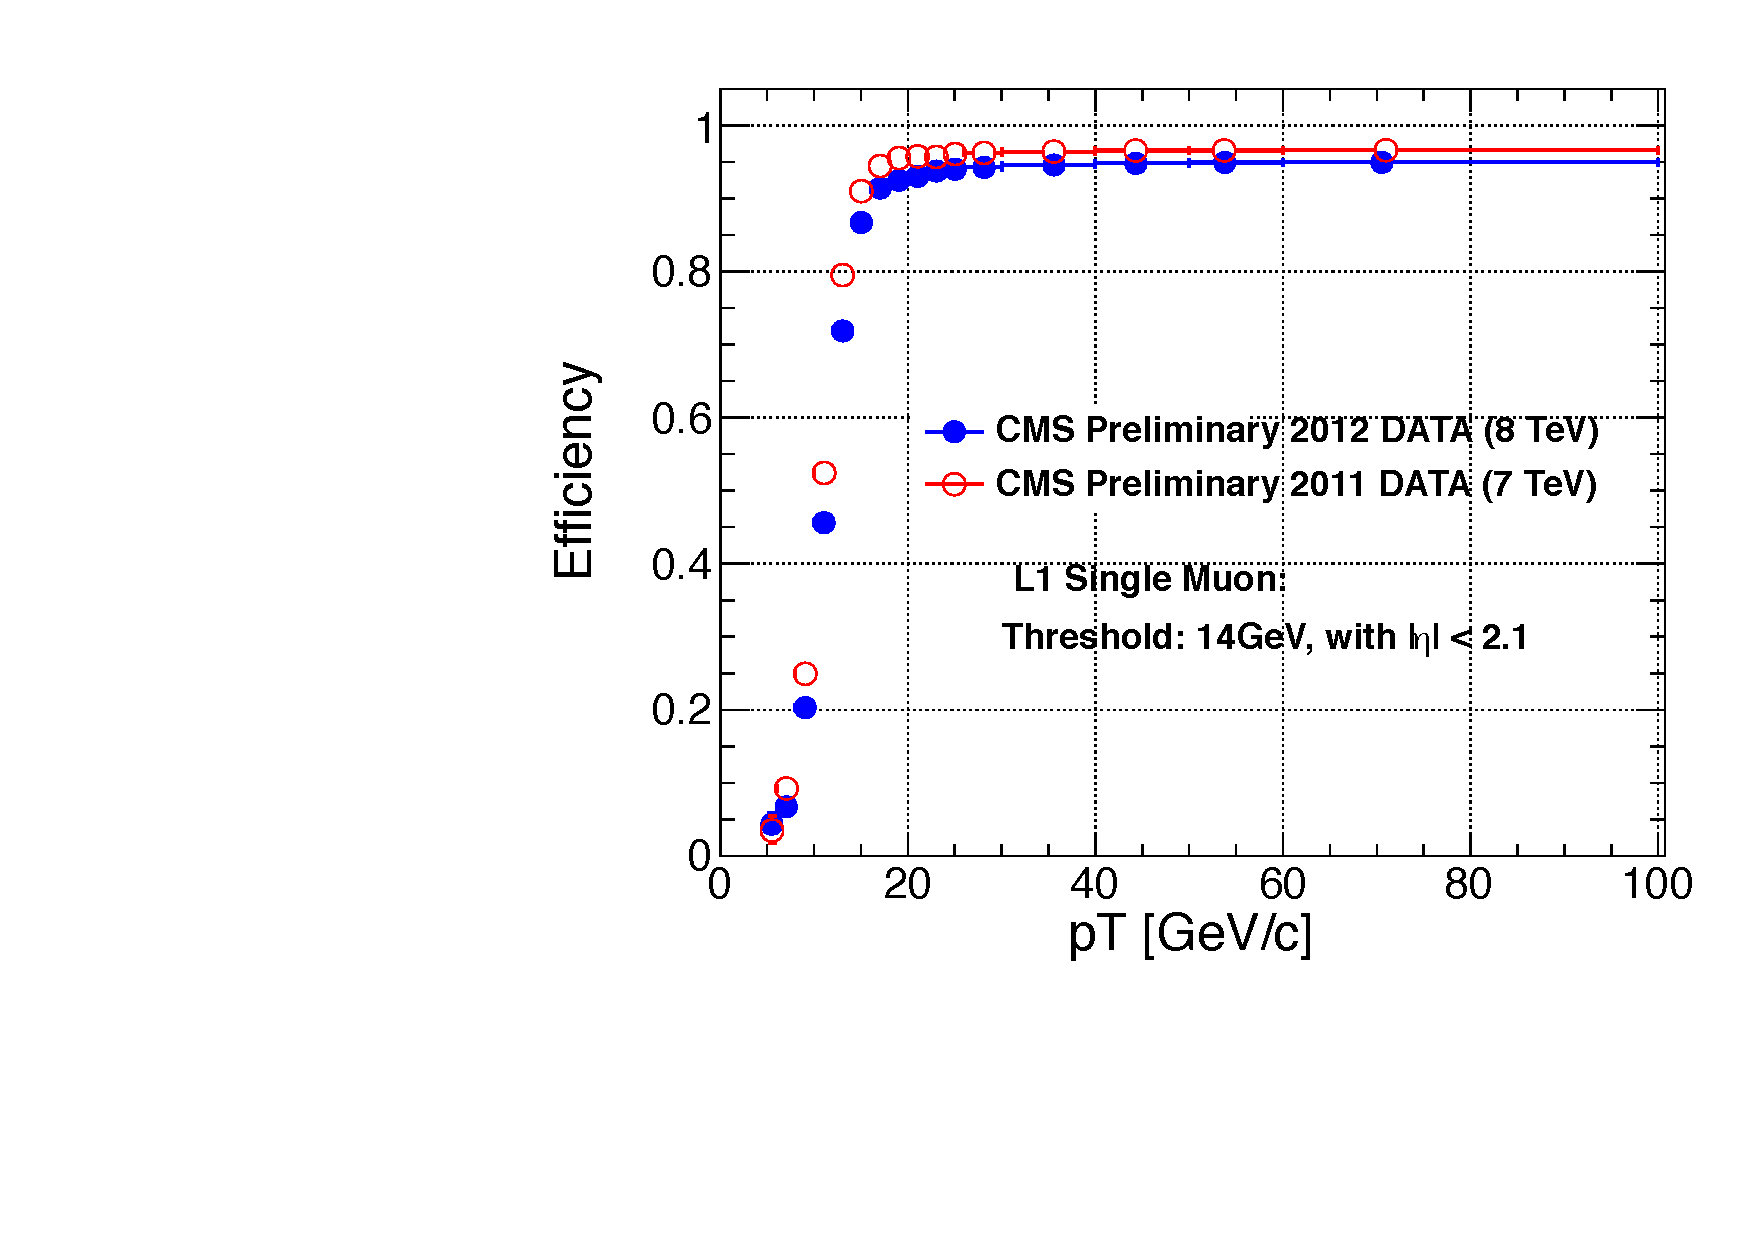
\includegraphics[width=0.45\textwidth]{\chsix/SingleMu16_pt.pdf}}
\subfigure[]{\label{fig:mu_L1trigg_b}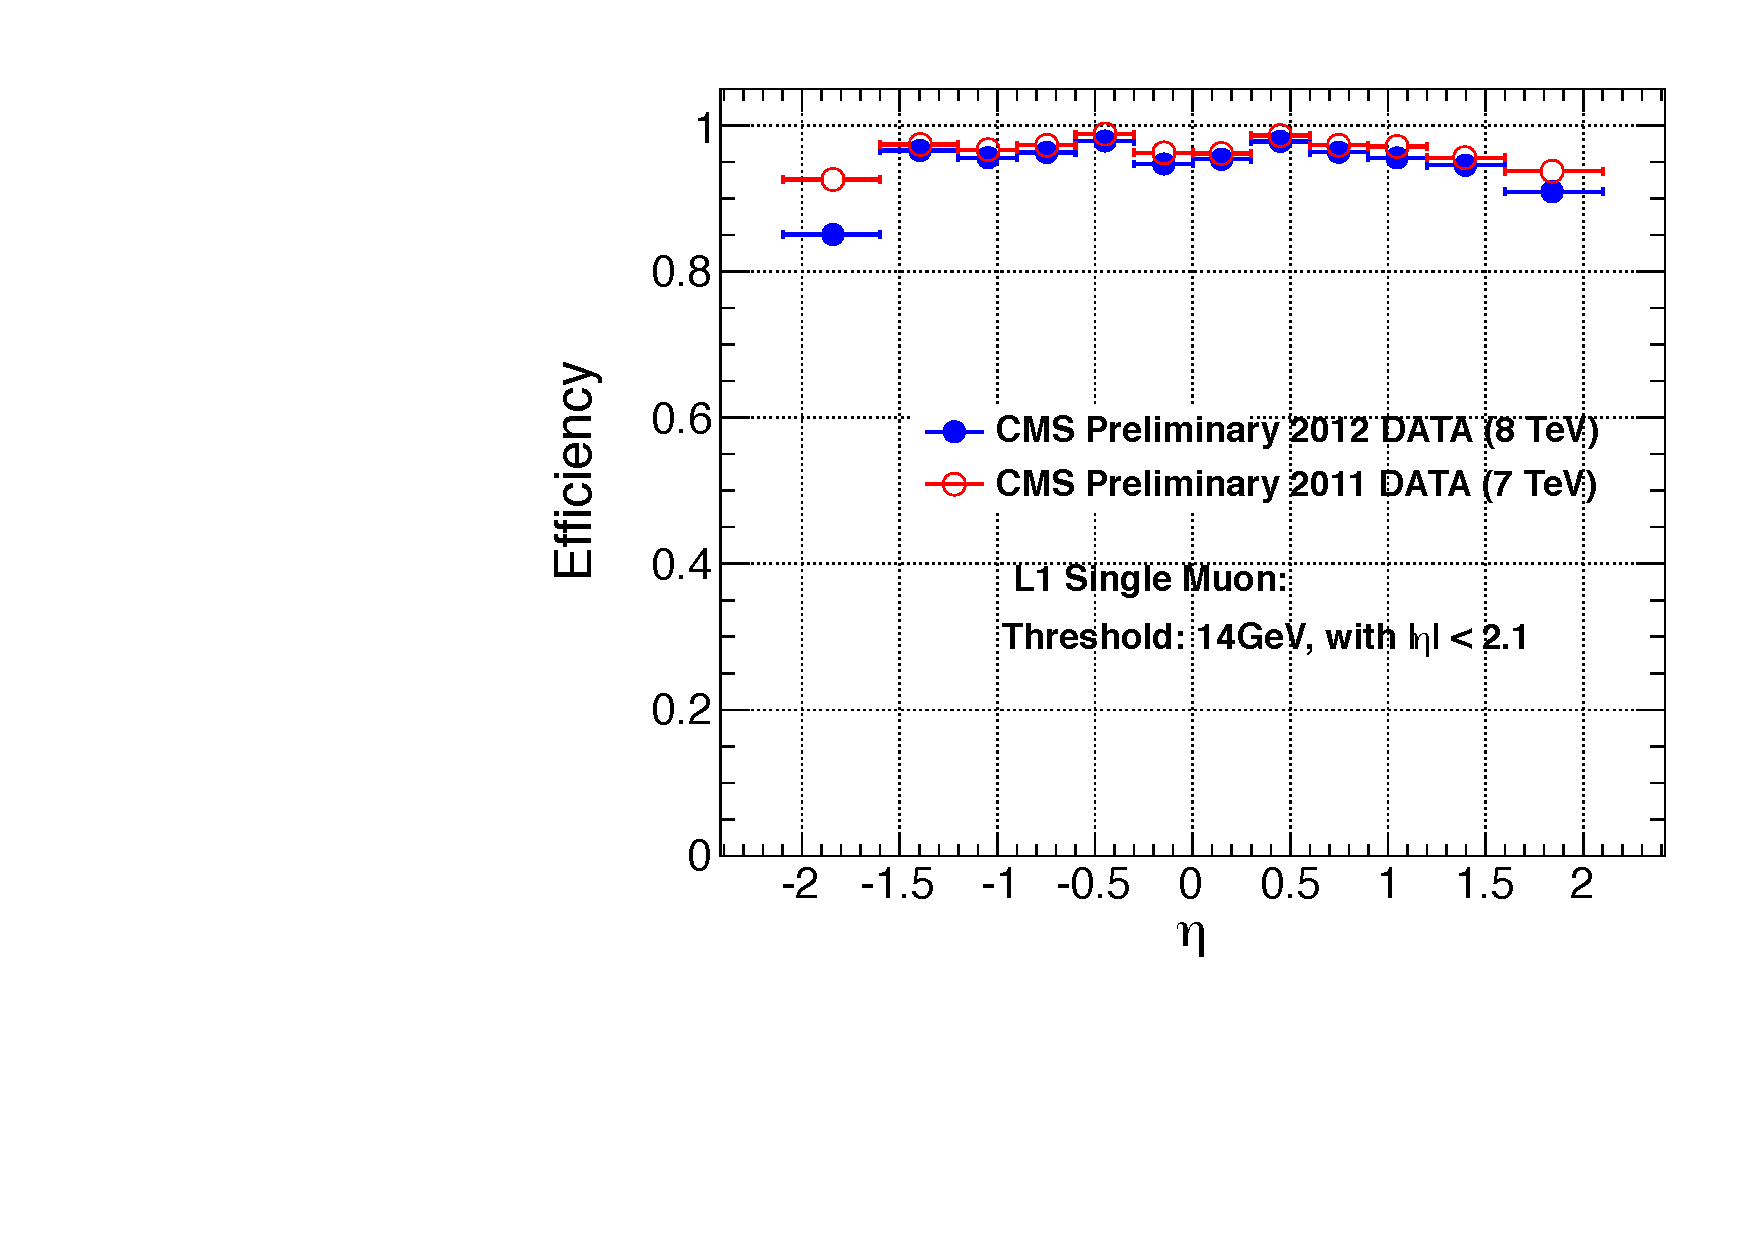
\includegraphics[width=0.45\textwidth]{\chsix/SingleMu16_eta.pdf}}
\caption{Efficiency of the L1 single-muon trigger with a threshold of 14\GeV on the muon \pt as a function of the muon \pt (a) and $\eta$ (b)~\cite{Brooke:1496888}.}
\label{fig:mu_L1trigg}
\end{figure}

%The offline reconstructed \pt of the muons must be greater than 50 (53) GeV for the 8 (13) TeV analysis, where the trigger reaches the plateau. Furthermore the selected muon must be reconstructed within $|\eta|$ < 2.1 as a consequence of the trigger criteria.
The efficiency for a muon passing the high-\pt selections described in Section~\ref{subsec:muonid} to fire the HLT single-muon triggers have been measured in data with T\&P method and are summarized in Tables~\ref{tab:hltMueff8TeV} and~\ref{tab:hltMueff13TeV}. 

\begin{table}[!htb]
\centering
\caption{Efficiencies and scale factors for the single-muon HLT trigger used in the 8\TeV data analysis
for muons with \pt $>$ 50\GeV, $|\eta| <$ 2.1, and satisfying the high-\pt and isolation selections described in Section~\ref{subsec:muonid}.
The quoted uncertainties are statistical.}
\begin{tabular}{ c | c | c | c}
 & $0 < |\eta| < 0.9$ & $0.9 < |\eta| < 1.2$ & $1.2 < |\eta| < 2.1$\\
\hline
\hline
Efficiency simulation & 95.10\% $\pm$ 0.03\% & 87.01\% $\pm$ 0.03\% & 81.56\% $\pm$ 0.03\%\\
Efficiency data & 92.90\% $\pm$ 0.02\% & 83.14\% $\pm$ 0.06\% & 80.27\% $\pm$ 0.05\%\\
Data/simulation scale factor & 0.9768 $\pm$ 0.0004 & 0.956 $\pm$ 0.001 & 0.984 $\pm$ 0.001\\
\hline 
\end{tabular}
\label{tab:hltMueff8TeV}
\end{table}
%https://twiki.cern.ch/twiki/bin/viewauth/CMS/MuonReferenceEffs
%https://indico.cern.ch/event/257000/contributions/1586340/attachments/451105/625487/SingleMuTriggerEff_10June_updated.pdf

\begin{table}[!htb]
\centering
\caption{Efficiencies and scale factors for the single-muon HLT trigger used in the 13\TeV data analysis
for muons with \pt $>$ 53\GeV, $|\eta| <$ 2.1, and satisfying the high-\pt and isolation selections described in Section~\ref{subsec:muonid}.
The quoted uncertainties are statistical.}
\begin{tabular}{ c | c | c | c}
 & $0 < |\eta| < 0.9$ & $0.9 < |\eta| < 1.2$ & $1.2 < |\eta| < 2.1$\\
\hline
\hline
Efficiency simulation & 97.6\% $\pm$ 0.1\% & 93.4\% $\pm$ 0.4\% & 94.8\% $\pm$ 0.2\%\\
Efficiency data & 94.6\% $\pm$ 0.2\% & 89.7\% $\pm$ 0.4\% & 91.8\% $\pm$ 0.2\%\\
Data/simulation scale factor & 0.969 $\pm$ 0.002 & 0.961 $\pm$ 0.006 & 0.968 $\pm$ 0.003\\
\hline 
\end{tabular}
\label{tab:hltMueff13TeV}
\end{table}
%https://twiki.cern.ch/twiki/bin/view/CMS/MuonReferenceEffsRun2
%https://indico.cern.ch/event/462268/contributions/1979019/attachments/1188638/1724574/2015.11.17_MuonPOG_SingleMuTrigEff_SF_KPLee_v2.pdf

%%%%%%%%
\subsection{Muon identification}\label{subsec:muonid}
%%%%%%%%

The standard CMS muon reconstruction provides additional information for each muon, useful for muon quality selection and identification in physics analyses~\cite{Chatrchyan:2012xi}. 
In general, particles detected as muons are produced in pp collisions from different sources which lead to different experimental signatures. The so-called \textit{prompt muons} arise either from decays of W, Z, or promptly produced quarkonia states. Real muons are also produced in the decay of heavy flavour particles, such as beauty or charmed mesons, as well as in light hadron (pions or kaons) decays. Less frequently, muons might originate from a calorimeter shower or from a nuclear interaction in the detector. Furthermore, the so called ``punch-through'' effect, i.e. hadron shower remnants penetrating through the calorimeters and reaching the muon system, can lead to the reconstruction of a muon candidate. Most of the physics analyses in CMS studying SM processes or searching for BSM signals use prompt muons, while all the other categories of muons constitute the background. These analyses exploit the same set of information, although the applied selections might be different depending on the signature of interest and the expected background. In this section only the specific selection developed for high-\pt muons is described. One of the main difference with respect to the low- and medium-\pt muon selection is that this particular identification procedure does not use the PF algorithm. It is aimed at the best reconstruction of the muon track parameters without relying on external information on the event. Moreover, the goodness of the global-muon track fit selection, based on the $\chi^2$ of the track, is not requested, but an additional selection based on the relative \pt resolution for the track used for momentum determination is applied. 

The high-\pt muon selection criteria are described in the following and they have not been changed since Run~1:

\begin{itemize}
\item The muon must be reconstructed both as a tracker and a global muon. This is effective against decays in flight, punch through and accidental matching (with noisy or background tracks or segments).
%\item The number of hits in the tracker track part of the muon. Generally tracks with small number of hits give bad pT estimate. In addition decays in flight give rise in many cases to lower hit occupancy in the tracks.
\item Number of pixel hits in the tracker track $\geq$ 1. To further suppress muons from decays in flight.
%\item There should be at least one pixel hit in the tracker track part of the muon. The innermost part of the tracker is an important handle to discard non-prompt muons. By requiring just a minimal number of hits we introduce negligible reconstruction inefficiency.
\item Number of tracker layers involved in the track measurement $\geq$ 6. This guarantees a good \pt measurement, for which some minimal number of measurement points in the tracker is needed. It also suppresses muons from decays in flight.
\item Number of muon-chamber hits included in the global-muon track fit $\geq$ 1. This requirement assures that the global muon is not an accidental match between the information from the muon system and the tracker. This could happen in particular for non-prompt muons or fake muons from punch through.
%\item The global muon has to contain at least one ?valid? muon hit. This re- quirement assures that the global muon is not a ?bad? match between the information from the muon system and the tracker. This could happen in particular for non-prompt muons.
\item The muon track is required to have muon segments in at least 2 muon stations to further suppress punch through and accidental track-to-segment matches. This selection is furthermore consistent with the logic of the single-muon trigger, which requires segments in at least two muon stations to obtain a meaningful estimate of the muon \pt.
%\item The muon track has to have a minimum number (2) of chamber hits in different stations with matching (consistent with the propagated to the muon chambers tracker track) segments. This is also to comply with a similar looser requirement in the trigger.
%\item Very bad fits are rejected by requiring reasonable global muon fit quality. If there is a decay in flight inside the tracking volume, the trajectory could contain a sizeable ?kink?, resulting in a poorer  2 of the fit used to determine the trajectory.
\item Transverse impact parameter of the muon track $< 2\mm$. This assures the compatibility of the muon track with the interaction point hypothesis and it is effective against cosmic background and further suppress muons from decays in flight.
\item Longitudinal impact parameter of the muon track $< 5\mm$. To further suppress cosmic muons, muons from decays in flight and tracks from pileup.
%\item Muon can be required also to be matched a Particle Flow (PF) muon. PF is a reconstruction technique widely used in CMS analyses. It makes use of the full detector information to describe the global collision event, by identifying particles individually and clustering them into more complex objects. More details about PF algorithm are available in [49,50].
\item Relative \pt error $< 30\%$. To further suppress misreconstructed muons.
\end{itemize}

In addition to these identification criteria, an isolation requirement is applied to the well-identified muons. In particular, the muon must pass a relative tracker-only isolation selection: the scalar sum of the \pt of all other tracks in a cone of  $\Delta R < 0.3$ around but not including the muon tracker track must be less than 10\% of the muon \pt, also as measured by the tracker. To be used in the calculation of the tracker-based isolation, tracks have to be within 2\mm, in the $z$ direction, of the primary vertex with which the muon candidate is associated. These additional criteria help suppress the effect of tracks originating from pileup on the reconstructed quantities.

The efficiency and data-to-simulation scale factors for the high-\pt muon identification and isolation criteria measured with the T\&P method in 8 and 13\TeV data are summarized, respectively, in Tables~\ref{tab:idMueff8TeV} and~\ref{tab:idMueff13TeV}. The scale factors are close to unity, indicating a good agreement between data and simulation. They are used in the analyses presented in this thesis to correct the normalization of simulations.

\begin{table}[!htb]
\centering
\caption{Efficiencies and scale factors for the high-\pt muon identification and isolation criteria used in the 8\TeV data analysis for muons with $\pt > 50\GeV$ and $|\eta| < 2.1$.}
\begin{tabular}{ l | c | c | c}
Muon $|\eta|$ & $0 < |\eta| < 0.9$ & $0.9 < |\eta| < 1.2$ & $1.2 < |\eta| < 2.1$\\
\hline
\hline
 & \multicolumn{3}{c}{High-\pt muon identification}\\
\hline
Efficiency simulation & 96.51\% $\pm$ 0.02\% & 96.61\% $\pm$ 0.04\% & 95.54\% $\pm$ 0.03\%\\
Efficiency data & 95.54\% $\pm$ 0.02\% & 95.87\% $\pm$ 0.04\% & 95.06\% $\pm$ 0.03\%\\
Data/simulation scale factor & 0.9900 $\pm$ 0.0003 & 0.992 $\pm$ 0.001 & 0.9949 $\pm$ 0.0004\\
\hline
 & \multicolumn{3}{c}{Tracker-based muon isolation}\\
\hline
Efficiency simulation & 99.49\% $\pm$ 0.01\% & 99.58\% $\pm$ 0.01\% & 99.59\% $\pm$ 0.01\%\\
Efficiency data & 99.46\% $\pm$ 0.01\% & 99.51\% $\pm$ 0.01\% & 99.56\% $\pm$ 0.01\%\\
Data/simulation scale factor & 0.9996 $\pm$ 0.0001 & 0.9994 $\pm$ 0.0001 & 0.9997 $\pm$ 0.0001\\
\hline 
\end{tabular}
\label{tab:idMueff8TeV}
\end{table}
%https://twiki.cern.ch/twiki/bin/viewauth/CMS/MuonReferenceEffs
%https://indico.cern.ch/event/257630/contributions/577156/attachments/452667/627631/Final_MuonID_and_Iso_eff_ReReco-22Jan2013.pdf

\begin{table}[!htb]
\centering
\caption{Efficiencies and scale factors for high-\pt muon identification and isolation criteria used in the 13\TeV data analysis for muons with $\pt > 53\GeV$ and $|\eta| < 2.1$.}
\begin{tabular}{ l | c | c }
Muon $|\eta|$ & $0 < |\eta| < 1.2$ & $1.2 < |\eta| < 2.1$\\
\hline
\hline
 & \multicolumn{2}{c}{High-\pt muon identification}\\
\hline
Efficiency simulation & 97.6\% $\pm$ 0.2\% & 99.81\% $\pm$ 0.2\%\\
Efficiency data & 96.7\% $\pm$ 0.4\% & 1.0\% $\pm$ 0.7\%\\
Data/simulation scale factor & 0.991 $\pm$ 0.005 & 1.002 $\pm$ 0.007\\
\hline
 & \multicolumn{2}{c}{Tracker-based muon isolation}\\
\hline
Efficiency simulation & 99.8\% $\pm$ 0.1\% & 99.6\% $\pm$ 0.1\%\\
Efficiency data & 99.7\% $\pm$ 0.1\% & 99.7\% $\pm$ 0.1\%\\
Data/simulation scale factor & 0.999 $\pm$ 0.001 & 1.001 $\pm$ 0.001\\
\hline
\end{tabular}
\label{tab:idMueff13TeV}
\end{table}
%https://twiki.cern.ch/twiki/bin/view/CMS/MuonReferenceEffsRun2
%https://indico.cern.ch/event/465390/contributions/1141124/attachments/1197504/1741010/Lanyov_Highpt_eff_TnP_01.12.2015.pdf

%%%%%%%%%%
%\section{Jets}\label{sec:jets}
 %%%%%%%%%%%%%%%%%%%%%%%%%%%%%%%%%%%%%%%%%%%%%%%%%%%%%%%%%%%%%%%
\section{Jets}\label{sec:jets}
%%%%%%%%%%%%%%%%%%%%%%%%%%%%%%%%%%%%%%%%%%%%%%%%%%%%%%%%%%%%%%%

Quarks and gluons produced in the high-energy processes
such as hard scattering of partons in pp collisions, carry a color charge and 
%Particles carrying a color charge, such as quarks,
cannot exist in free form because of QCD confinement which only allows for colorless states (Section~\ref{subsec:QCD}).
%Quarks and gluons interact with pairs of quarks and anti-quarks produced from the vacuum until the formation of stable colourless hadrons.
At detector level, only the ensemble of the final colourless stable hadrons, simulated by the parton shower algorithms, can be observed.
This exhibits as a jet of collimated particles which reflects the energy and the flight direction of the initial parton.
Therefore, a jet is a cluster of charged particle tracks and calorimetric energy deposits in the detector, whose properties depend on the algorithm used for its definition.
%The ensemble of the final colourless objects is called a \textit{jet} and it is reconstructed in the detector from energy depositions and charged particle momenta.
%The jets point back to the primary interaction, i.e. to the partons the jets originated from, but a correction for hadronization and detector effects is needed.
The jet-clustering algorithms cluster particles (at parton, particle or detector level) into jets and reconstruct the energy and direction of the original parton. The task of a jet-clustering algorithm is to allow comparisons between theoretical predictions, which are usually described by perturbative calculations, and experimental data. This is achieved by reducing the complex structure of particle jets from a scattered parton to a simple four-momentum, which represents the main property of particle jets.
In order to guarantee a meaningful calculation of theory predictions, jet-clustering algorithms are characterized by two important properties.
%Two properties of jet clustering algorithms are desired to be able to calculate meaningful theory predictions.
Clustering algorithms need to be infrared-safe, which means that the emission of infinitesimally-low-energy partons from partons inside a jet does not affect the jet properties. Furthermore, they need to be collinear-safe, which means that jet properties are not affected by the splitting of a parton inside a jet into two collinear partons.
Jet algorithms for hadron colliders can be divided into two classes: cone~\cite{Salam:2007xv} and sequential clustering~\cite{Catani:1993hr,Ellis:1993tq,Dokshitzer:1997in,Wobisch:1998wt,Cacciari:2008gp} algorithms.
%Jet algorithms for hadron colliders can be divided into two classes. One possibility is based on proximity in coordinate space, cone jet algorithms [180, 181]) whereas the other uses proximity in momentum space by successively merging pairs of particles in order of increasing relative transverse momentum, kT algorithms [182, 183]). For this work only the anti-kT algorithm of the kT family is used and detailed in the following.
The main algorithms used by LHC experiments belong to the second class and are the anti-$k_t$~\cite{Cacciari:2008gp} (AK) and the Cambridge--Aachen (CA)~\cite{Catani:1993hr,Dokshitzer:1997in} algorithms. In fact, they are found to fulfill theoretical requirements and to exhibit good properties for experimental measurements. For this work both algorithms are used and described in the following.
 
 %%%%%%%% 
\subsection{Jet-clustering algorithms}\label{subsec:jetsalgo}
%%%%%%%%

In sequential jet-clustering algorithms, jets are defined through sequential, iterative procedures that combine four-vectors of input pairs of particles until certain criteria are satisfied and jets are formed. In particular, for each pair of particles $i$ and $j$, a distance variable between the two particles ($d_{ij}$), and the so-called ``beam distance'' for each particle ($d_{iB}$), are computed:
 
\begin{equation}\label{eqn:jetalgo}
d_{ij} = \mathrm{min}(p_{Ti}^{2n},p_{Tj}^{2n})\frac{\Delta R^2_{ij}}{R^2}\quad,\quad\quad\quad
d_{iB} = p_{Ti}^{2n}\quad,
\end{equation} 

\noindent where $p_{Ti}$ and $p_{Tj}$ are the transverse momenta of particles $i$ and $j$, respectively, ``min'' refers to the smaller of the two \pt values, the integer $n$ depends on the specific jet algorithm, $\Delta R^2_{ij}$ is the distance between $i$ and $j$ in the $\eta$-$\phi$ plane, and $R$ is a free distance parameter, with all angles expressed in radians. The particle pair ($i$, $j$) with smallest $d_{ij}$ is combined into a single object. All distances are recalculated using the new object, and the procedure is repeated until, for a given object $i$, all the $d_{ij}$ are greater than $d_{iB}$. Object $i$ is then classified as a jet and not considered further in the algorithm. The process is repeated until all input particles are clustered into jets.

The distance parameter $R$ is responsible for defining the angular size of the jet. The parameter $n$ governs the topological properties of the jets and, depending on its value, three different classes of clustering algorithms are distinguished. For $n = 1$ the procedure is referred to as the $k_t$ algorithm (KT)~\cite{Cacciari:2008gp}, which clusters soft objects before harder ones are added to the final jet, mimicking in reverse the parton fragmentation and gluon emission processes. For this reason, the algorithm tends to construct jets of irregular shapes which depend on the detailed distribution of soft particles in an event.
In addition, they are sensitive to the presence of low-\pt pileup contributions.
%The KT jets tend to have irregular shapes and are especially useful for reconstructing jets of lower momentum. For this reason, they are also sensitive to the presence of low-\pt pileup contributions.
%, and are used to compute the mean \pt per unit area of an event.
For $n = 0$, the procedure corresponds to the CA algorithm. This relies only on angular information, and, like the KT algorithm, provides irregularly-shaped jets. The CA and KT algorithms are useful in identifying jet substructure as described in Chapter~\ref{ch:vtagging}.
%The C-A algorithm still reflects aspects of the QCD parton shower, in particular the angular ordering of emissions. However, it is less directly relatedtothestructureofQCDpartonsplittingfunctionsthanthekT algorithmis,and represents a compromise between reflecting the structure of the parton shower and maintaining some insensitivity to soft radiation.
For $n = -1$, the procedure corresponds to the AK algorithm, which compares the inverse square of the transverse momenta.
The AK algorithm is used extensively in LHC experiments and by the theoretical community for finding well-separated jets. The use of the inverse square of the \pt as a weight in the $d_{ij}$ distances has the advantage that hard objects collect adjacent soft ones before these are clustered among themselves into harder object. %This means that the most energetic cores of jets are found first.
%, figuratively reproducing in reverse the parton fragmentation and gluon emission processes. --> not true! harder objects come first in QCD splitting.
This property makes the algorithm independent on soft radiation, preserving infrared-safety. Low-energy gluons emitted at large angles are picked up by the algorithm rather late in the clustering process and therefore do not affect the jet properties. They are picked up after all hard emissions at small angles and before two soft particles can cluster with each other. Soft emissions will therefore not cluster into separate jets, preserving infrared-safety. The AK algorithm is also collinear-safe as the clustering is driven by the angular distance between two particles. Furthermore, as soft particles clustered later have a minimal impact on the larger four-momentum of the jet core, the AK algorithm tends to cluster particles out to distances $R$ from the core of a jet, yielding very regular jets. This allows for straight-forward calibration and understanding of the detector acceptance. The behaviours of the CA and AK jet algorithms are illustrated in Fig.~\ref{fig:jetalgos}. 
%this algorithm tends, by construction, to form almost circular jets allowing for straight-forward calibration and understanding of the detector acceptance. The behaviours of the CA and AK jet algorithms are illustrated in Fig.~\ref{fig:jetalgos}. 
%As soft particles clustered later have a minimal impact on the larger four-momentum of the jet core, the anti-kT algorithm tends to cluster particles out to distances R from the core of a jet, yielding very regular jets.
%This algorithm is collinear-safe as the clustering is driven by the angular distance between two particles. Gluons emitted at small angles are picked up by the algorithm in early steps of the iteration and therefore do not affect the jet properties. The algorithm is also infrared-safe. Due to the weighting with the inverse maximum squared transverse momentum, the emission of additional low energy gluons are picked up rather late in the clustering process. They are picked up after all hard emissions at small angles, but, importantly, before two soft particles can cluster with each other. Soft emissions will therefore not cluster into separate jets, preserving infrared-safety.
%The AK algorithm has very good experimental properties. By construction it tends to form almost circular jets with a radius of R. This is demonstrated for an example event in Fig. 7.1. Only if two jets are closer than 2R, the shape of the two jets varies from being circular. Experimentally this feature is very important as it allows straight-forward calibration and un- derstanding of the detector acceptance. Due to its limited cone size, the measurement of jets can be restricted to active detector regions. Due to the fixed cone size, the number of detector cells to be clustered into a jet is constant over certain detector regions and therefore straight-forward to calibrate.

\begin{figure}[!htb]
\centering
\subfigure[]{\label{fig:jetalgos_a}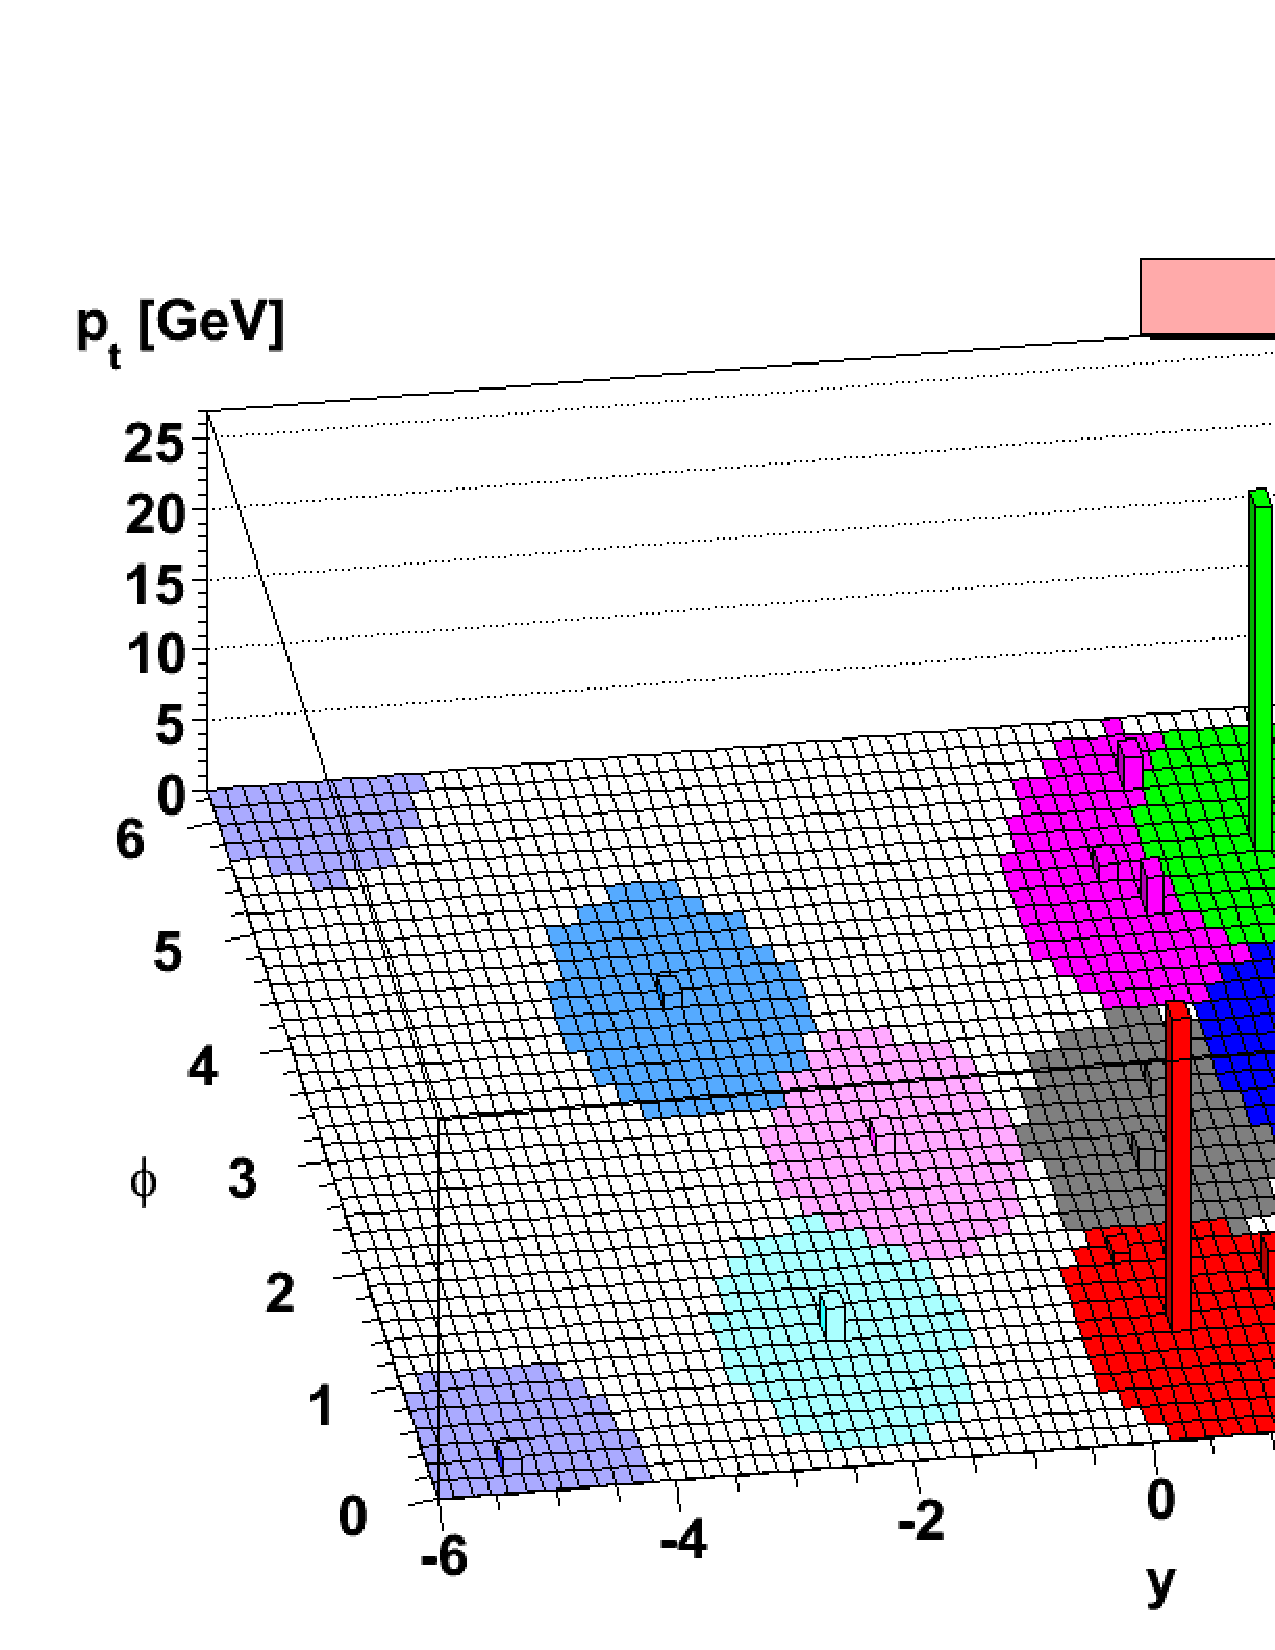
\includegraphics[width=0.45\textwidth]{\chsix/herwig-parton-level-ev-antikt-R1p0-ghosted4root.pdf}}
\subfigure[]{\label{fig:jetalgos_b}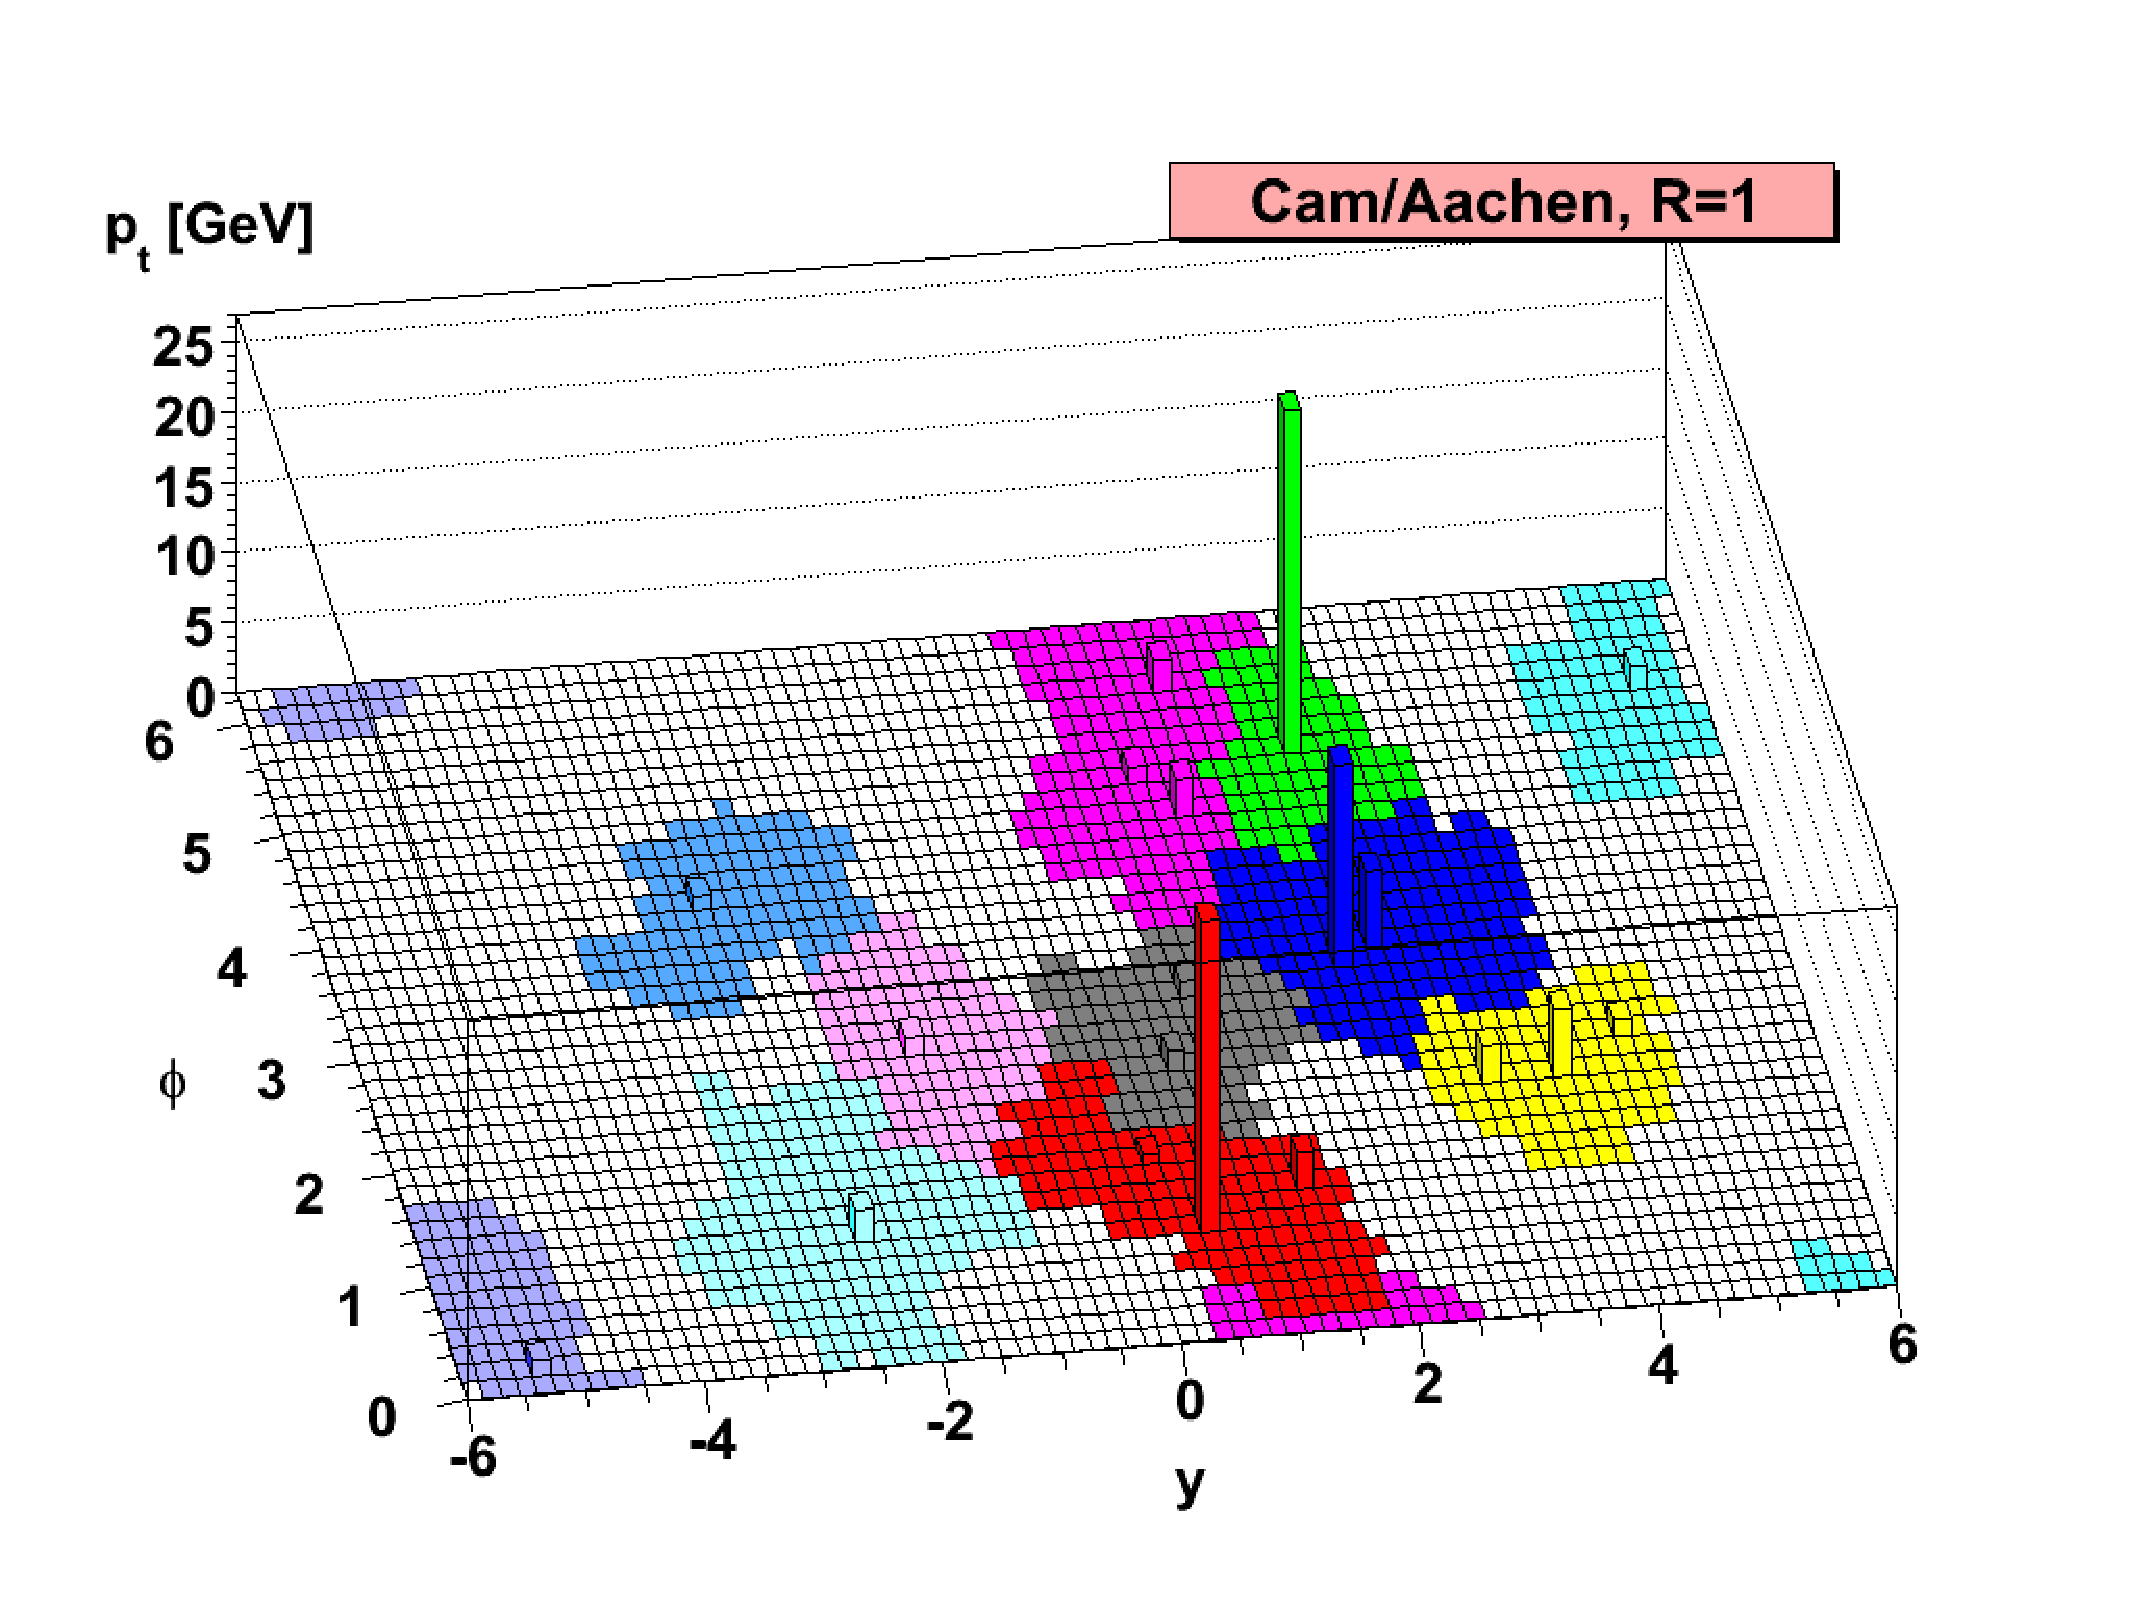
\includegraphics[width=0.45\textwidth]{\chsix/herwig-parton-level-ev-cam-R1p0-ghosted4root.pdf}}
\caption{An example of jet-clustering with the AK (a) and CA (b) algorithms. The reconstructed jets are shown as colored regions~\cite{Cacciari:2008gp}.}
\label{fig:jetalgos}
\end{figure}

The choice of the distance parameter $R$ generally depends on the analysis. While large cone-size jets collect all energy from the scattered parton, they also pick up a large contribution of background energy from the underlying event or pileup interactions. Small cone-size jets pick up little contamination, but may not collect all energy from the scattered parton. 
The default choice in CMS for physics analyses in Run~1 and Run~2 uses the AK algorithm with $R = 0.5$ (AK5) and $R = 0.4$ (AK4), respectively, since more collimated jets are expected at higher $\sqrt{s}$. The AK5 or AK4 algorithms are used in this analysis to put requirements on additional b jets in the event selection (Section~\ref{sec:finalselection}), along with the b-tagging algorithm described in Section~\ref{subsec:bjets}.

A larger value of $R$ increases the efficiency to entirely reconstruct the highly energetic products in the decays into hadrons of boosted V and Higgs bosons.
In fact, the average angular distance between the decay products is inversely proportional to the \pt of the mother particle. The default choice in CMS for physics analyses involving boosted V or Higgs bosons decaying hadronically is $R = 0.8$. In particular, CA8 and AK8 jets are used for Run~1 and Run~2 data analyses, respectively. The chosen value of $R$ provides a high efficiency for V or Higgs bosons with small boost and ensures that no efficiency is lost in the transition from the classical reconstruction in two small jets at low boson \pt to the reconstruction as a single large-cone jet at higher values. Another point to consider when choosing the value of $R$ is the \ttbar data sample available for validating highly boosted W jets (Section~\ref{sec:vtagging}). If $R$ is chosen too large, the b quark from the $\cPqt\to\PW\cPqb$ decay tends to merge into the W jet. The chosen value of $R$ is the result of a compromise between high efficiency for V or Higgs bosons with small boost and a sufficiently large sample of W jets in \ttbar data for validating the boosted boson jet identification procedure. Figure~\ref{fig:ca8effVsPt} shows the \pt range of W bosons for which the CA8 algorithm is efficient and compares this to the efficiency for reconstructing W bosons from two AK5 jets. Above a \pt of 200\GeV, the CA8 jet algorithm, used to identify W jets, becomes more efficient than the reconstruction of a W boson from two AK5 jets.

\begin{figure}[!htb]
 \begin{center}
  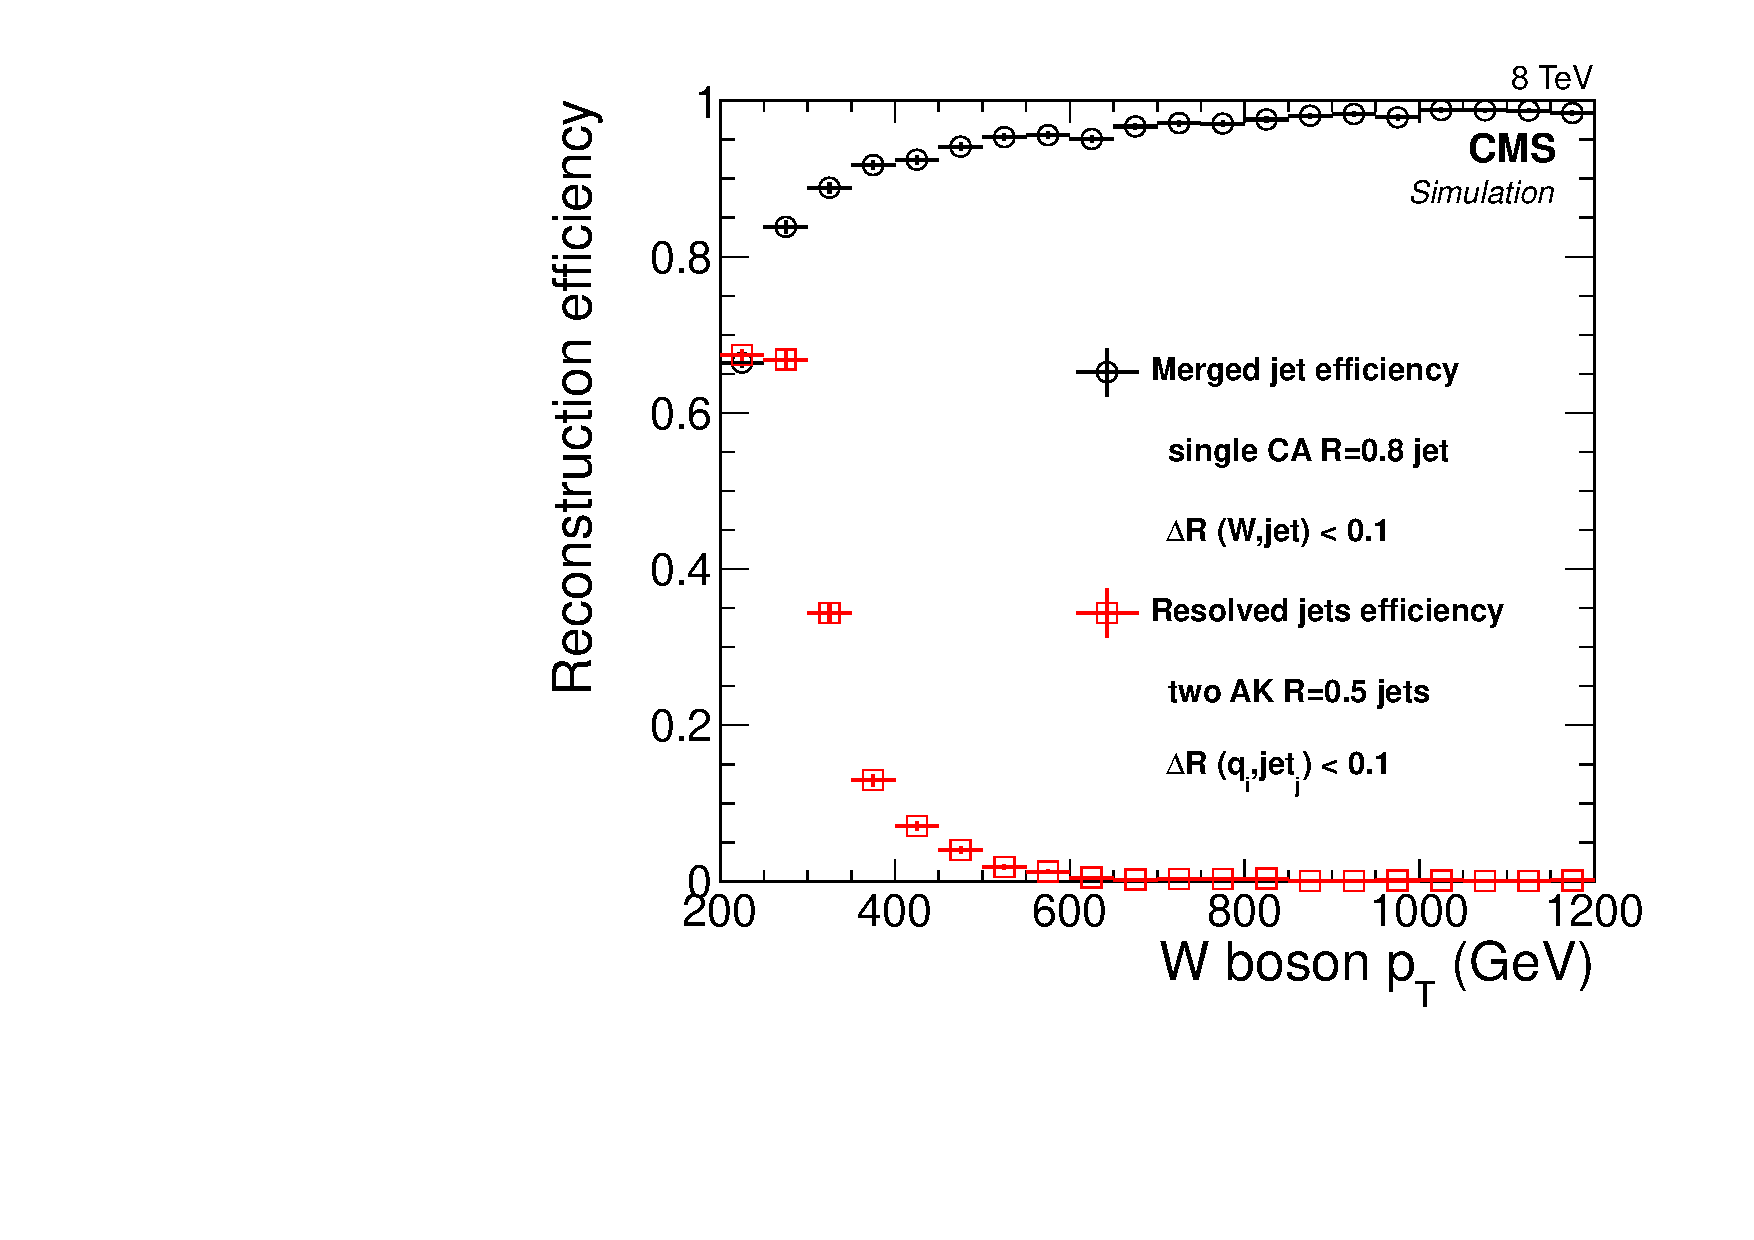
\includegraphics[width=0.45\textwidth]{\chsix/ca8effVsPt.pdf}
 \end{center}
 \caption{Efficiency to reconstruct a CA8 jet within $\Delta R <$ 0.1 of a generated W boson, and the efficiency to reconstruct two AK5 jets within $\Delta R <$ 0.1 of the generated quarks in the W-boson decay, as a function of the \pt of the W boson~\cite{Khachatryan:2014vla}.}
 \label{fig:ca8effVsPt}
\end{figure}

%%%%%%%% 
\subsection{Jet reconstruction and calibration}\label{subsec:jetsreco} %https://twiki.cern.ch/twiki/bin/view/CMSPublic/PhysicsResultsJME
%%%%%%%%

In CMS, the jet reconstruction is performed using the PF algorithm, which gives different reconstructed objects as input to the above-explained jet-clustering algorithms to build the so-called \textit{PF jets}.
%In CMS several standard methods for jet reconstruction are available which make use of different detector components, e.g. the tracker and the calorimeters, and give different reconstructed objects as input to the above explained jet clustering algorithms. In this work, only jets reconstructed with the PF algorithm are used and referred to as ``PF jets''.
%The so-called CaloJets are clustered from the energy measured in the electromagnetic and hadronic calorimeters (ECAL and HCAL) combined into towers. Jets can also be clustered from reconstructed charged particle tracks (TrackJets) or with the JetsPlusTracks (JPT) method [79] which combines reconstructed CaloJets with the information of the reconstructed tracks.
As sketched in Fig.~\ref{fig:PFalgo}, the PF algorithm aims at reconstructing all the stable particles produced in an event, combining the information coming from all CMS sub-detectors to optimize particle identification, direction and energy determination. These particles are classified in several types: charged hadrons, photons, neutral hadrons, electrons and muons. Jets are typically composed by 65\% charged hadrons, 25\% photons, 10\% neutral hadrons (Fig.~\ref{fig:PFjet_composition}). The PF algorithm is optimized to identify all these different components inside the jet, contrary to a calorimetric-only reconstruction. Typically, photons correspond to ECAL deposits not compatible with a tracker track. Charged hadrons correspond to HCAL and/or ECAL deposits matched to an inner track and not compatible with an electron, whereas neutral hadrons are identified as HCAL deposits not matched to any track.
%Particle trajectories measured in the tracker are extrapolated through the detector volume and are matched to the energy deposits in the calorimeters.
The momentum of neutral particles is obtained from the corresponding calorimeter energy deposits, calibrated for the non-linear response of the calorimeters.
For charged particles, the momentum is determined combining the track momentum measured by the tracker with high resolution and the corresponding calibrated calorimeter energy deposits.
%While the momentum of neutral particles is measured in the calorimeters, the momentum of charged particles is measured by the tracker with a better resolution.
Hence, both the position and energy measurements are greatly improved with respect to calorimeter jets as this algorithm makes use of the tracking detectors and high granularity of the ECAL which is much higher than that of the HCAL. Once all the PF candidates in the event are reconstructed, they are used as input to the jet-clustering algorithms described in the previous section and a PF jet is formed.
The jet momentum is determined as the vectorial sum of all PF candidates in the formed jet providing its ``raw'' estimate. 

\begin{figure}[!htb]
 \begin{center}
  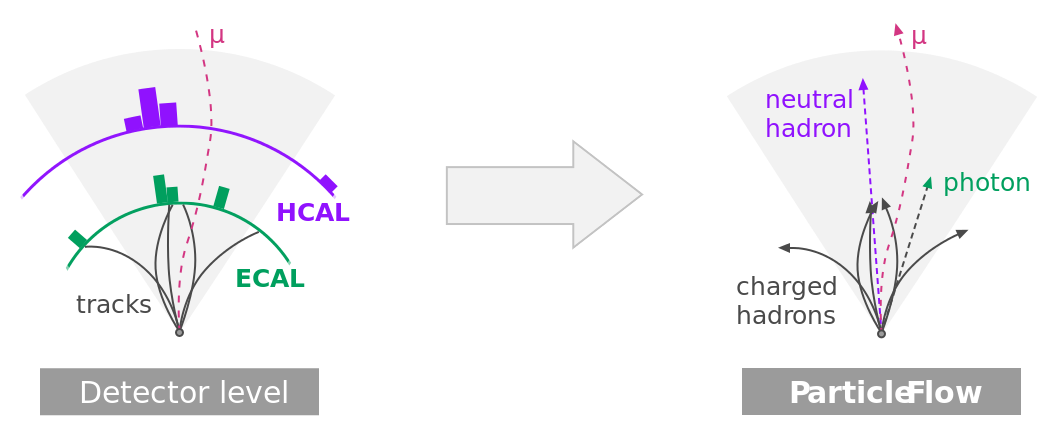
\includegraphics[width=0.7\textwidth]{\chsix/cms_particle_flow.png}
 \end{center}
 \caption{Sketch of the CMS particle-flow algorithm.}
 \label{fig:PFalgo}
\end{figure}

\begin{figure}[!htb]
\centering
\subfigure[]{\label{fig:PFjet_composition_a}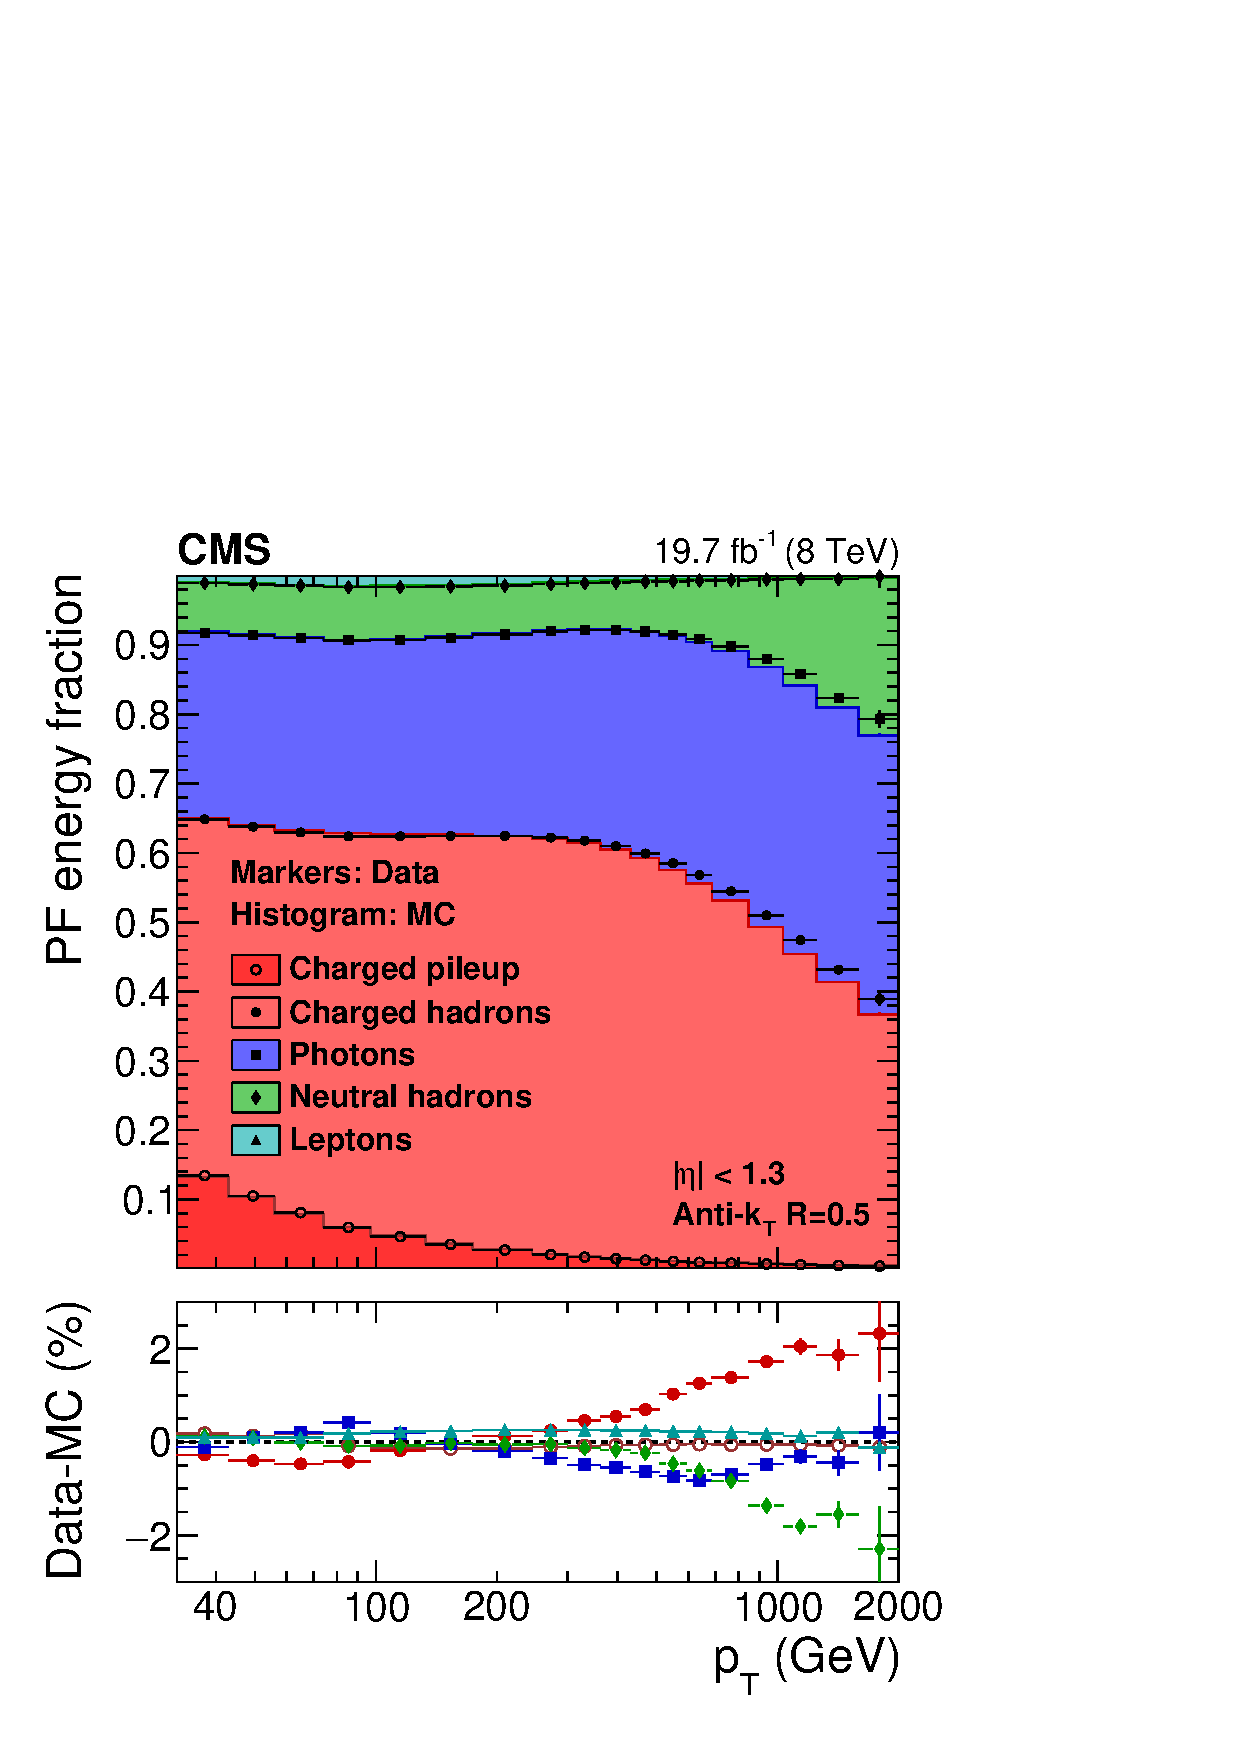
\includegraphics[width=0.45\textwidth]{\chsix/pfjet-composition-pt.pdf}}
\subfigure[]{\label{fig:PFjet_composition_b}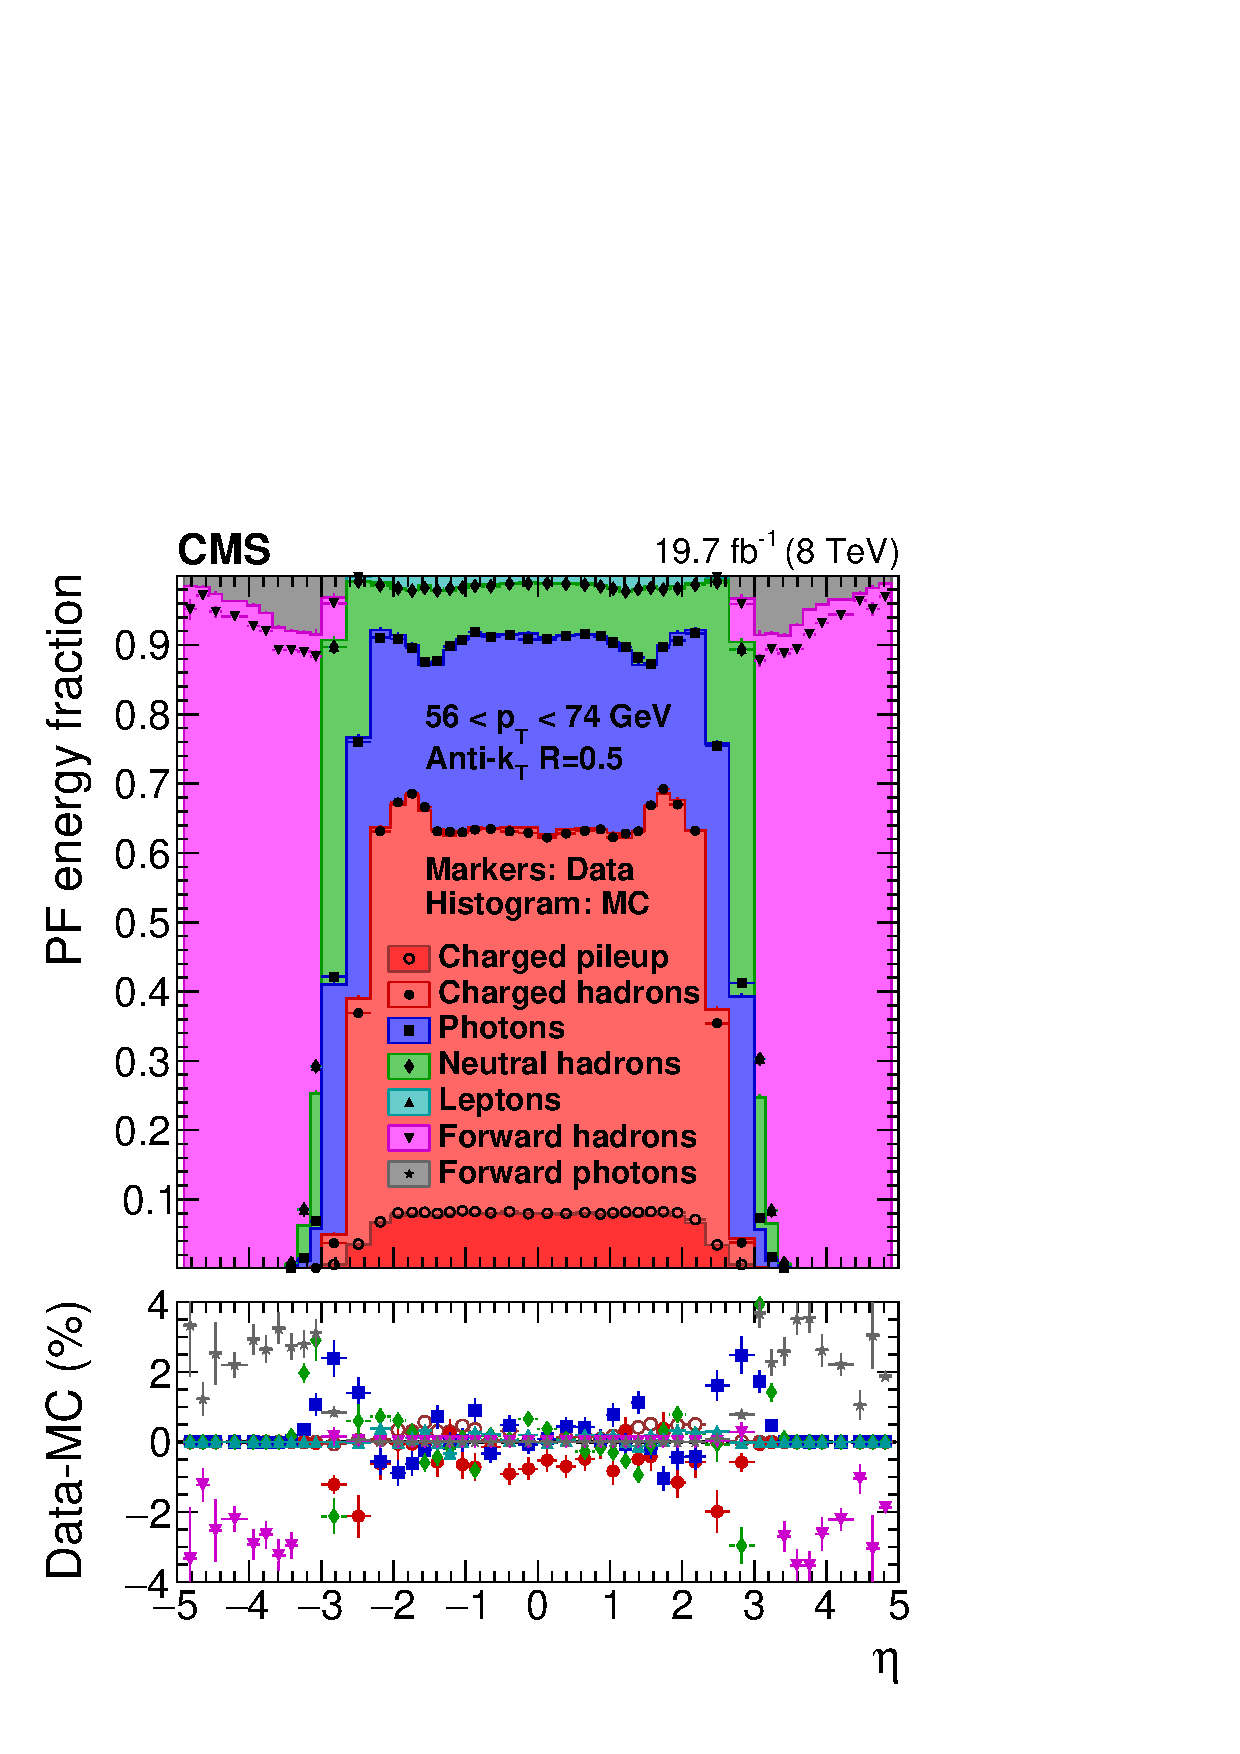
\includegraphics[width=0.45\textwidth]{\chsix/pfjet-composition-eta.pdf}}
\caption{PF jet composition in data and simulation as a function of jet \pt for jets with $|\eta| < 1.3$ (a), and as a function of $\eta$ for jets with \pt in the range $56 < \pt < 74\GeV$ (b)~\cite{Khachatryan:2016kdb}.}
\label{fig:PFjet_composition}
\end{figure}

The additional pp collisions occurring within the same bunch-crossing as the primary hard interaction produce additional tracks in the tracker and deposit energy in the calorimeters. This contribution is usually referred to as in-time pileup. Due to the finite signal decay time in the calorimeters, the pp collisions occurring in the previous and subsequent beam crossings also contribute to calorimetric energy in the same time window as the primary hard interaction. This contribution is called out-of-time pileup.
The out-of-time contribution is mitigated at the level of signal processing, while the in-time one is partially removed using tracking information. This is achieved by identifying which vertex the charged PF candidates originate from, and removing those unambiguously associated with pileup vertices before clustering jets. This method is referred to as \textit{charged-hadron subtraction} (CHS), and represents the reference standard method for jet reconstruction in CMS for Run~1 and beginning of Run~2.
%For the second part of Run~2, other pileup mitigation techniques in addition to CHS have been developed and tested in CMS~\cite{CMS-PAS-JME-13-005,CMS-PAS-JME-14-001,JME-16-003} but they are not used in this work. 

There are many possible sources of residual biases in the jet energy reconstruction, mainly due to the several intrinsic limitations of the system, such as the non-linear response of the calorimeters, the detector segmentation, the presence of material in front of calorimeters, electronic noise and pileup. The raw jet energy and resolution are thus corrected for several factors in order to obtain the energy value as close as possible to the true energy of the initial parton. CMS has adopted a factorized approach~\cite{1748-0221-6-11-P11002} to the problem of jet energy corrections, where each level of correction takes care of a different effect as described in the following.

The first step in this approach is a correction to the jet energies to mitigate additional pileup effects. 
In particular, the CHS jets are corrected to subtract residual contributions from neutral pileup particles, overlapping inside the jet cone. These corrections are determined from the simulation of a sample of QCD dijet events processed with and without pileup contaminations. This correction is usually parametrized as a function of the pileup energy density ($\rho$)~\cite{Cacciari:2011ma,Cacciari:2005hq}, the jet area (A)~\cite{Cacciari:2007fd}, jet \pt and $\eta$. The pileup offset corrections, defined as the mean value of the difference between the \pt of the reconstructed jet in events with and without pileup contamination, for AK5 CHS jets as a function of the corrected jet \pt and $\eta$ are shown in Fig.~\ref{fig:pucorr_ak5chs}, estimated for typical 2012 (8 TeV) conditions with an average number of additional pileup interactions $\left\langle\mu\right\rangle$ = 20.
The typical offset correction for a AK5 jet without CHS is 0.75 for a corrected jet \pt of 30\GeV, while a correction of 0.85 is obtained for AK5 CHS jets with same \pt value. This indicates that CHS removes approximately half of this offset before jet clustering by matching tracks to pileup vertices, reducing the residual offset correction. Roughly one third of the remaining pileup is from PF charged hadrons that have not been matched to good pileup vertices, and much of the rest is from PF photons. 

\begin{figure}[!htb]
\centering
\subfigure[]{\label{fig:pucorr_ak5chs_a}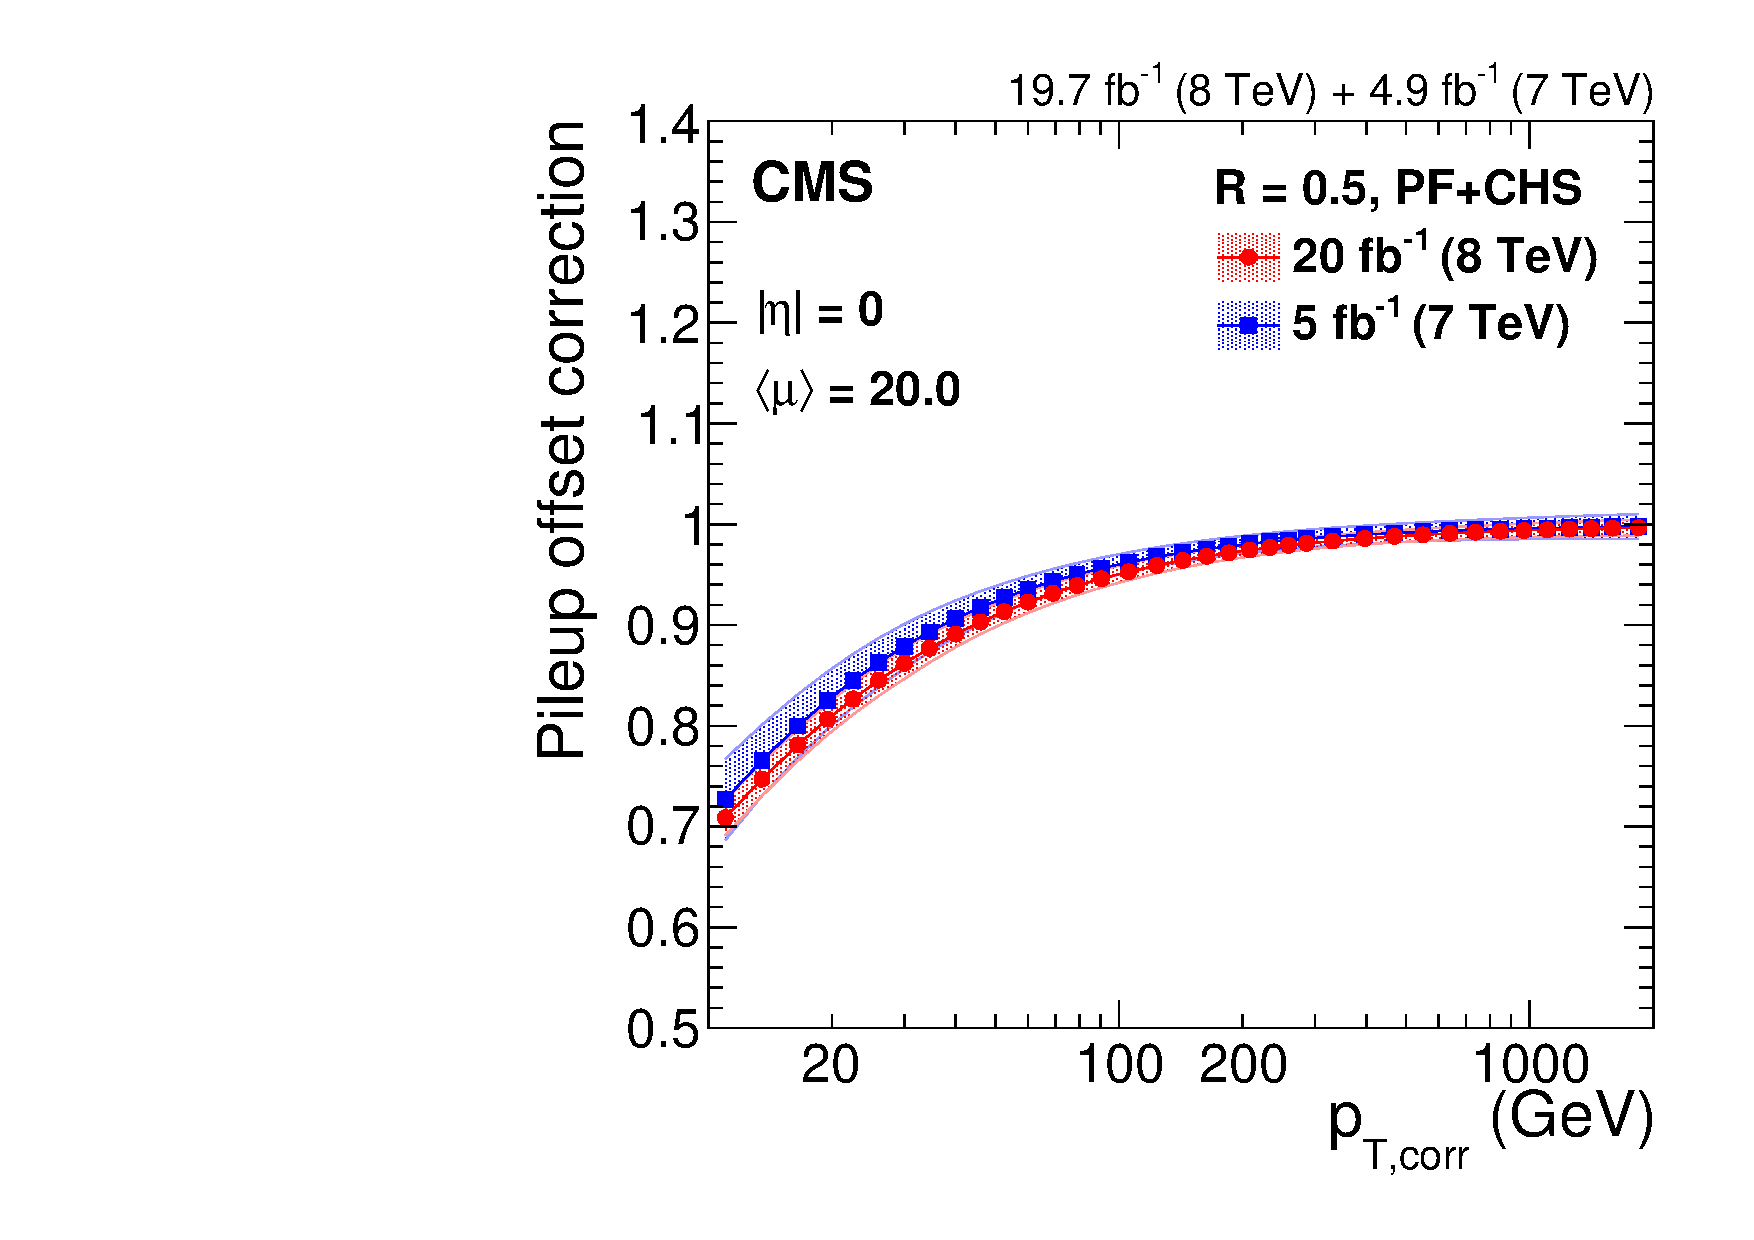
\includegraphics[width=0.45\textwidth]{\chsix/pu-corr-ak5chs-pt.pdf}}
\subfigure[]{\label{fig:pucorr_ak5chs_b}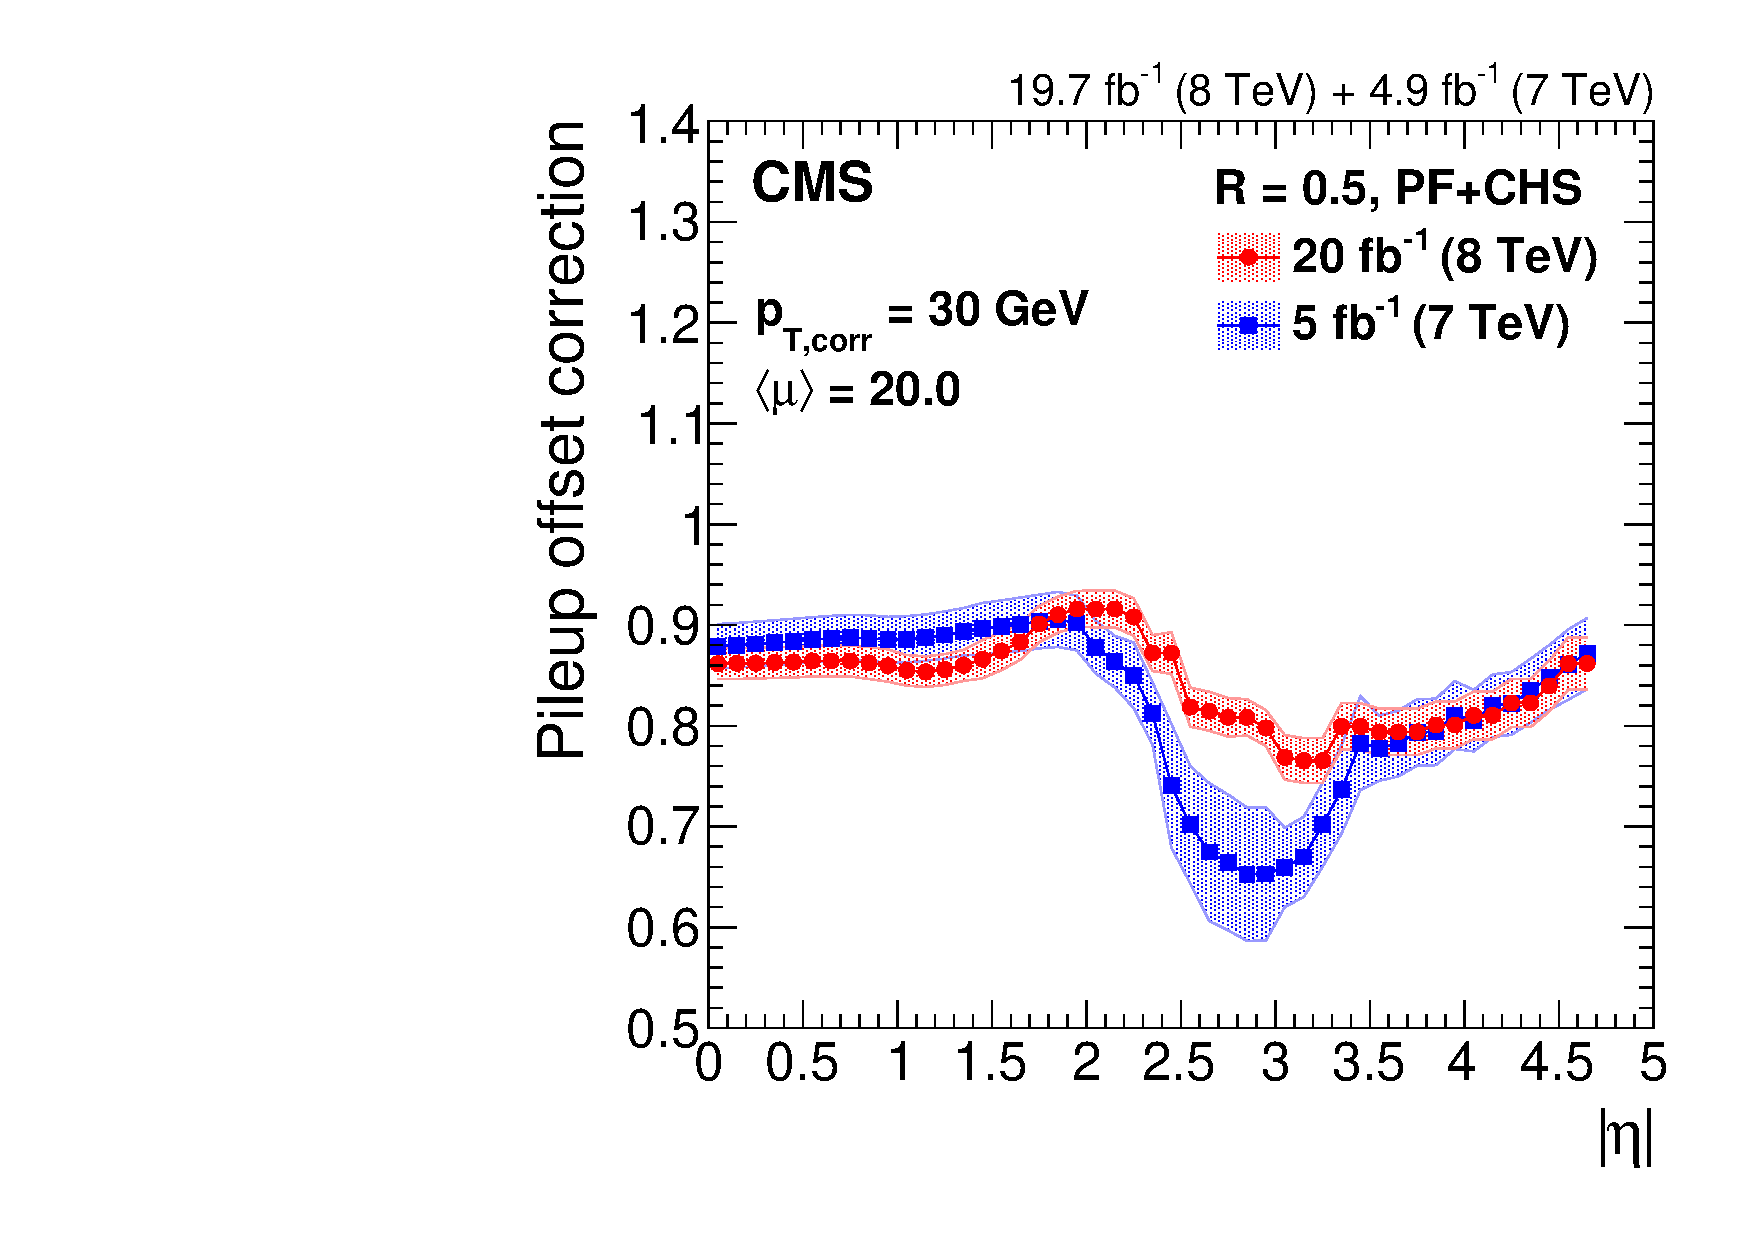
\includegraphics[width=0.45\textwidth]{\chsix/pu-corr-ak5chs-eta.pdf}}
\caption{Pileup offset correction for AK5 CHS jets estimated for the typical 2012 condition of $\left\langle\mu\right\rangle$ = 20. Corrections are shown for jets at $|\eta| = 0$ as a function of the corrected jet \pt (a), and for jets with $\pt = 30\GeV$ as a function of the jet $|\eta|$ (b)~\cite{Khachatryan:2016kdb}.}
\label{fig:pucorr_ak5chs}
\end{figure}

Secondly, a simulation-driven jet energy response correction is applied. The detector simulation takes into account effects due to
%particles deflected by the magnetic field,
energy lost when traversing the detector material, particle conversions, and a detailed detector geometry. In this step the aim is to correct for non-uniformities in the different CMS sub-detectors by comparing the reconstructed jet \pt to the particle-level one using simulated events only. The corrections are derived as a function of jet \pt and $\eta$ and make the response uniform over these two variables. The simulated particle response corrections are summarized in Fig.~\ref{fig:MCcorr_ak5chs} for 7 and 8\TeV data. The response is quite flat for $\pt > 50\GeV$, where the competing effects of increasing calorimeter response and falling tracking efficiency within the jet core compensate each other. In the barrel and endcap regions, the corrections rise with $|\eta|$, due to the increasing amount of material located in front of the calorimeters, which leads to effects such as an increased rate of nuclear interactions in the tracker. The corrections are higher around $|\eta|$ = 1.3 and 3.0 due to the degradation of the response in the transition regions.

\begin{figure}[!htb]
\centering
\subfigure[]{\label{fig:MCcorr_ak5chs_a}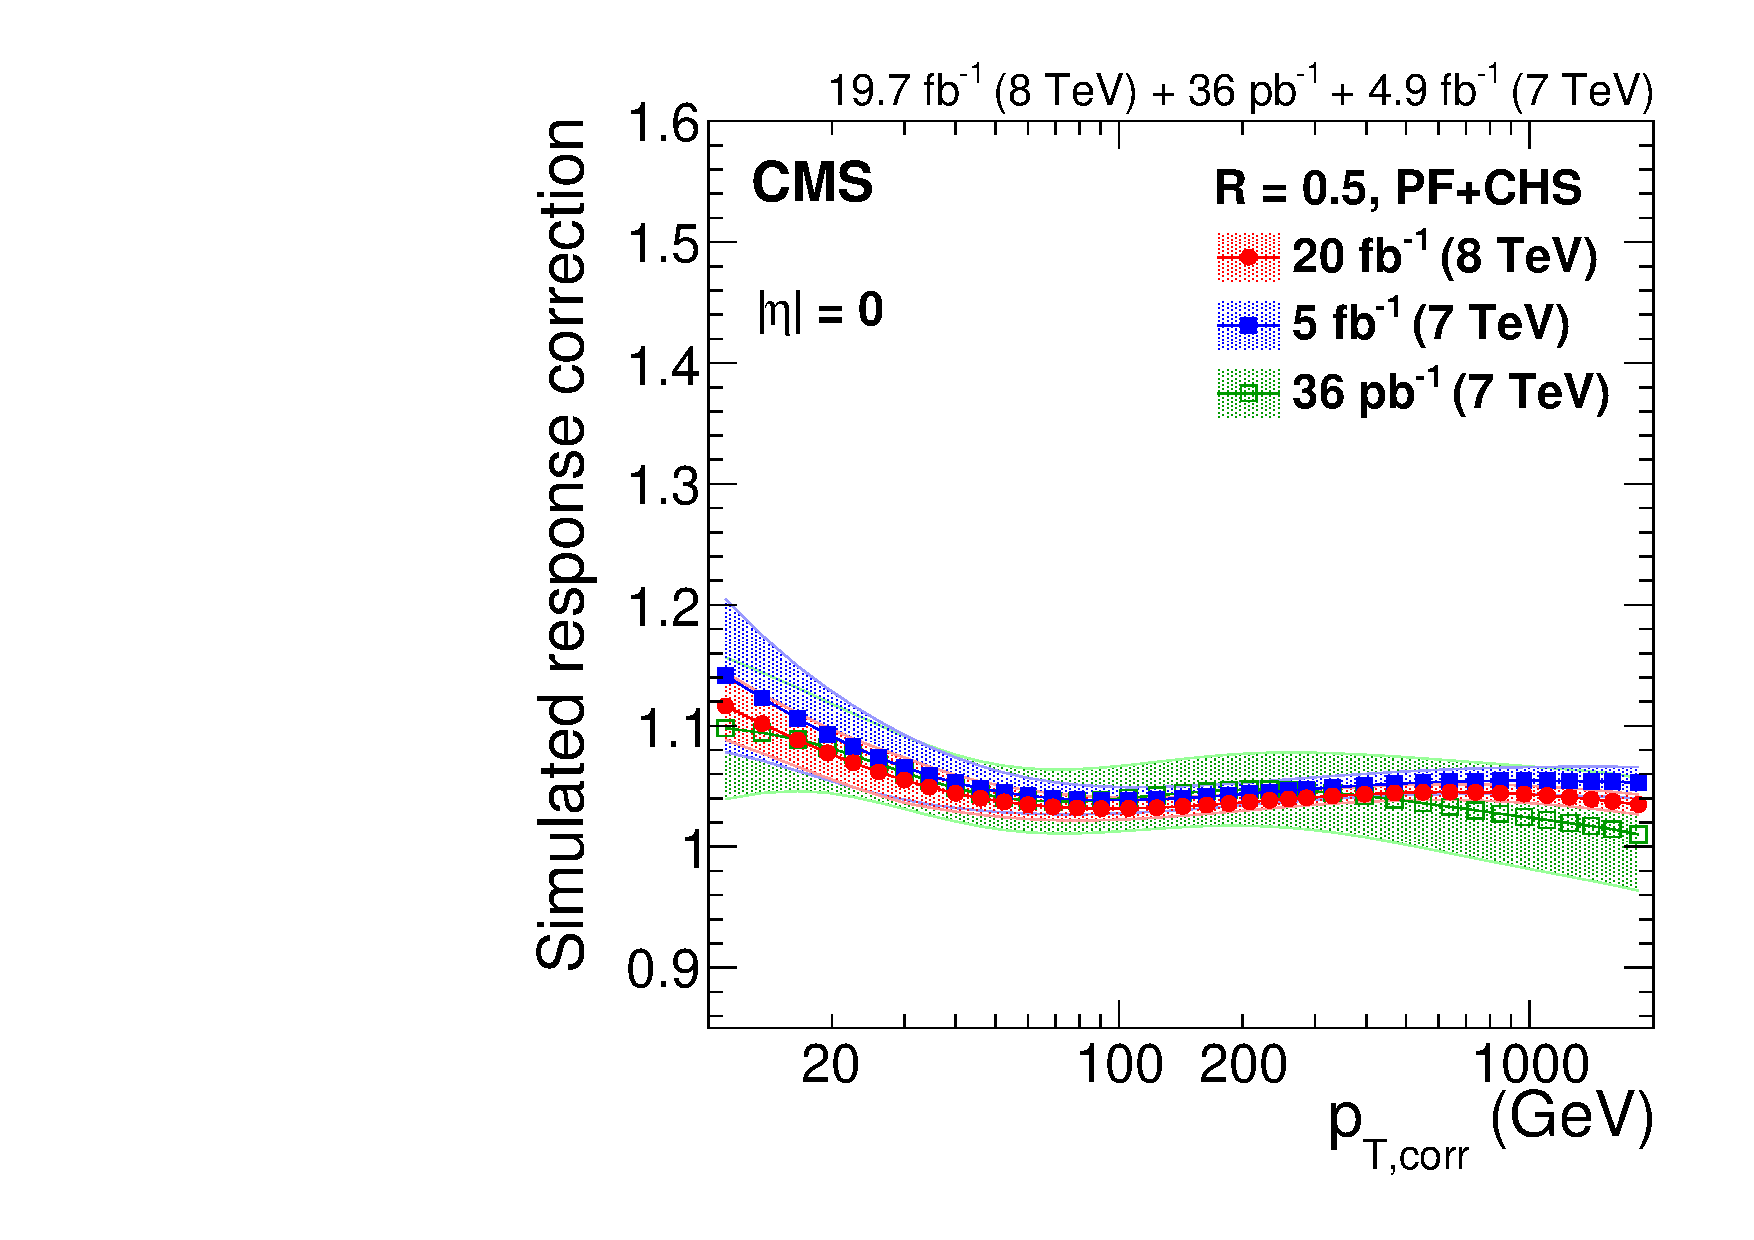
\includegraphics[width=0.45\textwidth]{\chsix/mc-corr-ak5chs-pt.pdf}}
\subfigure[]{\label{fig:MCcorr_ak5chs_b}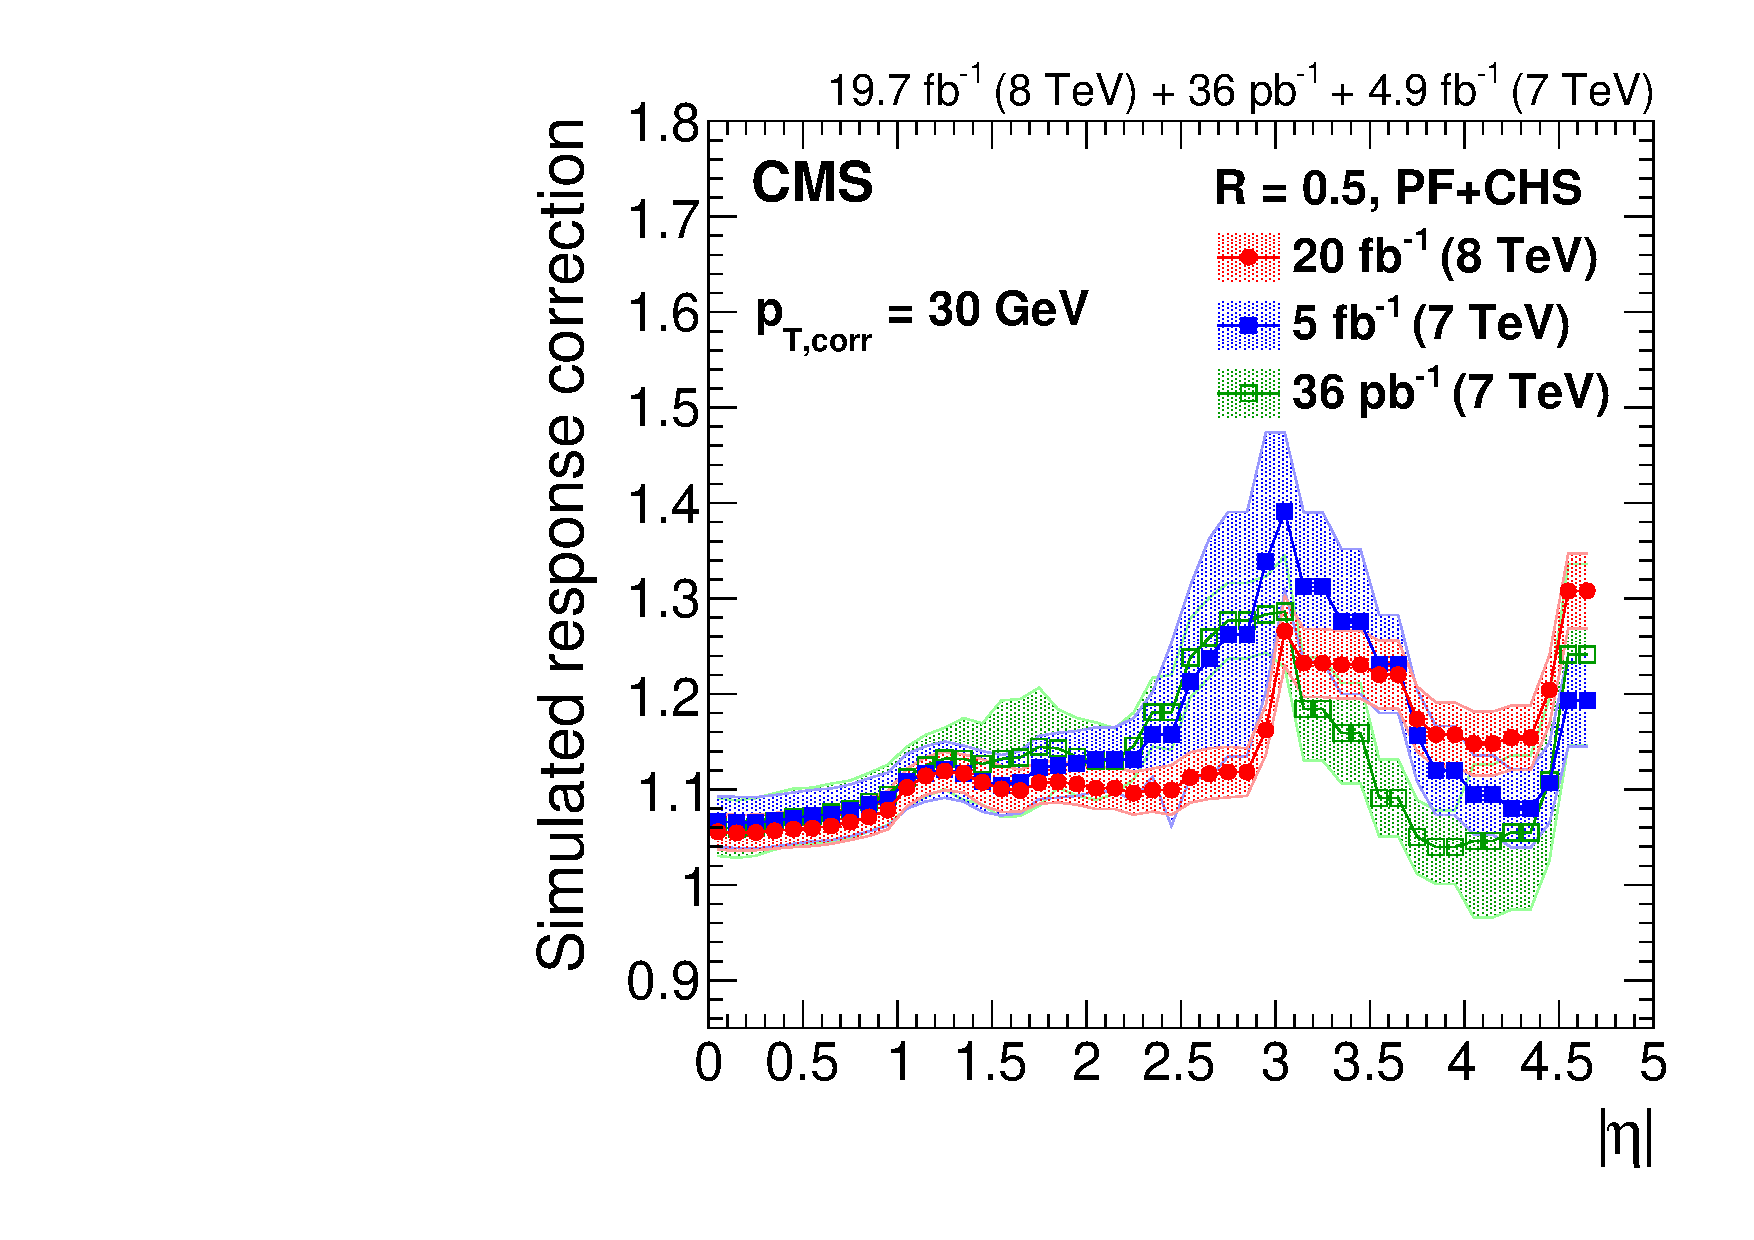
\includegraphics[width=0.45\textwidth]{\chsix/mc-corr-ak5chs-eta.pdf}}
\caption{Detector response correction factors for AK5 CHS jets estimated for the 8\TeV data collected in 2012. Corrections are shown for jets at $|\eta| = 0$ as a function of the corrected jet \pt (a), and for jets with $\pt = 30\GeV$ as a function of the jet $|\eta|$ (b)~\cite{Khachatryan:2016kdb}.}
\label{fig:MCcorr_ak5chs}
\end{figure}

Finally data-driven residual corrections are applied to correct for any measurable difference between the detector simulation and the jets measured in data. 
%This correction is done in two steps: first, the calibration as a function of jet $\eta$, and second, as a function of $\pt$.
This correction is done in two steps. At first, an additional correction for the non-homogeneous response of the detector with $\eta$ is derived from dijet events, in which the \pt response of a probe jet, outside the barrel region, is balanced with the one in the reference tag region ($|\eta| < 1.3$) as a function of the average \pt of the dijet system. Only events with back-to-back dijets and little additional activity in the event are used to avoid any impact from unbalanced events. %The result of the \pt-dependent fit is shown in Fig.~\ref{fig:rescorr_ak5chs_a}.
The jet energy is calibrated as a function of transverse momentum using a combination of Z($\to\ell\ell$)+jet, $\gamma$+jet, and multijet events for jets in the reference barrel region ($|\eta| < 1.3$). The basic idea, in all the considered topologies, is to exploit the transverse momentum balance between the jet to be calibrated and a well-reconstructed and calibrated reference object (Z or $\gamma$). The jet energy response is studied using two approaches. In one method the jet response is evaluated by comparing the reconstructed jet momentum ($p_\mathrm{T,jet}$) directly to the momentum of the reference object ($p_\mathrm{T,ref}$), while the second, more advanced, method takes into account the missing energy measured in the calorimeters to balance the reference object and jet momenta. In this method the additional event activity is taken into account by the missing energy. Therefore, additional jets in the event have only a small impact on the measurement. The residual corrections are summarized in Fig.~\ref{fig:rescorr_ak5chs} for 8\TeV data. The residual response corrections are less than 3\% in the barrel, less than 10\% in the endcaps, and about 10\% in the forward detector.

\begin{figure}[!htb]
\centering
\subfigure[]{\label{fig:rescorr_ak5chs_a}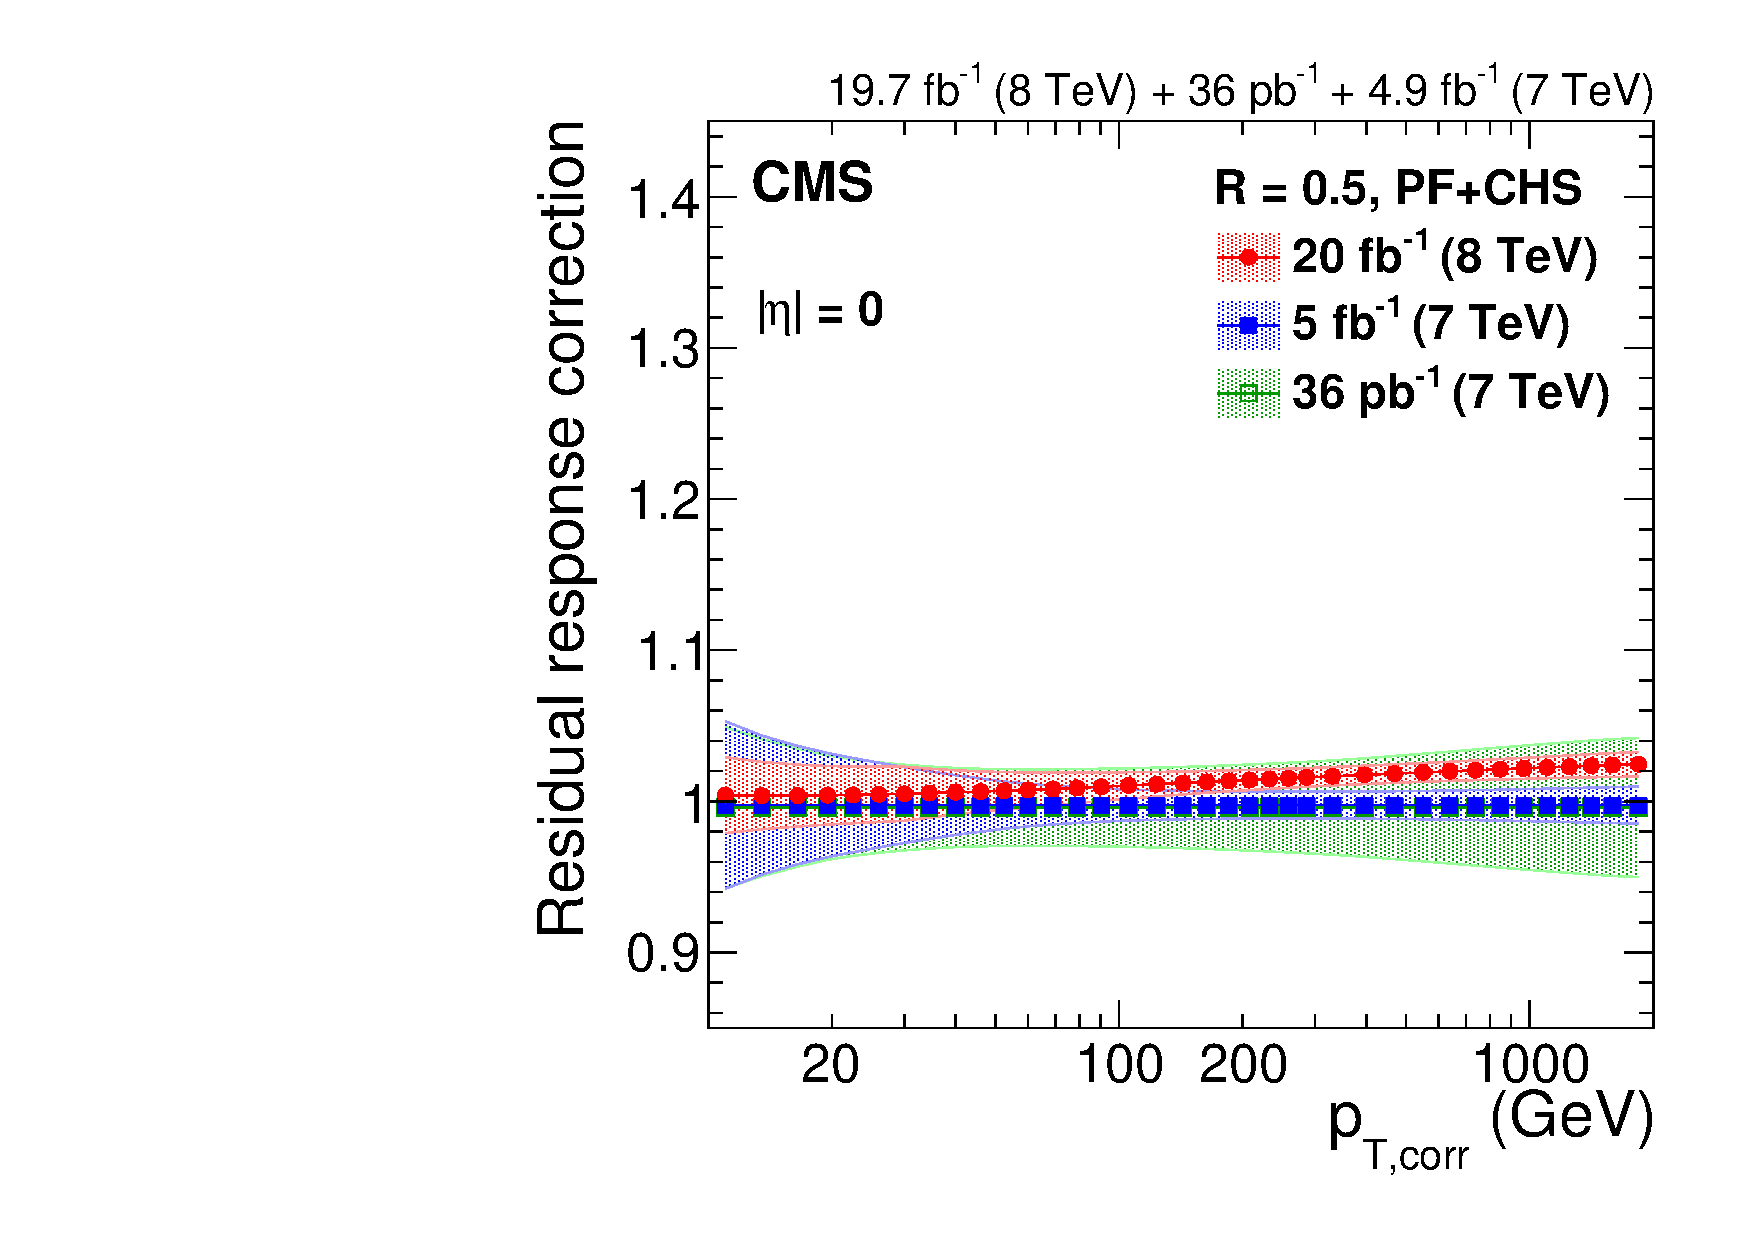
\includegraphics[width=0.45\textwidth]{\chsix/res-corr-ak5chs-pt.pdf}}
\subfigure[]{\label{fig:rescorr_ak5chs_b}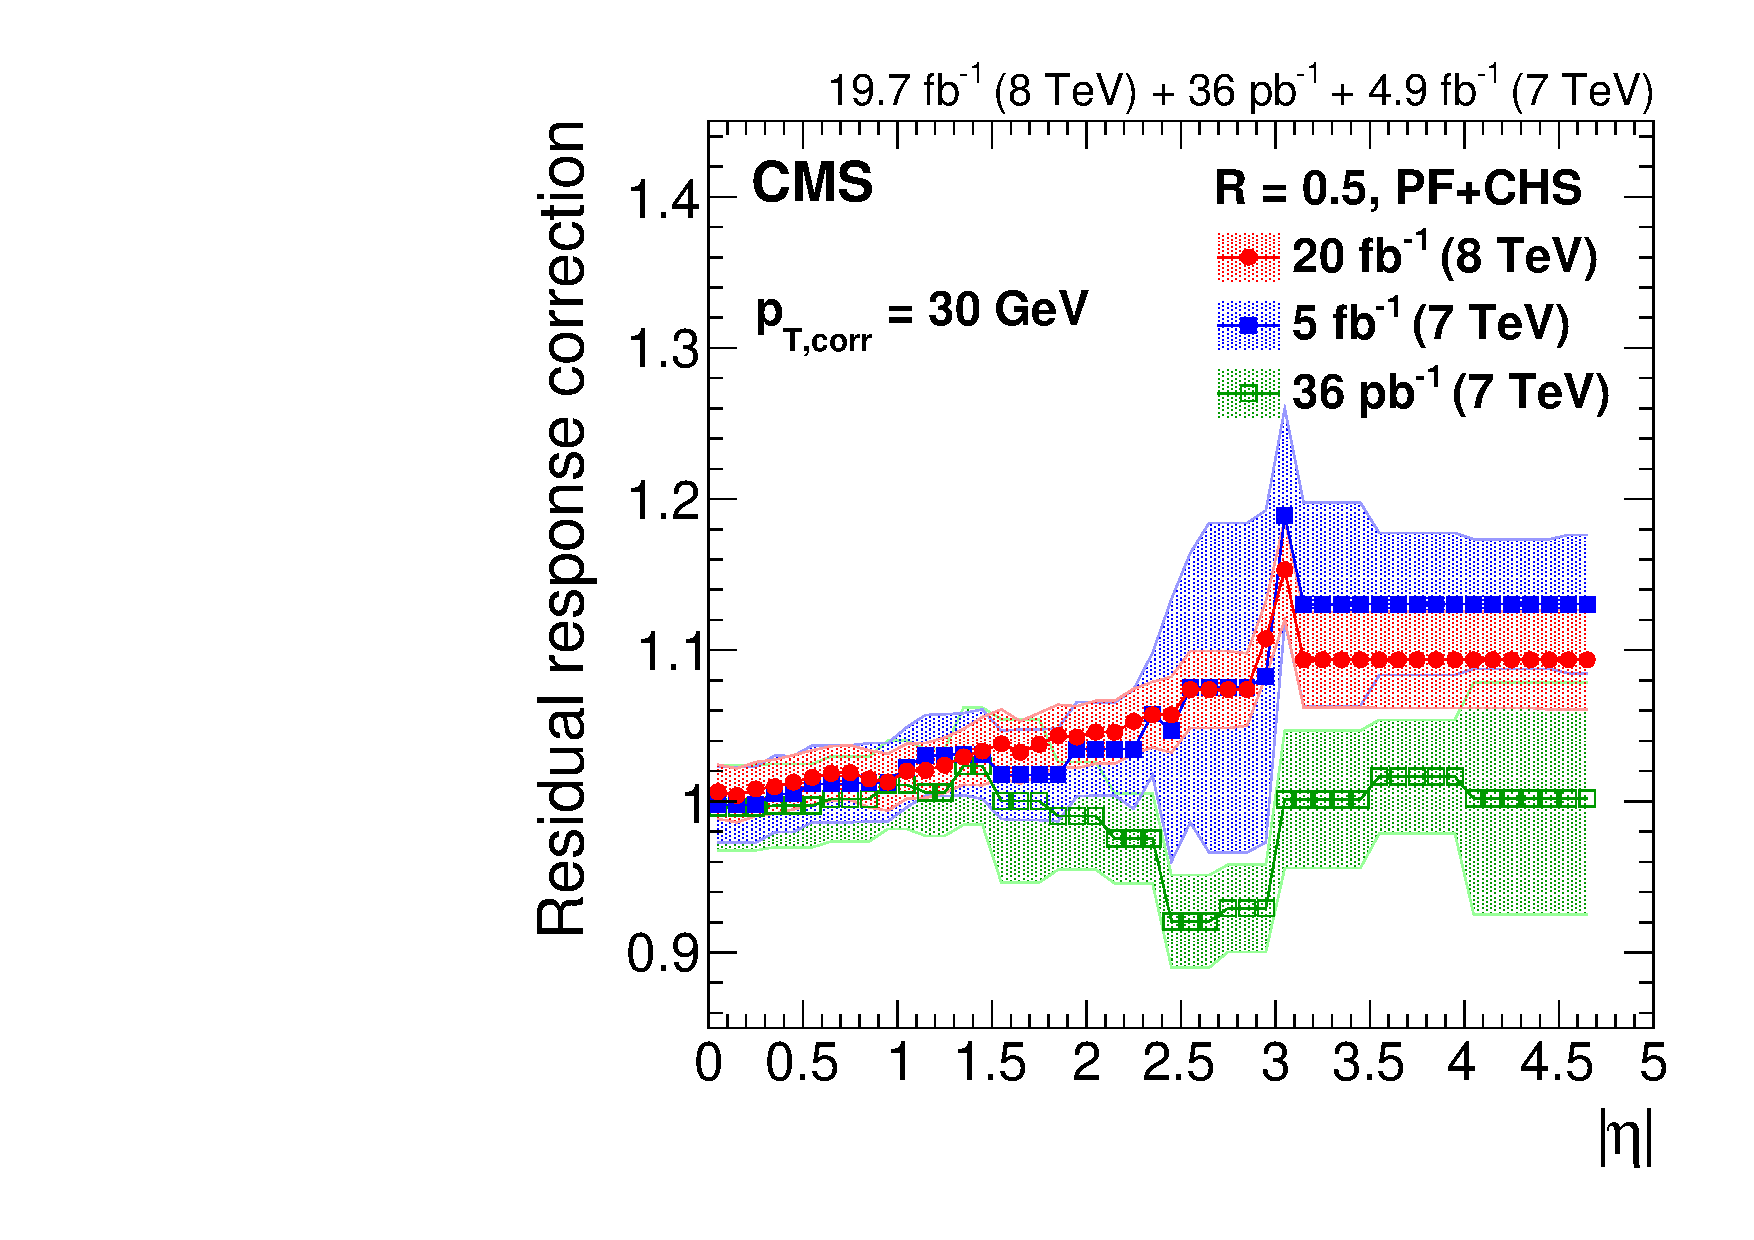
\includegraphics[width=0.45\textwidth]{\chsix/res-corr-ak5chs-eta.pdf}}
\caption{Residual data/simulation response correction factors for AK5 CHS jets for the 8\TeV data collected in 2012. Corrections are shown for jets at $|\eta| = 0$ as a function of the corrected jet \pt (a), and for jets with $\pt = 30\GeV$ as a function of the jet $|\eta|$ (b)~\cite{Khachatryan:2016kdb}.}
\label{fig:rescorr_ak5chs}
\end{figure}

The fully-calibrated PF jets are finally obtained in both data and simulation by multiplying all the above correction factors to the raw jet \pt as follows:

\begin{equation}
p_\mathrm{T,corr} = p_\mathrm{T,raw} \times C_\mathrm{pu}(p_\mathrm{T,raw},\eta,\rho\cdot\mathrm{A}) \times C_\mathrm{sim}(C_\mathrm{pu} \cdot p_\mathrm{T,raw},\eta) \times C_\mathrm{res}(C_\mathrm{pu} \cdot C_\mathrm{sim} \cdot p_\mathrm{T,raw},\eta)
\end{equation}

\noindent where $C_\mathrm{pu}$ represents the pileup correction, $C_\mathrm{sim}$ is the simulated response correction and $C_\mathrm{res}$ is the global residual correction applied only on jets in data.
Figure~\ref{fig:jesunc813TeV} shows the overall uncertainty on the corrections to the jet energy scale for AK5 and AK4 CHS jets for 8 and 13\TeV data, respectively. In both cases, the final uncertainties are below 3\% across the phase space of this analysis.

\begin{figure}[!htb]
\centering
\subfigure[]{\label{fig:jesunc_ak5chs_a}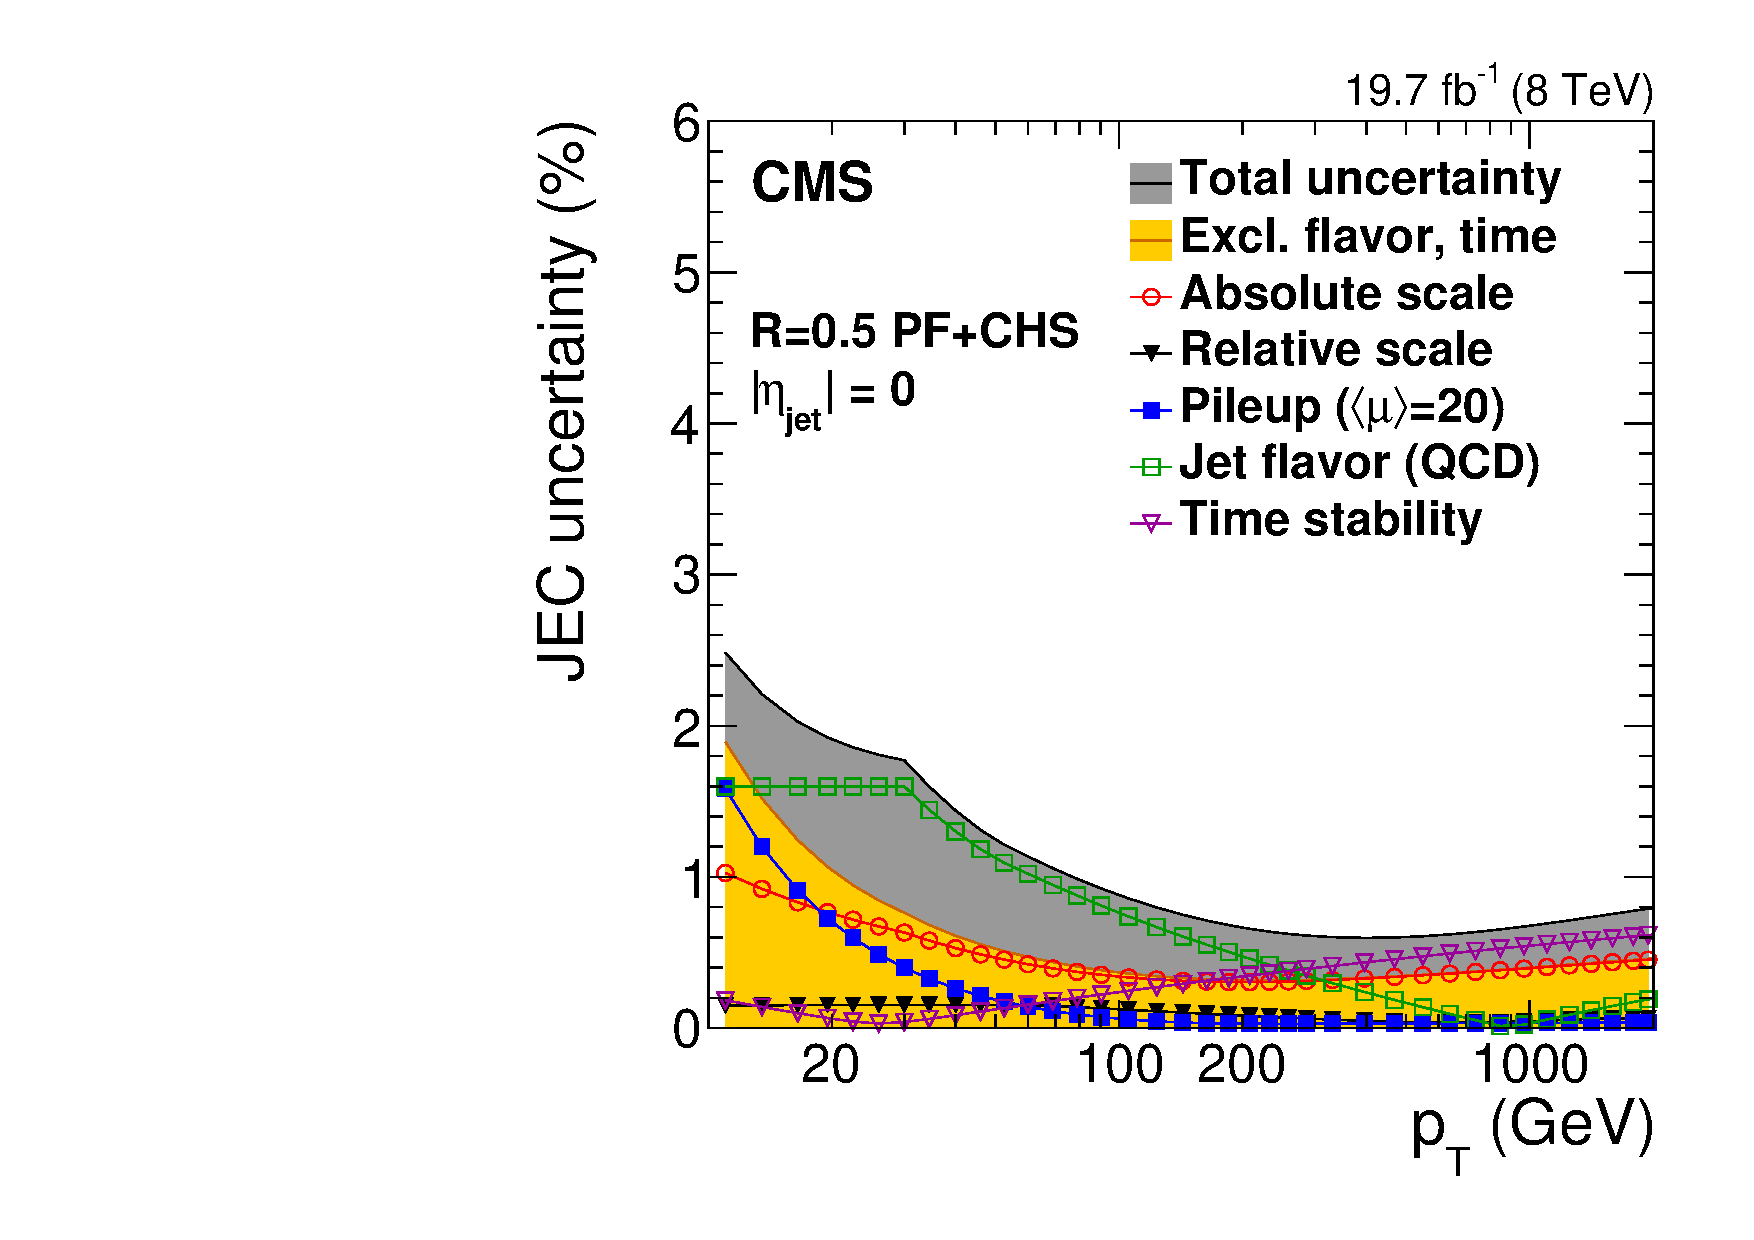
\includegraphics[width=0.45\textwidth]{\chsix/jesunc-ak5chs-pt.pdf}}
\subfigure[]{\label{fig:jesunc_ak5chs_b}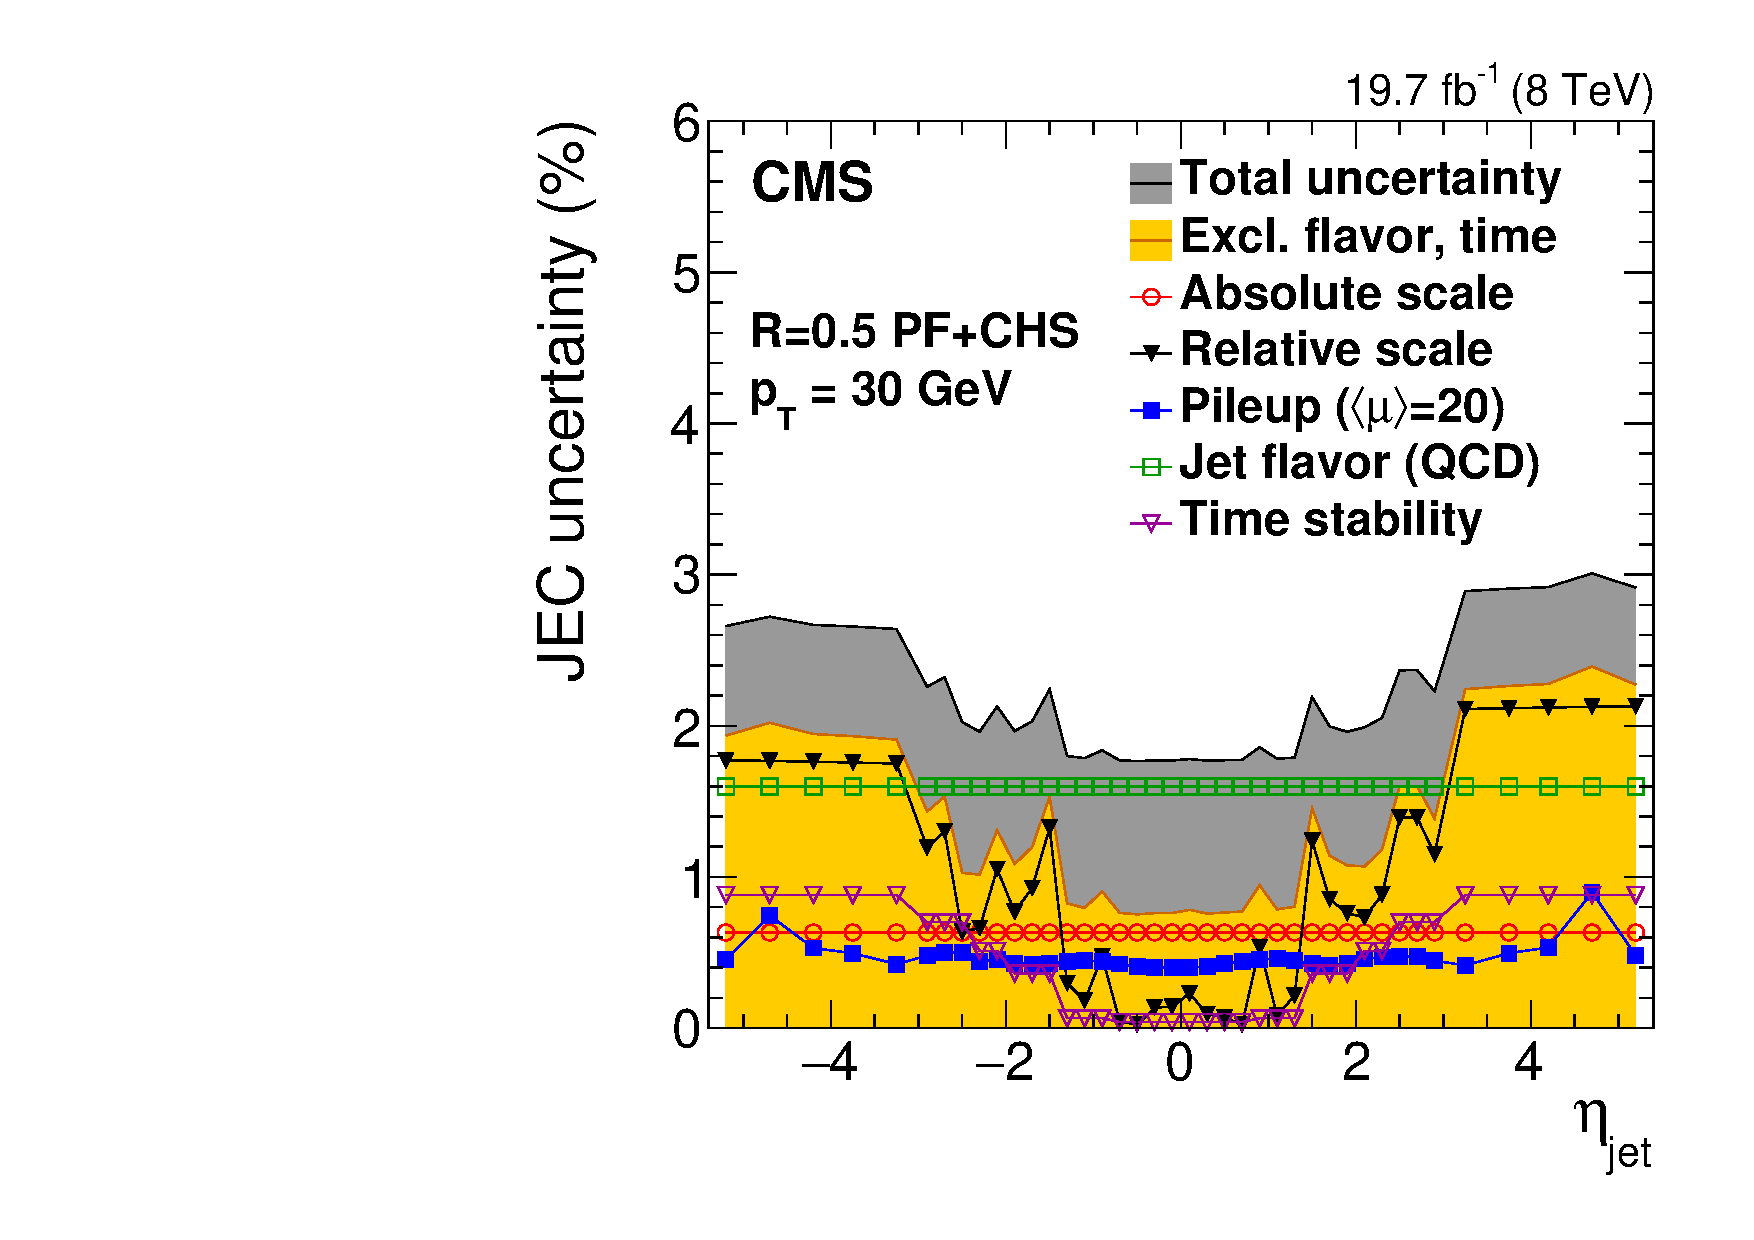
\includegraphics[width=0.45\textwidth]{\chsix/jesunc-ak5chs-eta.pdf}}\\
\subfigure[]{\label{fig:jesunc_ak4chs_c}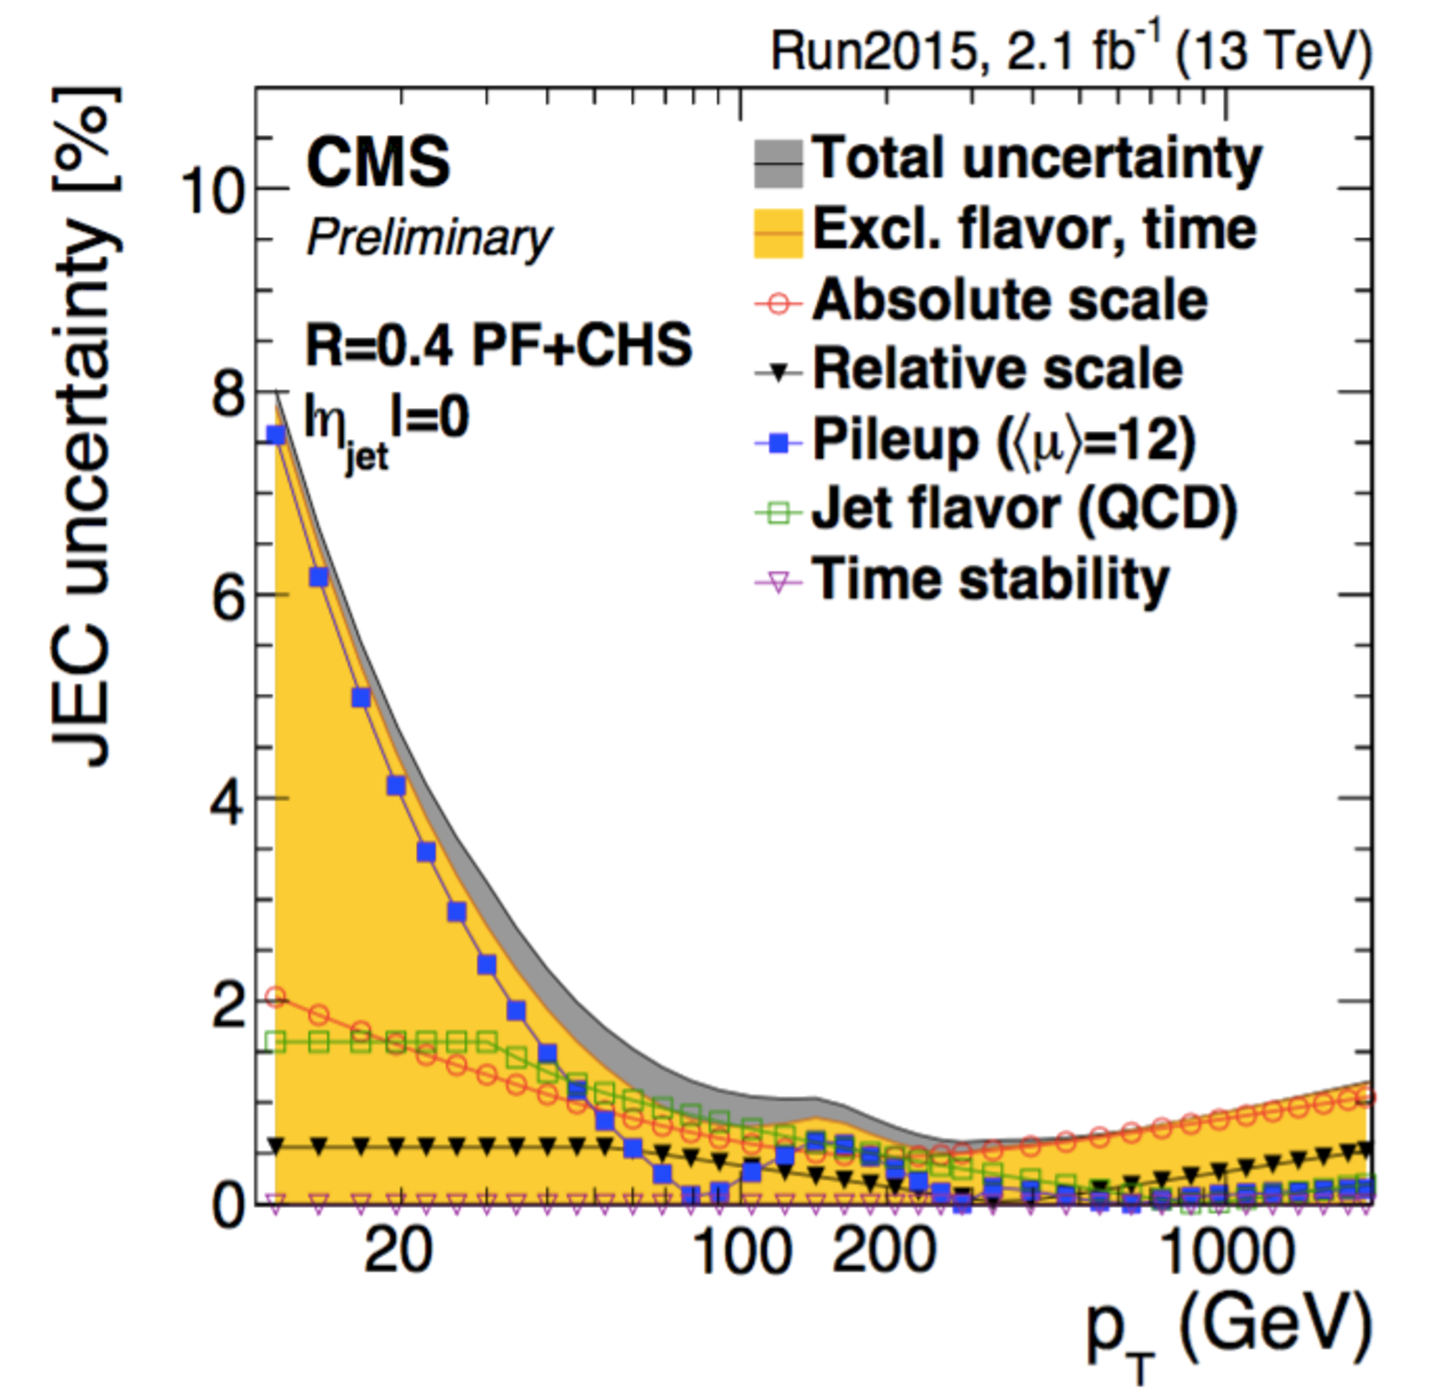
\includegraphics[width=0.45\textwidth]{\chsix/jesunc-ak4chs-pt.pdf}}
\subfigure[]{\label{fig:jesunc_ak4chs_d}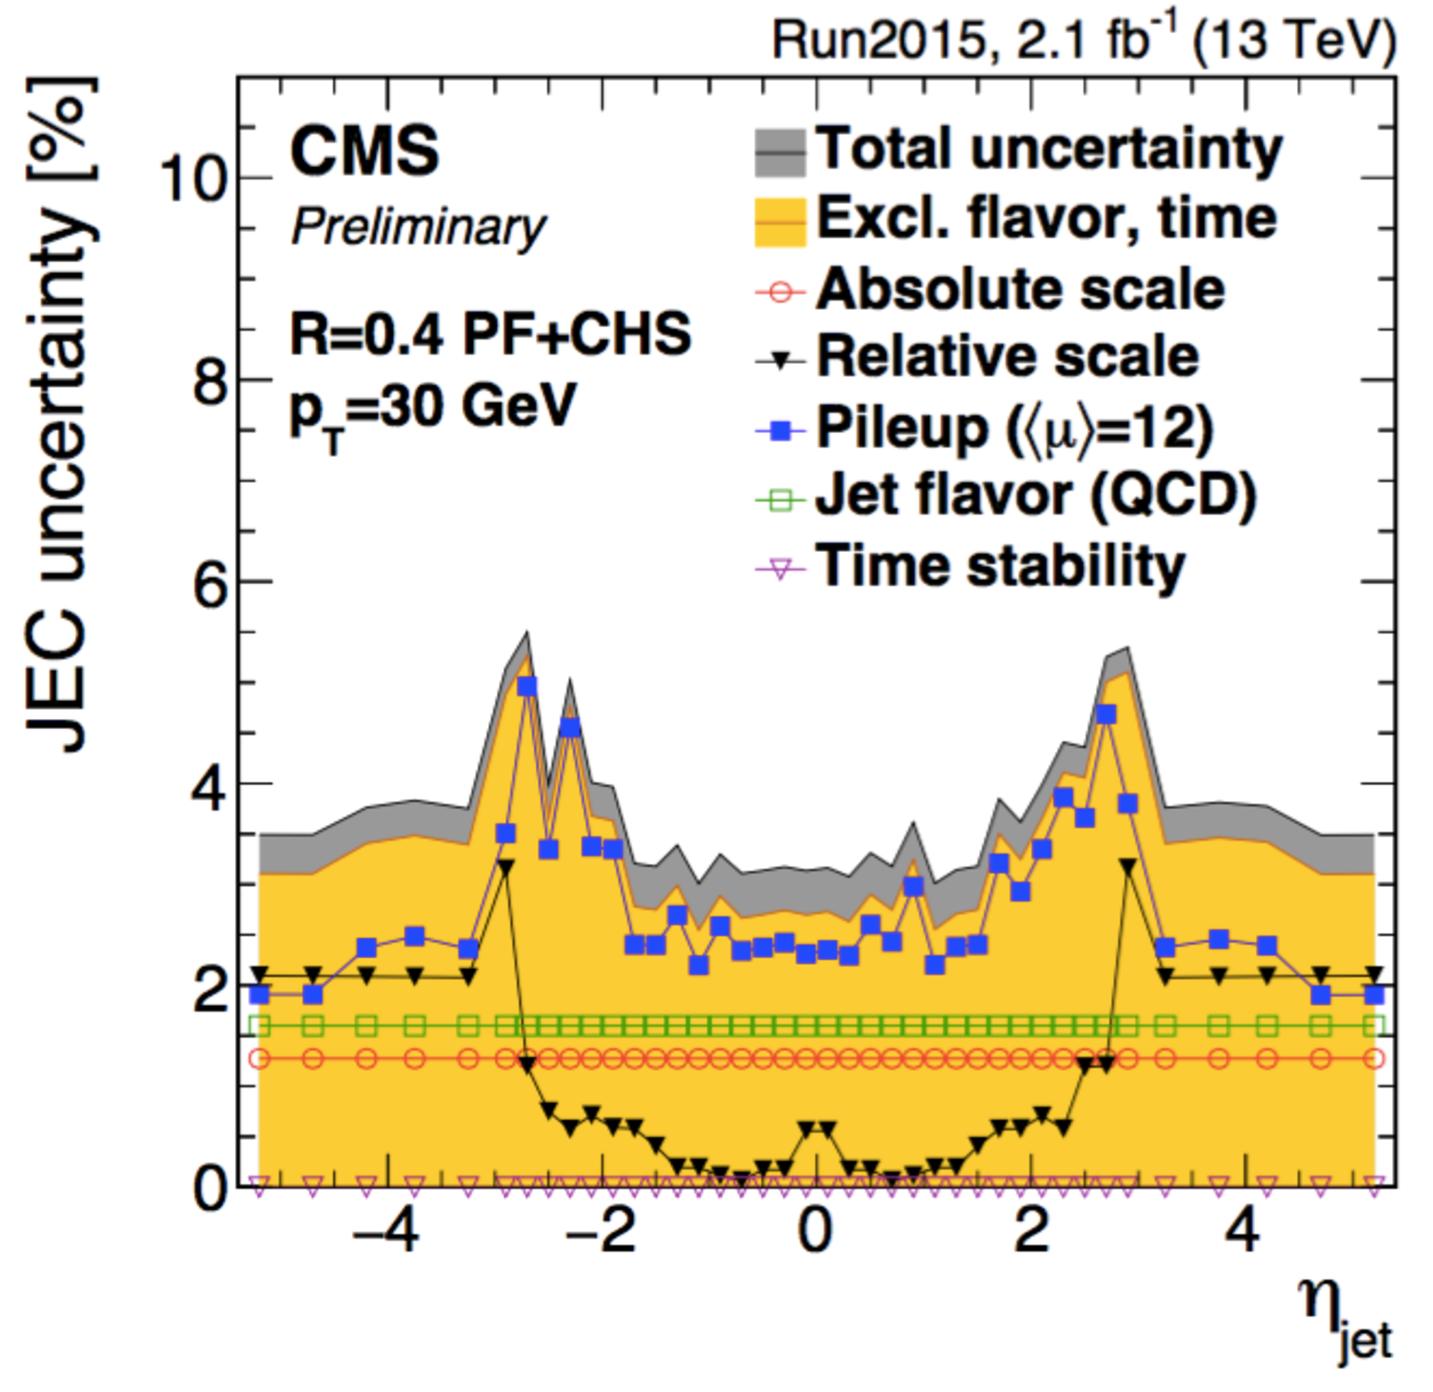
\includegraphics[width=0.45\textwidth]{\chsix/jesunc-ak4chs-eta.pdf}}
\caption{Summary of jet energy scale systematic uncertainties for the 8\TeV data collected in 2012 for AK5 CHS jets (upper plots) and for the 13\TeV data collected in 2015 for AK4 CHS jets (lower plots). Uncertainties are shown for jets at $|\eta| = 0$ as a function of the corrected jet \pt (left), and for jets with $\pt = 30\GeV$ as a function of the jet $|\eta|$ (right)~\cite{Khachatryan:2016kdb,CMS-DP-2016-020}.}
\label{fig:jesunc813TeV}
\end{figure}

The energy resolution of jets is relatively poor compared to the resolution of other physics objects (electrons, muons, photons), and the biases caused by jet resolution smearing are important for steeply falling spectra and for resonance decays. Hence, calibrations are evaluated to correct the jet energy resolution in addition to the corrections to the jet energy scale described above. The measurements are performed with methods which are extensions of the methods used for measuring jet energy scales, but instead of looking at the mean of the response distribution, the width is the interesting parameter. Furthermore, corrections have to compensate for effects that do not produce an overall shift in the mean, but that can widen the distribution. As shown in Fig.~\ref{fig:resolcorr813TeV}, the jet energy resolution in data is worse than in the simulation by 10--20\% depending on $\eta$, and the jets in simulation need to be smeared accordingly.\\
%Typical jet energy resolutions at the central rapidities are 15--20\% at 30\GeV, about 10\% at 100\GeV, and 5\% at 1\TeV. 
%The total uncertainty varies between 3--8\% for $|\eta| < 2.3$, increasing toward higher rapidity.

\begin{figure}[!htb]
\begin{center}
%\subfigure[]{\label{fig:resolcorr_ak5chs_a}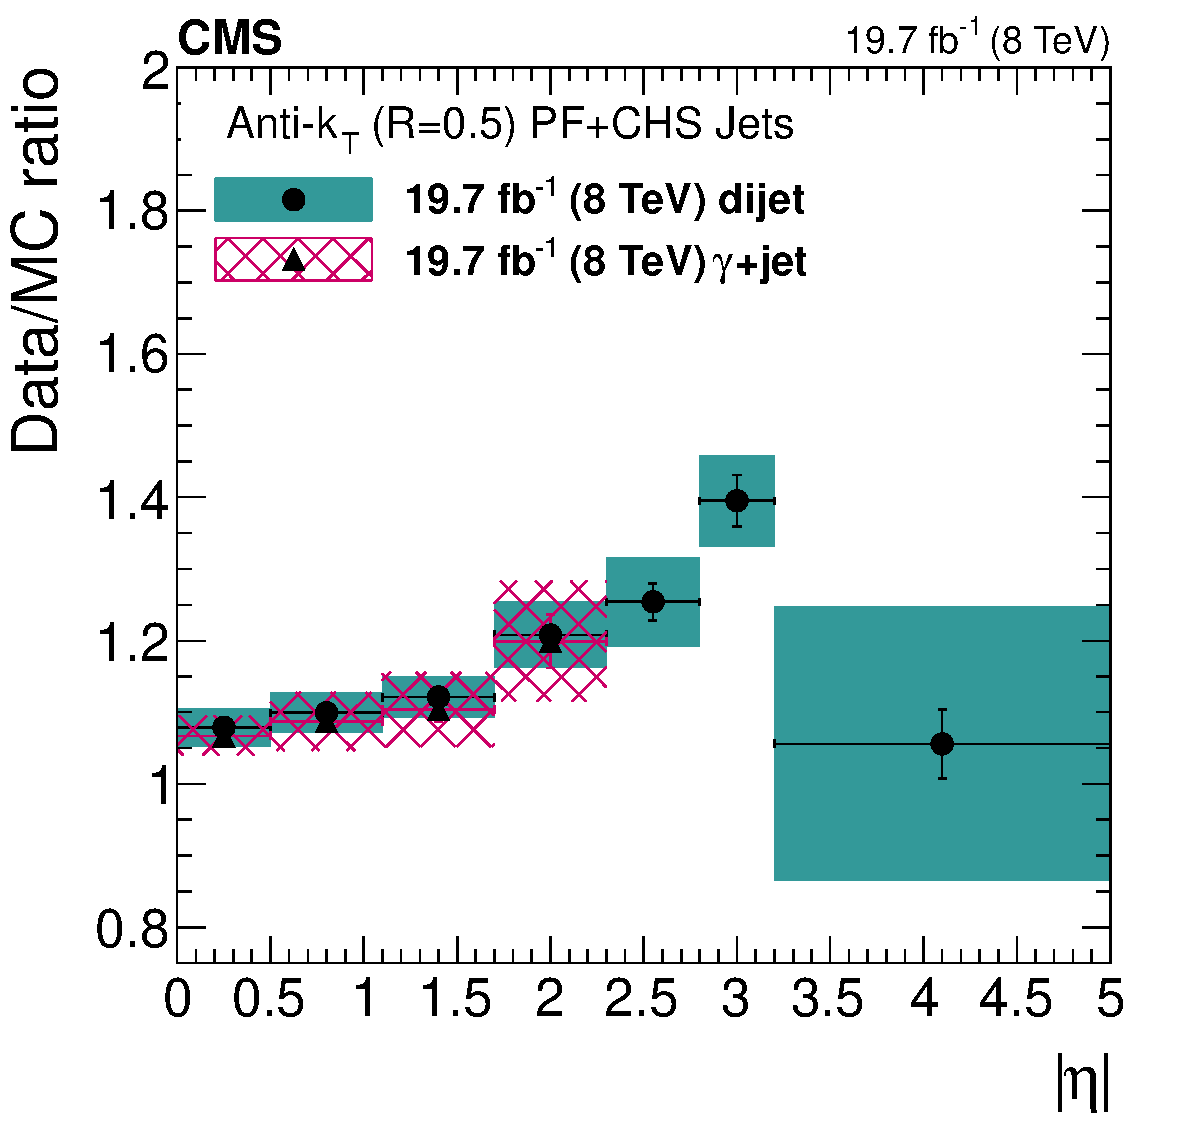
\includegraphics[width=0.45\textwidth]{\chsix/resolution-ak5chs-eta.pdf}}
%\subfigure[]{\label{fig:resolcorr_ak4chs_b}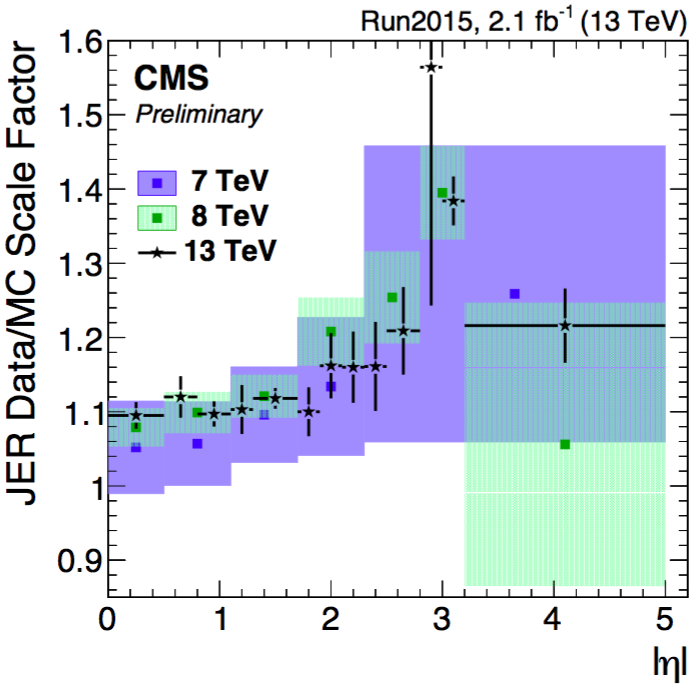
\includegraphics[width=0.45\textwidth]{\chsix/resolution-ak4chs-eta.png}}
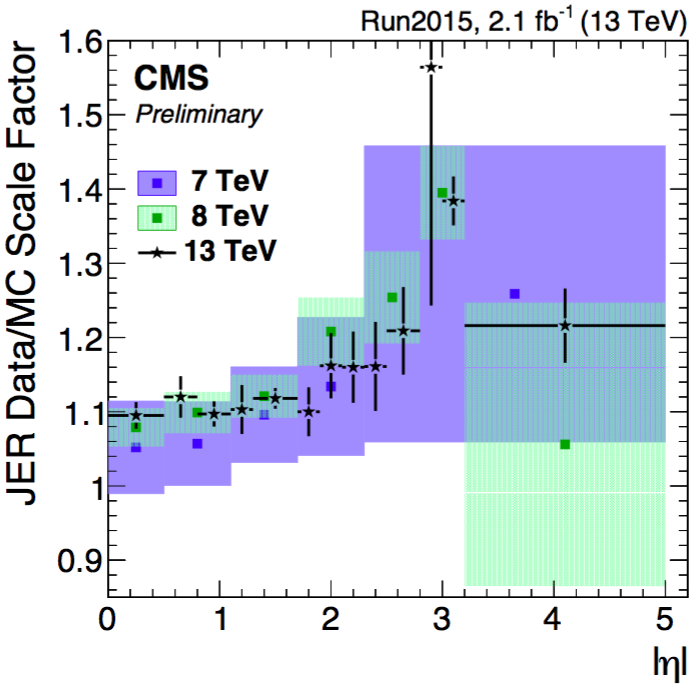
\includegraphics[width=0.45\textwidth]{\chsix/resolution-ak4chs-eta.png}
\end{center} 
\caption{Data-to-simulation scale factors for the jet \pt resolution for AK5 CHS jets as a function of $|\eta|$ determined from 8\TeV data collected in 2012, and for AK4 CHS jets in 13\TeV data collected in 2015~\cite{CMS-DP-2016-020}.}
\label{fig:resolcorr813TeV}
\end{figure}

Jets used in this analysis are requested to pass loose identification criteria, in order to reject spurious jet-like features originating from isolated noise patterns in the calorimeters or the tracker. The efficiency of these requirements is above 99\% for real jets~\cite{CMS-PAS-JME-10-003}. 

For the 8\TeV data analysis described in this work, all AK5 and CA8 jets must have corrected $\pt > 30\GeV$ and $> 200\GeV$, respectively, and $|\eta| < 2.4$ to be considered in the subsequent steps of the analysis.
Furthermore, the AK5 and CA8 jets are required to be separated from any well-identified muon or electron (Sections~\ref{sec:muons} and~\ref{sec:electrons}) by $\Delta R > 0.3$ and $> 0.8$, respectively. This requirement is applied to clean the jet collection used in the analysis from leptons clustered in jets. The AK5 jets are required to be separated from the CA8 jet representing the $\PV\to\qqbar$ candidate by $\Delta R > 0.8$ since an overlap is expected between the two reconstructions. Finally, CA8 jets are not used in the analysis if their pseudorapidity falls in the region $1.0 < |\eta| < 1.8$, thus overlapping the barrel-endcap transition region of the silicon tracker.
In fact, in Run~1 it has been found that in this region, `noise' can arise when the tracking algorithm reconstructs many fake displaced tracks associated with the jet.
This issue in the reconstruction has been studied in detail in the context of this work. The studies, presented and discussed in Appendix~\ref{app:tobtec}, resulted in the choice of the $\eta$ region to be excluded.
In particular, the simulation does not sufficiently describe the full material budget of the tracking detector in that region, thus it does not accurately describe this effect.
Without this requirement, a bias can be introduced in the b-tagging, jet-substructure and missing energy information, making this analysis systematically prone to that noise.
As a consequence of these results, other analyses involving similar kinematic cuts and identification algorithms have been affected~\cite{CMS-PAS-EXO-15-008}.
The same selections are applied for AK4 and AK8 jets in the 13\TeV data analysis, except for the fiducial cut on the $\eta$ of the large-cone jet since the aforementioned reconstruction issue has been fixed for Run~2.
%For the 13\TeV data analysis described in this work, all AK4 and AK8 jets must have corrected $\pt > 30\GeV$ and $> 200\GeV$, respectively, and $|\eta| < 2.4$ to be considered in the subsequent steps of the analysis.
%Furthermore, the AK4 and AK8 jets are required to be separated from any well-identified muon or electron (Sections~\ref{sec:muons} and~\ref{sec:electrons}) by $\Delta R > 0.3$ and $> 0.8$, respectively. This requirement is applied to clean the jet collection used in the analysis from leptons misidentified as jets. Finally, AK4 jets are required to be separated from the AK8 jet representing the $\PV\to\qqbarpr$ candidate by $\Delta R > 0.8$ since an overlap is expected between the two reconstructions. The same selections are applied for AK5 and CA8 jets in the 8\TeV data analysis. For this case an additional selection is applied to the pseudorapidity of CA8 jets.
%In particular, CA8 jets are not used in the analysis if their pseudorapidity falls in the region $1.0 < |\eta| < 1.8$, thus overlapping the barrel-endcap transition region of the silicon tracker.
%In fact, in Run~1 it has been found that in this region, `noise' can arise when the tracking algorithm reconstructs many fake displaced tracks associated with the jet.
%This issue in the reconstruction has been studied in details in the context of this work. The studies, presented and discussed in Appendix~\ref{app:tobtec}, resulted in the choice of the $\eta$ region to be excluded.
%In particular, the simulation does not sufficiently describe the full material budget of the tracking detector in that region, thus it does not accurately describe this effect.
%Without this requirement, a bias can be introduced in the b tagging, jet substructure and missing energy information, making this analysis systematically prone to that noise.
%As a consequence of these results, other analyses involving similar kinematic cuts and identification algorithms have been affected~\cite{CMS-PAS-EXO-15-008}.
%However, this problem has been fixed for Run~2 and this additional fiducial cut does not have to be applied in 13\TeV data analyses.

%%%%%%%% 
\subsection{Identification of b jets}\label{subsec:bjets}
%%%%%%%%
%https://twiki.cern.ch/twiki/bin/viewauth/CMS/BtagPOG
%https://twiki.cern.ch/twiki/bin/viewauth/CMS/BtagRecommendation
%https://twiki.cern.ch/twiki/bin/viewauth/CMS/BtagRecommendation74X
%https://twiki.cern.ch/twiki/bin/viewauth/CMS/BtagRecommendation53XReReco
%https://twiki.cern.ch/twiki/bin/view/CMSPublic/PhysicsResultsBTV

The identification of jets originating from b quarks (``b jets'') is one of the key ingredients of the analysis described in this work, which aims at isolating events of new physics with H bosons decaying to $\bbbar$. The ability to identify b jets (``b tagging'') plays a crucial role in reducing background coming from processes involving jets from gluons and light-flavor quarks (u, d, s), and from c-quark fragmentation.

Identifying b jets relies on the properties of the weak decay and fragmentation of the b hadrons formed from the original b quarks. The most important property is the relatively long lifetime of b hadrons of about 1.5\unit{ps} ($c\tau \equiv 450\mu m$) corresponding to a flight distance that is observable with high resolution tracking detectors. A b hadron with $\pt = 50\GeV$ propagates, on average, over almost half a centimetre ($L \sim \gamma c \tau$) before decaying. As shown in Fig.~\ref{fig:bjet}, this leads to secondary vertices displaced from the primary event vertex and charged particle tracks incompatible with the primary vertex with sizeable impact parameter. In addition, b hadrons have a large mass and large multiplicity of charged particles in the final state (about five charged particles on average per b-hadron decay). Because of the hard b-fragmentation function, the b hadron in a b jet carries a large fraction of the jet energy. Since b and c hadrons may decay semileptonically, in about 20\% (per lepton species) of the cases an electron or muon is produced inside a b jet, if both direct and cascade decays are taken into account.

\begin{figure}[!htb]
 \begin{center}
  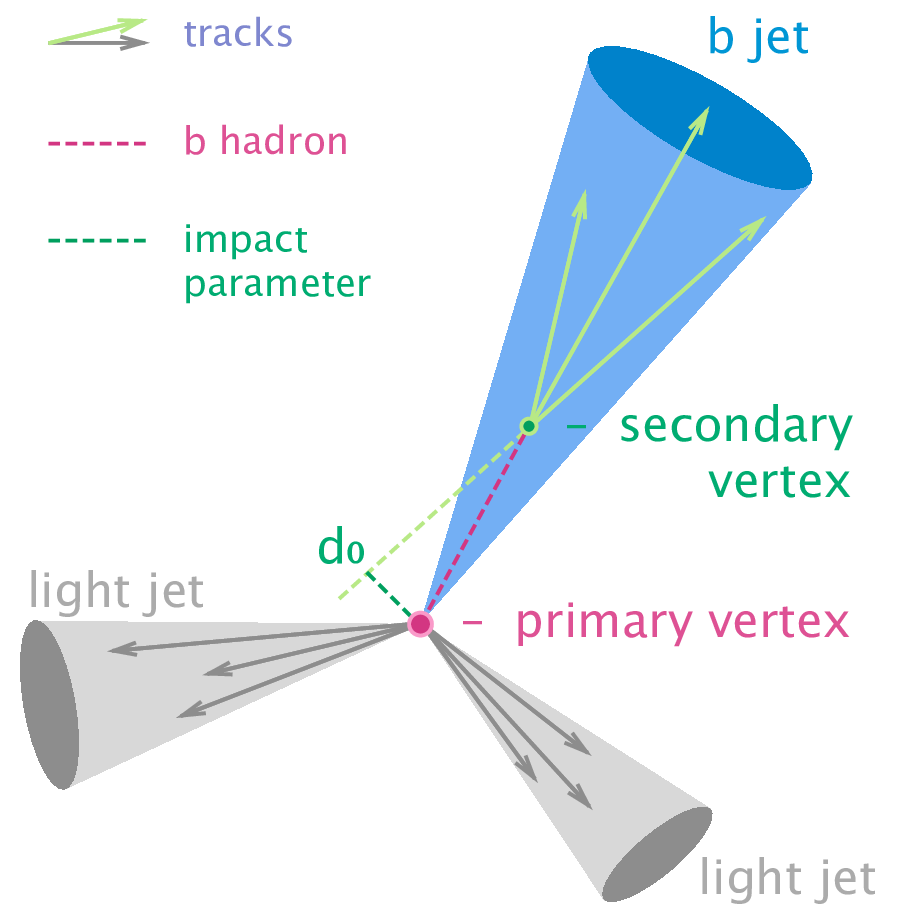
\includegraphics[width=0.5\textwidth]{\chsix/B-tagging_diagram.png}
 \end{center}
 \caption{Representation of a b-hadron decay and reconstructed b jet in the transverse plane.}
 \label{fig:bjet}
\end{figure}

A variety of algorithms have been developed in CMS~\cite{Chatrchyan:2012jua} that, starting from jets and charged tracks, identify b jets exploiting the b-hadron properties described above.
%These algorithms use low-level physics objects, mainly jets and charged tracks.
Only the tracking detectors offer the spatial resolution needed to measure the properties of b-hadron decays such as their long flight path. Efficient track reconstruction, and in particular precise spatial reconstruction close to the interaction point, is thus the key ingredient. 
Some of these algorithms use just a single observable, while others combine several of these objects to achieve a higher discrimination power. Each of these algorithms yields a single discriminator value for each jet. The minimum thresholds on these discriminators define loose (``L''), medium (``M''), and tight (``T'') operating points with a misidentification probability for light-flavor jets of 10\%, 1\%, and 0.1\%, respectively, at an average jet \pt of about 80\GeV.

The jets used for b tagging are reconstructed with the PF algorithm and calibrated as described in Section~\ref{subsec:jetsreco}. A sample of well-reconstructed tracks of high purity inside the jet is selected as input to each of the b-tagging methods. In addition to the selection applied in the iterative tracking procedure described in Section~\ref{subsec:tracks}, specific requirements are imposed on each track:

\begin{itemize}
\item $\pt >1\GeV, which reduces the  fraction of misreconstructed or poorly reconstructed tracks$;
\item at least 8 tracker hits (including pixel) must be associated with the track;
\item at least 2 hits are required in the pixel system since track measurements in the innermost layers provide most of the discriminating power;
\item the normalised $\chi^2$ is required to be $< 5$ to ensure a good-quality fit;
\item the absolute value of the transverse and longitudinal impact parameter of the track must be $< 0.2$ and $< 17\unit{cm}$, respectively, to reject charged particle tracks having their origin from sources with large displacement from the primary vertex (e.g. photon conversions and nuclear interactions in the beam pipe or the first layers of the pixel detector);
\item tracks must be associated to jets in a cone $\Delta R < 0.3$ around the jet axis, where the jet axis is defined by the primary vertex and the direction of the jet momentum;
\item the distance of closest approach of the track to the jet axis is required to be $< 700\mum$, in order to reject tracks from pileup;
\item the point of closest approach between the track trajectory and the jet axis, must be within 5\unit{cm} of the primary vertex.
\end{itemize}

Two algorithms for reconstructing secondary vertices are exploited. For the first algorithm, the tracks associated to jets and fulfilling the above selection requirements are used in the \textit{adaptive vertex reconstruction} (AVR) algorithm~\cite{Waltenberger:1166320}, based on the adaptive vertex fitter described in Section~\ref{subsec:tracks}. This is the secondary vertex reconstruction algorithm used for b-tagging methods in CMS during Run~1. A number of selection criteria are applied to remove vertices that are less likely to originate from a b-hadron decay. 

\begin{itemize}
\item at least 2 tracks must be associated to the secondary vertex;
\item the fraction of tracks shared with the primary vertex is required to be $< 65\%$;
\item the distance between the primary vertex and the secondary vertex in the transverse plane, the 2D flight distance, must be in the range 0.1--25\mm;
\item the 2D flight distance divided by its uncertainty or so-called 2D flight distance significance has to be $> 3$;
\item the invariant mass of charged particles associated to the vertex is required to be $< 6.5\GeV$ and not compatible with the mass of the $K^0_S$ hadron in a window of 50\MeV;
\item the angular distance $\Delta R$ between the jet axis and the secondary vertex flight direction is required to be less than the jet distance parameter;
\end{itemize}

In contrast to the AVR algorithm, the \textit{inclusive vertex finder} (IVF)~\cite{Khachatryan:2011wq} is not seeded from tracks associated to the reconstructed jets. The IVF algorithm uses as input the collection of reconstructed tracks in the event and looser quality criteria are applied. The selected tracks are then used to identify clusters of nearby tracks based on their minimum distance and the angles between them. The clusters are fit with the adaptive vertex fitter and a cleaning procedure is applied. At this stage, tracks can appear in multiple vertices and therefore, one of the vertices is removed based on the number of shared tracks and distance between the vertex and another one. Furthermore, tracks in the secondary vertex compatible with the primary vertex are removed. When there are at least 2 tracks associated to the secondary vertex after the track arbitration, the vertex is refit and selection criteria similar to the case of the AVR vertices are applied.

 The efficiency to reconstruct a secondary vertex for b (c) jets using the IVF algorithm is about 10\% (15\%) higher compared to the efficiency to reconstruct a secondary vertex with the AVR algorithm. However, for light-flavour jets the probability to find a secondary vertex also increases by about 8\%. Independently of the jet flavour, around 60\% of the jets with an AVR vertex also have an IVF vertex.\\
 
In this analysis the \textit{Combined Secondary Vertex} (CSV) b-tagging algorithm is used, which combines the information of displaced tracks with the information of secondary vertices associated to the jet.
%The CSV algorithm was further optimized and the new version is referred to as CSVv2 and it uses IVF.
This allows the algorithm to avoid limitations due to inefficiencies in the secondary vertex reconstruction. Jets are divided in three vertex-dependent exclusive categories: the presence of a reconstructed secondary vertex; at least two tracks with impact parameter significance larger than 2; none of the previous. The following set of variables with high discriminating power and low correlations are considered:

\begin{itemize}
\item the secondary vertex category;
\item the 2D flight distance significance of the secondary vertex;
\item the number of tracks in the jet;
\item the number of tracks associated to the secondary vertex;
\item the secondary vertex mass;
\item the ratio of the energy carried by tracks at the vertex with respect to all tracks in the jet;
\item the $\eta$ of the tracks at the vertex with respect to the jet axis;
\item the 2D impact-parameter significance of the first track that raises the invariant mass above the charm threshold of 1.5\GeV when subsequently summing up tracks ordered by decreasing impact parameter significance;
\item the 3D signed impact-parameter significance for each track in the jet.
\end{itemize}

Two likelihood ratios are built from these variables used to discriminate between b and c jets and between b and light-flavor jets and combined with prior weights of 0.25 and 0.75, respectively. Figure~\ref{fig:csv_813TeV_a} shows the distribution of the CSV discriminator value in a multijet sample for 8\TeV data and for simulation, for jets clustered with the AK5 algorithm.

\begin{figure}[!htb]
\begin{center}
\subfigure[]{\label{fig:csv_813TeV_a}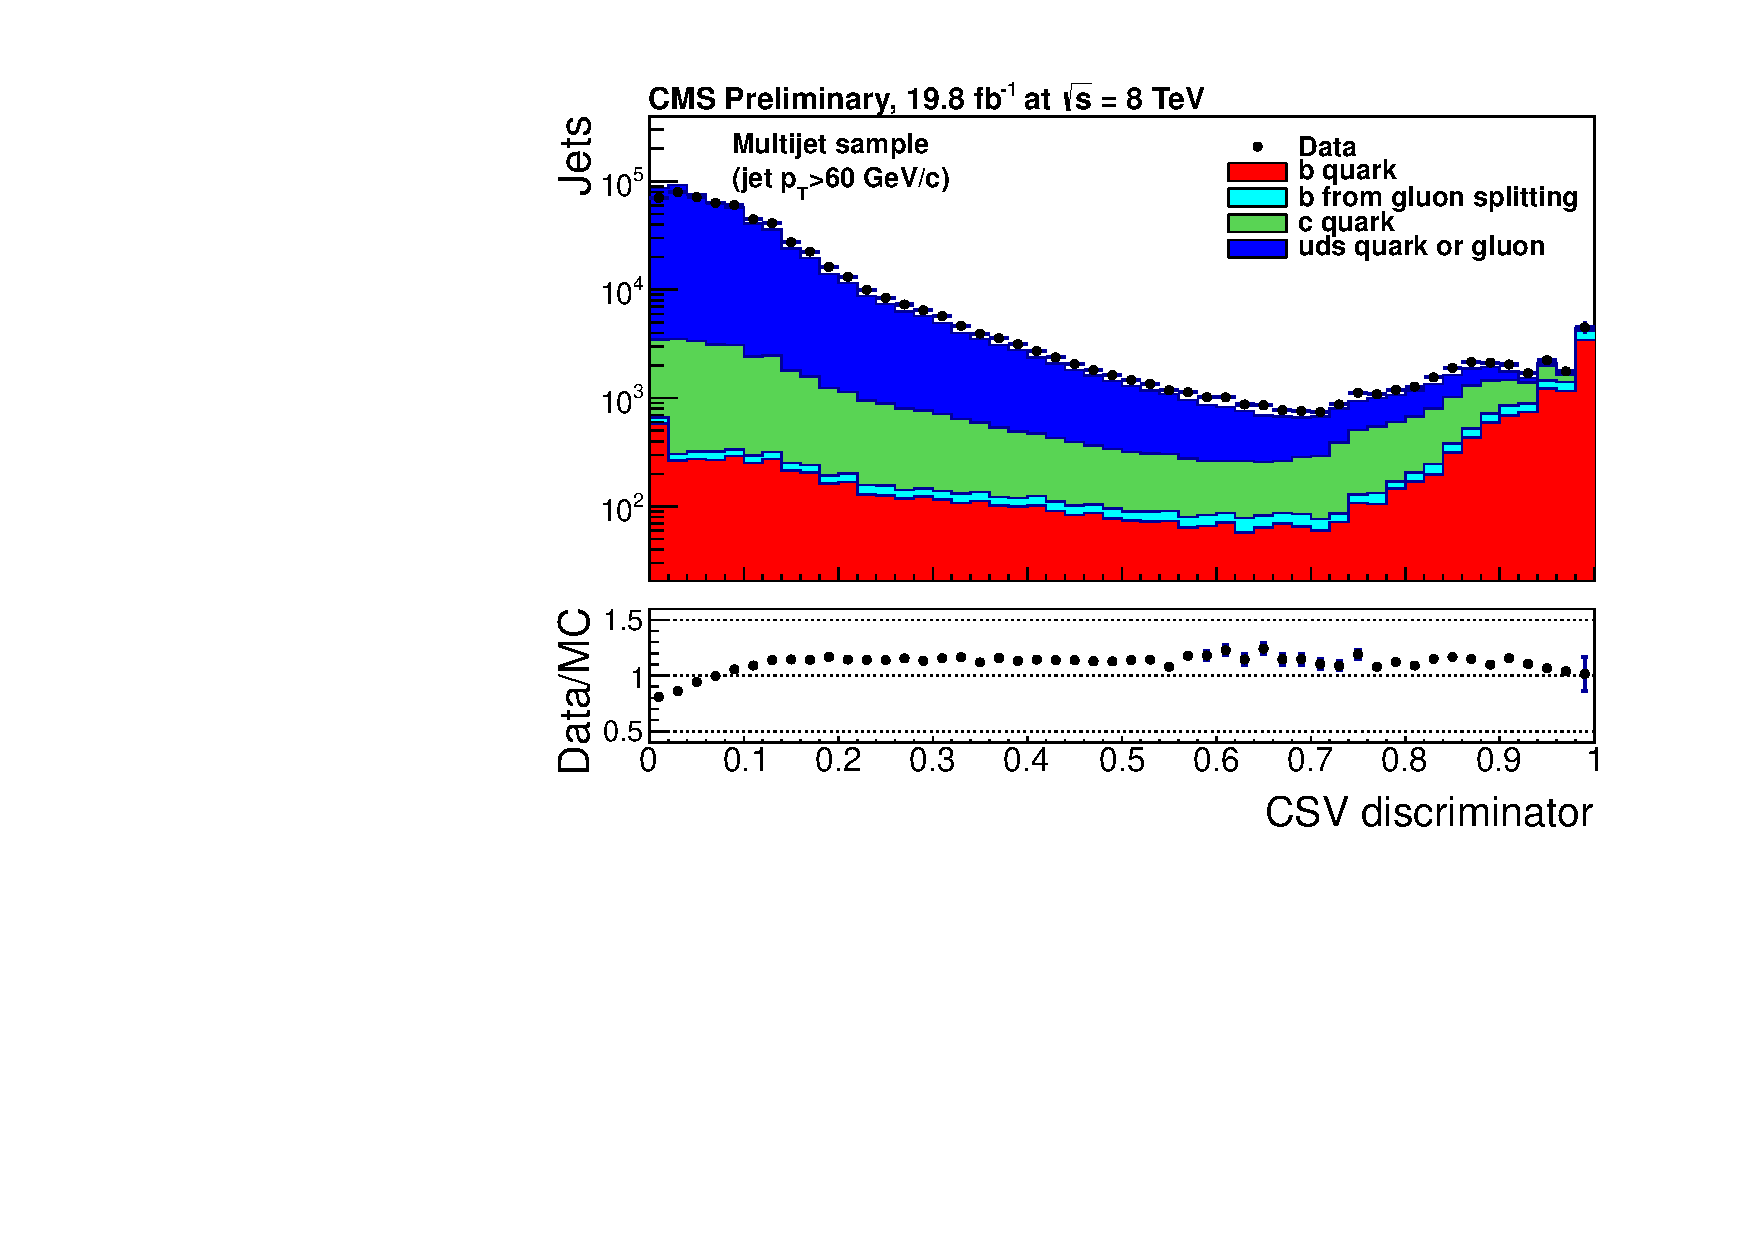
\includegraphics[width=0.45\textwidth]{\chsix/CSV-multijet-run1.pdf}}
\subfigure[]{\label{fig:csv_813TeV_b}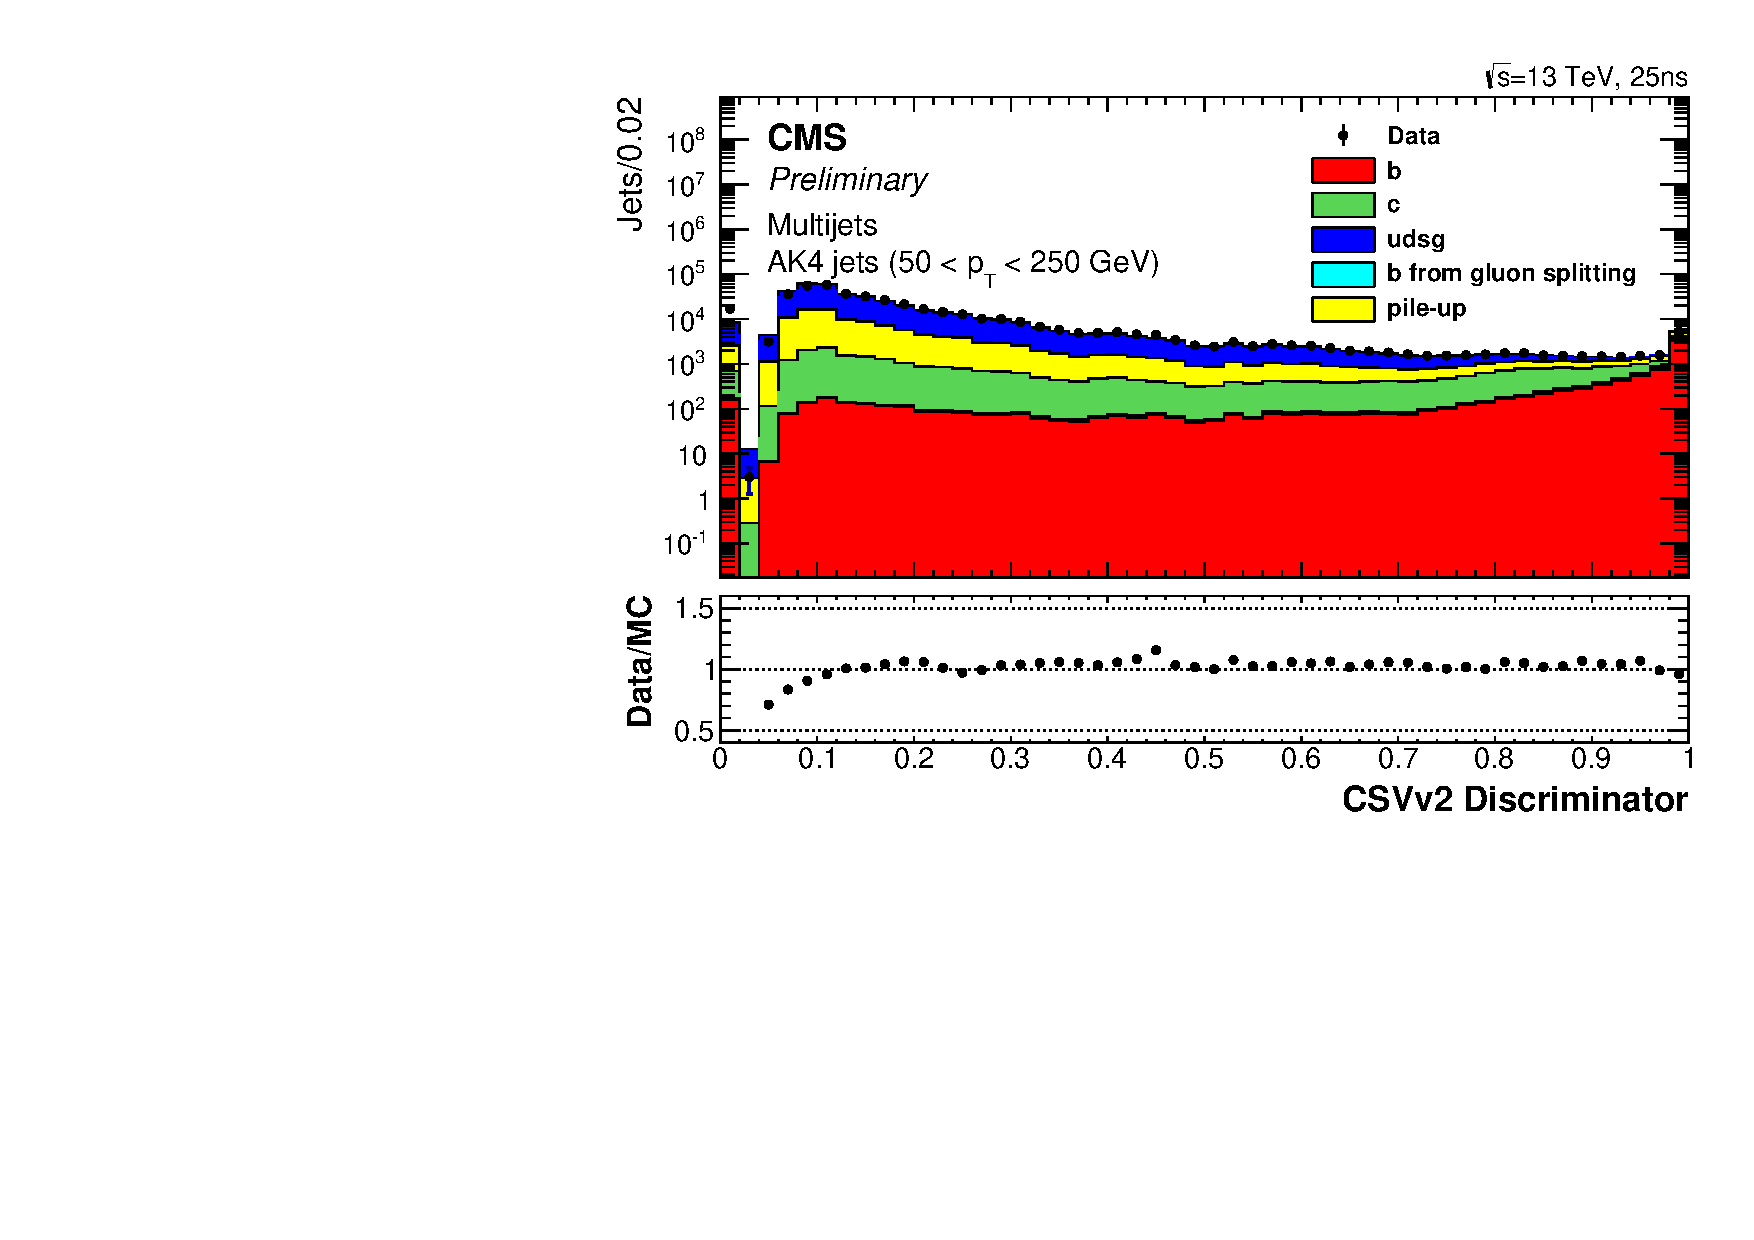
\includegraphics[width=0.45\textwidth]{\chsix/CSVv2-multijet-run2.pdf}}
\end{center} 
\caption{(a) Distribution of the CSV discriminator value in a multijet sample for data collected at 8\TeV and for simulation~\cite{CMS:BTV13001}, for jets reconstructed with the AK5 algorithm. (b) Distribution of the CSVv2 discriminator value in a multijet sample for data collected at 13\TeV and for simulation, for jets reconstructed with the AK4 algorithm~\cite{CMS-PAS-BTV-15-001}.}
\label{fig:csv_813TeV}
\end{figure}

The CSV algorithm was further optimized for Run~2 and the new version is referred to as CSV version 2 (CSVv2)~\cite{CMS-PAS-BTV-15-001}. The main differences with respect to the Run~1 version of the CSV algorithm are the different vertex reconstruction algorithm used, the number of input variables and the way those are combined. As in the previous version, the input variables are combined using a multivariate technique. However, the method previously used limited the amount of input variables since correlations between those could not be taken into account properly. In addition, the secondary vertex information is obtained with the IVF method described above. Figure~\ref{fig:csv_813TeV_b} shows the distribution of the CSVv2 discriminator value in a multijet sample for 13\TeV data and for simulation, for jets clustered with the AK4 algorithm.

The performance of the CSVv2 tagger is presented in Fig.~\ref{fig:btagalgo} as the b-jet identification efficiency versus the misidentification probability for jets in simulated \ttbar events requiring jet $\pt > 30\GeV$. A comparison is shown with the Run~1 version of the CSV algorithm trained for 8\TeV pp collisions using AK5 jets. The absolute improvement of the CSVv2 algorithm with respect to the CSV is of the order of 2 to 4\% in b-jet identification efficiency when comparing at the same misidentification probability for light-flavour jets. The improvement of using IVF vertices with respect to using AVR vertices in the CSVv2 algorithm is of the order of 1 to 2\%.\\
%For light-flavour jets, the absolute efficiency improves by about 4\% with respect to the CSVv2 algorithm.

\begin{figure}[!htb]
 \begin{center}
  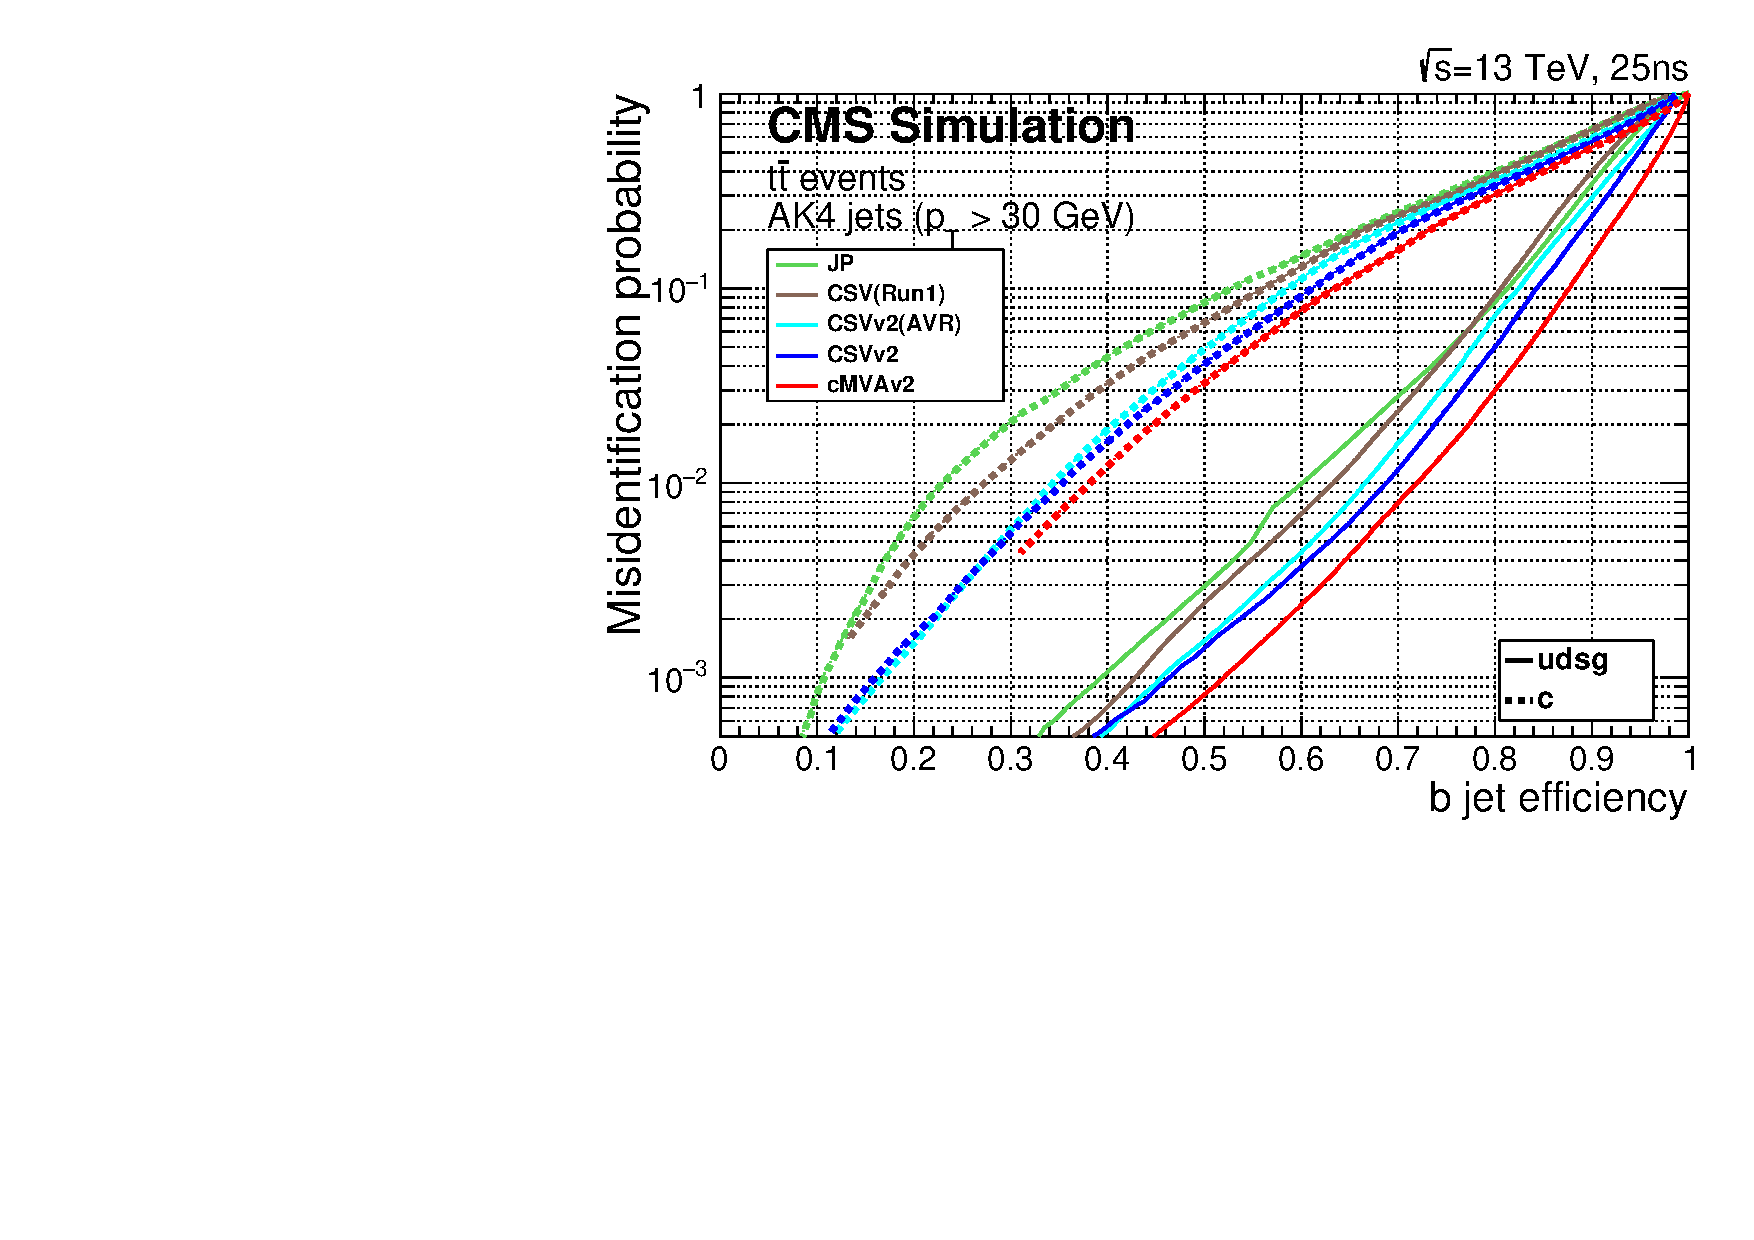
\includegraphics[width=0.45\textwidth]{\chsix/btagalgo-ak4jets.pdf}
 \end{center}
 \caption{Performance of the CSVv2 algorithm showed as the probability for non-b jets to be misidentified as b jet as a function of the efficiency to correctly identify as b jets. The improvement of this algorithm with respect to the Run~1 version is also shown~\cite{CMS-PAS-BTV-15-001}.}
 \label{fig:btagalgo}
\end{figure}

The value of the discriminator threshold for the b-tagging algorithms used in this analysis and the corresponding efficiencies are presented in Table~\ref{tab:btagwp}.
In this analysis the medium working point is used to identify and reject \ttbar events where a real b jet is expected in addition to the large-cone jet used to reconstruct the $\PV\to\qqbar$ or $\PH\to\bbbar$ candidate, representing instead the signal. The same b-tagging algorithm but together with the loose working point is used to identify whether the CA8 jet comes from a H boson decaying into bottom quarks, as described in Section~\ref{sec:htagging}.

\begin{table}[!htb]
\centering
\caption{B taggers and discriminator threshold used in CMS for Run~1 and Run~2 and corresponding efficiency for b jets with $\pt > 30\GeV$ in simulated \ttbar events. }
\resizebox{\textwidth}{!}{
\begin{tabular}{ l | c | c | c}
Algorithm & Operating point & Discriminator value & B-tagging efficiency (\%)\\ 
\hline
\hline
\multirow{3}{*}{CSV (Run 1)} & CSVL & 0.244 & 80\\
 & CSVM & 0.679 &  64\\
 & CSVT & 0.898 & 42\\
\multirow{3}{*}{CSVv2 (Run 2)} & CSVv2L & 0.460 & 83\\
 & CSVv2M & 0.800 & 69\\
 & CSVvsT & 0.935 & 49\\
\end{tabular}}
\label{tab:btagwp}
\end{table}

The mismodelling of the b-tagging variables in simulation is taken into account by reweighting simulation event-by-event with the ratio of the b-tagging efficiency in data and simulation, determined in a sample enriched with b jets and depending on the jet \pt and $\eta$. The correction factors as a function of the b-jet \pt  are shown in Fig.~\ref{fig:btag_sfb_a} and~\ref{fig:btag_sfb_b} for the CSVM and CSVv2M operating points respectively, as measured in 8 and 13\TeV data. In a similar way, correction factors are also derived and applied to correct the misidentification probability in simulation. These factors are shown in Fig.~\ref{fig:btag_sfl_a} and~\ref{fig:btag_sfl_b} as a function of the jet \pt for the CSVM and CSVv2M operating points.
%The average scale factors are reported in Table~\ref{tab:btagwp} for the two b tagging algorithms used in this analysis. The average values of the correction factors $SF_\mathrm{b}$ are 0.95 and 0.93 for the CSVM, and CSVv2M algorithms, respectively. While average values of 1.17 for are obtained for $SF_\mathrm{light}$ for the CSVM algorithm.

\begin{figure}[!htb]
\begin{center}
\subfigure[]{\label{fig:btag_sfb_a}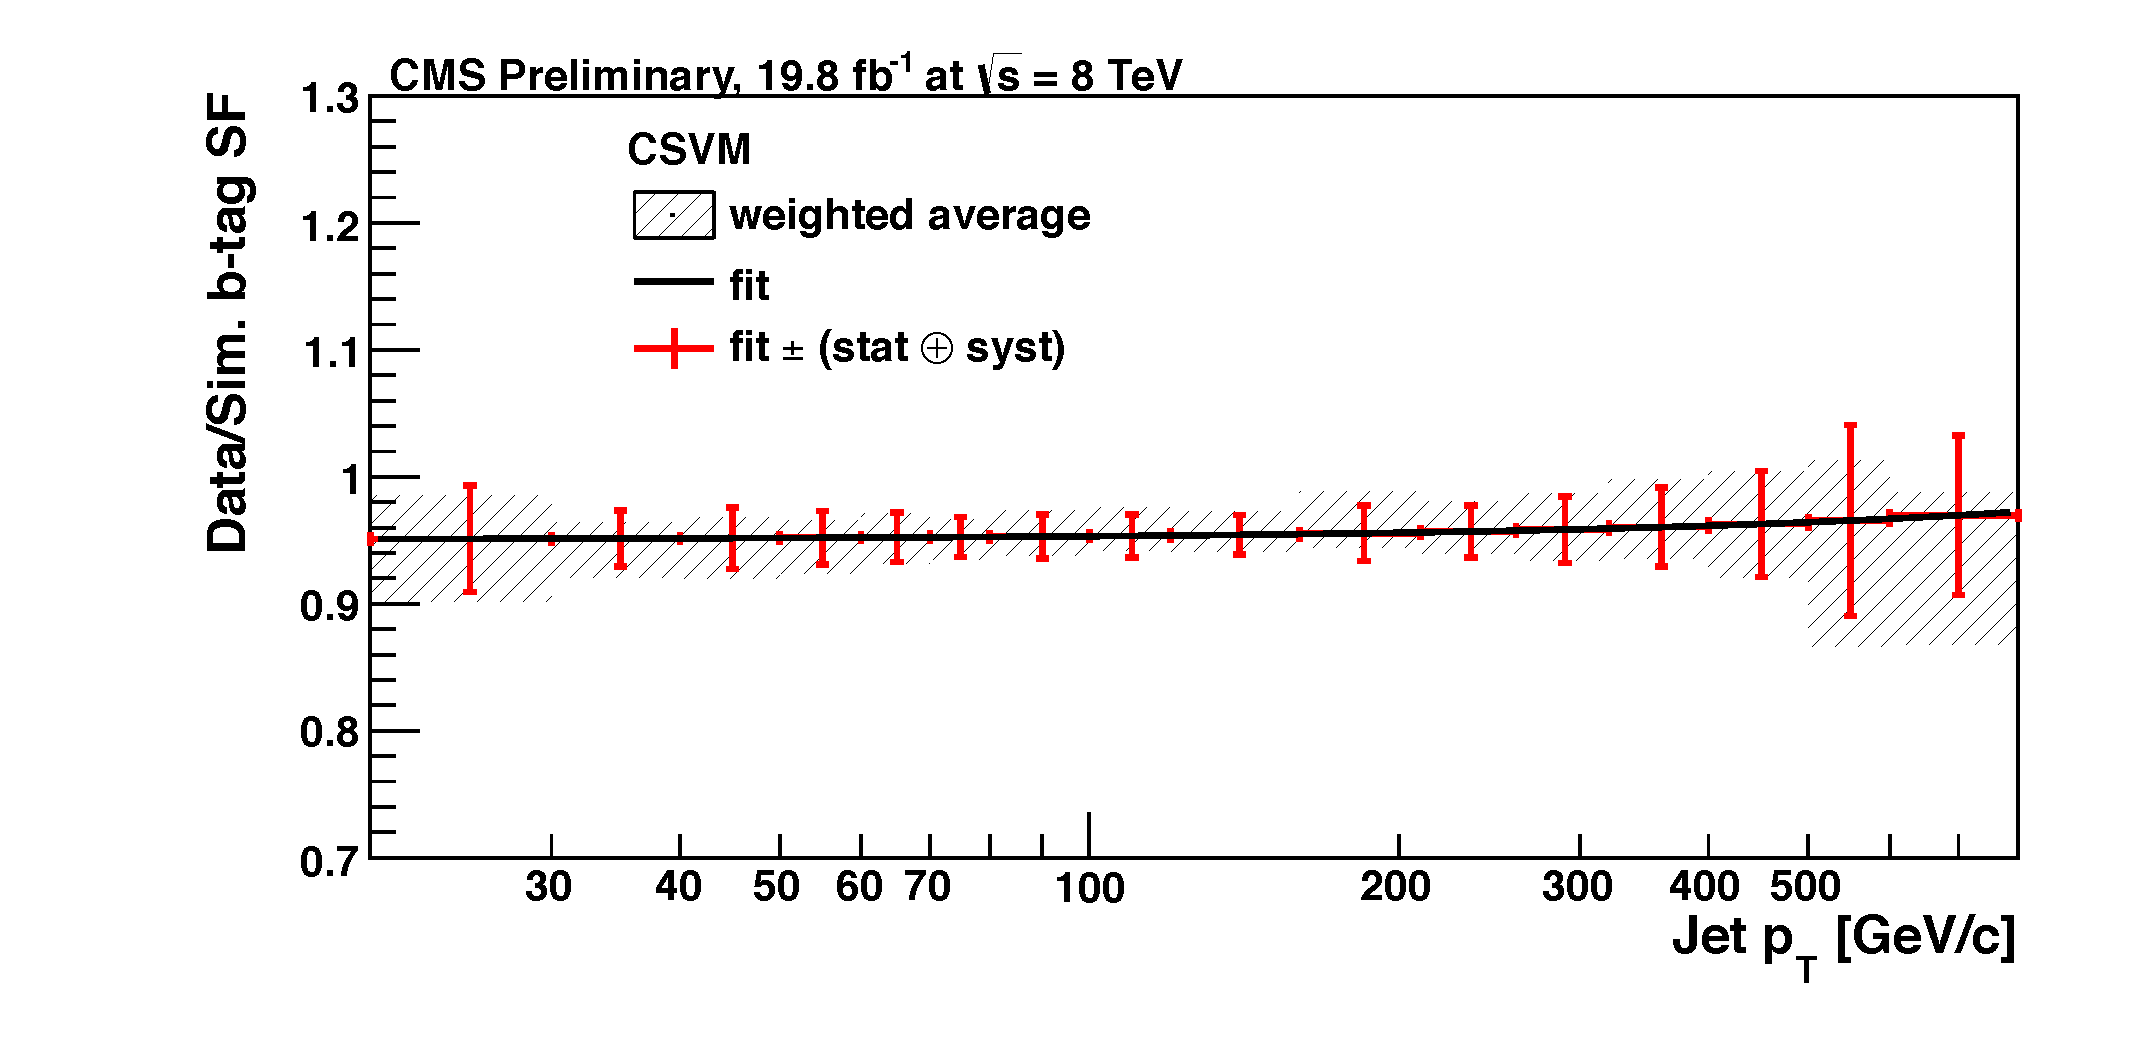
\includegraphics[width=0.45\textwidth]{\chsix/btag-sfb-pt-csvm-run1.pdf}}
\subfigure[]{\label{fig:btag_sfb_b}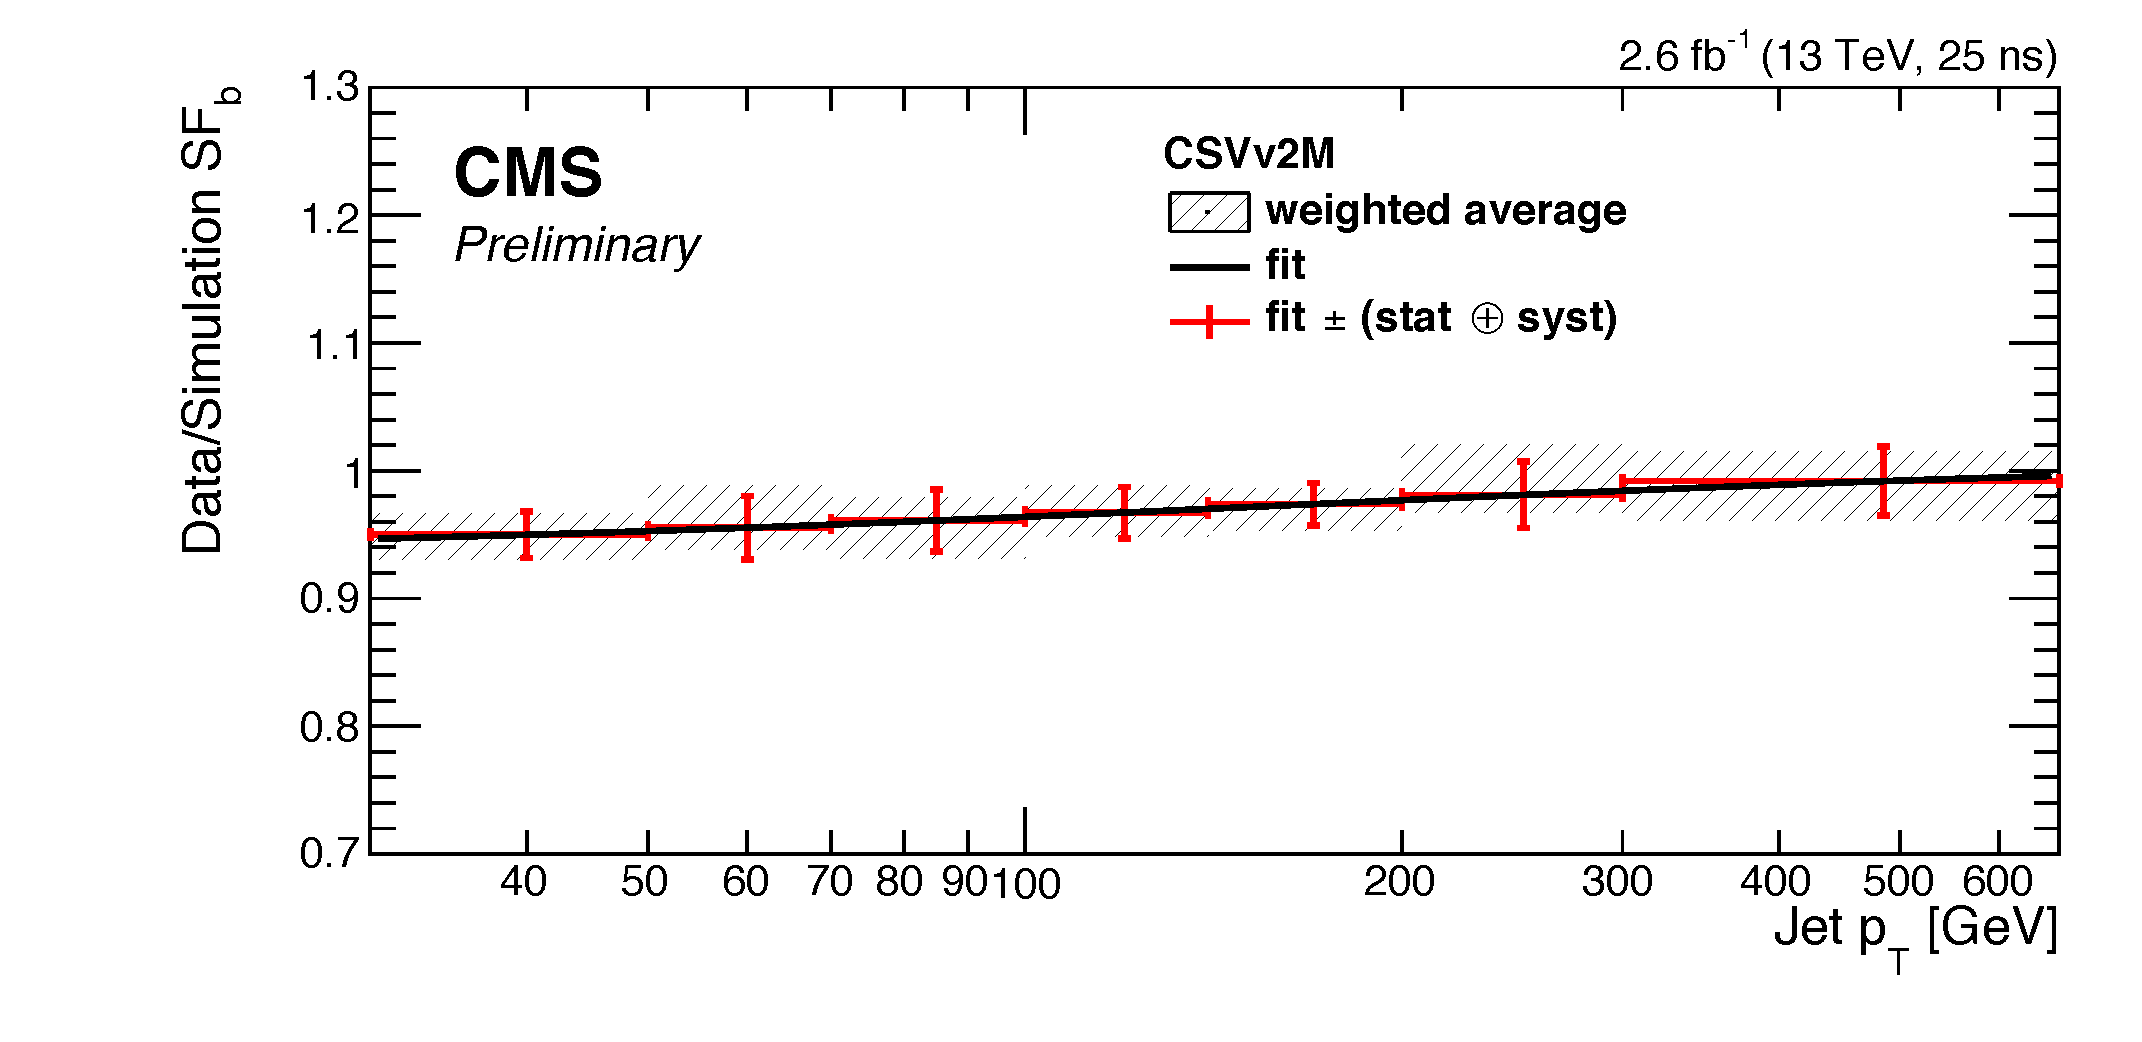
\includegraphics[width=0.45\textwidth]{\chsix/btag-sfb-pt-csvv2m-run2.pdf}}
\end{center} 
\caption{Data-to-simulation correction factors for the b-tagging efficiency for the CSVM (a) and CSVv2M (b) algorithms as a function of the b-jet \pt as measured in 8 and 13\TeV data~\cite{CMS:BTV13001,CMS-PAS-BTV-15-001}.}
\label{fig:btag_sfb}
\end{figure}

\begin{figure}[!htb]
\begin{center}
\subfigure[]{\label{fig:btag_sfl_a}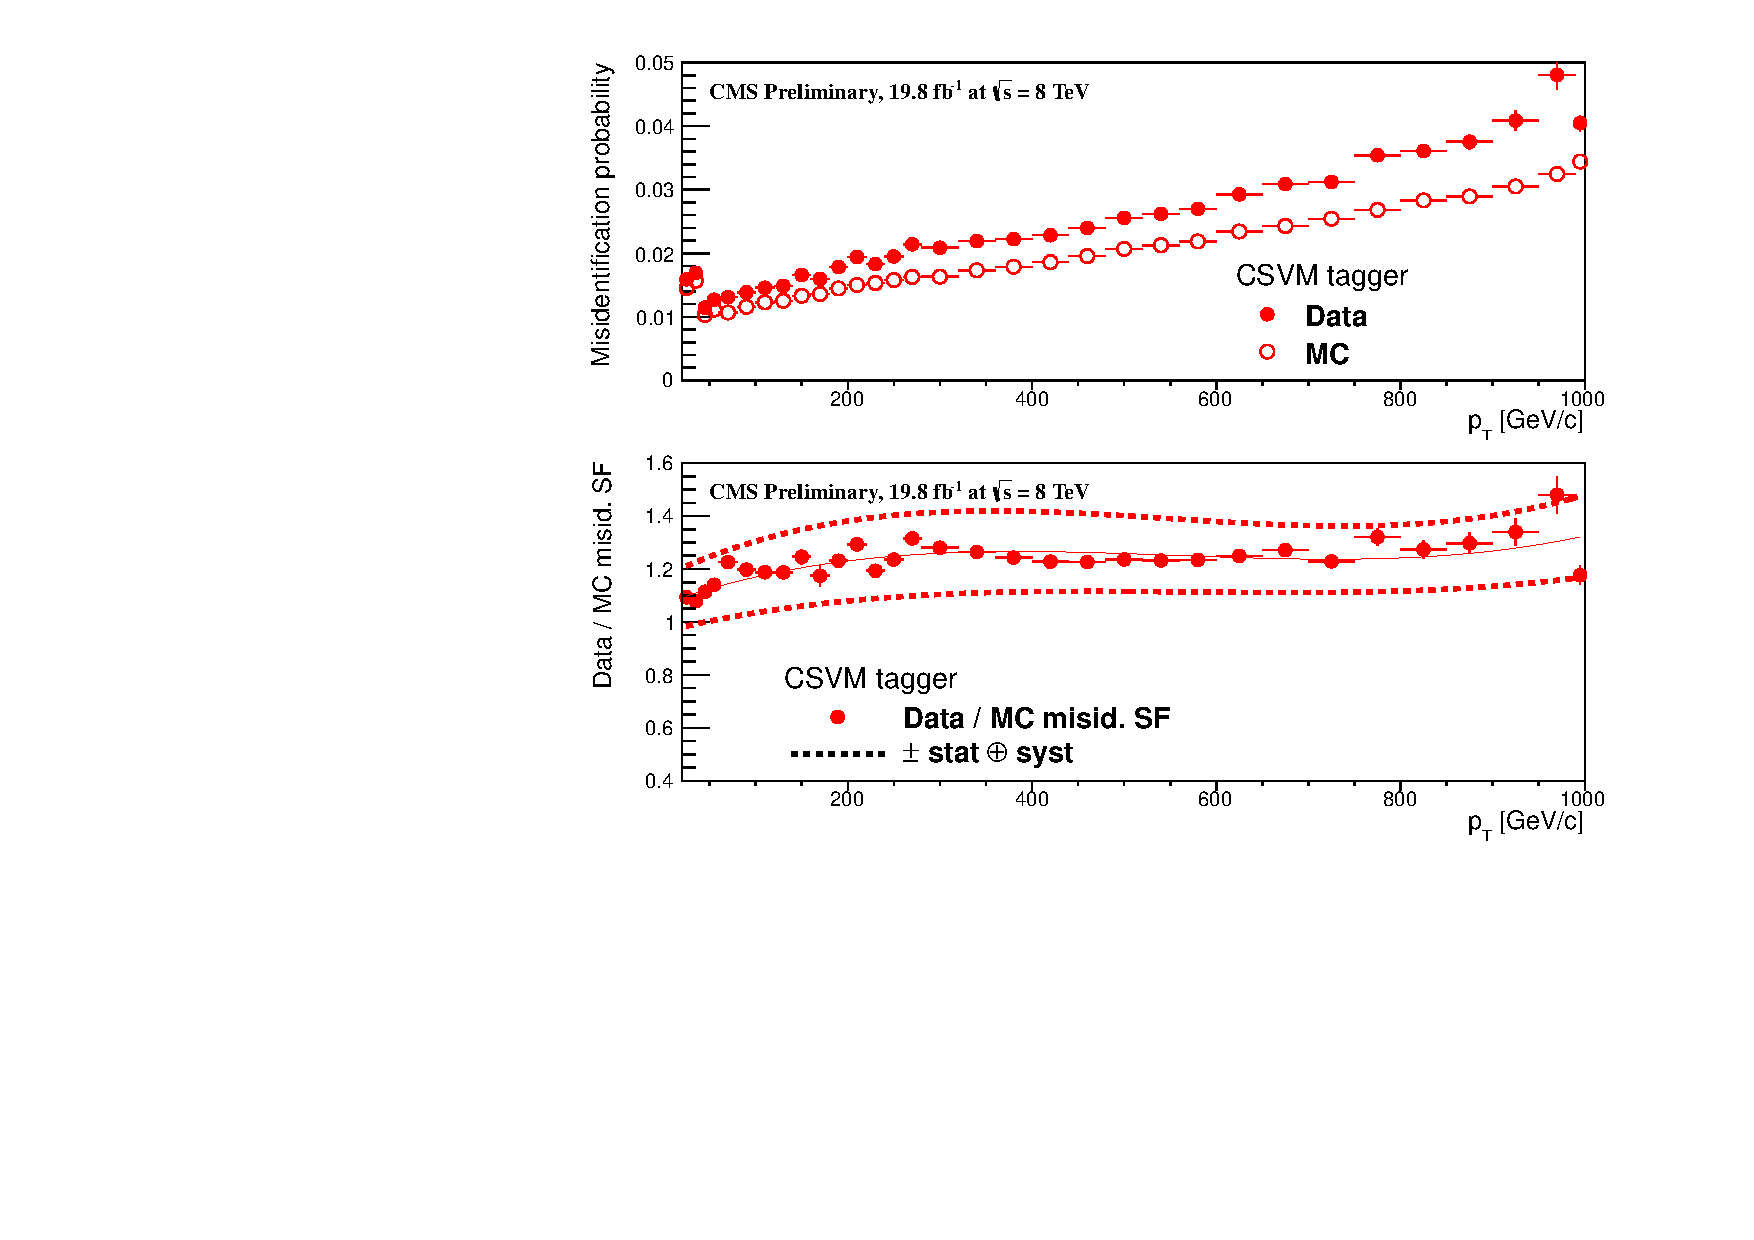
\includegraphics[width=0.45\textwidth]{\chsix/btag-SFlight-csvm-run1.pdf}}
\subfigure[]{\label{fig:btag_sfl_b}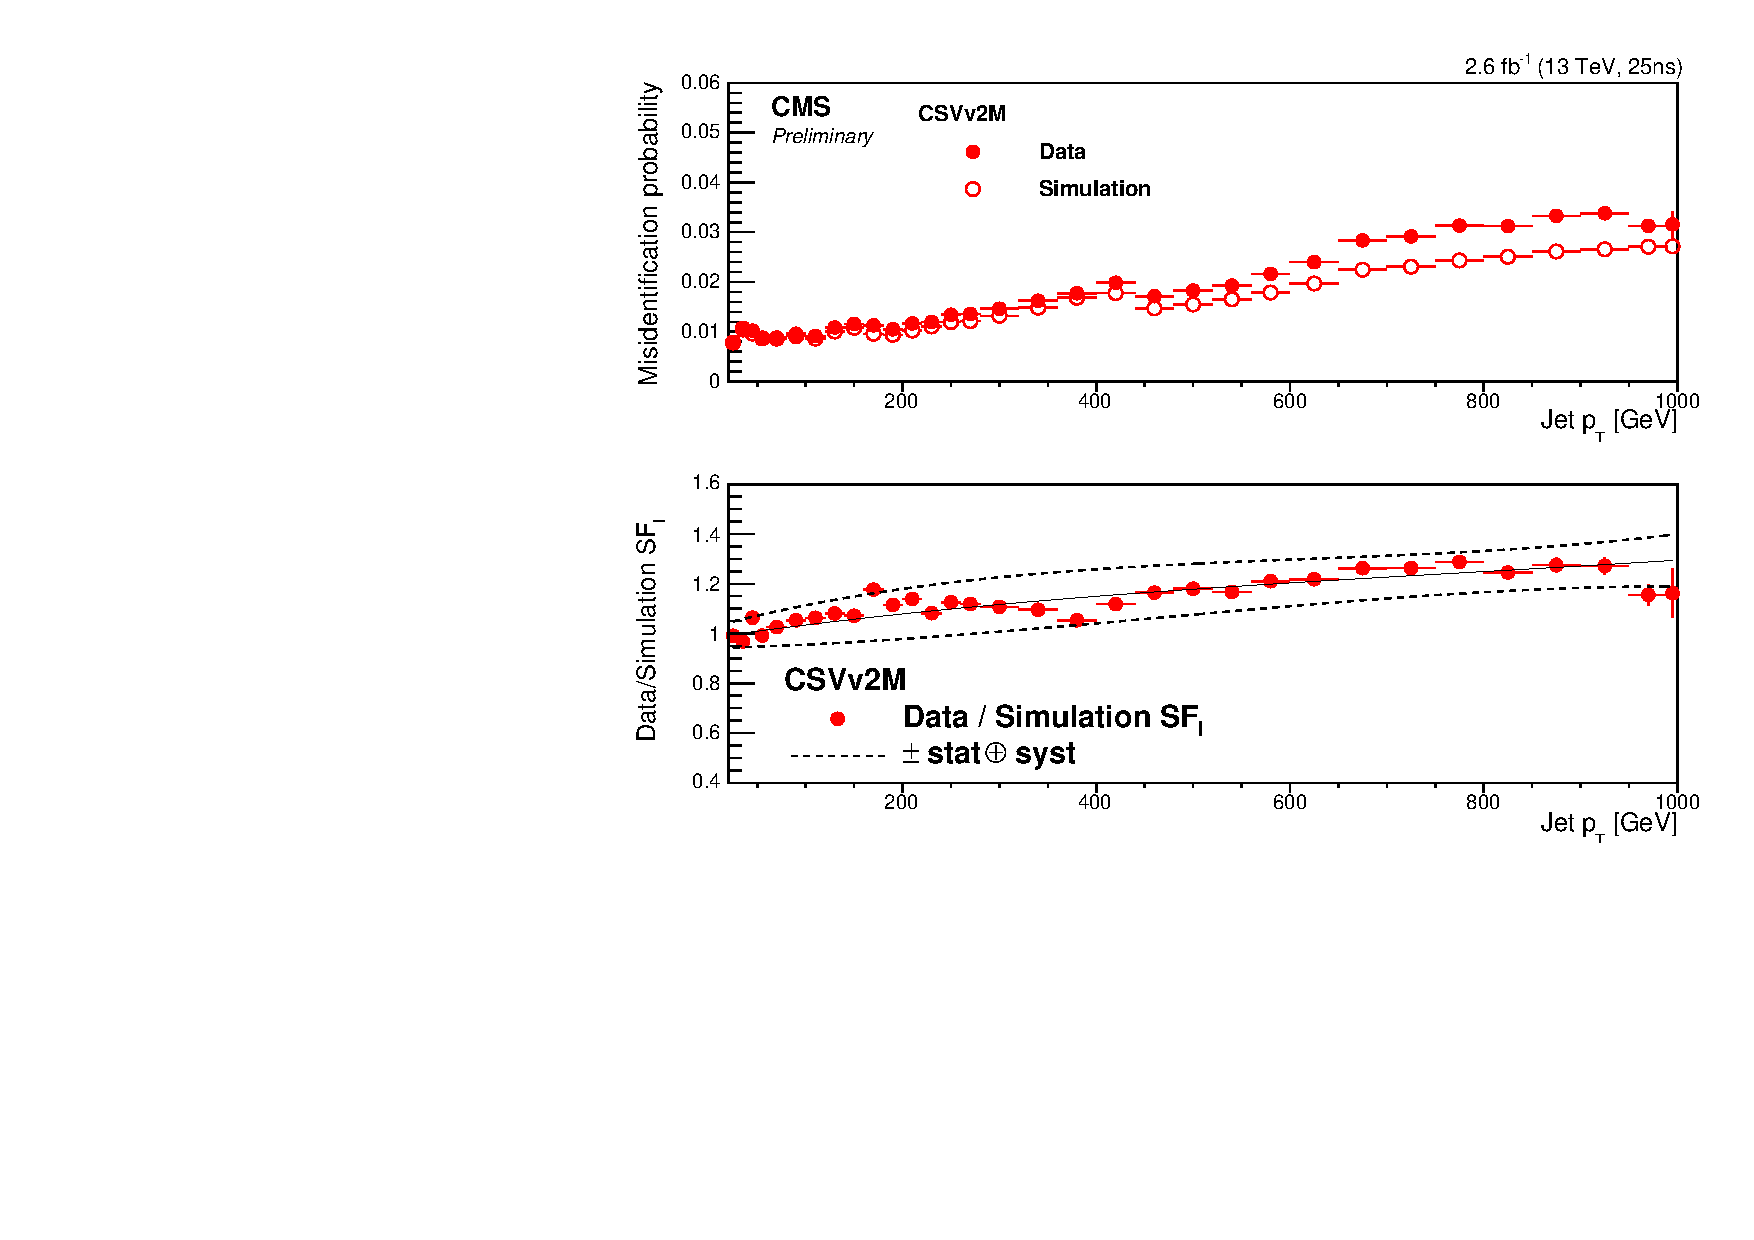
\includegraphics[width=0.45\textwidth]{\chsix/btag-SFlight-csvv2m-run2.pdf}}
\end{center} 
\caption{Data-to-simulation correction factors for the misidentification probability for the CSVM (a) and CSVv2M (b) algorithms as a function of the jet \pt as measured in 8 and 13\TeV data~\cite{CMS:BTV13001,CMS-PAS-BTV-15-001}.}
\label{fig:btag_sfl}
\end{figure}

%%%%%%%%%%
%\section{Missing transverse energy}\label{sec:met}
  %%%%%%%%%%%%%%%%%%%%%%%%%%%%%%%%%%%%%%%%%%%%%%%%%%%%%%%%%%%%%%%
\section{Missing transverse energy}\label{sec:met}
%%%%%%%%%%%%%%%%%%%%%%%%%%%%%%%%%%%%%%%%%%%%%%%%%%%%%%%%%%%%%%%

CMS is a full coverage hermetic detector which identifies and reconstructs almost all stable or long-lived particles produced in pp collisions. 
The only exceptions are neutrinos and hypothetical neutral weakly-interacting particles.
Although these particles do not leave a signal in the detector, their presence can be inferred from the momentum imbalance in the transverse plane,
a quantity known as missing transverse momentum and denoted by \ptvecmiss.

The standard method available in CMS for the reconstruction of \ptvecmiss uses the PF algorithm~\cite{1748-0221-6-09-P09001}.
%Several standard methods are available in CMS for the reconstruction of \ptvecmiss, which, as for the jet reconstruction, can be based on calorimeter information only, include also tracker information, or use the PF algorithm~\cite{1748-0221-6-09-P09001}. 
The PF \ptvecmiss is used in this analysis along with PF jets and it is calculated as the negative vector sum of the transverse momenta of all reconstructed PF candidates in a given event

\begin{equation}
\ptvecmiss = -\sum_{i}^{N}{\vec p}_{\mathrm{T},i}.
\end{equation}

Its magnitude is referred to as missing transverse energy and denoted by \ETmiss.
The \ETmiss is an important variable in many searches for physics beyond the standard model such as the ones described in this thesis where a real highly energetic neutrino is expected in the final state.
In addition, the precise measurement of \ETmiss plays a crucial role for measurements of standard model physics involving W and Z bosons and top quarks.
The \ptvecmiss reconstruction is sensitive to pileup, detector malfunctions and to various reconstruction effects. A precise calibration of all reconstructed physics objects is therefore crucial for its performance.
The level of mismeasurement is significantly reduced after jet energy calibration, described in Section~\ref{subsec:jetsreco}.
A correction to the \ptvecmiss is derived by propagating the jet energy scale corrections as described in the following.

The raw missing transverse momentum can be written as:

\begin{equation}
{\vec p}_\mathrm{T}^\mathrm{\; miss,raw} = - \sum_{i}^{N_\mathrm{jets}} {\vec p}_{\mathrm{T},i}^{\;\mathrm{raw}} - \sum_{i}^{N_\mathrm{uncl}} {\vec p}_{\mathrm{T},i},
\end{equation}

\noindent where the first and second sum runs over the \pt of the PF candidates clustered as jets and unclustered, respectively, and the superscript ``raw'' indicates the uncorrected value.
The correction to the \ptvecmiss is then obtained by replacing the first sum with the vector sum of the transverse momenta of the jets to which jet energy scale corrections (JEC) are applied:

\begin{equation}
{\vec C}_\mathrm{T}^\mathrm{JEC} = \sum_{i}^{N_\mathrm{jets}} {\vec p}_{\mathrm{T},i}^{\;\mathrm{raw}} - \sum_{i}^{N_\mathrm{jets}} {\vec p}_{\mathrm{T},i}^{\;\mathrm{JEC}},
\end{equation}

where the sum is performed over all jets with corrected $\pt > 10\GeV$.
This term is then added to the raw ${\vec p}_\mathrm{T}^\mathrm{\; miss,raw}$ to yield the corrected value:

\begin{equation}
{\vec p}_\mathrm{T}^\mathrm{\; miss,JEC} = {\vec p}_\mathrm{T}^\mathrm{\; miss,raw} + {\vec C}_\mathrm{T}^\mathrm{JEC} = - \sum_{i}^{N_\mathrm{jets}} {\vec p}_{\mathrm{T},i}^{\;\mathrm{JEC}} - \sum_{i}^{N_\mathrm{uncl}} {\vec p}_{\mathrm{T},i}.
\end{equation}

%Further corrections improve the performance of the \ptvecmiss reconstruction in events with large numbers of pileup interactions. This is achieved as explained in the following.
%
%The raw \ptvecmiss can be written as a sum of the two contributions due to particles produced in the primary vertex (PV) and in pileup interactions (PU)
%
%\begin{equation}\label{eqn:metraw}
%{\vec p}_\mathrm{T}^\mathrm{\; miss,raw} = - \sum_{i \in \mathrm{PV}} {\vec p}_{\mathrm{T},i} - \sum_{i \in \mathrm{PU}} {\vec p}_{\mathrm{T},i}.
%\end{equation}
%
%Particles produced in the pileup interactions can be further classified into neutral (PUneu) and charged (PUch) particles so that the equation above can be expressed as
%
%\begin{equation}
%{\vec p}_\mathrm{T}^\mathrm{\; miss,raw} = - \sum_{i \in \mathrm{PV}} {\vec p}_{\mathrm{T},i} - \sum_{i \in \mathrm{PUch}} {\vec p}_{\mathrm{T},i} - \sum_{i \in \mathrm{PUneu}} {\vec p}_{\mathrm{T},i}.
%\end{equation}
%
%The contribution to the genuine \ptvecmiss from such interactions is close to zero, as the probability to produce neutrinos is small in inelastic pp scattering interactions (e.g. neutrinos from Kaon decays).
%The vectorial \Vpt sum of charged particles is therefore expected to be well balanced by that of neutral particles.
%However, the nonlinearity and minimum energy thresholds in the calorimeters cause \ptvecmiss to point on average in the direction of the vectorial \Vpt sum of neutral particles.
%Nevertheless, it can be assumed that the directions of neutral pileup particles is measured with high precisions from the positions of the calorimeter cells in which we observe the energy deposits, while their energies are systematically off by the same factor. At the same time, the CMS tracker can also measure very well the charged pileup particles from their large curvature due to the low \pt characterizing this type of processes.
%With these assumptions, the total contribution from pileup can be estimated as
%
%\begin{equation}
%{\vec \Delta}_\mathrm{PU} = \sum_{i \in \mathrm{PUch}} {\vec p}_{\mathrm{T},i} + \sum_{i \in \mathrm{PUneu}} {\vec p}_{\mathrm{T},i} = \sum_{i \in PU} f({\vec v}) {\vec v},
%\end{equation}
%
%where ${\vec v}$ represents the sum of the transverse momenta of charged particles for each pileup interaction.
%The correction $f({\vec v})$ is parametrized as $f({\vec v}) = c_1 (1.0 +erf(-c_2|{\vec v}^{c_3}|))$, where the coefficients $c_1$, $c_2$, and $c_3$ are extracted from simulated minimum bias events.
%The corrected \ptvecmiss is then obtained by removing the additional contribution ${\vec \Delta}_\mathrm{PU}$ from Eq.~\ref{eqn:metraw}
%
%\begin{equation}
%{\vec p}_\mathrm{T}^\mathrm{\; miss,PUcorr} = {\vec E}_\mathrm{T}^\mathrm{\; miss,raw} + {\vec \Delta}_\mathrm{PU}.
%\end{equation}
%
Another type of correction is derived and applied to correct for a modulation in $\phi$ in the \ptvecmiss present not only in data but also in simulation. The distribution of genuine \ptvecmiss is instead independent of $\phi$ because of the rotational symmetry of the collisions around the beam axis. The possible causes of the modulation include imperfect detector alignment, inefficiencies, a residual \pt dependence of the calibration, and a shift between the center of the detector and the beam line. The correction for this effect can be expressed as a shift in the \ptvecmiss components along the $x$ and $y$ detector coordinates, which increases approximately linearly with the number of reconstructed vertices. This correlation is used for a correction procedure as follows

\begin{equation}
\begin{split}
{\vec E}_{\mathrm{T},x}^\mathrm{\; miss,\phi corr} & = {\vec E}_{\mathrm{T},x}^\mathrm{\; miss,raw} - (c_{x_0} + c_{x_s}N_\mathrm{vtx}),\\
{\vec E}_{\mathrm{T},y}^\mathrm{\; miss,\phi corr} & = {\vec E}_{\mathrm{T},y}^\mathrm{\; miss,raw} - (c_{y_0} + c_{y_s}N_\mathrm{vtx}),
\end{split}
\end{equation}

\noindent where the coefficients are determined separately for data and simulated events.
%Other more sophisticated missing energy determinations aimed at improving the resolution have been developed in CMS\cite{Khachatryan:2014gga,CMS-PAS-JME-16-004} but will not be discussed in this section since they are not used in this work.\\

The distributions of the PF \ETmiss, obtained after applying all the corrections described above, in $\PZ\to\MM$, $\PZ\to\EE$, and prompt photon events are presented in Fig.~\ref{fig:met_distr} as measured in 8\TeV data and for simulation. Good agreement between data and simulation is observed in all distributions.

These events contain no genuine \ptvecmiss, and thus a balance exists between the well-measured vector-boson transverse momentum, denoted as ${\vec q}_\mathrm{T}$, and the hadronic recoil, denoted as ${\vec u}_\mathrm{T}$,  which dominates the \ptvecmiss measurement. The $q_\mathrm{T}$ can therefore be used as a reference to measure the scale and resolution of \ptvecmiss.
The hadronic recoil can be projected along the axis defined by $q_\mathrm{T}$, yielding two signed components, parallel ($u_\parallel$) and perpendicular ($u_\perp$) to this axis. The parallel component is typically negative as the observed hadronic system is usually in the hemisphere opposite the boson. The scalar quantity $-\left\langle u_\parallel\right\rangle/{\vec q}_\mathrm{T}$ is referred to as the \ptvecmiss response. The response curves, extracted from the data as a function of the vector boson boost ${\vec q}_\mathrm{T}$, are shown in Fig.~\ref{fig:met_resol_a}, where deviations from unity indicate a bias on the hadronic recoil energy scale which is  fully recovered for ${\vec q}_\mathrm{T} > 40\GeV$.
%The bias is fully recovered for ${\vec q}_\mathrm{T} > 40\GeV$, while below this value the uncorrected unclustered energy contribution starts to be significant compared to the corrected energy of the recoiling jets, leading to an underestimation of the response.
%A reasonable agreement is found between data and simulation.
%The curves fit to $\gamma$ + jets data are 2?3\% lower than those fit to Z data at ${\vec q}_\mathrm{T} < 100\GeV$. This effect primarily stems from the large contribution of QCD multijet events to the ${\vec q}_\mathrm{T} < 100\GeV$ region of the selected photon sample. In these QCD multijet events, the hadronic recoil of the photon candidate tends to have a higher contamination of gluon jets. As the calorimeter response to gluon jets is characteristically lower than for quark jets due to difference of jet composition and collimation, the overall average response is reduced for the photon sample in this region.
The resolution curves, $\sigma(u_\parallel)$ and $\sigma(u_\perp)$ as a function of $q_\mathrm{T}$, are shown in Fig.~\ref{fig:met_resol_b} and~\ref{fig:met_resol_c}, respectively, for each control sample. The resolution increases with increasing $q_\mathrm{T}$, while the data and simulation curves are in good agreement for each control sample.\\

\begin{figure}[!htb]
\begin{center}
\subfigure[]{\label{fig:met_distr_a}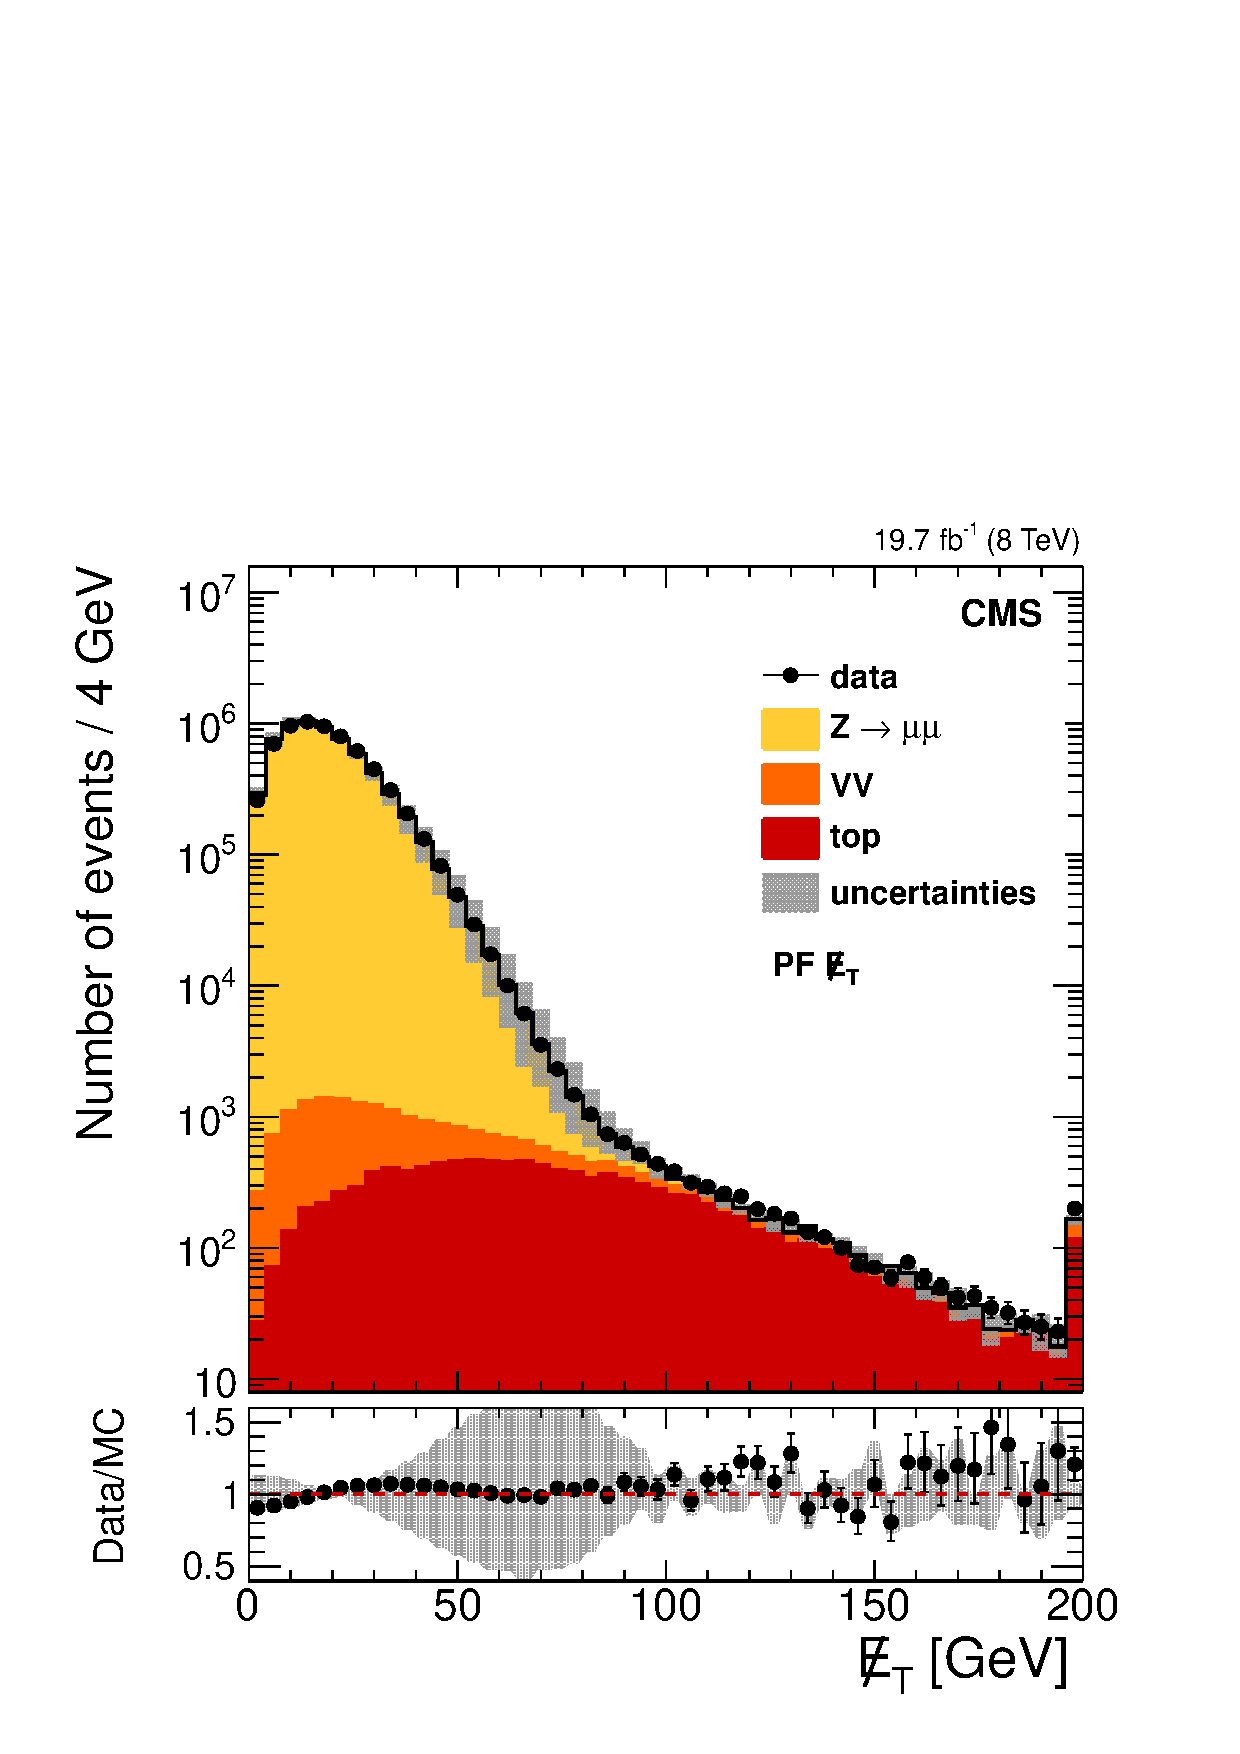
\includegraphics[width=0.3\textwidth]{\chsix/met-run1-type1phi-zmm.pdf}}
\subfigure[]{\label{fig:met_distr_b}\includegraphics[width=0.3\textwidth]{\chsix/met-run1-type1phi-zee.pdf}}
\subfigure[]{\label{fig:met_distr_c}\includegraphics[width=0.3\textwidth]{\chsix/met-run1-type1phi-zgg.pdf}}
\end{center} 
\caption{The PF \ETmiss distribution in $\PZ\to\MM$ (a), $\PZ\to\EE$ (b), and prompt photon (c) events for 8\TeV data and for simulation. The points in the lower panel of each plot show the ratio between data and simulation describing their agreement~\cite{Khachatryan:2014gga}.}
\label{fig:met_distr}
\end{figure}

\begin{figure}[!htb]
\begin{center}
\subfigure[]{\label{fig:met_resol_a}\includegraphics[width=0.3\textwidth]{\chsix/met-run1-type1phi-resp.pdf}}
\subfigure[]{\label{fig:met_resol_b}\includegraphics[width=0.3\textwidth]{\chsix/met-run1-type1phi-resopara.pdf}}
\subfigure[]{\label{fig:met_resol_c}\includegraphics[width=0.3\textwidth]{\chsix/met-run1-type1phi-resoperp.pdf}}
\end{center} 
\caption{(a) Response curves for PF \ptvecmiss in events with a Z boson or prompt photon.
Also shown are the resolution curves of the parallel (b) and perpendicular (b) recoil components as a function of the Z/$\gamma$ $q_\mathrm{T}$. 
In each plot the upper frame shows the response in 8\TeV data, while the lower one shows the ratio between data and simulation.~\cite{Khachatryan:2014gga}.}
\label{fig:met_resol}
\end{figure}

 
%%%%%%%%%%
%\section{W$\rightarrow\ell\Pgn$ reconstruction}\label{sec:leptonicW}
   %%%%%%%%%%%%%%%%%%%%%%%%%%%%%%%%%%%%%%%%%%%%%%%%%%%%%%%%%%%%%%%
\section{W$\rightarrow\ell\Pgn$ reconstruction}\label{sec:leptonicW}
%%%%%%%%%%%%%%%%%%%%%%%%%%%%%%%%%%%%%%%%%%%%%%%%%%%%%%%%%%%%%%%

The identified muon or electron (see Section~\ref{subsec:eleid} and~\ref{subsec:muonid}) is associated with the W$\rightarrow\ell\nu$ candidate. 
The \pt of the undetected neutrino is assumed to be equal to the \ETmiss. The longitudinal momentum of the neutrino ($p_z$) is obtained by solving a quadratic equation that sets the $\ell\nu$ invariant
mass to the known W boson mass~\cite{Agashe:2014kda}:

\begin{equation}\label{eqn:pzv}
M_\mathrm{W}^2 = m_\ell^2   + 2(E_\ell E_\nu - p_{x_\ell}p_{x_\nu} - p_{y_\ell}p_{y_\nu} - p_{z_\ell}p_{z_\nu} ) = (80.4)^2
\end{equation}

In the case of two real solutions, the one with the smaller absolute value is chosen; in the case of two complex solutions, only the real part is used.
The four-momentum of the neutrino is used to reconstruct the four-momentum of the W$\rightarrow\ell\nu$ candidate.
The same procedure is applied for W$\rightarrow\tau\nu$ candidates, where the $\tau$ decays to one muon or electron and two neutrinos.
In this case, the \Etmiss represents the \pt of the three-neutrino system.


In the case of two real solutions, the one with the smaller absolute value is chosen. 
If the discriminant becomes negative, or equivalently $M_\mathrm{T}$ is larger than $M_\mathrm{W}$ used in the constraint, the solutions have an imaginary part. This happens because of the finite resolution of \ETmiss.
Several schemes exist to deal with this situation. One technically simple method consists of taking the real part of the complex solutions but it leads to the wrong W boson mass. This method is used for the reconstruction of the W$\rightarrow\ell\nu$ candidate in the 13\TeV analysis described in this work.

A second method is also studied here, which eliminates the imaginary component by modifying the components of the missing transverse energy such to give $M_\mathrm{T} =  M_\mathrm{W}$, still respecting equation~\ref{eqn:pzv}~\cite{BauerPhd10}. This method is used in the 8\TeV analysis described in this work for the reconstruction of the W$\rightarrow\ell\nu$ candidate and for the reconstruction of the mass of the leptonically decaying top quark in \ttbar events. The performance of the two methods are equivalent in terms of resolution of the reconstructed diboson invariant mass.

%%%%%%%%%%
\section{Summary}

A detailed description of the reconstruction of the objects present in the lepton+jet final states under study has been provided in this chapter, and a summary is given in the following.\\

Section~\ref{sec:tracksandvtx} was focused on the reconstruction of the tracks and primary vertices in the event.
The trajectories of charged particles are reconstructed through an iterative procedure that uses the reconstructed hits in the silicon detectors to determine the track parameters, i.e. the \pt, the azimuthal and polar angles, and the transverse and longitudinal impact parameters.
The primary vertices are reconstructed from a set of well-reconstructed tracks.
All events are required to have at least one primary vertex reconstructed within a 24\cm window along the beam axis, with a transverse distance from the nominal pp interaction region of less than 2\cm. In the presence of more than one vertex passing these requirements, the primary-interaction vertex, where the hard process of interest takes place, is chosen to be the one with the highest total $\pt^2$, summed over all the associated tracks.\\

The following two sections, namely Sections~\ref{sec:electrons} and~\ref{sec:muons}, were devoted to the reconstruction and identification of electrons and muons, respectively.

Electron candidates are reconstructed by matching energy deposits in the ECAL with reconstructed tracks. In order to suppress multijet background, electron candidates must pass stringent quality criteria tuned for high-\pt objects and an isolation selection. The total scalar sum of the \pt of all the tracks in a cone of radius $\Delta R = 0.3$ around the electron direction, excluding tracks within an inner cone of $\Delta R = 0.04$ to remove the contribution from the electron itself, divided by the electron \pt, is required be less than 5\%. In addition, a calorimetric isolation parameter is calculated by summing the energies of reconstructed deposits in both ECAL and HCAL, not associated with the electron itself, within a cone of radius $\Delta R = 0.3$ around the electron. The upper threshold for this isolation parameter depends on the electron kinematic quantities and the average amount of additional energy coming from pileup interactions.

Muons are reconstructed through a fit to the hits in both the inner tracking system and the muon spectrometer.
They must satisfy identification requirements on the impact parameters of the track, the number of hits reconstructed in both the silicon tracker and the muon detectors, and the uncertainty in the \pt measurement.
These quality criteria ensure a precise measurement of the four-momentum and reject misreconstructed muons.
An isolation requirement is applied to suppress background from multijet events where jet constituents are identified as muons.
Specifically, the scalar sum of the \pt of all other tracks in a cone of radius $\Delta R = 0.3$ around but not including the muon track must be less than 10\% of the muon \pt.

The triggers used in this analysis have also been described in Sections~\ref{sec:electrons} and~\ref{sec:muons}. They require either one muon or one electron, without isolation requirements and with loose identification criteria.
A minimum value for the \pt of the lepton is required, which is higher for the data collected in pp collisions at 13\TeV.
Specifically, the electrons selected by the trigger must have $\et > 80$ and 105\GeV for the 8 and 13\TeV data analysis, respectively,
whereas the thresholds on the \pt of the muons are 40 and 45\GeV. In addition, the electrons and muons must have $\eta < 2.5$ and 2.1, respectively.
The efficiency for an electron passing the identification and isolation requirements summarized above to fire the single-electron trigger has been measured to be 98--99\%.
The efficiency for the single-muon trigger varies between 80 and 95\%, and between 92 and 98\%, for the 8 and 13\TeV analysis, respectively, depending on the $\eta$ of the muon.\\

The jet reconstruction in CMS has been described in Section~\ref{sec:jets}.
Jets are clustered from the four-momenta of the particles reconstructed by the PF algorithm, which reconstructs individual particles by combining information from all sub-detector systems.
The reconstructed PF constituents are assigned to one of the five candidate categories (electrons, muons, photons, charged hadrons, and neutral hadrons) and used as input to the chosen jet-clustering algorithm.
In order to mitigate biases in the reconstruction due to PU interactions, in the jet-clustering procedure charged PF particles not associated with the primary-interaction vertex are excluded.

The CA and AK jet-clustering algorithms with a distance parameter $R = 0.8$ are used to identify the $\PH\to\bbbar$ and $\PV\to\qqbar$ candidates in the 8 and 13\TeV data analysis, respectively.
In order to identify b jets, the AK jet-clustering algorithm is used with a distance parameter $R = 0.5$ and 0.4 for the 8 and 13\TeV data analysis, respectively.
In addition, the CSV b-tagging algorithm is applied to the reconstructed AK4 and AK5 jets using a working point that provides a misidentification rate of 1\% and efficiency of 64--69\%.
The ratio of the b-tagging efficiency between data and simulation is used as a scale factor to correct the simulated events.
A correction based on the projected area of the jet on the front face of the calorimeter is used to take into account the extra energy clustered in jets due to neutral particles coming from pileup.
Jet energy corrections are derived from simulation and from dijet and photon+jet events in data.
Additional quality criteria are applied to the jets in order to remove spurious jet-like features originating from isolated noise patterns
in the calorimeters or the tracker. The efficiency of these jet quality requirements for real jets is above 99\%.

For the 8\TeV data analysis, the CA8 (AK5) jets are required to be separated from any well-identified electron or muon by $\Delta R > 0.8$ (0.3).
In addition, all AK5 and CA8 jets must have $\pt > 30\GeV$ and $> 200\GeV$, respectively, and $|\eta| < 2.4$ to be considered in the subsequent steps of the analysis.
The AK5 jets are required to be separated from the CA8 jet representing the $\PV\to\qqbar$ candidate by $\Delta R > 0.8$.
Finally, CA8 jets are not used in the analysis if their pseudorapidity falls in the region $1.0 < |\eta| < 1.8$, thus overlapping the barrel-endcap transition region of the silicon tracker where the reconstruction is not optimal for the objects relevant to this analysis. The same selections are applied for AK4 and AK8 jets in the 13\TeV data analysis, except for the aforementioned fiducial cut on the $\eta$ of the large-cone jet since the reconstruction issue was fixed for Run~2.\\

As described in Section~\ref{sec:met}, the missing transverse energy is estimated through the magnitude of the vector sum of the transverse momenta of the reconstructed PF objects.
The value of the \ETmiss so obtained is modified to account for corrections to the energy scale of all the reconstructed AK5 or AK4 jets in the event.
In addition, a correction applied to correct for a modulation in $\phi$ in the \ptvecmiss due to imperfect detector alignment, inefficiencies, a residual \pt dependence of the calibration, and a shift between the center of the detector and the beam line.\\

Finally, the $\PW\to\ell\nu$ candidate is formed from the combination of electron and muon candidates with the \ptvecmiss,
where an estimate of the neutrino longitudinal momentum is derived through the methods described in Section~\ref{sec:leptonicW},
which imposes the constraint of the W-boson mass on the invariant mass of the $\ell\Pgn$ system.